%Page Setup, don't remove
\documentclass[12pt]{book} 
\setlength{\columnsep}{0.7truecm}
\setlength{\parindent}{0cm}
\usepackage[top=2truecm,bottom=2.8truecm, left=2.2truecm, right=2.2truecm,headsep=10pt, paperwidth=19.3truecm, paperheight=27.6truecm]{geometry} 
\usepackage[usenames,dvipsnames,table]{xcolor}
\usepackage{tcolorbox}
\definecolor{ocre}{RGB}{52,177,201} 
\usepackage{pdfpages}
\usepackage{avant}
\usepackage{bussproofs}
\usepackage{mathptmx}
%\usepackage{ebgaramond}
 \usepackage{xeCJK}
 \setCJKmainfont{SimSun}
\usepackage{tikz}
\usepackage{tkz-euclide}
\usepackage{matchsticks}
\usepackage{wrapfig}
\usepackage{listings}
\usepackage[utf8]{vietnam}
\usepackage{babel}
\usepackage[LSBC5,T1]{fontenc}

%----------------------------------------------------------------------------------------
%	VARIOUS REQUIRED PACKAGES
%----------------------------------------------------------------------------------------
\usepackage{titlesec} % Allows customization of titles
\usepackage{multicol}
\usepackage{graphicx} % Required for including pictures
%\graphicspath{{Pictures/}} % Specifies the directory where pictures are stored
\usepackage{lipsum} % Inserts dummy text
\usepackage{tikz} % Required for drawing custom shapes
%\usepackage{enumitem} % Customize lists
%\setlist{nolistsep} % Reduce spacing between bullet points and numbered lists
\usepackage{booktabs} % Required for nicer horizontal rules in tables
\usepackage{eso-pic} % Required for specifying an image background in the title page
\usepackage{titletoc} % Required for manipulating the table of contents
\contentsmargin{0cm} % Removes the default margin
\usepackage{adjustbox} 
\usepackage{amsmath,amsfonts,amssymb,amsthm} % For math equations, theorems, symbols, etc
%\usepackage[framemethod=tikz]{mdframed} 
\usepackage[sexy]{evan}
\usepackage{hyperref}
\urlstyle{same}
\usepackage{tikz} % figure in two column
\usepackage{float}
\usepackage{biblatex}
\usepackage{caption}% dinh dang figure caption
%\usepackage[font=normalsize]{caption}
\usepackage{changepage}
\usepackage{booktabs}

\usepackage{chngcntr}
\usepackage{array}
\usepackage{eurosym}
\usepackage{multirow}
\usepackage{mathtools}
\usepackage{setspace}
\usepackage{afterpage}
\usepackage{scalerel}
\usepackage{blindtext}
\usepackage{tabularx}
\usepackage{afterpage}
\usepackage{array}
%\usepackage{transparent}
\usepackage{efbox}
\usepackage{tabulary}
% \usepackage{CJKutf8}
\usepackage{subcaption}
\usepackage{rotating}
\usepackage{microtype}
\usepackage{pgfplots}

\usetikzlibrary{lindenmayersystems}
\usetikzlibrary{shapes,shapes.geometric}
\usetikzlibrary{decorations.pathreplacing}
\usetikzlibrary{calc,intersections}
\usetikzlibrary[shadings]
\usetikzlibrary{decorations.fractals}

\newmdenv[skipabove=7pt,
skipbelow=7pt,
backgroundcolor=black!5,
linecolor=ocre,
leftline=true,
innerleftmargin=6pt,
innerrightmargin=6pt,
innertopmargin=8pt,
leftmargin=0cm,
rightmargin=0cm,
innerbottommargin=8pt]{tBox}

\def\PIbox#1{\tikz\node[draw = ocre,fill=black!5,align=justify,text width=.95\linewidth,inner sep=2mm]{#1};}%
\renewcommand{\qedsymbol}{}	
\usepackage{fancyhdr} % Required for header and footer configuration
%%%% Header for duong vao toan hoc
\fancypagestyle{duongvaotoanhoc}{
	\fancyhf{}
	\fancyhead[E]{
		\insertpic{63}{740}{1}{duongvao1}
		\insertpic{333}{35}{1}{fduongvao1}
}
	\fancyhead[O]{
		\insertpic{1}{740}{1}{duongvao2}
		\insertpic{59}{34.9}{1}{fduongvao2}
}	
\renewcommand{\footrulewidth}{0pt}
\fancyfoot[LE,RO]{\sffamily\footnotesize	\thepage}

\fancyfoot[LO,RE]{\sffamily\scriptsize TẬP 7 -- SỐ 11 THÁNG 11/2023}
}

\fancypagestyle{duongvaotoanhocnone}{
	\fancyhf{}
	\fancyhead[E]{
		\insertpic{333}{35}{1}{fduongvao1}
	}
	\fancyhead[O]{
		\insertpic{59}{34.9}{1}{fduongvao2}
	}	
	\renewcommand{\footrulewidth}{0pt}
	\fancyfoot[LE,RO]{\sffamily\footnotesize	\thepage}
	
	\fancyfoot[LO,RE]{\sffamily\scriptsize TẬP 7 -- SỐ 11 THÁNG 11/2023}
}

\fancypagestyle{thachthuctoanhoc}{
	\fancyhf{}
	\fancyhead[E]{
		\insertpic{63}{740}{1}{thachthuc1}
		\insertpic{333}{35}{1}{fthachthuc1}
	}
	\fancyhead[O]{
		\insertpic{1}{740}{1}{thachthuc2}
		\insertpic{59}{34.9}{1}{fthachthuc2}
	}	
	\renewcommand{\footrulewidth}{0pt}
	\fancyfoot[LE,RO]{\sffamily\footnotesize	\thepage}
	
	\fancyfoot[LO,RE]{\sffamily\scriptsize TẬP 7 -- SỐ 11 THÁNG 11/2023}
}

\fancypagestyle{thachthuctoanhocnone}{
	\fancyhf{}
	\fancyhead[E]{
		\insertpic{333}{35}{1}{fthachthuc1}
	}
	\fancyhead[O]{
		\insertpic{59}{34.9}{1}{fthachthuc2}
	}	
	\renewcommand{\footrulewidth}{0pt}
	\fancyfoot[LE,RO]{\sffamily\footnotesize	\thepage}
	
	\fancyfoot[LO,RE]{\sffamily\scriptsize TẬP 7 -- SỐ 11 THÁNG 11/2023}
}


%%%% Header for Toán học và đời sống
\fancypagestyle{toanhocvadoisong}{
			\fancyhf{}
		\fancyhead[E]{
			\insertpic{63}{740}{1}{toanhocds1}
			\insertpic{333}{35}{1}{ftoanhocds1}
		}
		\fancyhead[O]{
			\insertpic{1}{740}{1}{toanhocds2}
			\insertpic{59}{34.9}{1}{ftoanhocds2}
		}	
		\renewcommand{\footrulewidth}{0pt}
		\fancyfoot[LE,RO]{\sffamily\footnotesize	\thepage}
		
		\fancyfoot[LO,RE]{\sffamily\scriptsize TẬP 7 -- SỐ 11 THÁNG 11/2023}
}
\fancypagestyle{toanhocvadoisongnone}{
	\fancyhf{}
	\fancyhead[E]{
		\insertpic{333}{35}{1}{ftoanhocds1}
	}
	\fancyhead[O]{
		\insertpic{59}{34.9}{1}{ftoanhocds2}
	}	
	\renewcommand{\footrulewidth}{0pt}
	\fancyfoot[LE,RO]{\sffamily\footnotesize	\thepage}
	
	\fancyfoot[LO,RE]{\sffamily\scriptsize TẬP 7 -- SỐ 11 THÁNG 11/2023}
}

\fancypagestyle{doisongtoanhoc}{
	\fancyhf{}
	\fancyhead[E]{
		\insertpic{63}{740}{1}{dstoanhoc1}
		\insertpic{333}{35}{1}{fdstoanhoc1}
	}
	\fancyhead[O]{
		\insertpic{1}{740}{1}{dstoanhoc2}
		\insertpic{59}{34.9}{1}{fdstoanhoc2}
	}	
	\renewcommand{\footrulewidth}{0pt}
	\fancyfoot[LE,RO]{\sffamily\footnotesize	\thepage}
	
	\fancyfoot[LO,RE]{\sffamily\scriptsize TẬP 7 -- SỐ 11 THÁNG 11/2023}
}
\fancypagestyle{doisongtoanhocnone}{
	\fancyhf{}
	\fancyhead[E]{
		\insertpic{333}{35}{1}{fdstoanhoc1}
	}
	\fancyhead[O]{
		\insertpic{59}{34.9}{1}{fdstoanhoc2}
	}	
	\renewcommand{\footrulewidth}{0pt}
	\fancyfoot[LE,RO]{\sffamily\footnotesize	\thepage}
	
	\fancyfoot[LO,RE]{\sffamily\scriptsize TẬP 7 -- SỐ 11 THÁNG 11/2023}
}

%%% doi thoai toan hoc
\fancypagestyle{doithoaitoanhoc}{
	\fancyhf{}
	\fancyhead[E]{
		\insertpic{63}{740}{1}{doithoai1}
		\insertpic{333}{35}{1}{fdoithoai1}
	}
	\fancyhead[O]{
		\insertpic{1}{740}{1}{doithoai2}
		\insertpic{59}{34.9}{1}{fdoithoai2}
	}	
	\renewcommand{\footrulewidth}{0pt}
	\fancyfoot[LE,RO]{\sffamily\footnotesize	\thepage}
	
	\fancyfoot[LO,RE]{\sffamily\scriptsize TẬP 7 -- SỐ 11 THÁNG 11/2023}
}
\fancypagestyle{doithoaitoanhocnone}{
	\fancyhf{}
	\fancyhead[E]{
		\insertpic{333}{35}{1}{fdoithoai1}
	}
	\fancyhead[O]{
		\insertpic{59}{34.9}{1}{fdoithoai2}
	}	
	\renewcommand{\footrulewidth}{0pt}
	\fancyfoot[LE,RO]{\sffamily\footnotesize	\thepage}
	
	\fancyfoot[LO,RE]{\sffamily\scriptsize TẬP 7 -- SỐ 11 THÁNG 11/2023}
}

%%%% Header for co dien hien dai
\fancypagestyle{codienhiendai}{
	\fancyhf{}
	\fancyhead[E]{
		\insertpic{63}{740}{1}{codien1}
		\insertpic{333}{35}{1}{fcodien1}
	}
	\fancyhead[O]{
		\insertpic{1}{740}{1}{codien2}
		\insertpic{59}{34.9}{1}{fcodien2}
	}	
	\renewcommand{\footrulewidth}{0pt}
	\fancyfoot[LE,RO]{\sffamily\footnotesize	\thepage}
	
	\fancyfoot[LO,RE]{\sffamily\scriptsize TẬP 7 -- SỐ 11 THÁNG 11/2023}
}
\fancypagestyle{codienhiendainone}{
	\fancyhf{}
	\fancyhead[E]{
		\insertpic{333}{35}{1}{fcodien1}
	}
	\fancyhead[O]{
		\insertpic{59}{34.9}{1}{fcodien2}
	}	
	\renewcommand{\footrulewidth}{0pt}
	\fancyfoot[LE,RO]{\sffamily\footnotesize	\thepage}
	
	\fancyfoot[LO,RE]{\sffamily\scriptsize TẬP 7 -- SỐ 11 THÁNG 11/2023}
}

\fancypagestyle{diendandayvahoctoan}{
	\fancyhf{}
	\fancyhead[E]{
		\insertpic{63}{740}{1}{diendan1}
		\insertpic{333}{35}{1}{fdiendan1}
	}
	\fancyhead[O]{
		\insertpic{1}{740}{1}{diendan2}
		\insertpic{59}{34.9}{1}{fdiendan2}
	}	
	\renewcommand{\footrulewidth}{0pt}
	\fancyfoot[LE,RO]{\sffamily\footnotesize	\thepage}
	
	\fancyfoot[LO,RE]{\sffamily\scriptsize TẬP 7 -- SỐ 11 THÁNG 11/2023}
}
\fancypagestyle{diendandayvahoctoannone}{
	\fancyhf{}
	\fancyhead[E]{
		\insertpic{333}{35}{1}{fdiendan1}
	}
	\fancyhead[O]{
		\insertpic{59}{34.9}{1}{fdiendan2}
	}	
	\renewcommand{\footrulewidth}{0pt}
	\fancyfoot[LE,RO]{\sffamily\footnotesize	\thepage}
	
	\fancyfoot[LO,RE]{\sffamily\scriptsize TẬP 7 -- SỐ 11 THÁNG 11/2023}
}

\fancypagestyle{cackithitoan}{
	\fancyhf{}
	\fancyhead[E]{
		\insertpic{63}{740}{1}{cackithi1}
		\insertpic{333}{35}{1}{fcackithi1}
	}
	\fancyhead[O]{
		\insertpic{1}{740}{1}{cackithi2}
		\insertpic{59}{34.9}{1}{fcackithi2}
	}	
	\renewcommand{\footrulewidth}{0pt}
	\fancyfoot[LE,RO]{\sffamily\footnotesize	\thepage}
	
	\fancyfoot[LO,RE]{\sffamily\scriptsize TẬP 7 -- SỐ 11 THÁNG 11/2023}
}
\fancypagestyle{cackithitoannone}{
	\fancyhf{}
	\fancyhead[E]{
		\insertpic{333}{35}{1}{fcackithi1}
	}
	\fancyhead[O]{
		\insertpic{59}{34.9}{1}{fcackithi2}
	}	
	\renewcommand{\footrulewidth}{0pt}
	\fancyfoot[LE,RO]{\sffamily\footnotesize	\thepage}
	
	\fancyfoot[LO,RE]{\sffamily\scriptsize TẬP 7 -- SỐ 11 THÁNG 11/2023}
}

\fancypagestyle{lichsutoanhoc}{
	\fancyhf{}
	\fancyhead[E]{
		\insertpic{63}{740}{1}{lichsu1}
		\insertpic{333}{35}{1}{flichsu1}
	}
	\fancyhead[O]{
		\insertpic{1}{740}{1}{lichsu2}
		\insertpic{59}{34.9}{1}{flichsu2}
	}	
	\renewcommand{\footrulewidth}{0pt}
	\fancyfoot[LE,RO]{\sffamily\footnotesize	\thepage}
	
	\fancyfoot[LO,RE]{\sffamily\scriptsize TẬP 7 -- SỐ 11 THÁNG 11/2023}
}
\fancypagestyle{lichsutoanhocnone}{
	\fancyhf{}
	\fancyhead[E]{
		\insertpic{333}{35}{1}{flichsu1}
	}
	\fancyhead[O]{
		\insertpic{59}{34.9}{1}{flichsu2}
	}	
	\renewcommand{\footrulewidth}{0pt}
	\fancyfoot[LE,RO]{\sffamily\footnotesize	\thepage}
	
	\fancyfoot[LO,RE]{\sffamily\scriptsize TẬP 7 -- SỐ 11 THÁNG 11/2023}
}

%%%% Header for Tìm hiểu khoa học
\fancypagestyle{timhieukhoahoc}{
		\fancyhf{}
	\fancyhead[E]{
		\insertpic{63}{740}{1}{timhieu1}
		\insertpic{333}{35}{1}{ftimhieu1}
	}
	\fancyhead[O]{
		\insertpic{1}{740}{1}{timhieu2}
		\insertpic{59}{34.9}{1}{ftimhieu2}
	}	
	\renewcommand{\footrulewidth}{0pt}
	\fancyfoot[LE,RO]{\sffamily\footnotesize	\thepage}
	
	\fancyfoot[LO,RE]{\sffamily\scriptsize TẬP 7 -- SỐ 11 THÁNG 11/2023}	
}
\fancypagestyle{timhieukhoahocnone}{
	\fancyhf{}
	\fancyhead[E]{
		\insertpic{333}{35}{1}{ftimhieu1}
	}
	\fancyhead[O]{
		\insertpic{59}{34.9}{1}{ftimhieu2}
	}	
	\renewcommand{\footrulewidth}{0pt}
	\fancyfoot[LE,RO]{\sffamily\footnotesize	\thepage}
	
	\fancyfoot[LO,RE]{\sffamily\scriptsize TẬP 7 -- SỐ 11 THÁNG 11/2023}	
}

%%%% Header for quan toan
\fancypagestyle{quantoan}{
		\fancyhf{}
		\fancyhead[E]{
		\insertpic{63}{740}{1}{quantoan1}
		\insertpic{333}{35}{1}{fquantoan1}
	}
	\fancyhead[O]{
		\insertpic{1}{740}{1}{quantoan2}
		\insertpic{59}{34.9}{1}{fquantoan2}
	}	
	\renewcommand{\footrulewidth}{0pt}
	\fancyfoot[LE,RO]{\sffamily\footnotesize	\thepage}
	
	\fancyfoot[LO,RE]{\sffamily\scriptsize TẬP 7 -- SỐ 11 THÁNG 11/2023}
}
\fancypagestyle{quantoannone}{
	\fancyhf{}
	\fancyhead[E]{
		\insertpic{333}{35}{1}{fquantoan1}
	}
	\fancyhead[O]{
		\insertpic{59}{34.9}{1}{fquantoan2}
	}	
	\renewcommand{\footrulewidth}{0pt}
	\fancyfoot[LE,RO]{\sffamily\footnotesize	\thepage}
	
	\fancyfoot[LO,RE]{\sffamily\scriptsize TẬP 7 -- SỐ 11 THÁNG 11/2023}
}


\fancypagestyle{hoccungpi}{
				\fancyhf{}
		\fancyhead[E]{
			\insertpic{63}{740}{1}{hoccungpi1}
			\insertpic{333}{35}{1}{fhoccungpi1}
		}
		\fancyhead[O]{
			\insertpic{1}{740}{1}{hoccungpi2}
			\insertpic{59}{34.9}{1}{fhoccungpi2}
		}	
		\renewcommand{\footrulewidth}{0pt}
		\fancyfoot[LE,RO]{\sffamily\footnotesize	\thepage}
		
		\fancyfoot[LO,RE]{\sffamily\scriptsize TẬP 7 -- SỐ 11 THÁNG 11/2023}	
}
\fancypagestyle{hoccungpinone}{
	\fancyhf{}
	\fancyhead[E]{
		\insertpic{333}{35}{1}{fhoccungpi1}
	}
	\fancyhead[O]{
		\insertpic{59}{34.9}{1}{fhoccungpi2}
	}	
	\renewcommand{\footrulewidth}{0pt}
	\fancyfoot[LE,RO]{\sffamily\footnotesize	\thepage}
	
	\fancyfoot[LO,RE]{\sffamily\scriptsize TẬP 7 -- SỐ 11 THÁNG 11/2023}	
}

\fancypagestyle{toancuabi}{
	\fancyhf{}
	\fancyhead[E]{
		\insertpic{63}{740}{1}{toancuabi1}
		\insertpic{333}{35}{1}{ftoancuabi1}
	}
	\fancyhead[O]{
		\insertpic{1}{740}{1}{toancuabi2}
		\insertpic{59}{34.9}{1}{ftoancuabi2}
	}	
	\renewcommand{\footrulewidth}{0pt}
	\fancyfoot[LE,RO]{\sffamily\footnotesize	\thepage}
	
	\fancyfoot[LO,RE]{\sffamily\scriptsize TẬP 7 -- SỐ 11 THÁNG 11/2023}	
}
\fancypagestyle{toancuabinone}{
	\fancyhf{}
	\fancyhead[E]{
		\insertpic{333}{35}{1}{ftoancuabi1}
	}
	\fancyhead[O]{
		\insertpic{59}{34.9}{1}{ftoancuabi2}
	}	
	\renewcommand{\footrulewidth}{0pt}
	\fancyfoot[LE,RO]{\sffamily\footnotesize	\thepage}
	
	\fancyfoot[LO,RE]{\sffamily\scriptsize TẬP 7 -- SỐ 11 THÁNG 11/2023}	
}

\fancypagestyle{gocco}{
	\fancyhf{}
	\fancyhead[E]{
		\insertpic{63}{740}{1}{gocco1}
		\insertpic{333}{35}{1}{fgocco1}
	}
	\fancyhead[O]{
		\insertpic{1}{740}{1}{gocco2}
		\insertpic{59}{34.9}{1}{fgocco2}
	}	
	\renewcommand{\footrulewidth}{0pt}
	\fancyfoot[LE,RO]{\sffamily\footnotesize	\thepage}
	
	\fancyfoot[LO,RE]{\sffamily\scriptsize TẬP 7 -- SỐ 11 THÁNG 11/2023}	
}

\fancypagestyle{gocconone}{
	\fancyhf{}
	\fancyhead[E]{
		\insertpic{333}{35}{1}{fgocco1}
	}
	\fancyhead[O]{
		\insertpic{59}{34.9}{1}{fgocco2}
	}	
	\renewcommand{\footrulewidth}{0pt}
	\fancyfoot[LE,RO]{\sffamily\footnotesize	\thepage}
	
	\fancyfoot[LO,RE]{\sffamily\scriptsize TẬP 7 -- SỐ 11 THÁNG 11/2023}	
}
	
%	\fancyfoot[C]{\sffamily\footnotesize Tạp chí Pi } % Print the nearest section name on the left side of odd pages	


\pagestyle{fancy}
\renewcommand{\chaptermark}[1]{\markboth{\normalsize\bfseries\chaptername\ \thechapter.\ #1}{}} % Chapter text font settings
\renewcommand{\sectionmark}[1]{\markright{\normalsize\thesection\hspace{5pt}#1}{}} % Section text font settings


\fancyfoot[LE,RO]{\sffamily\footnotesize	\thepage} % Font setting for the page number in the header
\fancyfoot[LO,RE]{\sffamily\footnotesize TẬP 7 -- SỐ 11 THÁNG 11/2023 \LARGE  $\pmb{\pi}$}


\fancyfoot[C]{\sffamily\footnotesize Tạp chí Pi } % Print the nearest section name on the left side of odd pages
\renewcommand{\headrulewidth}{0pt} % Width of the rule under the header
\addtolength{\headheight}{2.5pt} % Increase the spacing around the header slightly
\renewcommand{\footrulewidth}{.5pt} % Removes the rule in the footer


\fancypagestyle{plain}{\fancyhead{}\renewcommand{\headrulewidth}{0pt}} % Style for when a plain pagestyle is specified

% Removes the header from odd empty pages at the end of chapters
\makeatletter
\renewcommand{\cleardoublepage}{
	\clearpage\ifodd\c@page\else
	\hbox{}
	\vspace*{\fill}
	\thispagestyle{empty}
	\newpage
	\fi}


\graphicspath{{../main/pic/}}
\everymath{\displaystyle}
\DeclareMathAlphabet{\pazocal}{OMS}{zplm}{m}{n}
\usepackage{ebgaramond}
\usepackage{xpatch}
\PassOptionsToPackage{hyphens}{url}

\usepackage{url}
\usepackage{type1cm}
\usepackage{lettrine}
\usepackage{makecell}
\renewcommand{\LettrineTextFont}{\rmfamily}
\usepackage{skak}
%\usepackage{xskak}
\usepackage{tabularx}

\usepackage{microtype}
\usepackage{cases}
%\usepackage{tikz-cd}
\usepackage{oplotsymbl}
%\usepackage[autostyle]{csquotes}
\definecolor{codienhiendai}{cmyk}{0.72, 0, 0.42, 0.1}
\definecolor{thachthuctoanhoc}{cmyk}{0.87, 0.46, 0.69, 0.31}
\definecolor{diendantoanhoc}{cmyk}{0.75, 0, 0.7, 0}
\definecolor{timhieukhoahoc}{cmyk}{0.84, 0.7, 0, 0}
\definecolor{quantoan}{cmyk}{0.8, 0.57, 0, 0}
\definecolor{cackithi}{cmyk}{0.7, 0.35, 0, 0}
\definecolor{hoccungpi}{cmyk}{0.67, 0.6, 0, 0}
\definecolor{gocco}{cmyk}{0.65, 0.78, 0, 0}
\definecolor{toancuabi}{cmyk}{0, 1, 0, 0}
\definecolor{doithoaitoanhoc}{cmyk}{0.6, 0.3, 0 ,0.63}
\definecolor{duongvaotoanhoc}{cmyk}{0, 0.7, 0.9, 0}
\definecolor{toanhocdoisong}{cmyk}{0 , 0.93, 1, 0}
\definecolor{tramthienvan}{cmyk}{0, 0.98, 0.95, 0}
\definecolor{lichsutoanhoc}{cmyk}{0.35, 0.5, 0.8, 0.1}
\definecolor{doisongtoanhoc}{cmyk}{0.25, 0.3, 0.5, 0.1}
\definecolor{amber}{rgb}{1.0, 0.75, 0.0}

\definecolor{darkblue}{rgb}{0.089,0.21,0.363}
\usepackage[hang,splitrule]{footmisc}
\usetikzlibrary{arrows}
\usetikzlibrary{patterns}
\usetikzlibrary{decorations.pathreplacing,calligraphy,backgrounds}
\usetikzlibrary{calc,intersections,through,backgrounds}
\usepackage{tkz-euclide}
\setlength{\footnotemargin}{0cm}
\setlength{\footnotesep}{0.35cm}
\setlength{\skip\footins}{0.35cm}
\setlength\footskip{33pt}

\newcommand\blfootnote[1]{%
	\begingroup
	\renewcommand\thefootnote{}\footnote{#1}%
	\addtocounter{footnote}{-1}%
	\endgroup
}

\def\footnotelayout{\itshape}
\renewcommand*\footnoterule{}
\renewcommand\footnoterule{\vspace*{0.25cm}\hrule width 1\textwidth\vspace*{0.25cm}}

\newcommand{\insertpic}[4]{
	\begingroup
	\AddToShipoutPicture*{\put(#1,#2){\includegraphics[scale=#3]{#4}}} % %Image background
	\centering
	\endgroup
}

\tikzset{
	squarednode/.style={rectangle, draw=red!60, fill=red!5, very thick, minimum size=3mm}
}

\tikzset{
	sqnode/.style={rectangle, draw=cackithi, very thick, minimum size=3mm}
}

\tikzset{
	roundnode/.style={circle, draw=toancuabi, fill=cackithi!50, minimum size=3mm},
}


\begin{document}
%	 \thispagestyle{empty}
%	 \begingroup 
%	 \AddToShipoutPicture*{\put(0,0){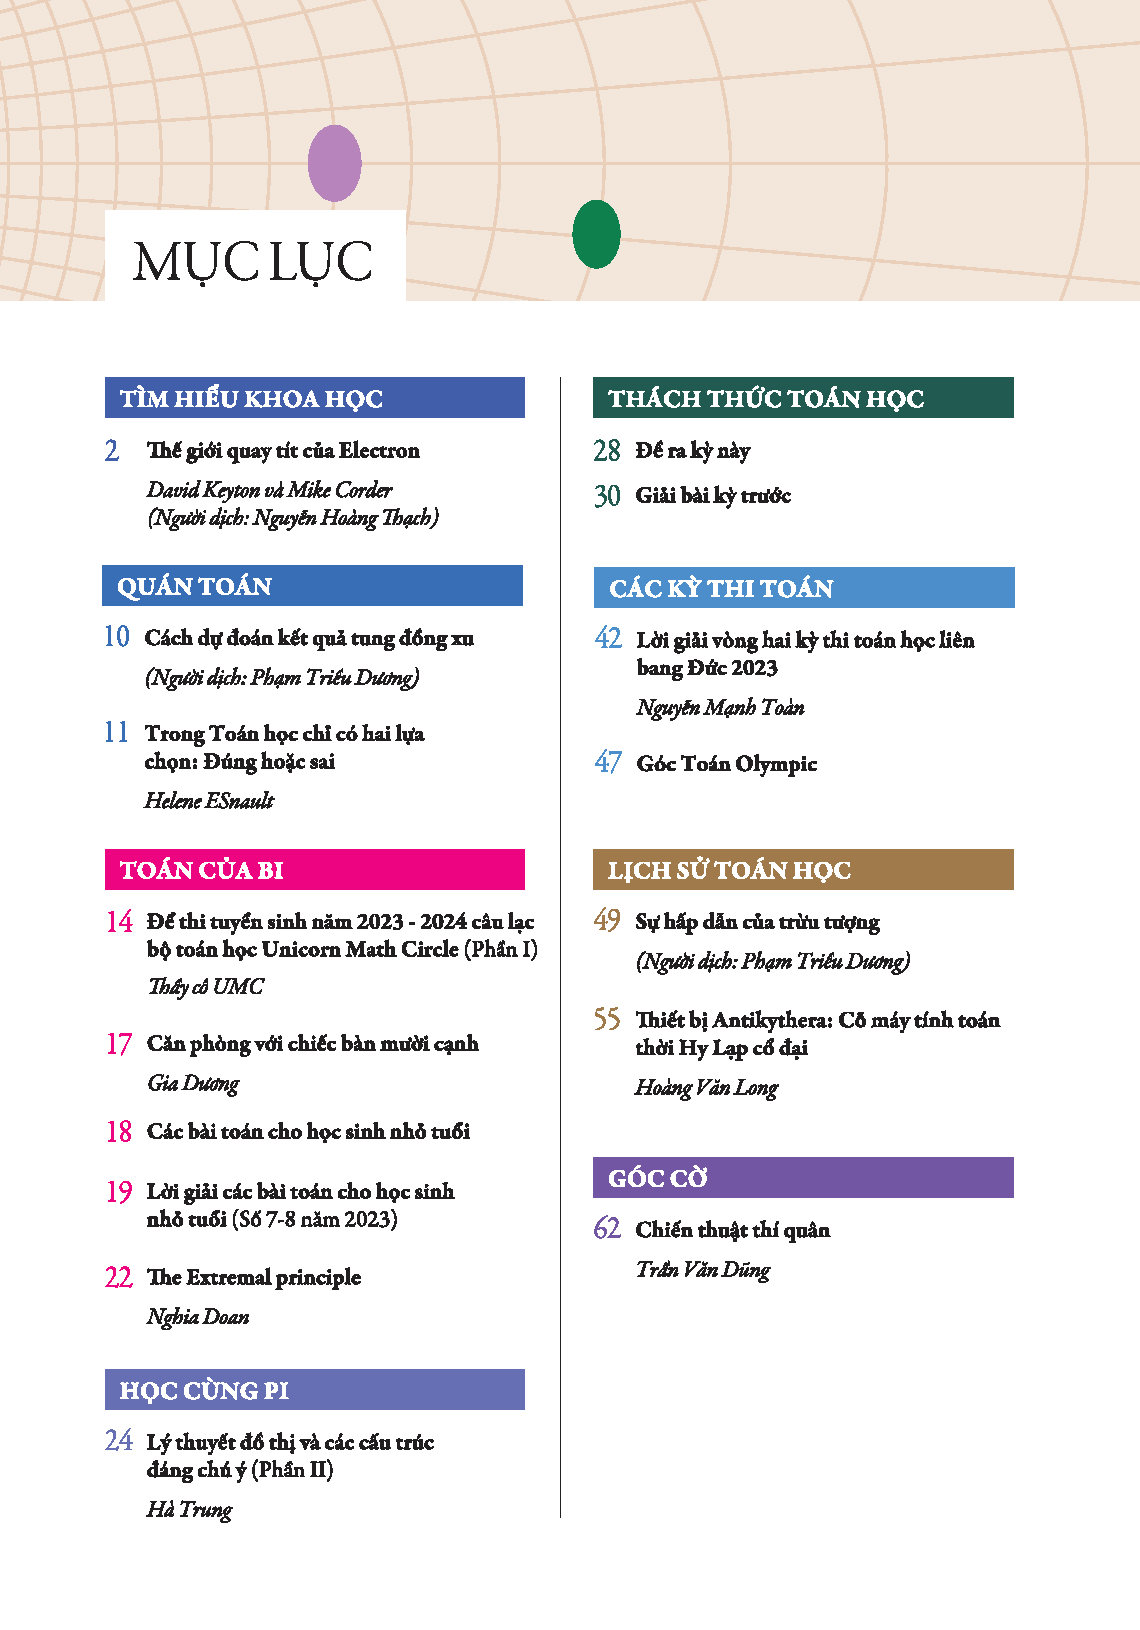
\includegraphics[scale=1]{ML.pdf}}}
%	 \centering
%	 \vspace*{0cm}
%	 \endgroup
%	 \newpage	  
%	 \pagestyle{empty}
%
%	\setcounter{page}{2}
%	\setcounter{figure}{0}
%	\thispagestyle{toanhocvadoisongnone}
\pagestyle{toanhocvadoisong}
\everymath{\color{toanhocdoisong}}
\graphicspath{{../toanhocdoisong/pic/}}
\blfootnote{$^1$\color{toanhocdoisong}Hà Nội.}
\begingroup
\AddToShipoutPicture*{\put(0,616){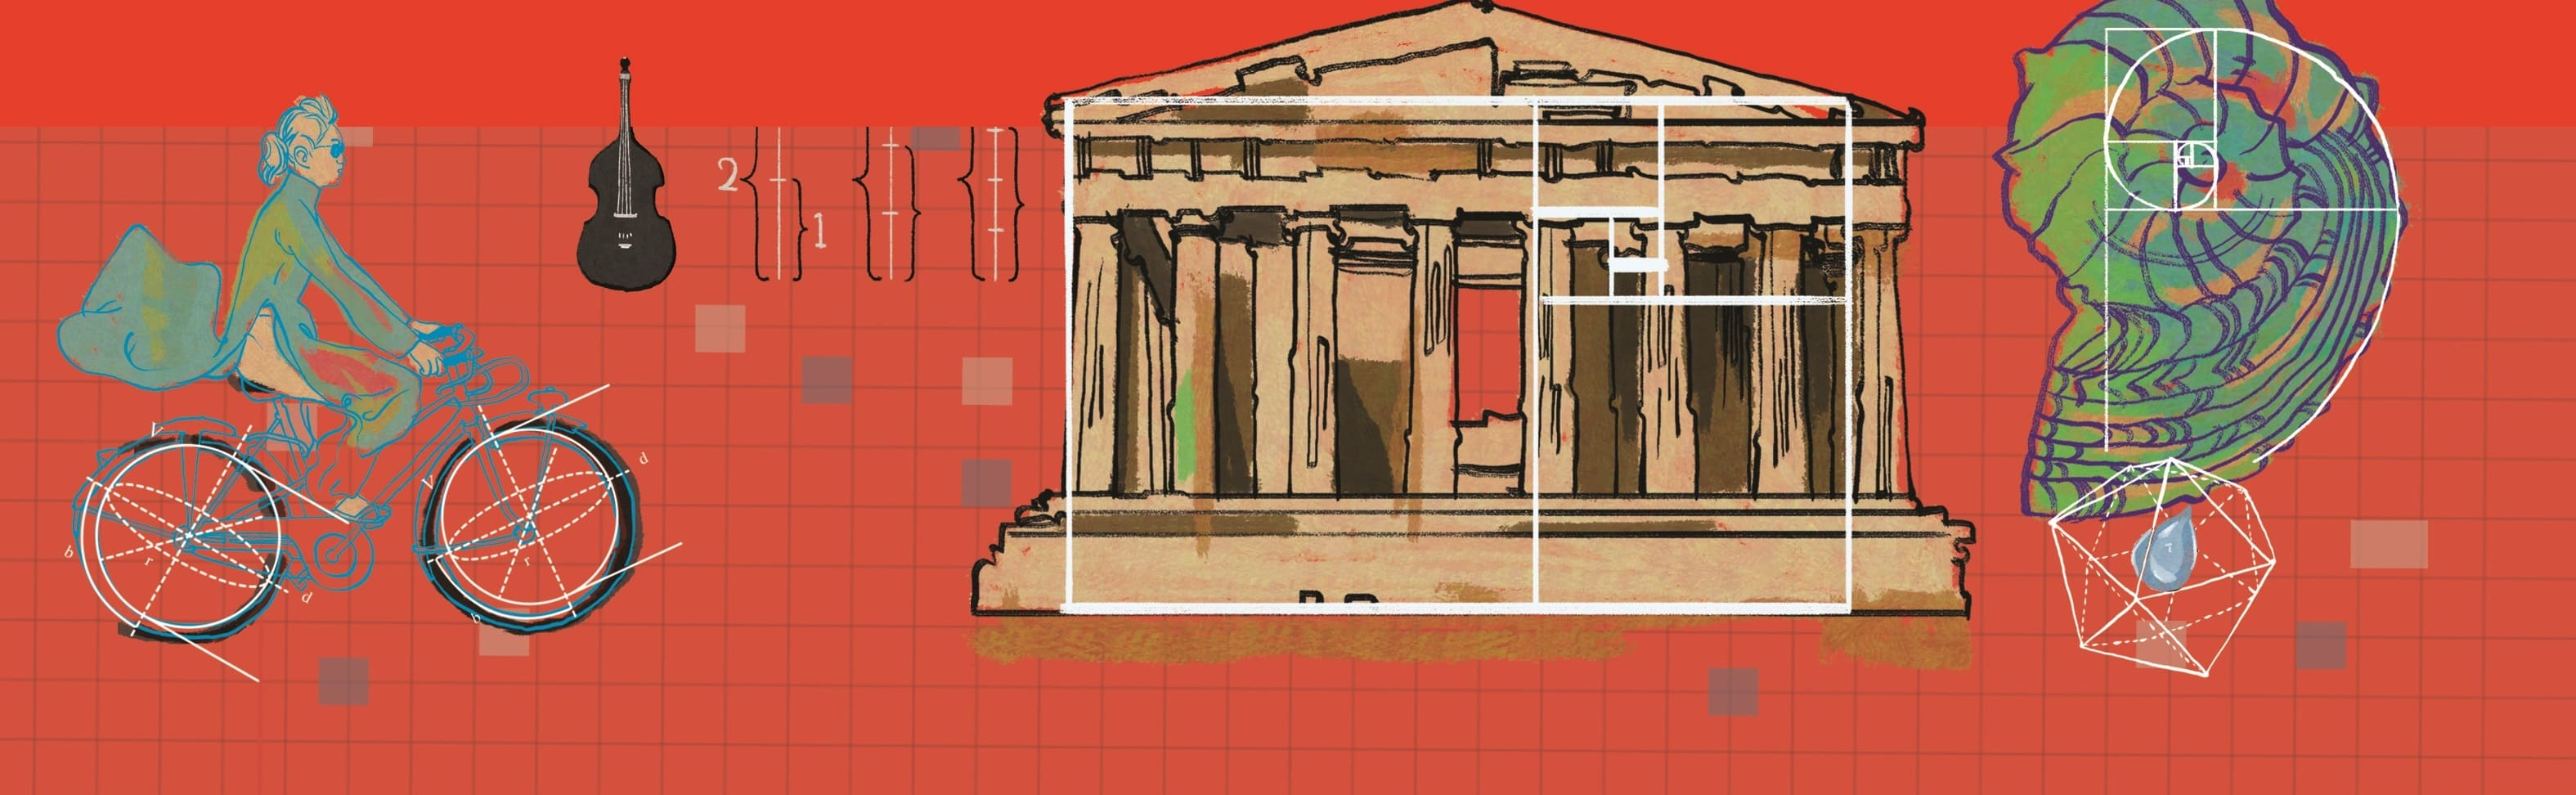
\includegraphics[width=19.3cm]{../bannertoanhocdoisong}}}
\AddToShipoutPicture*{\put(72,524){
\includegraphics[scale=1]{../tieude.pdf}}}
\centering
\endgroup

\vspace*{182pt}

\begin{multicols}{2}
	Có những đường cong tưởng chừng rất xa lạ nhưng lại xuất hiện ở mọi nơi trong đời sống, cả thực lẫn ảo, mà ít người ý thức được sự tồn tại của chúng. Trong bài viết này, chúng ta hãy cùng tìm hiểu về một đường cong như vậy, với tên gọi đường cong Bézier.
	\vskip 0.1cm
	$\pmb{1.}$ \textbf{\color{toanhocdoisong}Bézier, De Casteljau và Bernstein}
	\vskip 0.1cm
	Vào những năm $1950$, với sự phục hồi của nền kinh tế sau chiến tranh thế giới thứ $2$, các hãng xe hơi của Pháp bắt đầu nghiên cứu cho ra các sản phẩm mới mang tính thẩm mỹ cao hơn. Tuy nhiên, phương thức tạo khuôn từ mô hình vật lý ban đầu vẫn không khác giai đoạn trước. Sau khi các nhà thiết kế mỹ thuật tạo ra mô hình nhỏ cho một mẫu xe mới, các bề mặt cong sẽ được phóng đại thủ công bằng cách đo đạc các tọa độ từ mô hình này để vẽ lên các bảng thiết kế kích thước thực. Quy trình tạo khuôn yêu cầu quá trình tỉ mỉ và chi tiết đòi hỏi kinh nghiệm cao từ các kỹ sư thực hiện công đoạn này. Sự thiếu rõ ràng và khả năng xảy ra lỗi cao làm cho việc thiết lập mô hình trong sản xuất có thể lặp đi lặp lại nhiều lần dẫn đến việc tăng chi phí và thời gian.
	\vskip 0.1cm
	Mặt khác, cũng vào giai đoạn này, với sự tài trợ của chính phủ Pháp, các máy tính dạng analog bắt đầu xuất hiện trong nhiều ngành công nghiệp. Chúng được nối trực tiếp với các máy thao tác kim loại trong nhà máy. Các thiết bị này sử dụng đầu vào là những tấm bìa đục lỗ để điều chỉnh đường đi cũng như độ sâu của công cụ cắt. Các đường thẳng, đường tròn, parabola và các hình hình học thông thường đều có thể được đưa vào cho máy thao tác một các chính xác. Tuy nhiên, với các dạng đường cong phức tạp hơn, vẫn chưa có một phương thức phù hợp với công nghệ mới này.
	\begin{figure}[H]
		\vspace*{-5pt}
		\centering
		\captionsetup{labelformat= empty, justification=centering}
		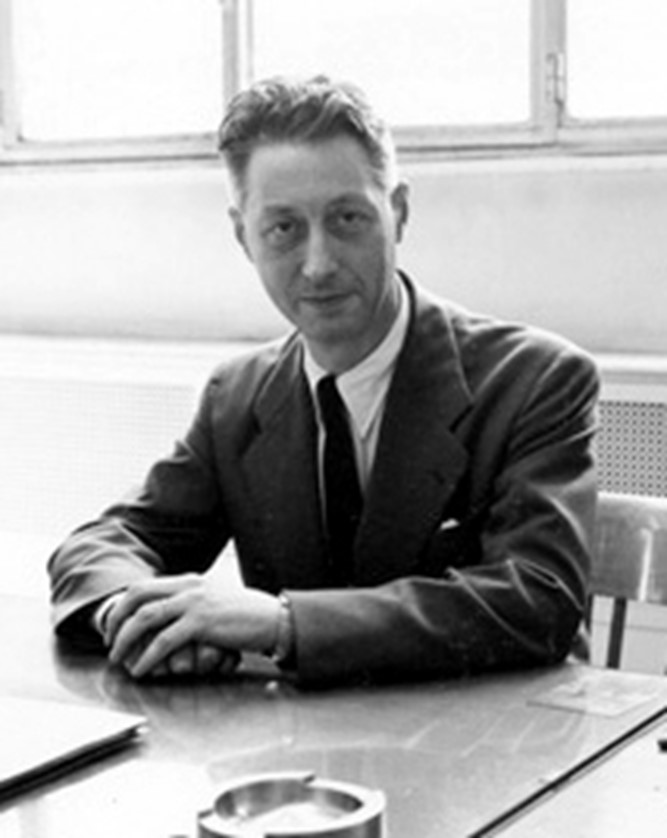
\includegraphics[width= 0.7\linewidth]{1}
		\caption{\small\textit{\color{toanhocdoisong}Pierre Bézier $(1910 - 1999)$.}}
		\vspace*{-10pt}
	\end{figure}	
	Vào đầu những năm $1960$, Pierre Bézier, một kỹ sư tại hãng xe Renault tiến hành tìm phương pháp toán học để giải quyết vấn đề trên. Thay vì dựa vào các kinh nghiệm từ quan sát và thực hành cũng như trí tưởng tượng, việc sản xuất cần được chính xác hóa một cách định lượng. Kết quả từ những nghiên cứu của ông đã cho ra cách xấp xỉ đường cong mà ngày nay được biết đến với tên đường cong Bézier.
	\begin{figure}[H]
		\vspace*{-5pt}
		\centering
		\captionsetup{labelformat= empty, justification=centering}
		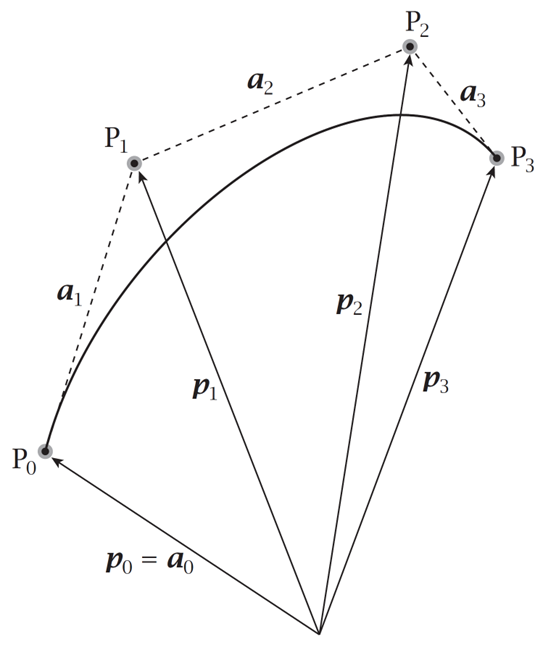
\includegraphics[width= 0.85\linewidth]{2}
		\caption{\small\textit{\color{toanhocdoisong}Hình $1$. Đường cong Bézier được xác định nhờ đường gấp khúc.}}
		\vspace*{-10pt}
	\end{figure}
	Về mặt ý tưởng, đường cong Bézier cho phép ta xấp xỉ một đường cong khác dựa trên một đường gấp khúc. Đồng thời khi điều chỉnh đường gấp khúc này ta cũng có thể thay đổi đường cong được mô tả.
	\vskip 0.1cm
	Ta hãy xét một đường gấp khúc có các đỉnh $P_0,$ $P_1,$ $P_2,$ $P_3$ với các vector tọa độ tương ứng là $\pmb{p_0},$ $\pmb{p_1},$ $\pmb{p_2},$ $\pmb{p_3}$. Các vector của các đoạn gấp khúc sẽ là:
	\begin{align*}
		\pmb{a_1}=\pmb{p_1}-\pmb{p_0},\pmb{a_2}=\pmb{p_2}-\pmb{p_1},\pmb{a_3}=\pmb{p_3}-\pmb{p_2}.
	\end{align*}
	Vector của mỗi điểm trên đường cong sẽ được biểu diễn theo dạng tham số như sau:
	\begin{align*}
		\pmb{r(t)}=\pmb{a_0} + f_{1}(t) \pmb{a_1}+f_{2} (t) \pmb{a_2}+f_{3} (t) \pmb{a_3}
	\end{align*}
	với $\pmb{a_0}= \pmb{p_0}$ và $f_{i}$ là các hàm số của $t$ trong khoảng $[0,1]$.
	\vskip 0.1cm 
	Ta muốn đường cong tham số của ta có hai đầu trùng với đường cong thực tế, tức là:
	\begin{align*}
		\pmb{r(0)}=\pmb{p_0},\pmb{r(1)}=\pmb{p_3}. 
	\end{align*}
	Thay vào biểu thức của $\pmb{r(t)}$, ta được: $f_{1} (0)=f_{2} (0)=f_{3} (0)=0$ và $f_{1} (1)=f_{2}(1)=f_{3}(1)=1$.
	\vskip 0.1cm
	Tiếp theo, ta muốn rằng tiếp tuyến tại $P_0$ và $P_3$ sẽ cùng phương và chiều với các vector $\pmb{a_1}$ và $\pmb{a_3}$. Lấy đạo hàm của $\pmb{r(t)}$ theo $t$ ta có:
	\begin{align*}
		\pmb{r' (t)}=f_{1}' (t) \pmb{a_1}+f_{2}' (t) \pmb{a_3}+f_{3}' (t) \pmb{a_3}.
	\end{align*}
	Điều kiện về tiếp tuyến sẽ cho ta:
	\begin{align*}
		\pmb{r'(0)}&=f_{1}' (0) \pmb{a_1}+f_{2}' (0) \pmb{a_2}+f_{3}'(0) \pmb{a_3}\\
		&=k\pmb{a_1}\\
		\pmb{r'(1)}&=f_{1}' (1) \pmb{a_1}+f_{2}' (1) \pmb{a_2}+f_{3}'(1) \pmb{a_3}\\
		&=k\pmb{a_3}
	\end{align*}
	tương đương với $f_{2}' (0)=f_{3}' (0) = f_{1}' (1)=f_{2}' (1)=0$.
	\vskip 0.1cm
	Ta cũng muốn rằng đạo hàm cấp hai $\pmb{r''(t)}=f_{1}'' (t) \pmb{a_1}+f_{2}'' (t) \pmb{a_2}+f_{3}'' (t) \pmb{a_3}$ chỉ phụ thuộc vào $\pmb{a_1,a_2}$ tại $P_0$ và ${\pmb{a_2,a_3}}$ tại $P_3$. Để thỏa mãn điều kiện này $f_{3}'' (0)=f_{1}'' (1)=0$.
	\vskip 0.1cm
	Bézier chọn các hàm $f$ là các hàm đa thức bậc $3$:
	\begin{align*}
		f_{i}(t)=\alpha_i t^3 + \beta_i t^2+\gamma_i t + \delta_i,1 \le i \le 3.
	\end{align*}
	Thay vào các điều kiện ở trên và giải hệ phương trình tuyến tính ta được:
	\begin{align*}
		&f_{1} (t)=t^3-3t^2+3t\\
		&f_{2} (t)=-2t^3+3t^2\\
		&f_{3} (t)=t^3.
	\end{align*}
	Khi đó:
	\begin{align*}
		\pmb{r(t)}=\,&\pmb{a_0}+(t^3-3t^2+3t) \pmb{a_1}\\
		&+(-2t^3+3t^2 ) \pmb{a_2}+t^3 \pmb{a_3}, \,\,\,0 \le t \le 1.
	\end{align*}
	Phương trình đường cong theo tham số này cho phép ta điều chỉnh hình dạng của đường cong bằng cách thay đổi các vector $\pmb{a_0},$ $\pmb{a_1},$ $\pmb{a_2},$ $\pmb{a_3}$. Đường cong Bézier cũng có thể được mở rộng bằng cách sử dụng các đa thức với bậc lớn hơn $3$ nhưng trong thực tế việc này là không cần thiết. Thậm chí trong một số trường hợp đơn giản hơn, người ta chỉ dùng đường cong Bézier bậc $2$:
	\begin{align*}
		\pmb{r(t)}=\pmb{a_0}+(-t^2+2t) \pmb{a_1}+t^2 \pmb{a_2}.
	\end{align*}
	Bézier đã phát triển phương pháp mô tả đường cong trên của mình thành hệ thống UNISURF phục vụ cho công việc sản xuất ô tô. Thay vì những mô tả phức tạp, với mỗi đoạn cong, ta chỉ cần lưu tọa độ của $4$ điểm mà thôi, giúp cho việc số hóa đường cong trở nên đơn giản hơn rất nhiều. Tuy nhiên phải đến năm $1966$, khi Renault ký thỏa thuận hợp tác với một hãng xe nổi tiếng khác là Peugeot, phần mềm này mới bắt đầu được các kỹ sư sử dụng. Năm $1968$ đánh dấu sự ra đời của mẫu xe Peugeot $204$, chiếc xe đầu tiên có toàn bộ vỏ xe được xây dựng sử dụng phần mềm máy tính. Sự kiện này có ý nghĩa quan trọng là cột mốc bắt đầu vai trò của CAD (Computer Aided Design -- thiết kế có máy tính hỗ trợ) trong các ngành công nghiệp.
	\begin{figure}[H]
		\vspace*{-5pt}
		\centering
		\captionsetup{labelformat= empty, justification=centering}
		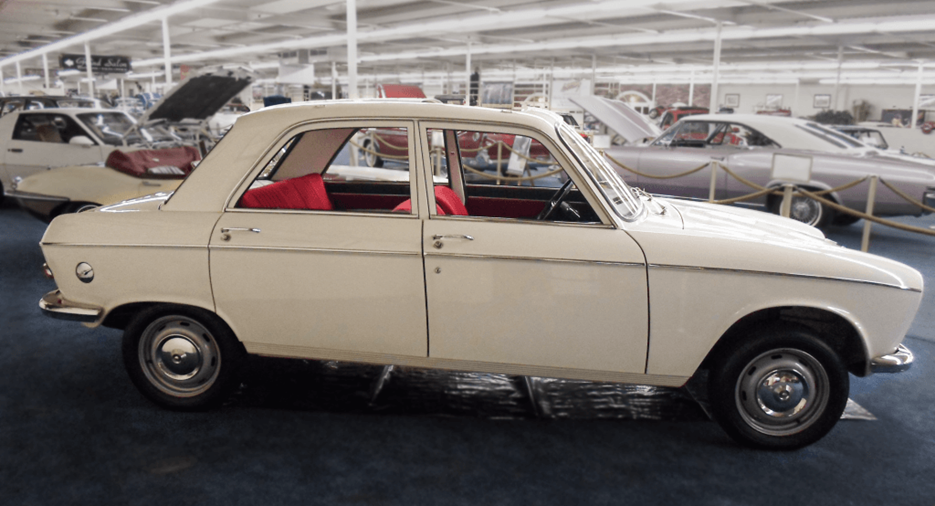
\includegraphics[width= 1\linewidth]{3}
		\caption{\small\textit{\color{toanhocdoisong}Hình $2$. Mẫu xe Peugeot $204$ ra đời năm $1968$.}}
		\vspace*{-10pt}
	\end{figure}
	\vskip 0.1cm
	\PIbox{Bézier từng kể lại rằng, một nhân tố giúp ông thuyết phục thành công mọi người sử dụng phương pháp của mình là việc gán các kết quả toán học cho giáo sư Onésimer Durand, một nhân vật giả tưởng ông tự bịa ra. Điều này giúp mọi người cảm thấy tin tưởng nhiều hơn vào các kết quả của Bézier. Nhiều thập kỷ sau, Bézier khi đi giảng bài vẫn được hỏi rằng giáo sư Durand là ai và giảng dạy ở đâu!}
	\vskip 0.1cm
	Về mặt lịch sử, đường cong Bézier đã được khám phá trước đó không lâu bởi De Casteljau, một kỹ sư ở hãng xe Citroën cũng của Pháp. Công trình này được ông công bố nội bộ năm $1963$. Tuy nhiên, do hãng coi đây là một bí mật công nghiệp, nó đã không được công bố ra bên ngoài cho đến tận năm $1975$.
	\vskip 0.1cm
	Thay vì sử dụng các vector như Bézier, De Casteljau xấp xỉ các đường cong dựa trên các điểm cực. Giả sử một đường cong có hai đầu ở $P_0$ và $P_2$. Một điểm $P_1$ được sử dụng để làm điểm điều khiển. Trên $P_0 P_1$ lấy điểm $Q_0$ sao cho $\dfrac{P_0Q_0}{P_0P_1} = k$ Tương tự, trên $P_1 P_2$ lấy điểm $Q_1$ sao cho $\frac{P_1 Q_1}{P_1 P_2}$ cũng bằng $k$. Trên $Q_0 Q_1$ ta lại lấy điểm $R$ sao cho $\dfrac{Q_0 R}{Q_0 Q_1} = k$. Từ tọa độ của $P_0,$ $P_1,$ $P_2$ có thể dễ dàng tính được tọa độ của $Q_0,$ $Q_1$ và $R$ bằng các công thức hình học giải tích. $R$ sẽ là một điểm nằm trên đường cong ta cần mô tả. Tiếp đó, các bộ ba điểm $P_0,$ $Q_0,$ $R$ và $R,$ $Q_1,$ $P_2$ lại cho ta $2$ điểm tiếp theo thuộc đường cong. Lặp lại quá trình này cho đến khi được số lượng điểm nằm trên đường cong đủ dày đặc, ta có thể nối chúng bằng các đoạn thẳng để xấp xỉ đường cong. Bạn đọc có thể tự chứng minh để thấy rằng các điểm được xác định bằng thuật toán trên nằm trên một đường cong Bézier bậc $2$. Khi ta di chuyển các điểm $P_0,$ $P_1$  và $P_2$, ta có thể thay đổi được hình dạng của đường cong theo ý muốn.
	\begin{figure}[H]
		\vspace*{-5pt}
		\centering
		\captionsetup{labelformat= empty, justification=centering}
		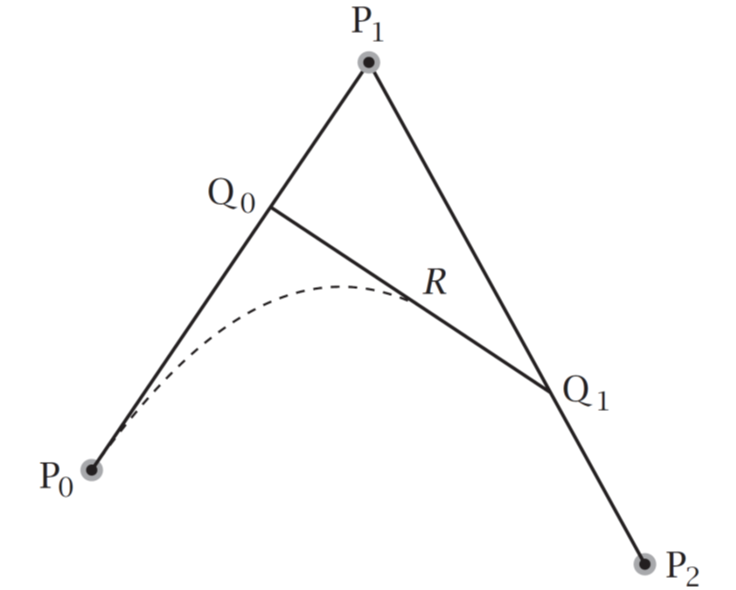
\includegraphics[width= 0.9\linewidth]{4}
		\caption{\small\textit{\color{toanhocdoisong}Hình $3$. Thuật toán De Casteljau.}}
		\vspace*{-5pt}
	\end{figure}
	Do De Casteljau phát hiện ra trước nhưng không được đặt tên cho đường cong, người ta đã bù đắp bằng cách đặt tên thuật toán tách đường cong trên là thuật toán De Casteljau. Thuật toán De Casteljau với $k=0,5$ có thể được cài đặt hiệu quả trên các máy tính điện tử do việc chia một số cho $2$ là rất dễ dàng với hệ cơ số nhị phân.
	\vskip 0.1cm
	Đường cong Bézier còn có thể được mở rộng cho không gian $3$ chiều. Khi đó ta sẽ có mặt cong Bézier.
	\begin{figure}[H]
		\vspace*{-5pt}
		\centering
		\captionsetup{labelformat= empty, justification=centering}
		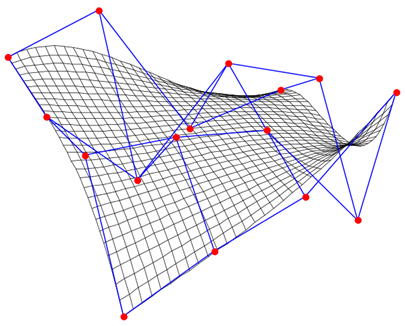
\includegraphics[width= 0.9\linewidth]{5}
		\caption{\small\textit{\color{toanhocdoisong}Hình $4$. Mặt cong Bézier trong không gian $3$ chiều.}}
		\vspace*{-10pt}
	\end{figure}
	\PIbox{
	\textbf{\color{toanhocdoisong}Đường cong Bézier và font chữ máy tính}
	\vskip 0.1cm
	Việc hiển thị các font chữ khi soạn thảo văn bản trên máy tính cũng như khi in ấn từ máy tính là một vấn đề tưởng đơn giản nhưng lại phức tạp. Vào thời ban đầu của máy tính, các font được lưu dưới dạng bitmap, với các kích cỡ font khác nhau, ta cần các bitmap với độ phân giải khác nhau, rất tốn kém và không hiệu quả.
	\vskip 0.1cm
	Đến năm $1985$, John Warnock, người sáng lập ra công ty Adobe, đã đưa ra một giải pháp mới. Ông đã phát triển một ngôn ngữ lập trình với tên gọi PostScript để có thể xây dựng trang văn bản dựa trên các cấu trúc toán học. Trong đó, các font chữ được lưu dưới dạng font vector, dạng font mà sau này cả Apple lẫn Microsoft đều sử dụng cho các thế hệ font chữ sau này. Với những thành phần của font chữ là dạng} 
	\vskip 0.1cm
	\PIbox{
	 đường cong, đường cong Bézier bậc $3$ được sử dụng để lưu trữ chúng trong máy tính. Ví dụ như với chữ O ở bên dưới, với mỗi đoạn cong giữa hai điểm được đánh dấu liên tiếp, người ta cần lưu $4$ tọa độ gồm tọa độ của hai điểm được đánh dấu và tọa độ của hai điểm còn lại để biểu diễn đoạn cong này dưới dạng đường cong Bézier.
	\vskip 0.1cm
	Đường cong Bézier cũng trở thành công cụ chính trong Illustrator, một phần mềm khác của Adobe. Thay vì các thao tác phức tạp, những người thiết kế đồ họa chỉ cần nhấn chuột vài lần để tạo một đường cong trong phần mềm. Việc này đã thay đổi hoàn toàn ngành công nghiệp thiết kế đồ họa.
	\begin{figure}[H]
		\vspace*{-5pt}
		\centering
		\captionsetup{labelformat= empty, justification=centering}
		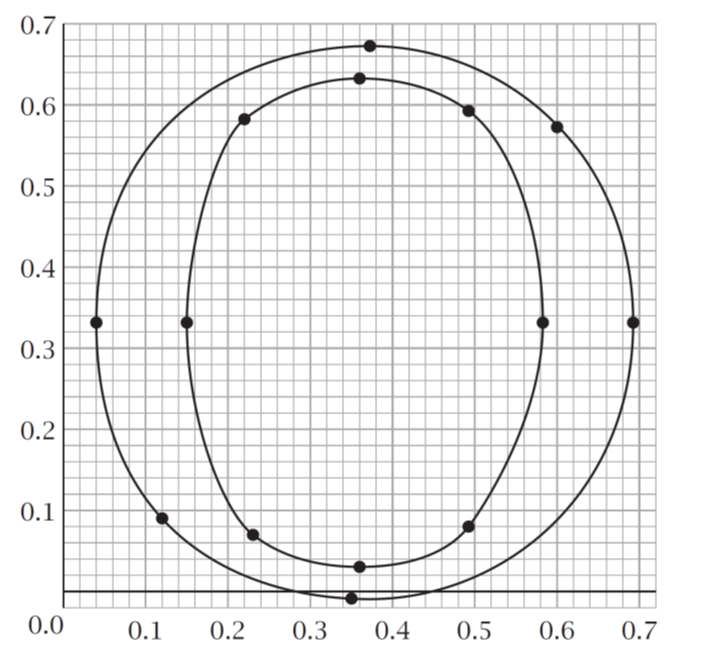
\includegraphics[width= 1\linewidth]{6}
		%		\caption{\small\textit{\color{}}}
		\vspace*{-15pt}
	\end{figure}}
	\vskip 0.2cm
	$\pmb2.$ \textbf{\color{toanhocdoisong}Sơ lược về đa thức Bernstein}
	\vskip 0.1cm
	Nếu viết đường cong Bézier bậc $3$ theo tọa độ của các điểm xác định nó (thay vì các vector $\pmb{a_i}$), ta được phương trình:
	\begin{align*}
		\pmb{r(t)}= &(1-t)^3 \pmb{p_0}+3t(1-t)^2 \pmb{p_1}\\
		&+3t^2 (1-t) \pmb{p_2}+t^3 \pmb{p_3}.
	\end{align*}
	Các đa thức $(1-t)^3,3t(1-t)^2,3t^2 (1-t)$ và $t^3$ có thể được coi là trọng số ứng với tọa độ của mỗi điểm trong biểu diễn của đường cong. Bạn đọc với trực giác toán học tốt sẽ nhận ngay thấy chúng là các đa thức thành phần khi ta tiến hành khai triển $\left(t+(1-t)\right)^3$.
	\vskip 0.1cm
	Các đa thức dạng này còn được gọi là các đa thức Bernstein:
	\begin{align*}
		B_i^n (t)&= \left(\!\!\begin{array}{l}
			n\\
			i
		\end{array}\!\!\right)t^i (1-t)^{n-i},\\
	&1 \le i \le n,0 \le t \le 1.
	\end{align*}
	Các đa thức Bernstein được suy ra từ biến đổi sau:
	\begin{align*}
		1 &= 1^n = \left(t + (1-t)\right) \\
		&= \sum\limits_{i = 0}^n {\left( \begin{array}{l}
				n\\
				i
			\end{array} \right){t^i}{{(1 - t)}^{n - i}} = } \sum\limits_{i = 0}^n {B_i^n(t).}
	\end{align*}
	Chúng được đặt tên theo nhà toán học Liên Xô Sergei Bernstein. Ông là một nhà toán học có nhiều đóng góp về vấn đề xấp xỉ hàm số. Ta luôn có thể biểu diễn một đa thức bất kỳ dưới dạng tổ hợp tuyến tính của các đa thức Bernstein. Theo thuật ngữ trong đại số tuyến tính, các đa thức này tạo thành một cơ sở của không gian vector các đa thức.
	\begin{figure}[H]
		\vspace*{-5pt}
		\centering
		\captionsetup{labelformat= empty, justification=centering}
		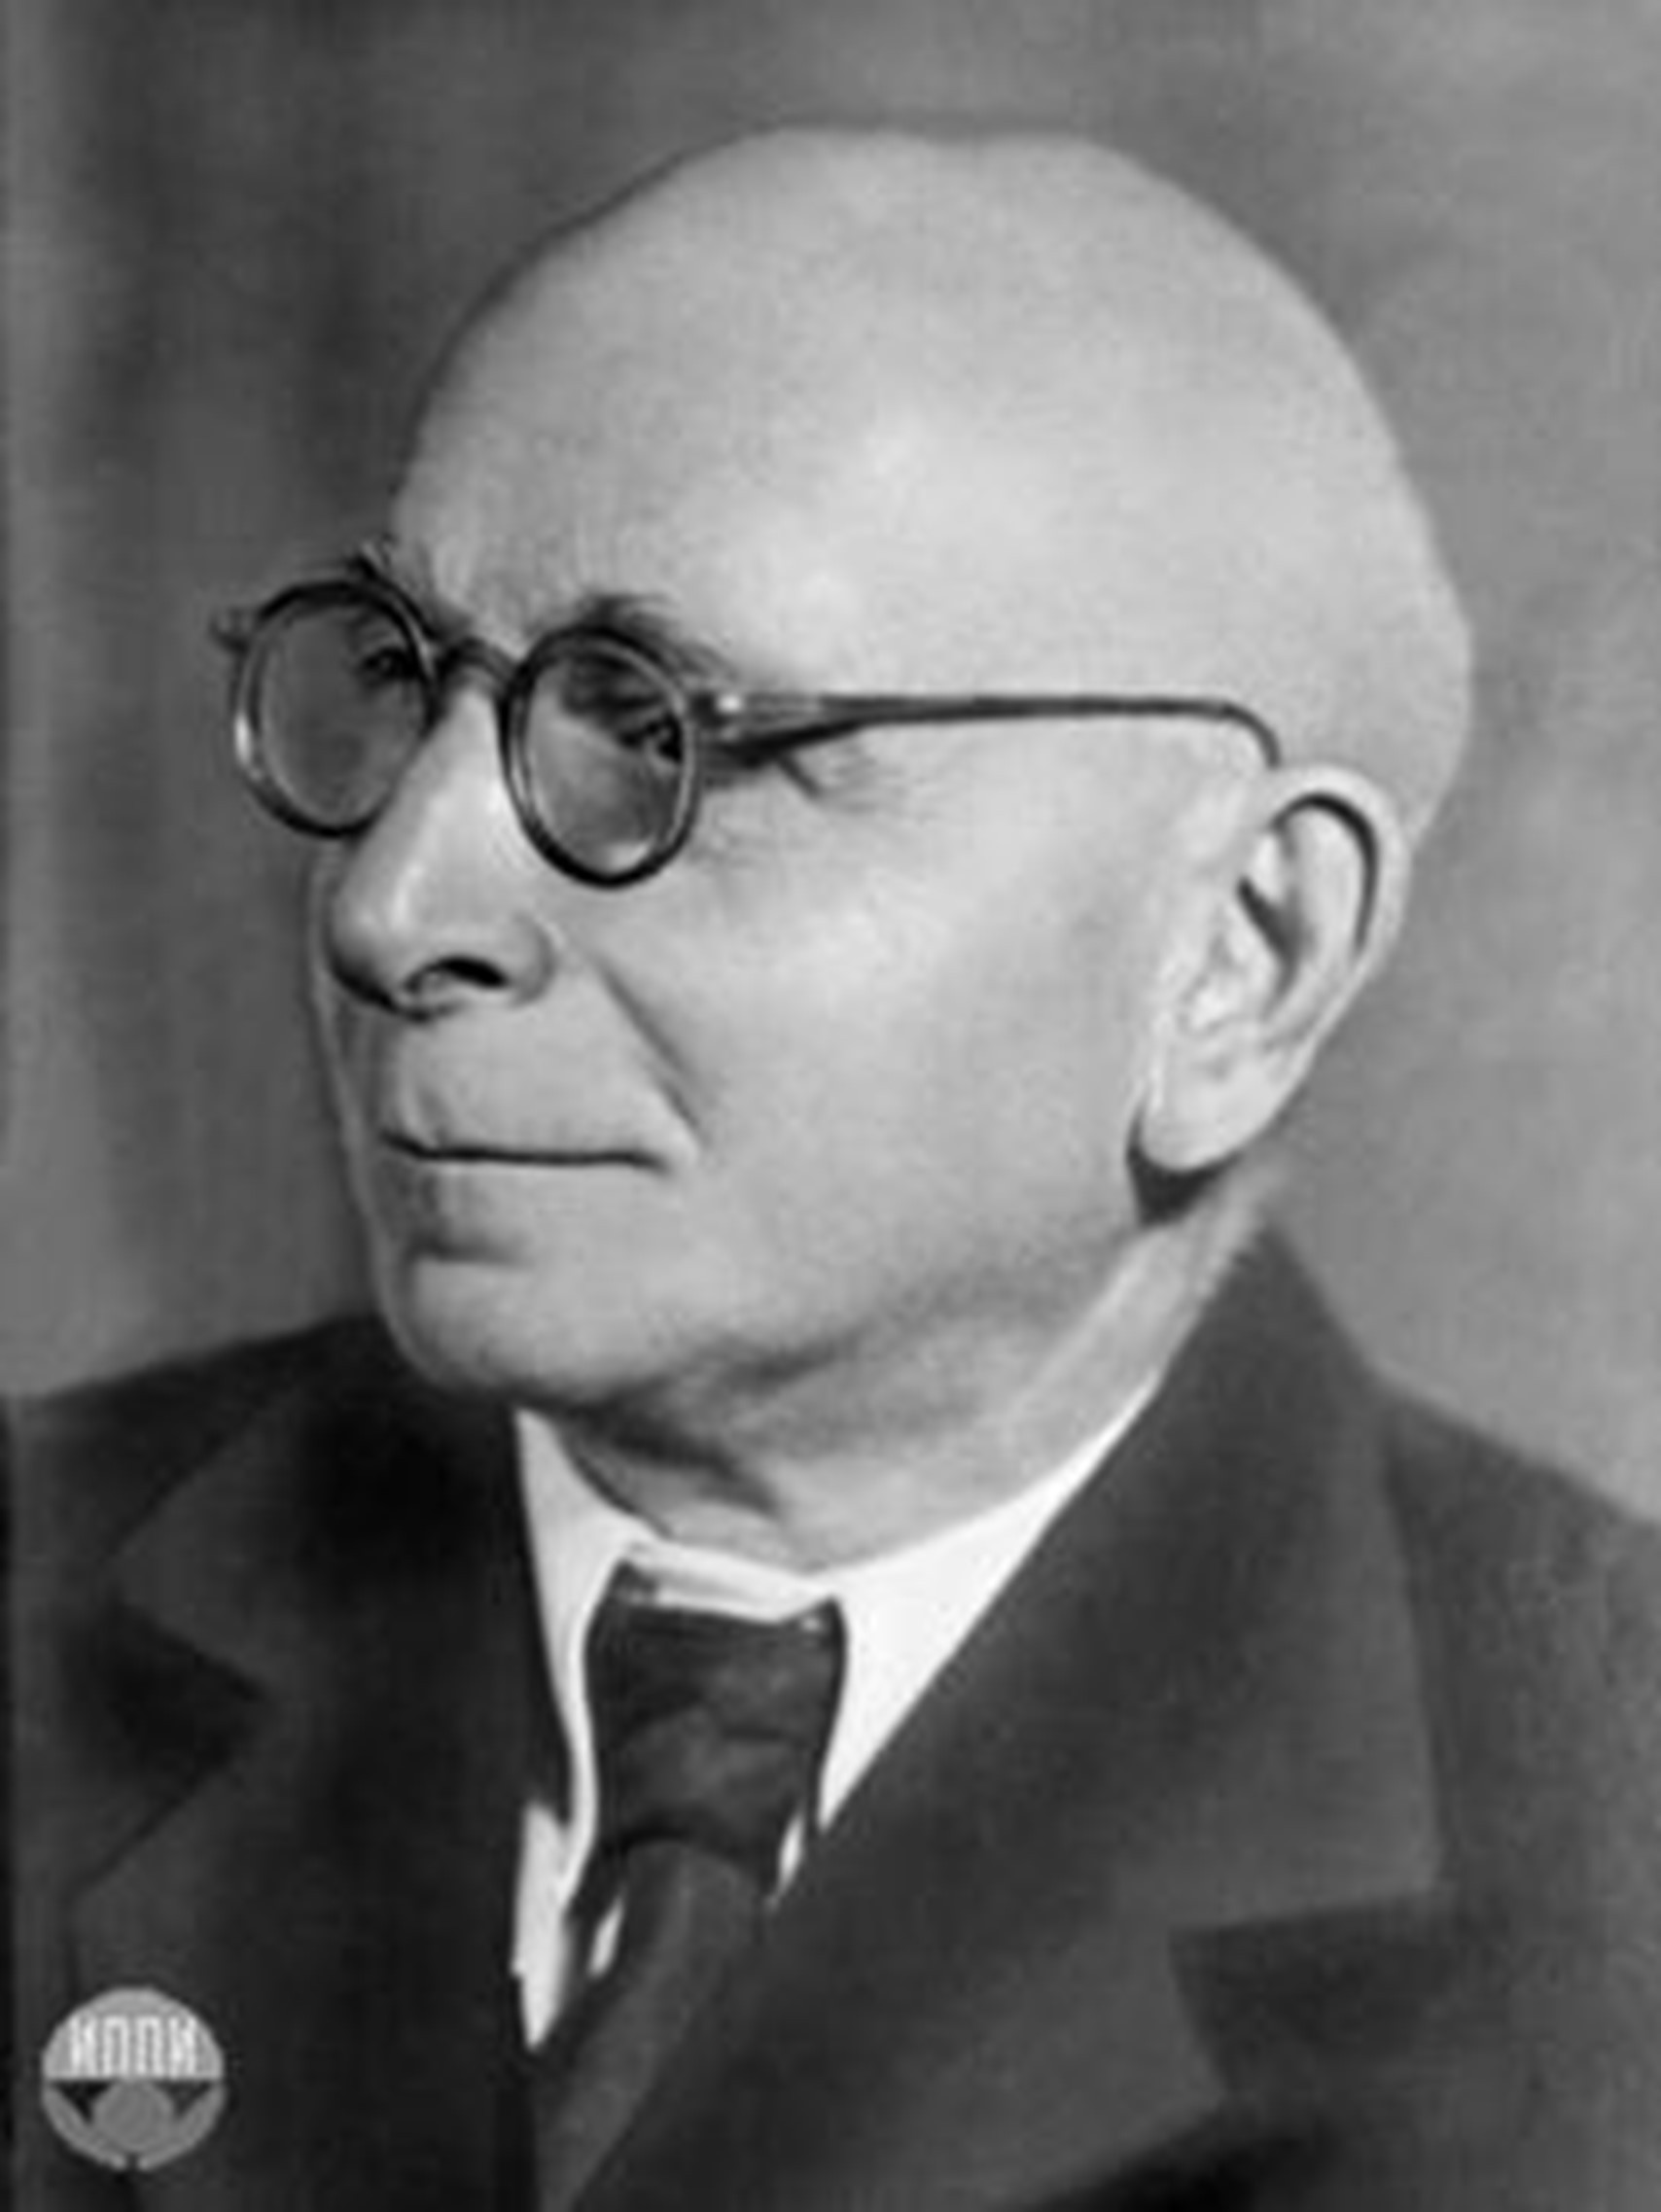
\includegraphics[width= 0.6\linewidth]{7}
		\caption{\small\textit{\color{toanhocdoisong}Sergei Natanovich Bernstein $(1880-1968)$.}}
		\vspace*{-10pt}
	\end{figure}
	Bernstein đã sử dụng các đa thức mang tên mình để chứng minh định lý xấp xỉ Weierstrass: ``các đa thức với bậc đủ cao có thể xấp xỉ bất cứ hàm số liên tục nào trên một khoảng hữu hạn''. Ông đã chứng minh rằng:
	\begin{align*}
		\mathop {\lim }\limits_{n \to \infty } {B_n}(f,t) = f(t)
	\end{align*}
	với $B_n(f,t) = \sum\limits_{i = 0}^n {f\left( {\frac{i}{n}} \right)B_i^n(t)}$ trên khoảng $[0,1]$ (chứng minh này được trình bày ở phần phụ lục). Do biến đổi $t \to \dfrac{t-a}{b-a}$ cũng biến đổi $[a,b] \to [0,1]$ nên định lý được chứng minh.
	\vskip 0.1cm
	Tuy rằng tốc độ hội tụ của hàm đa thức $B_n$ rất chậm, trong thực tế các đa thức Bernstein bậc $2$ hoặc bậc $3$ thường đã đủ để thỏa mãn các nhu cầu ứng dụng, ví dụ như trường hợp đường cong Bézier. Bản thân De Casteljau cũng đã tiến hành xây dựng nghiên cứu của mình dựa trên lý thuyết về đa thức Bernstein. Có thể thấy rằng những nghiên cứu toán học tưởng như trừu tượng lại nhiều lúc tạo cơ sở cho những ứng dụng thực tiễn đầy thú vị.
	\vskip 0.1cm
	\PIbox{\textbf{\color{toanhocdoisong}Hàm spline}
	\vskip 0.1cm
	Trước kia, người ta dùng thuật ngữ \textit{spline} để gọi tên thanh gỗ được uốn cong bằng cách kẹp cố định một số điểm. Cách làm này giúp tạo ra đường cong được uốn tự nhiên trong quá trình đóng tàu. Trong toán học, các hàm số có dạng đa thức trên từng đoạn được gọi là các hàm spline. Những đường cong dùng để xấp xỉ sử dụng những hàm spline được gọi là các đường cong spline, bao gồm đường cong Bézier và những đường cong được phát triển sau này dựa trên nó như B--spline, NURB, ... Những đường cong này hiện nay được ứng dụng rộng rãi trong các lĩnh vực công nghiệp như sản xuất máy bay, ô tô, thời trang, ... cũng như trong các lĩnh vực đồ họa máy tính và kiến trúc.
	\begin{figure}[H]
		\vspace*{-5pt}
		\centering
		\captionsetup{labelformat= empty, justification=centering}
		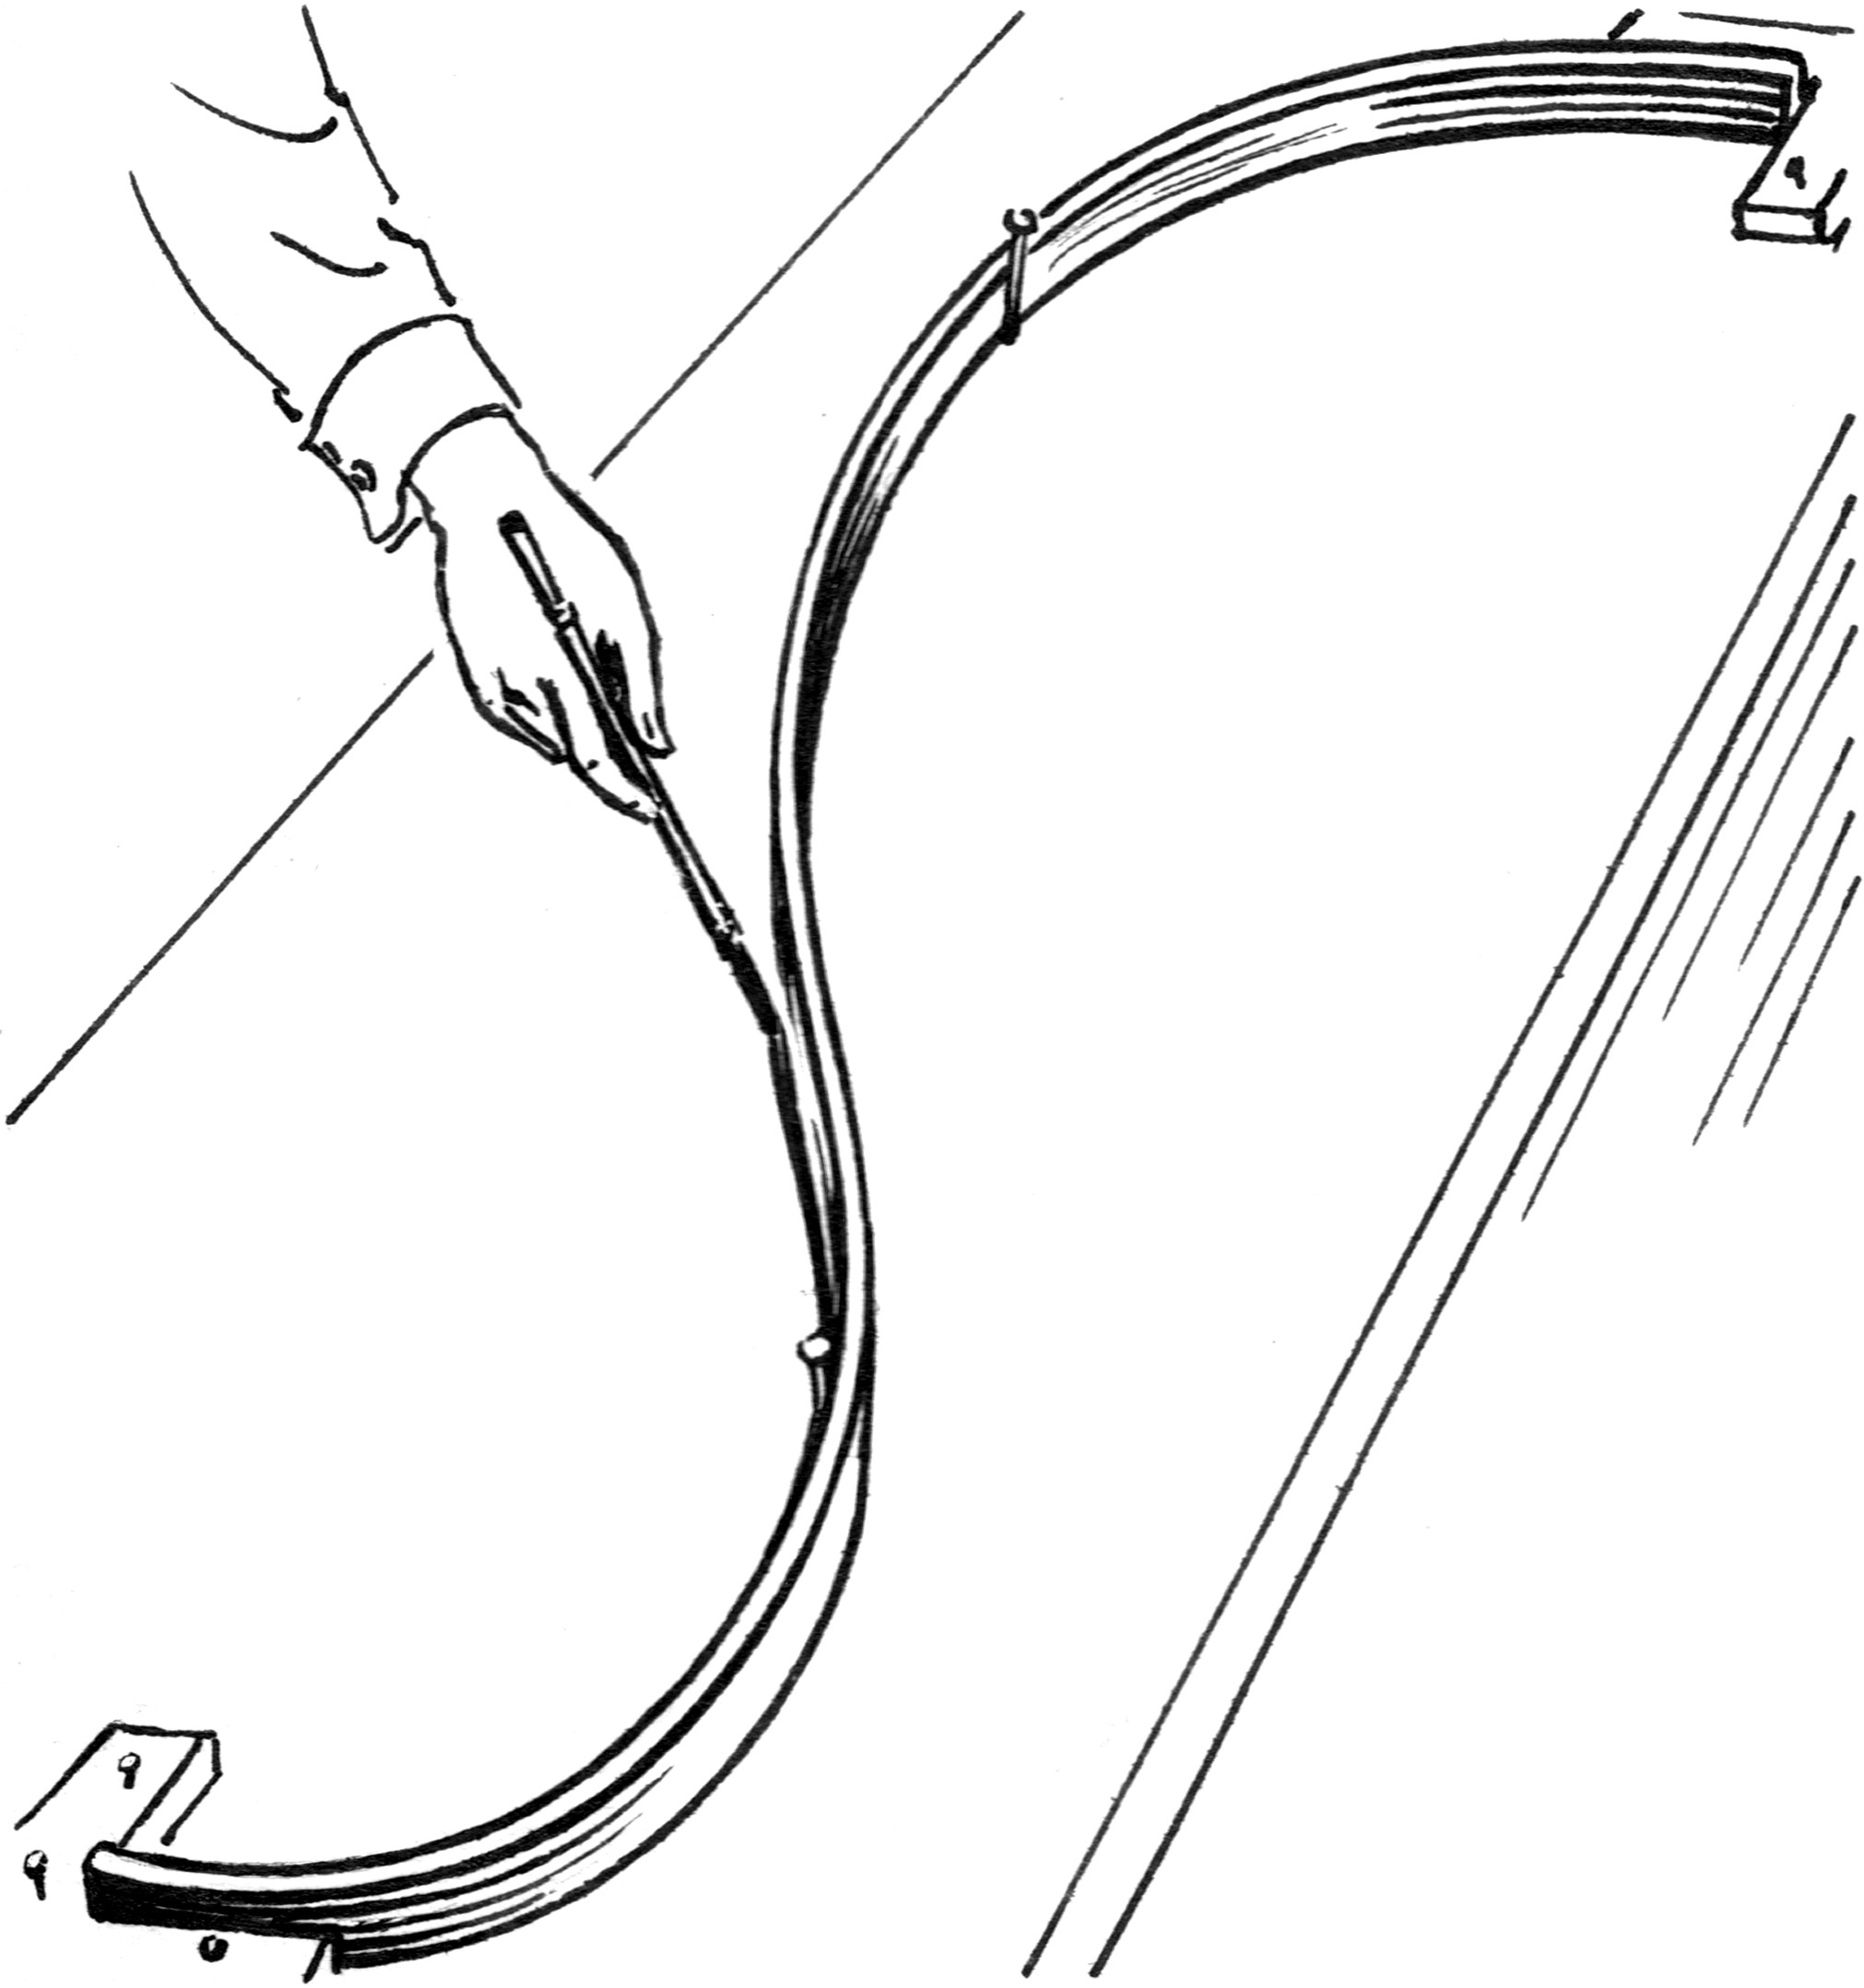
\includegraphics[width= 0.65\linewidth]{8}
		\caption{\small\textit{\color{toanhocdoisong}Cách làm thanh spline khi đóng tàu.}}
%		\vspace*{-10pt}
	\end{figure}}
	$\pmb3.$ \textbf{\color{toanhocdoisong}Vẽ đường cong Bézier bằng quỹ tích trong GeoGebra}
	\vskip 0.1cm
	Ta có thể vẽ đường cong Bézier bằng cách nhập phương trình tham số một cách trực tiếp. Tuy nhiên, việc vẽ bằng quỹ tích sẽ mang tính trực quan hơn. Để vẽ đường cong này theo quỹ tích, ta sử dụng cách mô tả của De Casteljau và cho hệ số $k$ thay đổi trong khoảng $[0,1]$. Khi $k=0$, $R$ trùng với $P_0$, còn khi $k=1$, $R$ trùng với $P_1$. Quỹ tích của $R$ chính là đường cong Bézier.
	\vskip 0.1cm
	Trong GeoGebra, trước hết ta chọn các điểm $P_0$, $P_1$ và $P_2$ trong mặt phẳng rồi nối các đoạn thẳng $P_0 P_1$ và $P_1 P_2$.
	\begin{align*}
		&d_1= segment (P_0,P_1)\\
		&d_2= segment (P_1,P_2)
	\end{align*}
	\begin{figure}[H]
		\vspace*{-5pt}
		\centering
		\captionsetup{labelformat= empty, justification=centering}
		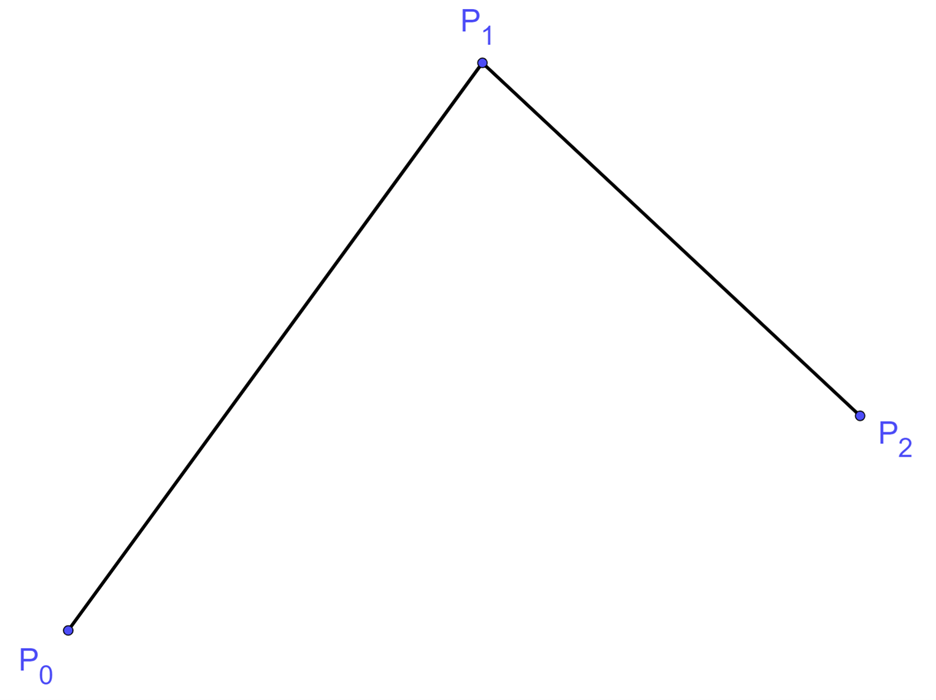
\includegraphics[width= 0.8\linewidth]{9}
		\caption{\small\textit{\color{toanhocdoisong}Hình $5$. Chọn $3$ điểm trong mặt phẳng để xác định đường cong Bézier bậc $2$.}}
		\vspace*{-10pt}
	\end{figure}
	Ta cho tham số $k$ chạy từ $0$ đến $1$:
	\begin{align*}
		k = slider (0,1).
	\end{align*}
	Để xác định các điểm $Q_0$ và $Q_1$, thay vì dùng công thức dạng vector, ta có thể sử dụng giao điểm của đường tròn và đoạn thẳng:
	\begin{align*}
		&Q_0=intersect\left(\text{circle} (P_0,d_1*k),d_1\right)\\
		&Q_1=intersect\left(\text{circle} (P_1,d_2*k),d_2\right)
	\end{align*}
	Điểm $R$ cũng được xác định tương tự:
	\begin{align*}
		&d_3=segment(Q_0,Q_1 )\\
		&R=intersect\left(\text{circle} (Q_0,d_3*k),d_3\right).
	\end{align*}
	Ta ấn chuột phải vào điểm $R$ và chọn ``Show trace''. Khi đó, cho thanh trượt của $k$ di chuyển từ $0$ đến $1$, quỹ tích của $R$ sẽ cho ta đường cong Bézier bậc $2$ (bạn đọc có thể thử chứng minh bằng hình học giải tích rằng nó chính là đường cong này).
	\begin{figure}[H]
		\vspace*{-5pt}
		\centering
		\captionsetup{labelformat= empty, justification=centering}
		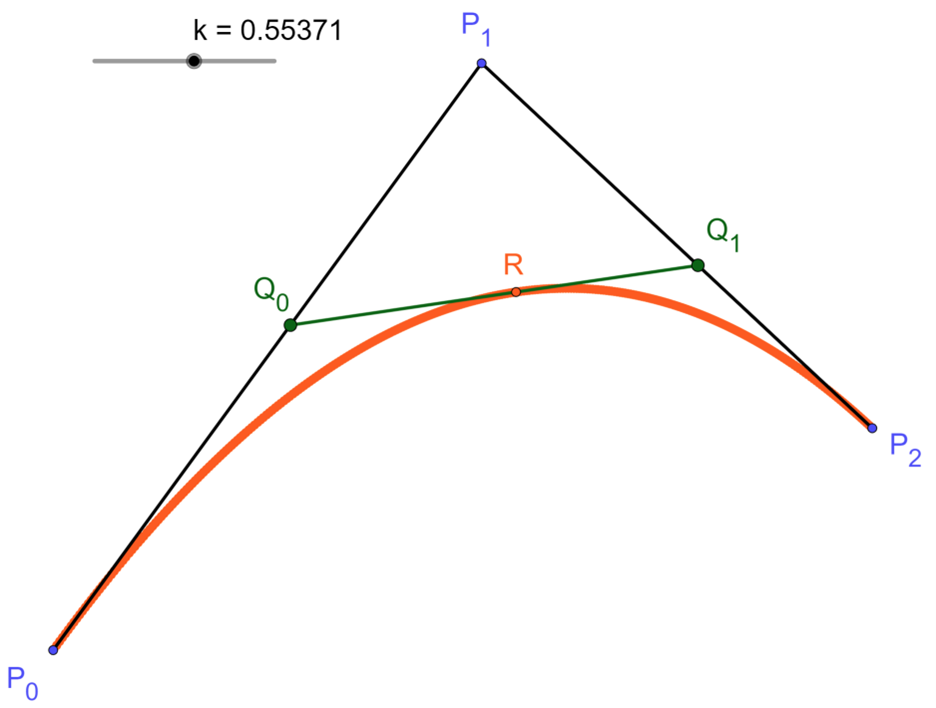
\includegraphics[width= 0.8\linewidth]{10}
		\caption{\small\textit{\color{toanhocdoisong}Hình $6$. Đường cong Bézier bậc $2$ dưới dạng quỹ tích trong GeoGebra.}}
		\vspace*{-10pt}
	\end{figure}
	Với đường cong Bézier bậc $3$, ta sẽ có $4$ điểm $P_0,P_1,P_2$ và $P_3$. Để tiến hành dựng đường cong, ta xác định các điểm $Q_0,Q_1$ và $Q_2$ sao cho $\dfrac{P_0 Q_0}{P_0 P_1}= \dfrac{P_1 Q_1}{P_1 P_2}= \dfrac{P_2 Q_2}{P_2 P_3} =k$. Từ $3$ điểm này, ta lại tiếp tục tìm các điểm $R_1$, $R_2$ và $S$ sao cho $\dfrac{Q_0 R_1}{Q_0 Q_1} = \dfrac{Q_1 R_2}{Q_1 Q_2}= \dfrac{R_1 S}{R_1 R_2}=k$. Quỹ tích của $S$ chính là đường cong cần dựng.
	\begin{figure}[H]
		\vspace*{-5pt}
		\centering
		\captionsetup{labelformat= empty, justification=centering}
		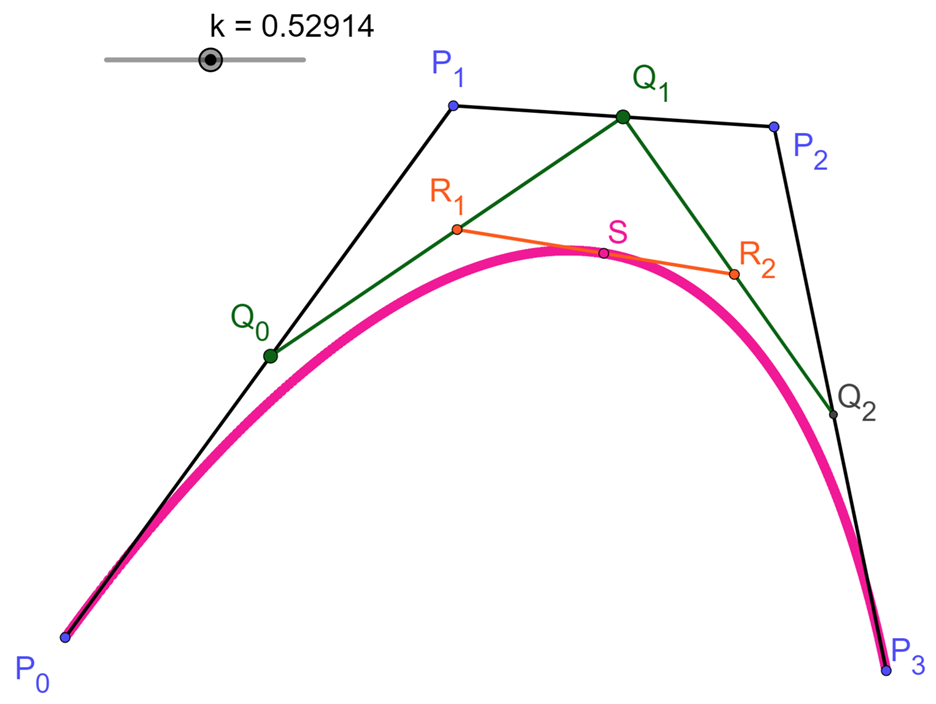
\includegraphics[width= 0.8\linewidth]{11}
		\caption{\small\textit{\color{toanhocdoisong}Hình $7$. Đường cong Bézier bậc $3$ dưới dạng quỹ tích trong GeoGebra.}}
		\vspace*{-10pt}
	\end{figure}
	Với các đường cong Bézier bậc cao hơn, quá trình cũng tương tự, ở mỗi bước ta giảm đi một điểm cho đến khi chi còn lại điểm cuối cùng và tìm quỹ tích của điểm này.
	\vskip 0.1cm
	Cho trường hợp đường cong Bézier bậc $3$, ta có thể thay đổi vị trí các điểm $P_i$ để được các dạng đường cong khác nhau. Có thể thấy, chỉ với tọa độ của vài điểm trong không gian, ta đã có thể xấp xỉ những đường cong phức tạp. Do tính dễ điều chỉnh này mà đường cong Bézier còn được sử dụng để tạo hình động trong đồ họa máy tính. Ta chỉ cần yêu cầu phần mềm thay đổi tọa độ của các điểm điều khiển và toàn bộ đường cong sẽ được di chuyển theo mà không phải đưa ra yêu cầu phức tạp nào khác.
	\begin{figure}[H]
		\vspace*{-5pt}
		\centering
		\captionsetup{labelformat= empty, justification=centering}
		$a)$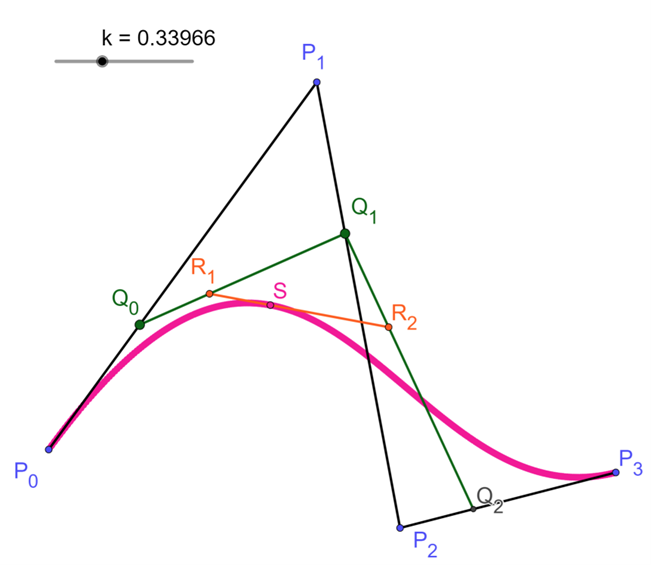
\includegraphics[width= 0.83\linewidth]{12}
		$b)$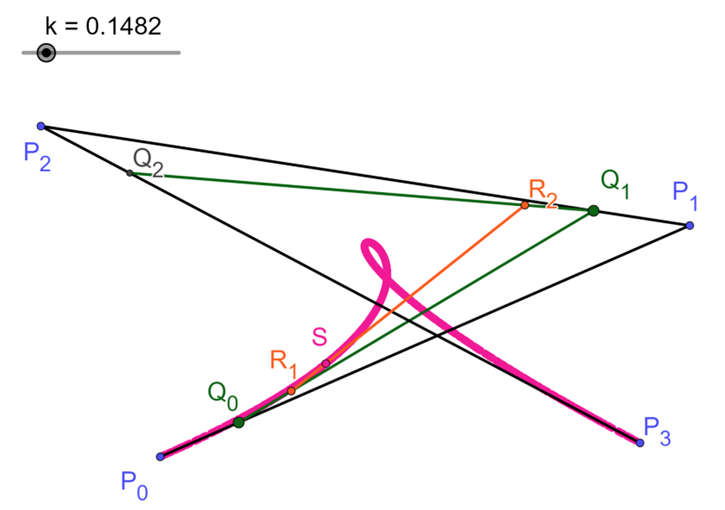
\includegraphics[width= 0.83\linewidth]{13}
		$c)$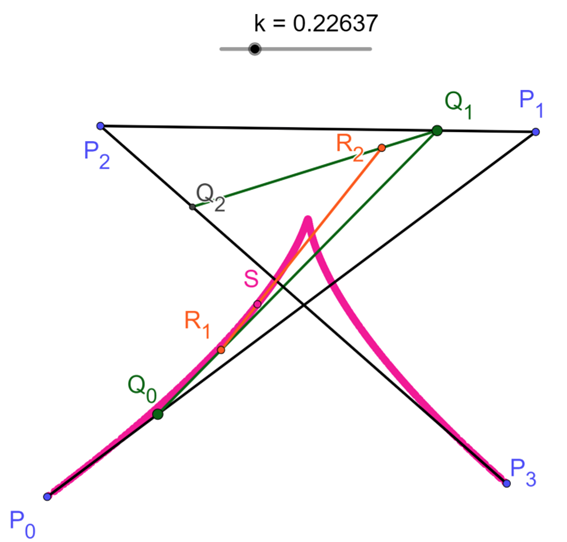
\includegraphics[width= 0.83\linewidth]{14}
		\caption{\small\textit{\color{toanhocdoisong}Hình $8$. Một số dạng đường cong Bézier bậc $3$ khi ta thay đổi vị trí các điểm xác định nó. $a)$ Đường cong có điểm uốn. $b)$ Đường cong có vòng. $c)$ Đường cong có điểm đỉnh.}}
		\vspace*{-5pt}
	\end{figure}
	$\pmb4.$ \textbf{\color{toanhocdoisong}Lời kết}
	\begin{figure}[H]
		\vspace*{-5pt}
		\centering
		\captionsetup{labelformat= empty, justification=centering}
		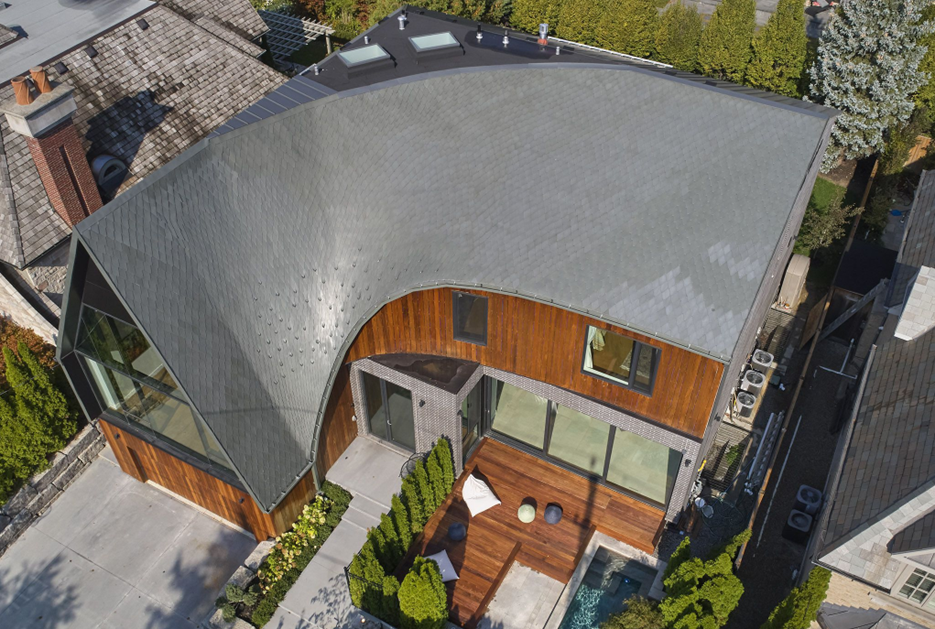
\includegraphics[width= 1\linewidth]{15}
		\caption{\small\textit{\color{toanhocdoisong}Hình $9$. Đường cong Bézier cũng được các kiến trúc sư sử dụng khi thiết kế với sự hỗ trợ của phần mềm. Trong ảnh là một căn nhà có hình dạng mái được thiết kế với đường cong Bézier.}}
		\vspace*{-10pt}
	\end{figure}
	Đường cong Bézier cho thấy ngay cả trong các ngành sản xuất phục vụ đời sống, toán học cũng có thể có những đóng góp quan trọng giúp cải tiến và nâng cao hiệu quả công việc. Toán học được ứng dụng rất phổ biến trong các ngành công nghiệp nhưng vai trò này của nó lại ít được các tài liệu nhắc đến. Việc trình bày về những ứng dụng này cho học sinh sẽ giúp các em có hứng thú hơn với các lĩnh vực khoa học và công nghệ khi định hướng tương lai cho bản thân. Những đường cong hình học còn có nhiều ứng dụng thú vị khác mà Pi sẽ trình bày trong các số sau này với độc giả.
	\begin{figure}[H]
		\vspace*{-5pt}
		\centering
		\captionsetup{labelformat= empty, justification=centering}
		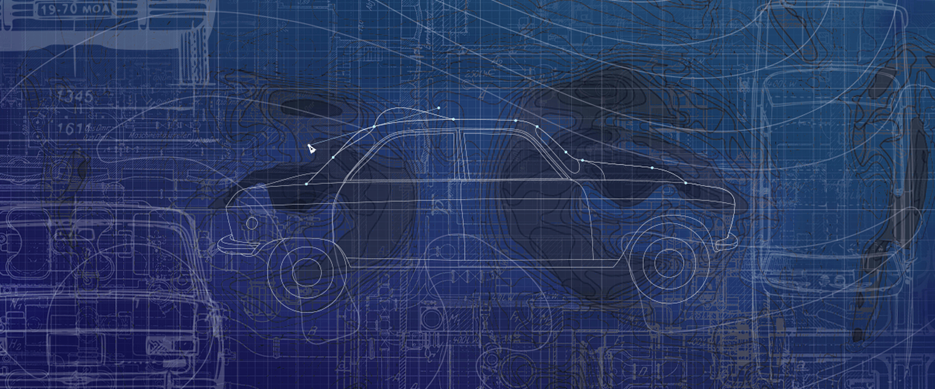
\includegraphics[width= 1\linewidth]{16}
%		\caption{\small\textit{\color{}}}
		\vspace*{-18pt}
	\end{figure}
	\textbf{\color{toanhocdoisong}Phụ lục:} Chứng minh định lý xấp xỉ Weierstrass sử dụng đa thức Bernstein
	\vskip 0.1cm
	Xét 
	\begin{align*}
		B_n(f,t) &= \sum\limits_{i = 0}^n {f\left( {\frac{i}{n}} \right)B_i^n(t)}  \\
		&= \sum\limits_{i = 0}^n {\left( \begin{array}{l}
				n\\
				i
			\end{array} \right){{(1 - t)}^{n - i}}{t^i}f\left( {\frac{i}{n}} \right)}.
	\end{align*}
	Với $t\in [0,1]$, ta có:
	\begin{align*}
		&|f(t) - B_n(f,t) \\
		= &|\left(t + (1-t)\right)^nf(t) - B_n(f,t)|\\
		=&\left| {\sum\limits_{i = 0}^n {B_i^n(t)}  = \left( {f(t) -  - f\left( {\frac{i}{n}} \right)} \right)} \right|\\
		\le &\sum\limits_{i = 0}^n {\left( \begin{array}{l}
				n\\
				i
			\end{array} \right){{(1 - t)}^{n - i}}{t^i}} \left| {f(t) - f\left( {\frac{i}{n}} \right)} \right| = S
	\end{align*}
	\begin{figure}[H]
		\vspace*{-5pt}
		\centering
		\captionsetup{labelformat= empty, justification=centering}
		$a)$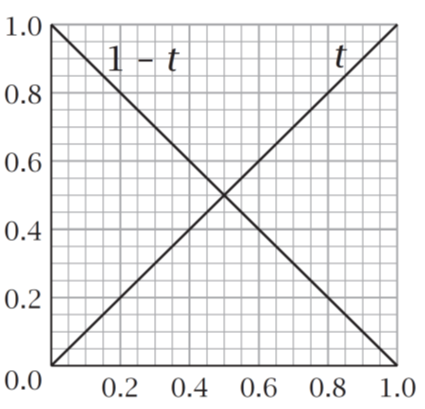
\includegraphics[width= 0.77\linewidth]{17}
		$b)$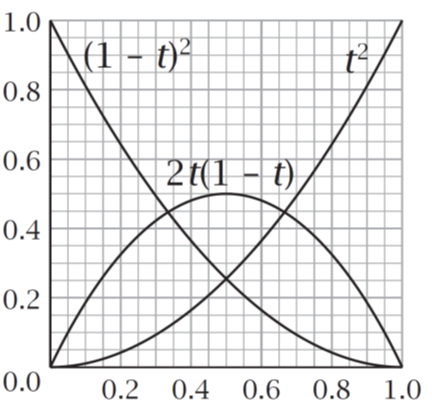
\includegraphics[width= 0.77\linewidth]{18}
		\hspace*{15pt}$c)$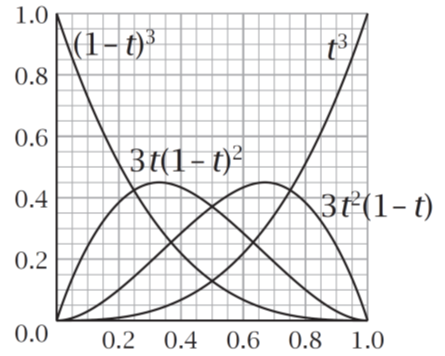
\includegraphics[width= 0.89\linewidth]{19}
		\caption{\small\textit{\color{toanhocdoisong}Hình $9$. $a)$ Các đa thức Bernstein bậc $1$. $b)$ Các đa thức Bernstein bậc $2$. $c)$ Các đa thức Bernstein bậc $3$.}}
		\vspace*{-5pt}
	\end{figure}
	Quan sát đồ thị của các $B_i^n (t)$, ta nhận thấy đỉnh của chúng sẽ gần với một giá trị $t= \dfrac{i}{n}$ và phần lớn diện tích dưới đường cong sẽ phân bố xung quanh đỉnh này. Điều đó có nghĩa rằng các hàm số Bernstein có $\dfrac{i}{n}$ gần với $t$ hơn sẽ có đóng góp nhiều hơn cho $B_n (f,t)$. Do đó, ta có thể tách $S$ thành hai phần như sau với $ \delta >0$:
	\begin{align*}
		S =& \sum\limits_{\left| {\frac{i}{n} - t} \right| \ge \delta }\!\!\! \left(\!\!\!\! \begin{array}{l}
				n\\
				i
			\end{array}\!\!\!\! \right){{(1 \!-\! t)}^{n - i}}{t^i}\left| {f(t) - f\left( {\frac{i}{n}} \right)} \right| \\
		&+ \!\! \sum\limits_{\left| {\frac{i}{n} - t} \right| < \delta }\!\!\! \left(\!\!\!\! \begin{array}{l}
				n\\
				i
			\end{array}\!\!\!\! \right){{(1 \!-\! t)}^{n - i}}{t^i}\left| {f(t) \!-\! f\left(\! {\frac{i}{n}} \!\right)} \right|\\
		=&\,\, S_1 + S_2.
	\end{align*}
	Tiến hành khai triển đại số và sử dụng một số công thức để biến đổi tổ hợp, ta có các công thức sau:
	\begin{align*}
		&\sum\limits_{i = 0}^n {B_i^n(t) = 1}.\\
		&\sum\limits_{i = 0}^n {i \cdot B_i^n(t) = nt.}\\
		&\sum\limits_{i = 0}^n {i(i - 1) \cdot B_i^n(t) = n(n - 1){t^2}.}
	\end{align*}
	Từ ba công thức này ta có:
	\begin{align*}
		&\sum\limits_{i = 0}^n {{{(i - nt)}^2}B_i^n(t)} \\
		=\,\, &\sum\limits_{i = 0}^n \left[ {i(i - 1) - (2nt - 1)i + {n^2}{t^2}} \right]B_i^n \\
		= \,\,&n(n - 1){t^2} - (2nt - 1)nt + {n^2}{t^2} \\
		= \,\,&nt(1 - t) \le \frac{n}{{4.}}
	\end{align*}
	Chia cả hai vế cho $n^2$ ta được:
	\begin{align*}
		\sum\limits_{i = 0}^n {{{\left( {\frac{i}{n} - t} \right)}^2}B_i^n(t) \le \frac{1}{{4n}}.}
	\end{align*}
	Do đó:
	\begin{align*}
		\sum\limits_{\left| {\frac{i}{n} - t} \right| \ge \delta } {B_i^n(t)} &\le  \frac{1}{{{\delta ^2}}}\sum\limits_{\left| {\frac{i}{n} - t} \right| \ge \delta } {{\left( {\frac{i}{n} - t} \right)}^2}B_i^n(t) \\
		&\le \frac{1}{{{\delta ^2}}} \cdot \frac{1}{{4n}}.
	\end{align*}
	Với giá trị $M$ thỏa mãn $|f(t)| \le M$ trên $[0,1]$, ta có:
	\begin{align*}
		{S_1} &\le \sum\limits_{\left| {\frac{i}{n} - t} \right| \ge \delta } \left| {f(t) - f\left( {\frac{i}{n}} \right)} \right|B_i^n(t) \\
			&\le 2M \cdot \frac{1}{{4n{\delta ^2}}} = \frac{M}{{2{\delta ^2}n}}.
	\end{align*}
	Với một giá trị $\epsilon$ cho trước, với $\delta$ đủ nhỏ sao cho $|f(u)-f(v)| \le \dfrac{\epsilon}{2}$ khi $|u-v|< \delta$ trong khoảng $[0,1]$, ta có:
	\begin{align*}
		{S_2} \le \sum\limits_{\left| {\frac{i}{n} - t} \right| \ge \delta } {\frac{\epsilon}{2} \cdot B_i^n(t)}  < \frac{\epsilon}{2}\sum\limits_{i = 0}^n {B_i^n(t) = \frac{\epsilon}{2}}.
	\end{align*}
	Tóm lại, với $\epsilon>0$ cho trước và $\delta$ thỏa mãn điều kiện nêu ở trên, khi $n$ đủ lớn để $\dfrac{M}{2\delta^2n} < \dfrac{\epsilon}{2}$, ta có:
	\begin{align*}
		|f(x)- B_{n,f}(t)| < \dfrac{\epsilon}{2} + \dfrac{\epsilon}{2} = \epsilon.
	\end{align*}
	Thay vì biến đổi sử dụng các công thức tổ hợp, ta cũng có thể sử dụng bất đẳng thức Chebyshev trong xác suất để chứng minh $S_1 \le \dfrac{M}{2\delta^2n}$. Bất đẳng thức Chebyshev được phát biểu như sau: Cho $p$ là một phân phối rời rạc với giá trị trung bình $m$ và độ lệch chuẩn $\sigma$, khi đó: $P(|x-m| \ge s \cdot \sigma) \le \dfrac{1}{s^2}$ (chứng minh của bất đẳng thức này không quá phức tạp và có thể được tìm thấy trong các giáo trình xác suất hoặc qua internet). Với trường hợp của ta, $B_i^n (t)$ là các giá trị ứng với $p(x=i)$ của phân phối nhị thức có trung bình là $m=nt$. Độ lệch chuẩn tương ứng của phân phối này sẽ là $\sigma = \sqrt{nt(1-t)}$. Theo bất đẳng thức Chebyshev, chọn $s$ sao cho $s \cdot \dfrac{\sigma}{n} = \delta$, ta có:
	\begin{align*}
		&P\left(|x- nt| \ge s \cdot \sigma\right)\\
		= \,\,&\sum\limits_{\left| {\frac{i}{n} - t} \right| \ge \delta } {B_i^n(t)}  \le \frac{1}{{{s^2}}} \\
		= \,\,&\frac{{{\sigma ^2}}}{{{n^2}{\delta ^2}}} = \frac{{t(1 - t)}}{{n{\delta ^2}}} \le \frac{1}{{4n{\delta ^2}}}.
	\end{align*}
	\textbf{\color{toanhocdoisong}Tài liệu tham khảo}
	\vskip 0.1cm
	[$1$] Farin, Gerald. \textit{Curves and Surfaces for Computer--Aided Geometric Design}. Elsevier, $28$ June $2014$.
	\vskip 0.1cm
	[$2$] Farin, Gerald E, et al. \textit{Handbook of Computer Aided Geometric Design}. Amsterdam ; Boston, Mass., Elsevier, $2002$.
	\vskip 0.1cm
	[$3$] Havil, Julian. \textit{Curves for the Mathematically Curious : An Anthology of the Unpredictable, Historical, Beautiful and Romantic}. Princeton, New Jersey ; Oxford, Princeton University Press, $2019$.
	\vskip 0.1cm
	[$4$] Levasseur, Kenneth M. ``A Probabilistic Proof of the Weierstrass Approximation Theorem.'' T\textit{he American Mathematical Monthly}, vol. $91$, no. $4$, Apr. $1984$, p. $249$, \url{https://doi.org/10.2307/2322960}. Accessed $31$ Oct. $2019$.
	\vskip 0.1cm
	[$5$] Salomon, David. \textit{Curves and Surfaces for Computer Graphics}. New York, Ny, Springer New York, $2006$.
\end{multicols}
%	\newpage
%
%	\setcounter{figure}{0}
%	\thispagestyle{duongvaotoanhocnone}
\pagestyle{duongvaotoanhoc}
\everymath{\color{duongvaotoanhoc}}
\graphicspath{{../duongvaotoanhoc/pic2/}}
\blfootnote{$^*$\color{duongvaotoanhoc}Nguồn: https://www.quantamagazine.org/hobbyist-finds-maths-elusive-einstein-tile-20230404.}
\blfootnote{\color{duongvaotoanhoc}$^1$THPT chuyên Hà Nội -- Amsterdam.}
\begingroup
\AddToShipoutPicture*{\put(0,616){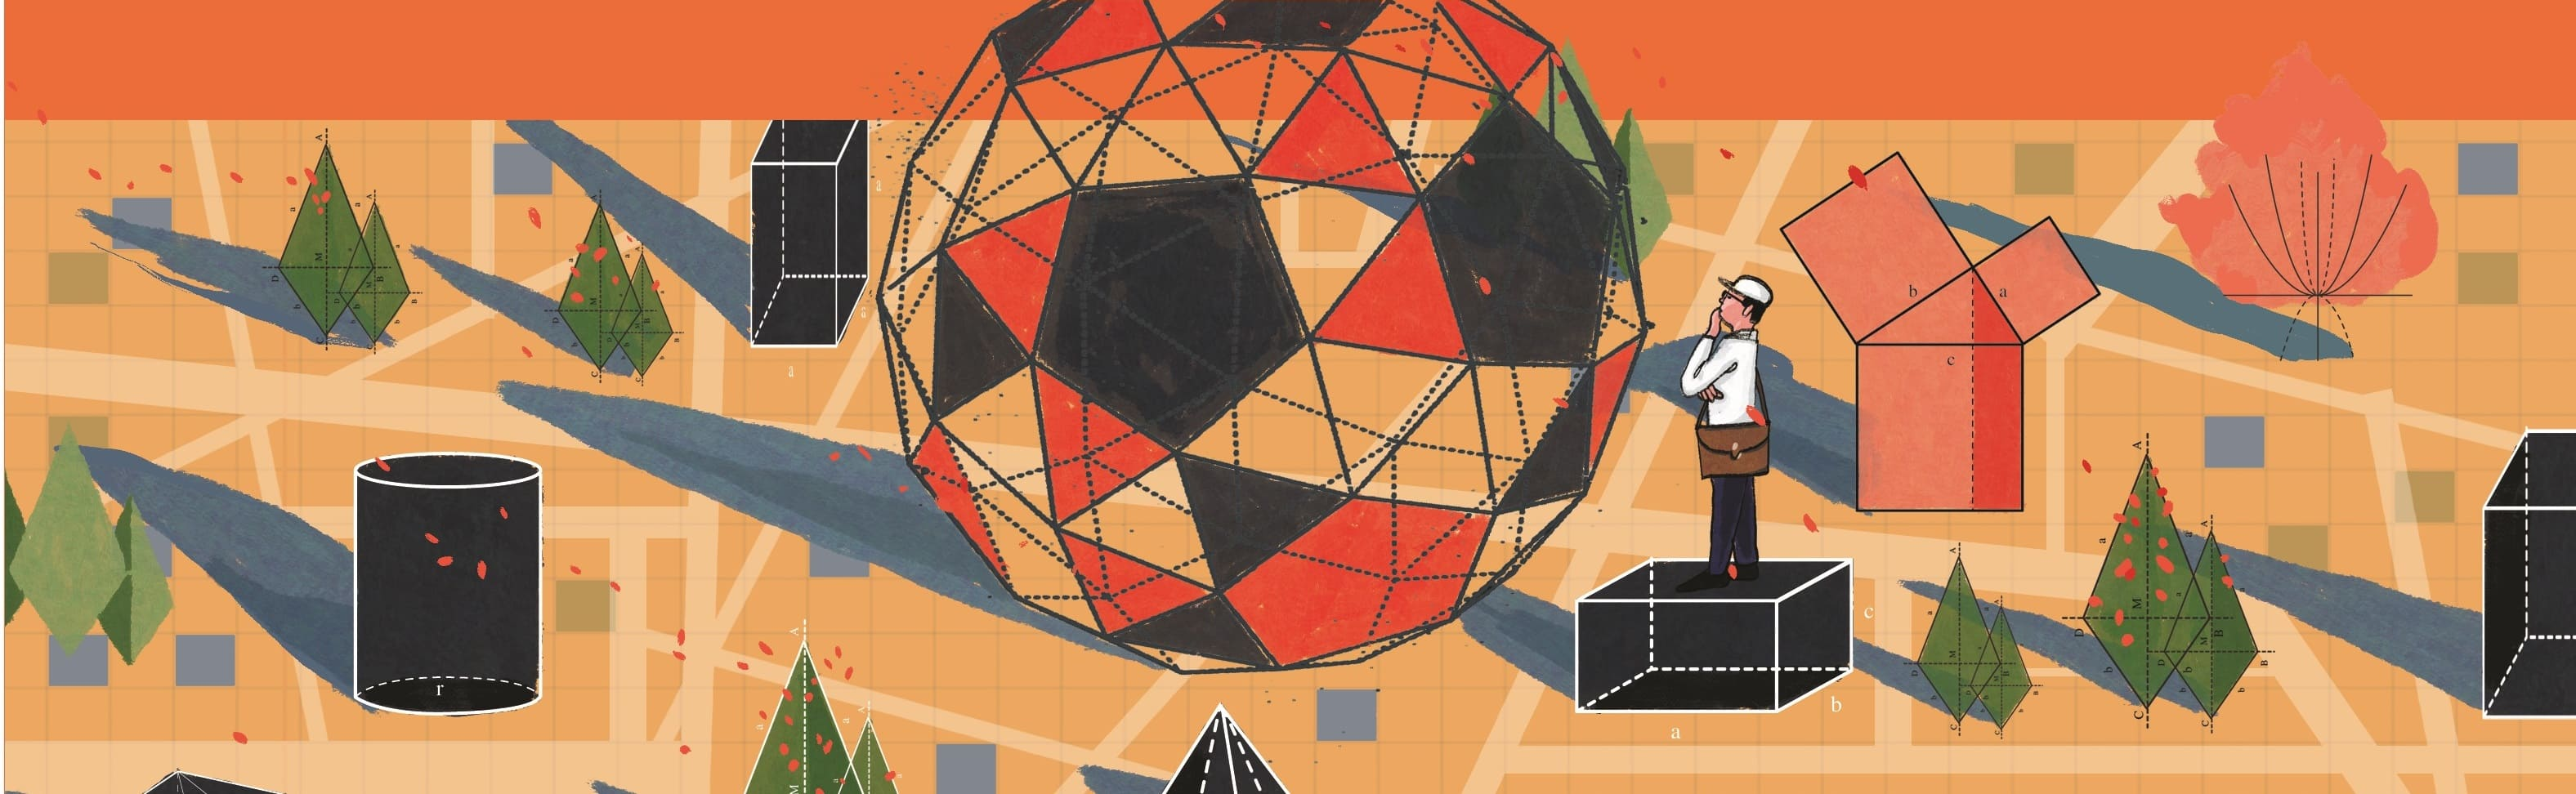
\includegraphics[width=19.3cm]{../bannerduongvao}}}
\AddToShipoutPicture*{\put(76,500){
\includegraphics[scale=1]{../tieude1.pdf}}}
\centering
\endgroup
\vspace*{208pt}

\begin{multicols}{2}	
	Giữa tháng $11$ năm $2022$, David Smith [$1$], một kỹ thuật viên in ấn đã nghỉ hưu có niềm vui thú với xếp hình, hình học fractal và bản đồ đường xá, đang làm việc mình yêu thích: chơi với những hình khối. Nhờ một phần mềm gọi là ``PolyForm Puzzle Solver" [$2$], ông đã dựng được một miếng gạch hình cái mũ trông khá khiêm tốn. Ông đã bắt đầu thử nghiệm xem có thể phủ kín được bao nhiêu phần màn hình với duy nhất viên gạch lát này, với điều kiện không để hai viên đè lên nhau hay để hở khoảng trống.
	\vskip 0.1cm
	Thường thì khi ông tạo ra loại gạch mới, chúng sẽ hoặc tạo thành một họa tiết lặp, hoặc chỉ lát được một phần nhỏ màn hình. Viên gạch mũ có vẻ không thuộc cả hai loại này. Thế là Smith cắt $30$ miếng giấy bìa màu hình viên gạch này và xếp chúng trên bàn. Rồi ông cắt thêm $30$ cái nữa và tiếp tục xếp. ``Tôi dần nhận ra rằng mỗi lần xếp là một cách lát tôi chưa thấy bao giờ," ông nói. ``Đó là một viên gạch lát ranh mãnh". Ông gửi mô tả về viên gạch tới Craig Kaplan [$3$], một nhà khoa học máy tính ông quen tại Đại học Waterloo, Canada. Kaplan ngay lập tức bắt đầu tìm hiểu các tính chất của nó.
	\vskip 0.1cm
	Ngày $20$ tháng $3$ vừa qua, Smith và Kaplan, cùng với $2$ nhà nghiên cứu nữa, đã công bố [$4$] rằng đây chính là thứ mà các nhà toán học đã tìm kiếm suốt hơn năm thập kỉ: một viên gạch duy nhất mà ta có thể dùng để lát toàn mặt phẳng, nhưng chỉ theo những họa tiết không lặp lại bất kỳ khối gạch nào. Các nhà toán học gọi những viên gạch, hoặc các bộ viên gạch, có tính chất đó là ``phi tuần hoàn" (aperiodic), trái với hình vuông hoặc lục giác là những hình có thể phủ cả mặt phẳng theo các họa tiết lặp lại (hay ``tuần hoàn").
	\vskip 0.1cm
	Viên gạch mũ ẩn chứa ``đủ sự phức tạp để bẻ gãy trật tự tuần hoàn theo mọi quy mô", các nhà nghiên cứu khẳng định trong bài báo. Hơn nữa, họ nhận ra rằng viên gạch mũ là một trong vô số viên gạch khác nhau có cùng tính chất này.
	\vskip 0.1cm
	``Tưởng xa tận chân trời mà gần ngay trước mắt,"  là những gì  Doris Schattschneider, giáo sư toán danh dự tại Đại học Moravian, Pennsylvania nói về viên gạch này.  Bà tả rằng bản thân đã ``sửng sốt" trước phát hiện này.
	\vskip 0.1cm
	Các nhà toán học đã bắt đầu tìm kiếm một viên gạch như viên gạch mũ từ những năm 60 thế kỷ trước, khi Robert Berger  [$5$] dựng ra $20426$ loại gạch cùng nhau lát mặt phẳng một cách phi tuần hoàn. Công trình này là phát súng mở màn cho một cuộc đua dựng ra các bộ gạch có thể lát mặt phẳng phi tuần hoàn bằng ít loại hơn, lên đến đỉnh điểm là khám phá của Roger Penrose vào thập niên $70$ với chỉ hai viên. Năm $1982$, Dan Shechtman [$6$] đã tìm ra những dạng đối xứng tương tự như của gạch lát Penrose trong tự nhiên, dưới hình hài các cấu trúc gọi là giả tinh thể (quasicrystal), qua đó giúp ông đạt giải Nobel Hóa học năm $2011$.
	\begin{figure}[H]
		\vspace*{-5pt}
		\centering
		\captionsetup{labelformat= empty, justification=centering}
		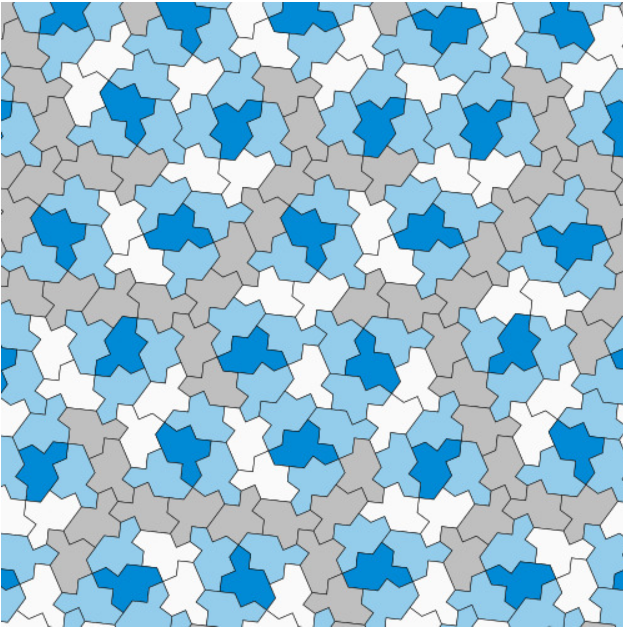
\includegraphics[width= 1\linewidth]{1}
		\caption{\small\textit{\color{duongvaotoanhoc}Viên gạch mũ chỉ là một trong một họ các viên gạch phi tuần hoàn}}
		\vspace*{-10pt}
	\end{figure}
	Từ ấy, các nhà toán học vẫn không ngừng tìm kiếm một loại gạch duy nhất có thể lát mặt phẳng $2$ chiều một cách phi tuần hoàn, mà không cho phép kẽ hở hay gạch đè lên nhau. Ludwig Danzer, một nhà hình học người Đức, đã tinh nghịch đặt tên cho loại gạch như thế là một ``einstein" -- chơi chữ của cụm từ tiếng Đức ``ein stein", nghĩa là ``một miếng".
	\vskip 0.1cm
	Vào những năm $1990$, hai nhóm khác nhau  [$7$] đã tìm ra cách chồng kề nhau một loại gạch $10$ cạnh để phủ mặt phẳng. Trong thập kỷ sau đó, Joan Taylor [$8$], một nhà toán học nghiệp dư ở Tasmania, đã khám phá ra một hình với nhiều miếng không liền  với nhau  [$9$]. Cùng với Joshua Socolar [$10$], một nhà vật lý tại Đại học Duke, họ đã chứng minh được hình này có thể lát mặt phẳng một cách phi tuần hoàn  [$11$]. Và mới năm ngoái, Rachel Greenfield [$12$] từ Viện Nghiên cứu Cao cấp Princeton và Terence Tao [$13$] từ Đại học California, Los Angeles đã phát hiện ra một hình trong không gian nhiều chiều [$14$] có thể lát không gian một cách phi tuần hoàn mà không cần quay hay lật.
	\vskip 0.1cm
	Nhưng chưa ai tìm được một ``einstein" đích thực -- một hình $2$ chiều đơn giản phủ mặt phẳng một cách phi tuần hoàn. Cuối cùng, giới toán học bắt đầu nghi ngờ sự tồn tại của chúng, theo lời Marjorie Senechal [$15$], một nhà nghiên cứu về lát gạch và giáo sư danh dự tại Đại học Smith. Bà cho biết thêm: việc một ``einstein" đơn giản như viên gạch mũ của Smith lù lù trước mắt, chờ đợi được tìm ra là một sự thật ``khó tin". 
	\vskip 0.1cm
	Theo bà phỏng đoán, có lẽ lý do viên gạch mũ tránh được sự tìm kiếm đến tận bây giờ là do nhiều nhà toán học đã tập trung vào các hình đối xứng kiểu ``cấm kỵ" -- những kiểu mà không thể có trong các loại gạch lát tuần hoàn. Chẳng hạn như gạch lát Penrose có ``đối xứng gấp $5$" (đối xứng qua phép quay $72$ độ quanh tâm), như ở các ngũ giác đều hay hình ngôi sao. Các ngũ giác đều không thể phủ mặt phẳng, nên bắt đầu từ các ``đối xứng gấp $5$" là khởi điểm khá tự nhiên. 
	\vskip 0.1cm
	Trái lại, viên gạch mũ chẳng có đối xứng nào cả, và ``đơn giản đến mức tầm thường", các tác giả bình luận. Cách lát này có quan hệ mật thiết với một cách lát tuần hoàn: lưới tổ ong hình lục giác. Ta có thể tạo ra cách lát hình mũ từ cách lát bằng lục giác như sau: trước hết nối các trung điểm các cặp cạnh đối của lục giác. Lục giác sẽ bị chia thành 6 hình ``cánh diều". Mỗi viên gạch mũ được cấu thành từ $8$ hình cánh diều liền nhau, kết hợp từ các lục giác kề nhau. Bất kỳ ai đầu tư chút sức lực, cùng một cái bút dạ và sàn nhà vệ sinh gạch hình lục giác cũng có thể viền được một cách phủ mặt phẳng bằng hình mũ.  
	\begin{figure}[H]
		\vspace*{-5pt}
		\centering
		\captionsetup{labelformat= empty, justification=centering}
		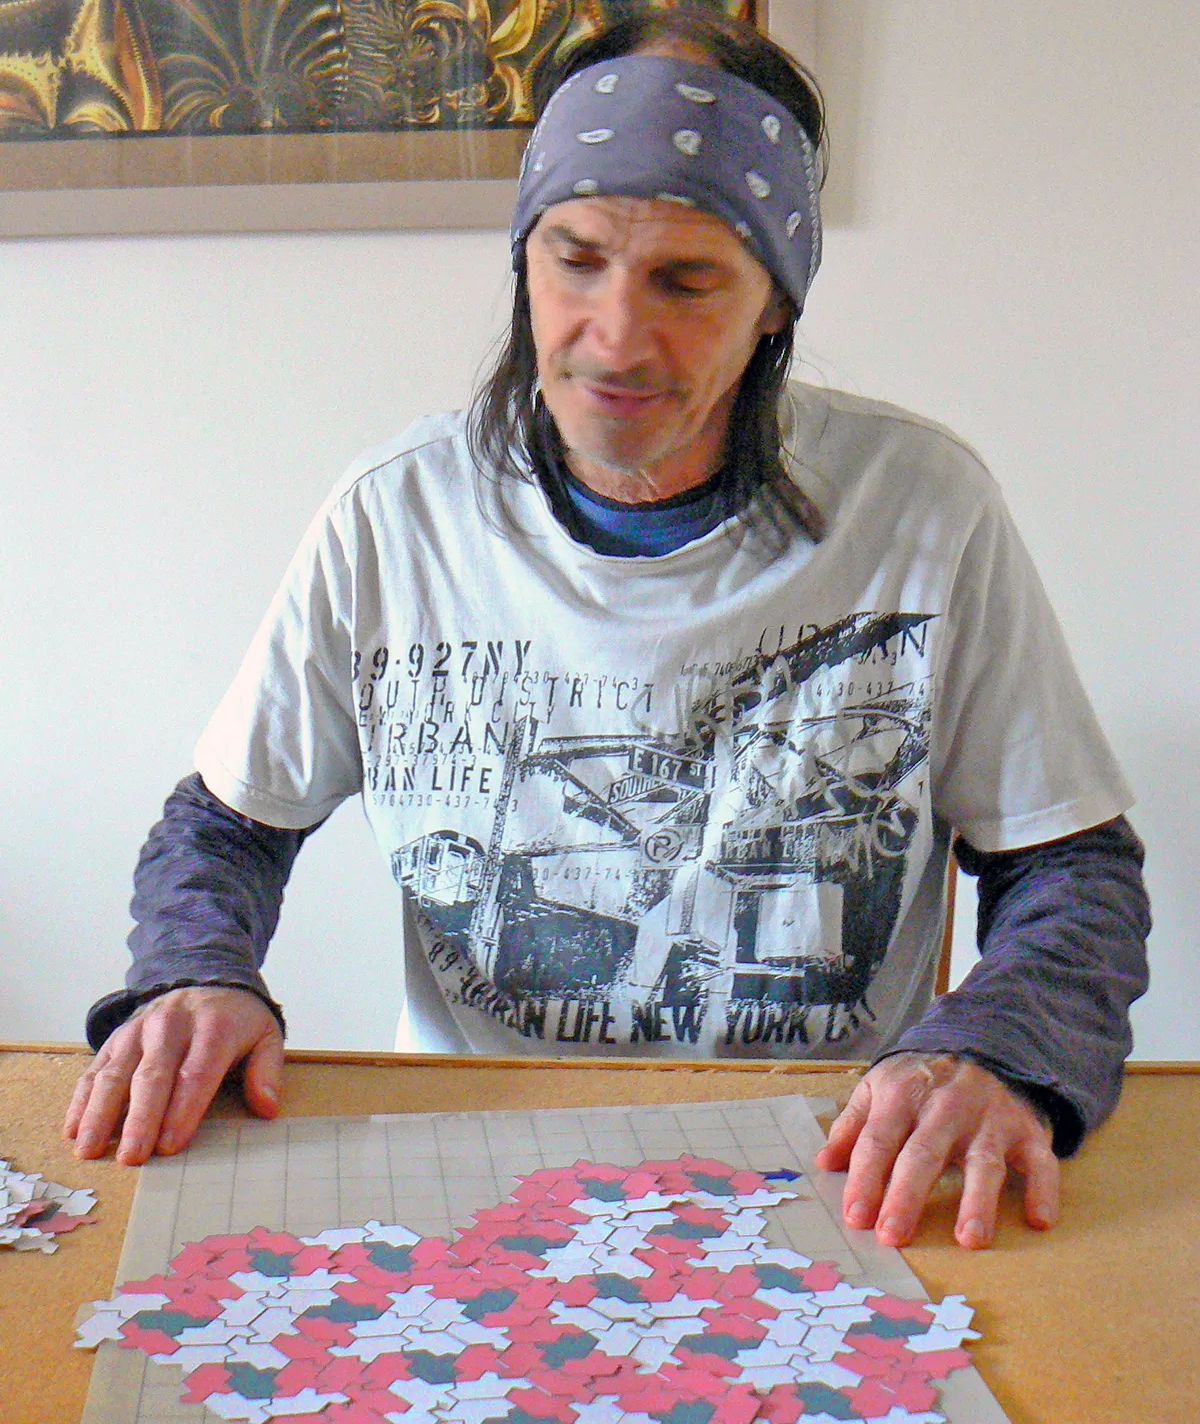
\includegraphics[width= 1\linewidth]{2}
		\caption{\small\textit{\color{duongvaotoanhoc}Khám phá của David Smith được coi là một khám phá khó tin.}}
		\vspace*{-10pt}
	\end{figure}
	Viên gạch mũ, Senechal nói, chỉ ra rằng sự liên kết giữa gạch lát tuần hoàn và phi tuần hoàn chặt chẽ hơn ta tưởng.
	\vskip 0.1cm
	Kể từ lúc thông báo phát hiện này, các nhà toán học và người yêu thích lát gạch đã đổ xô tìm tới những loại gạch mới này, cắt chúng ra từ giấy, in $3$--D, và làm trang trí họa tiết cho mũ và bánh quy của họ. Phong trào ấy đem lại một cảm giác ``hơi siêu thực" cho Smith, một cư dân tại thành phố ven biển Bridlington phía bắc nước Anh. ``Tôi không quen với mấy việc kiểu như thế này".
	\vskip 0.1cm
	Nhưng đây không phải là lần đầu tiên một cá nhân nghiệp dư với niềm đam mê to lớn tạo đột phá trong lát gạch. Robert Ammann, một nhân viên phân loại thư, đã độc lập tìm ra một trong các bộ gạch lát Penrose [$16$] vào những năm $70$. Marjorie Rice, một bà nội trợ ở California, tìm ra cả một họ gạch lát hình ngũ giác [$17$] vào năm $1975$. Và ta có Joan Taylor cùng gạch lát Socolar -- Taylor. Có lẽ những người như họ, khác với các nhà toán học, ``không biết về độ khó của bài toán, vì thế không bị áp lực tâm lý", Senechal nói.
	\vskip 0.1cm
	Với các viên gạch có thể lát mặt phẳng một cách tuần hoàn, thì dùng chúng để lát mặt phẳng một cách không tuần hoàn là tương đối đơn giản. Ví dụ như đặt ngang một vài quân domino trong khi các quân domino khác để dọc. ``Nghệ thuật thực sự là tìm một viên gạch với khả năng lát mặt phẳng, nhưng không thể làm vậy một cách tuần hoàn." Socolar nói.
	\vskip 0.1cm
	Ta không thể tạo ra một thuật toán xác định được liệu một tập hợp các viên gạch nào đó có thể lát mặt phẳng hay không (dù theo cách tuần hoàn hay phi tuần hoàn đi chăng nữa). Nên sau khi được Smith giới thiệu viên gạch mũ, Kaplan đã sử dụng một chương trình ông viết có khả năng đặt các viên gạch bao quanh một viên gốc và mở rộng dần dần từ đó. Ngoài các viên gạch lát mặt phẳng tuần hoàn, chưa ai từng tìm được loại gạch lát nào mà có thể lát quá $6$ vòng quanh viên gạch gốc. Lần này, chương trình cứ chạy và chạy mãi, và nó lát tới tận $16$ vòng gạch mũ trước khi Kaplan dừng chương trình vì đã thu thập đủ dữ liệu.
	\vskip 0.1cm
	Trong khi đó, trước sự kinh ngạc của Kaplan, Smith có một khám phá mới: một viên gạch thứ hai, hình dạng giống một con rùa, cũng thuộc loại phi tuần hoàn. ``Chỉ ra được $2$ einstein liên tiếp thật là ngoài sức tưởng tượng," nhóm nghiên cứu viết.
	\vskip 0.1cm
	Giữa tháng $1$, Smith và Kaplan đã tuyển dụng được $2$ nhà nghiên cứu nữa: Chaim Goodmain--Strauss [$18$], một nhà toán học ở Bảo tàng Toán học Quốc gia và Đại học Arkansas, và Joseph Samuel Myers [$19$], một kỹ sư phần mềm ở Cambridge, Anh, với bằng tiến sỹ tổ hợp. Myers dốc toàn bộ thời gian rảnh của mình cho viên gạch mũ, và chỉ trong hơn một tuần, ông đã chứng minh được nó phi tuần hoàn. ``Chúng tôi khá sốc bởi tốc độ ông ấy giải bài toán này," Kaplan nói.
	\begin{figure}[H]
		\vspace*{5pt}
		\centering
		\captionsetup{labelformat= empty, justification=centering}
		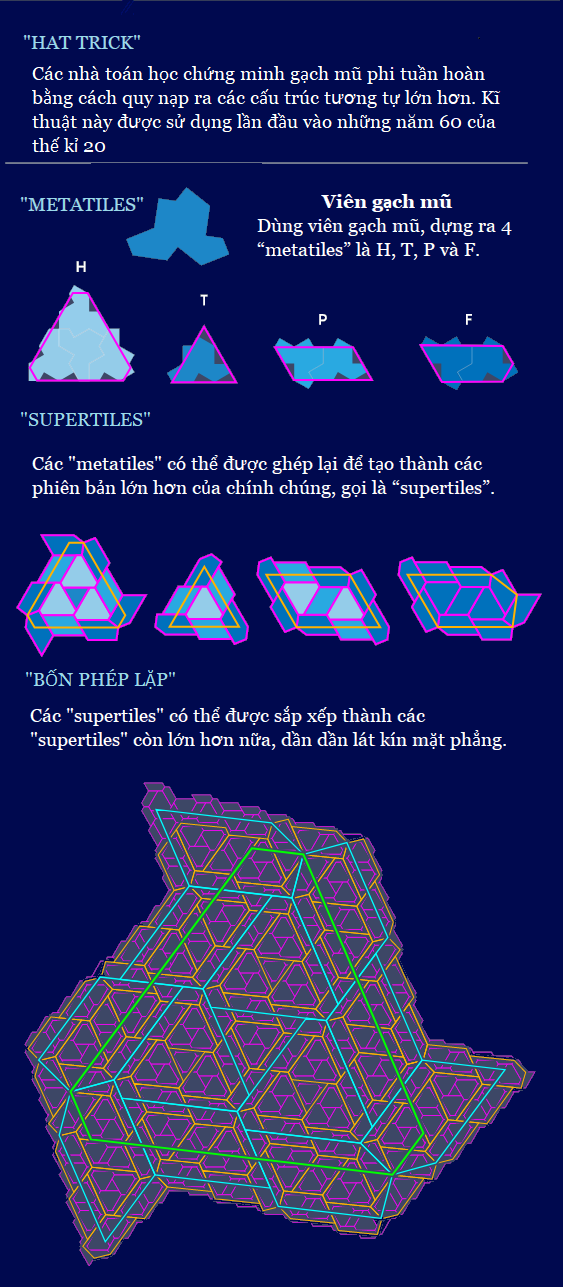
\includegraphics[width= 1\linewidth]{3}
		%		\caption{\small\textit{\color{}}}
		\vspace*{-20pt}
	\end{figure}
	Chứng minh này được biến tấu từ một phương pháp của Berger vào những năm $1960$. Phương pháp đó bao gồm việc ghép một số viên gạch lại với nhau, tạo thành những phiên bản lớn hơn của chính chúng, hình thành một cấu trúc phân chia đẳng cấp. Đầu tiên, Myers xác định bốn hình trung gian được tạo từ viên gạch mũ, gọi là $H$, $T$, $P$ và $F$. Ví dụ, viên gạch $H$ được tạo ra từ $4$ viên gạch mũ, ghép lại thành một hình hao hao một tam giác cụt ở các góc. Myers chứng minh rằng có thể ghép $4$ hình lại với nhau để tạo ra vẫn $4$ hình đó với kích thước lớn hơn. Chẳng hạn, có thể tạo ra một viên gạch $H$ lớn bằng cách xếp ba viên gạch $H$ quanh một viên gạch $T$, rồi ghép các viên gạch $P$ và $F$ xung quanh hình vừa tạo.
	\vskip 0.1cm
	Phương pháp này giúp ta dựng ra những viên gạch lớn dần. Có thể bắt đầu với bất kỳ loại gạch nào, chẳng hạn như viên gạch $H$, phóng to nó lên, và lấp đầy các khe hở  bằng $4$ hình trung gian $H$, $T$, $P$, $F$. Ta có thể lặp đi lặp lại việc này vô số lần để tạo ra một cấu trúc phân cấp từ những hình này, từ đó lát kín mặt phẳng. Đơn vị cơ bản của cấu trúc chính là những viên gạch mũ. 
	\vskip 0.1cm
	Họ đã chứng minh được cách lát hình thành từ các cấu trúc phân cấp này không bao giờ tuần hoàn. Đồng thời họ cũng chỉ ra rằng đó là cách duy nhất để phủ mặt phẳng bằng các hình mũ. Vì thế nên cách phủ mặt phẳng bằng các viên gạch mũ không thể tuần hoàn. ``Một kết quả rất tuyệt vời", Socolar cho hay.
	\vskip 0.1cm
	Vậy là còn lại loại gạch lát thứ hai Smith phát hiện: con rùa. Liệu chăng việc một người đàn ông khám phá ra tận hai loại lát gạch phi tuần hoàn cùng lúc, trong khi phần còn lại của nhân loại bó tay trong suốt 50 năm, đơn thuần là một sự trùng hợp tuyệt diệu? Viên gạch mũ và ``con rùa" nhìn giống nhau đến bất ngờ, khiến các nhà nghiên cứu nghi ngờ rằng con rùa cũng là một viên gạch phi tuần hoàn. Nhưng nghi ngờ vẫn chỉ là nghi ngờ, không phải chứng minh.
	\vskip 0.1cm
	Thế rồi Myers có một khám phá: hóa ra, cả cái mũ và con rùa đều thuộc về một họ gồm vô số viên gạch lát mặt phẳng theo cùng một cách.
	\vskip 0.1cm
	Mỗi viên gạch mũ có $13$ cạnh: $6$ dài, $6$ ngắn tương ứng với các cạnh hình cánh diều, cộng với một cạnh ghép từ hai cạnh cánh diều ngắn. Bằng cách thay đổi kích cỡ độ dài các cạnh của viên gạch mũ, ta có thể thu được vô hạn không đếm được các viên gạch phi tuần hoàn. Tưởng tượng một thanh trượt: di sang trái khiến cạnh ngắn (cùng với một cạnh ghép kể trên) ngắn đi; di sang phải thì cạnh dài nhỏ lại. ``Con rùa" nằm về bên phải so với viên gạch mũ, nhưng đồng thời cũng có vô số hình khác thuộc kiểu tương tự.
	\vskip 0.1cm
	Nếu ta đẩy thanh trượt hết nấc về bên trái, cạnh ngắn sẽ biến mất, viên gạch lúc này có hình chữ $V$ $6$ cạnh;  đẩy hết nấc sang phải thì cạnh dài biến mất và ta được một hình bảy cạnh được đặt tên là ``sao chổi".  Khác với viên gạch mũ, gạch hình chữ $V$ và hình sao chổi có thể được dùng để lát mặt phẳng một cách tuần hoàn. Hình ở trung tâm thanh trượt, tức cạnh dài và cạnh ngắn bằng nhau, cũng có tính chất này.
	\begin{figure}[H]
		\vspace*{-5pt}
		\centering
		\captionsetup{labelformat= empty, justification=centering}
		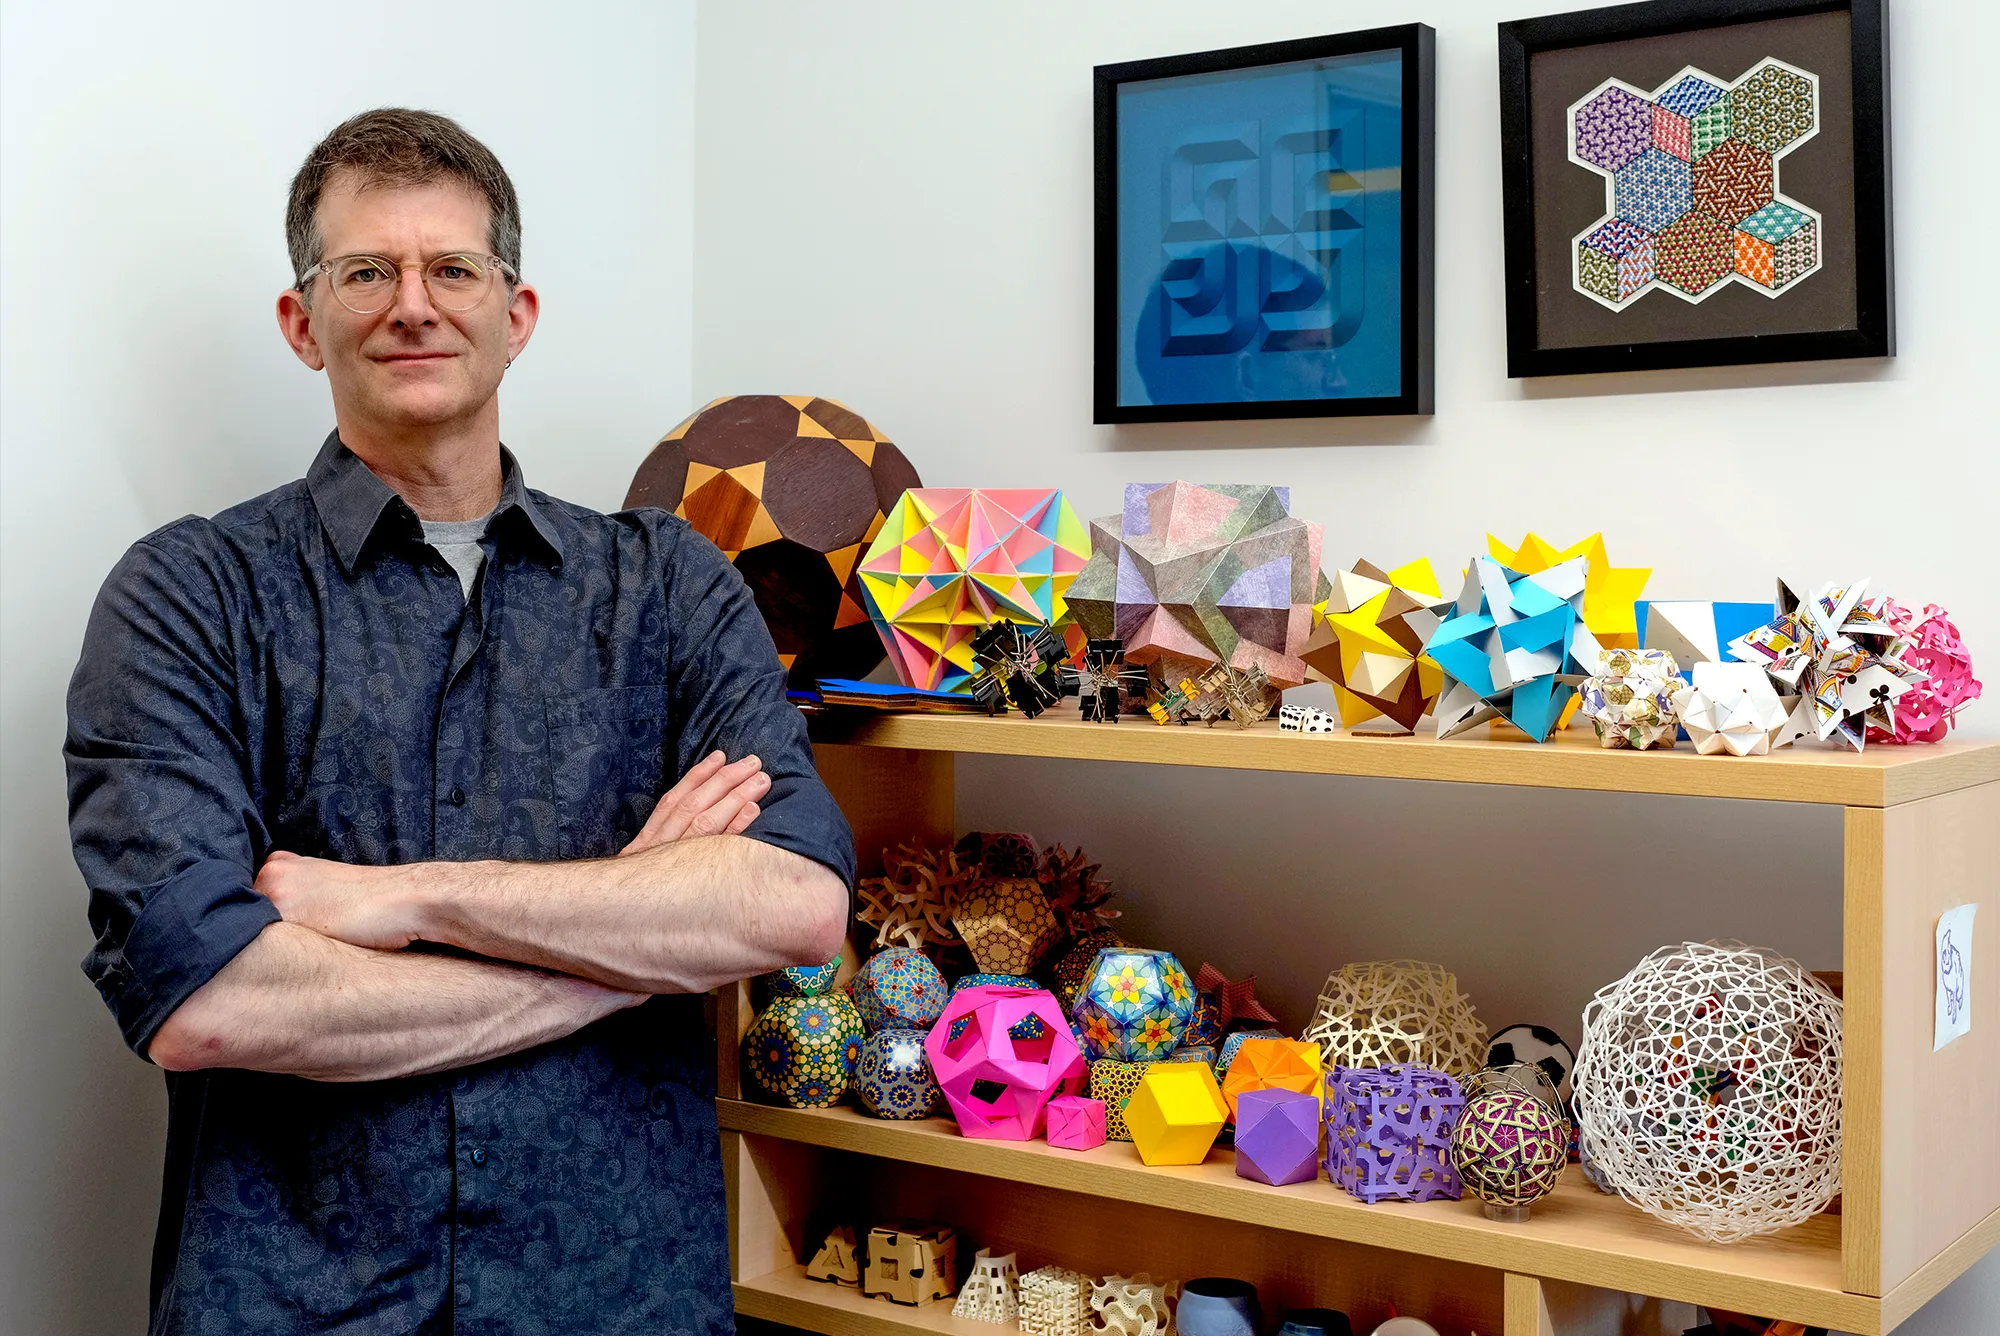
\includegraphics[width= 1\linewidth]{6}
		\caption{\small\textit{\color{duongvaotoanhoc}Craig Kaplan, nhà khoa học máy tính ở đại học Waterloo, Canada.}}
		\vspace*{-10pt}
	\end{figure}
	Myers còn nhận ra rằng mình có thể sử dụng đặc tính hình học của viên gạch chữ $V$ và sao chổi để chứng minh là tất cả các hình dọc theo thanh trượt, trừ hai đầu và trung điểm, đều là gạch loại phi tuần hoàn. Lập luận này, được Kaplan gọi là ``một nước đi thiên tài của Toán học", hoàn toàn mới lạ với bộ môn lát gạch. Trước đây, lĩnh vực này chỉ có $3$ cách tiếp cận chính để chứng minh tính phi tuần hoàn, theo lời Goodman-Strauss. ``Giờ ta có cách thứ tư." 
	\vskip 0.1cm
	Các nhà toán học đang cố gắng thấm phương pháp chứng minh mới này. ``Tôi phải ngồi lại và nghiêm túc dành thời gian cho thứ này," Senechal nói. 
	\vskip 0.1cm
	Một câu hỏi tự nhiên, Greenfield nói, là liệu rằng có thể tìm được một nguồn nào đó tạo ra các cách lát mới không. Năm $1981$, Nicholaas de Brujin [$20$] đã chứng minh được các cách lát Penrose là hình chiếu xuống không gian $2$ chiều của các viên gạch lát tuần hoàn mặt phẳng $5$ chiều. ``Nếu tương tác hoặc cấu trúc của những cách lát (mới) này tương ứng với một cách lát gạch tuần hoàn trên không gian nhiều chiều hơn, điều ấy sẽ thực sự thú vị để tìm hiểu." Greenfield nói.
	\vskip 0.1cm
	Với tư cách một nhà vật lý, Socolar đã bắt đầu khám phá tính chất vật liệu của cách lát mới này. Ông thấy rằng: kiểu nhiễu xạ khi ánh sáng chiếu qua loại gạch lát này có những đỉnh dốc tương tự như ở giả tinh thế. Kể cả khi ấy, cách lát bằng gạch hình mũ vẫn ``trông khác hẳn với tất cả những thứ tôi từng thấy trước đây", ông khẳng định.
	\vskip 0.1cm
	Trong lúc ấy, Smith chưa xong việc với viên gạch ranh mãnh của ông. Ông hiện dự định khám phá tiềm năng nghệ thuật và cách phối màu để làm nổi bật họa tiết của các viên gạch này. ``Dường như nó có thái độ riêng," ông nói. ``Tôi nghĩ ta nên tôn trọng khi làm việc với nó."
	\vskip 0.1cm
	Bình luận của các dịch giả: Có ý kiến cho rằng cái mũ chưa thể được tính là ``einstein" do thực chất chúng ta cần dùng tới cả cái mũ và viên gạch đối xứng trục với nó để lát toàn mặt phẳng, và hai viên gạch có thể tính là khác nhau. Tuy nhiên, đúng như lời hứa, David Smith đã có một phát hiện mới: một trong các họ hàng đặc biệt của cái mũ, gọi là Tile($1, 1$), có thể lát mặt phẳng một cách phi tuần hoàn nếu như ta cấm úp ngược viên gạch lại để ghép. Bằng cách điều chỉnh các cạnh của Tile($1, 1$), ông thu được một họ các viên gạch gọi là bóng ma. Lần này, mỗi bóng ma đều tự nó lát được mặt phẳng phi tuần hoàn, kể cả khi cho phép úp ngược viên gạch này để ghép. Bài báo về phát hiện này [$21$] được đăng lên arXiv vào cuối tháng $5$ năm $2023$, tại thời điểm đăng bài hiện chúng tôi chưa rõ tính xác thực.
	\vskip 0.1cm
	\textbf{\color{duongvaotoanhoc}Các liên kết trong bài viết}
	\vskip 0.1cm 
	[$1$] https://the-orangery.weebly.com/
	\vskip 0.1cm
	[$2$] https://www.jaapsch.net/puzzles/polysol\\
	ver.htm
	\vskip 0.1cm
	[$3$] https://cs.uwaterloo.ca/~csk/
	\vskip 0.1cm
	[$4$] https://arxiv.org/abs/2303.10798
	\vskip 0.1cm
	[$5$] https://www.ams.org/books/memo/00\\
	66/
	\vskip 0.1cm
	[$6$] https://www.engineering.iastate.edu/peo\\
	ple/profile/dannys/
	\vskip 0.1cm
	[$7$] https://link.springer.com/article/10.1007/\\
	BF00239998
	\vskip 0.1cm
	[$8$] http://taylortiling.com/
	\vskip 0.1cm
	[$9$] https://sfb701.math.uni-bielefeld.de/prep\\
	rints/sfb10015.pdf
	\vskip 0.1cm
	[$10$] https://scholars.duke.edu/person/socolar
	\vskip 0.1cm
	[$11$] https://arxiv.org/abs/1003.4279v2
	\vskip 0.1cm
	[$12$] https://www.math.ias.edu/~rgreenfeld/
	\vskip 0.1cm
	[$13$] https://www.math.ucla.edu/~tao/
	\vskip 0.1cm
	[$14$]https://www.quantamagazine.org/nasty-geometry-breaks-decades-old-tiling-conjectur\\
	e-20221215/
	\vskip 0.1cm
	[$15$] http://www.science.smith.edu/~senechal/
	\vskip 0.1cm
	[$16$] https://link.springer.com/article/10.1007\\
	/BF02985414
	\vskip 0.1cm
	[$17$] https://www.quantamagazine.org/marjo\\
	rie-rices-secret-pentagons-20170711/
	\vskip 0.1cm
	[$18$]https://fulbright.uark.edu/departments/\\
	math/directory/index/uid/strauss/name/Chai\\m+Goodman-strauss/
	\vskip 0.1cm
	[$19$] https://www.polyomino.org.uk/
	\vskip 0.1cm
	[$20$] https://www.sciencedirect.com/science/\\
	article/pii/1385725881900172?via\%3Dihub
	\vskip 0.1cm
	[$21$]
	https://arxiv.org/abs/2305.17743
\end{multicols}
%	\newpage
%
%	\setcounter{figure}{0}
%	\thispagestyle{quantoannone}
\pagestyle{quantoan}
\everymath{\color{quantoan}}
\graphicspath{{../quantoan/pic2/}}
\blfootnote{\color{quantoan}$^*$Lược dịch theo: https://mathshistory.st-andrews.ac.uk/Biographies/De\_Giorgi/ và Ennio de Giorgi -- Wikipedia.}
\blfootnote{\color{quantoan}$^1$Đại học Sư phạm Hà Nội.}
\begingroup
\AddToShipoutPicture*{\put(0,616){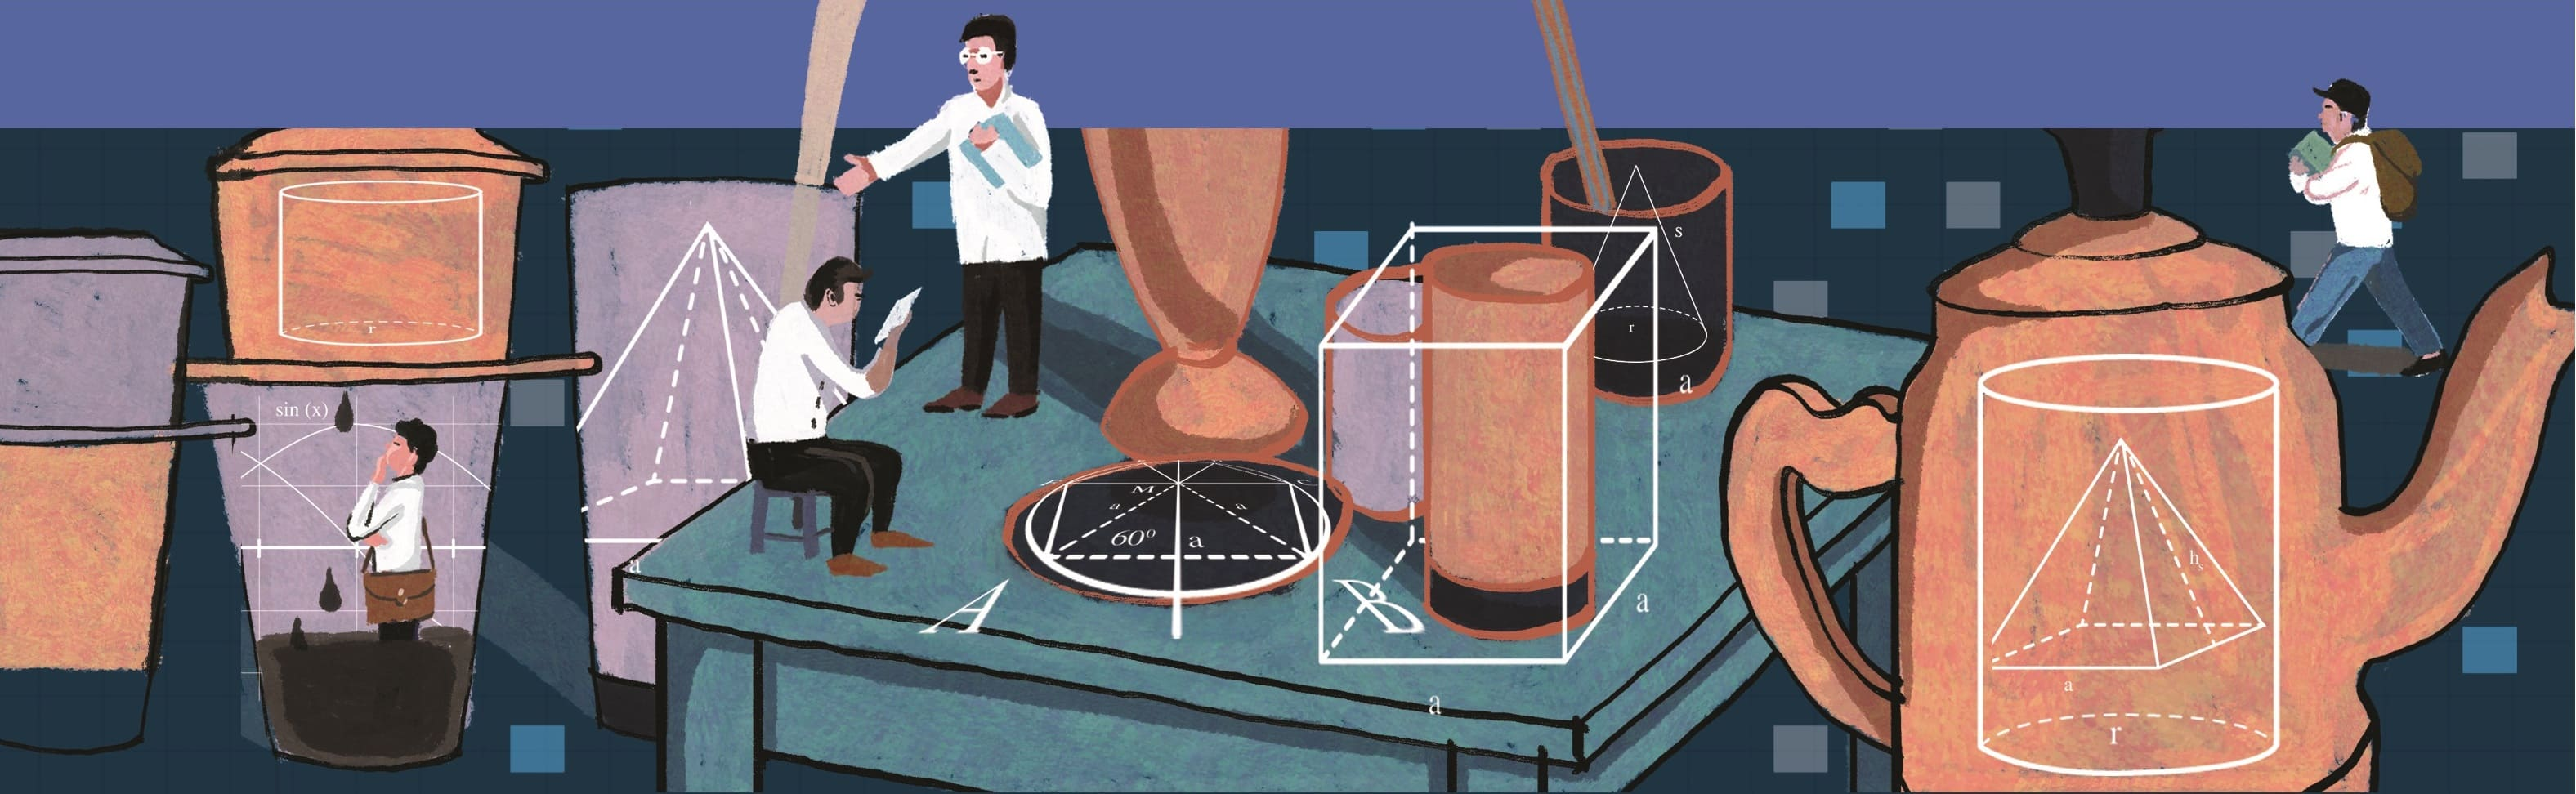
\includegraphics[width=19.3cm]{../bannerquantoan}}}
\AddToShipoutPicture*{\put(114,525){
\includegraphics[scale=1]{../tieude.pdf}}}
\centering
\endgroup
\vspace*{180pt}

\begin{multicols}{2}
	Ennio de Giorgi $(1928-1996)$ là một nhà toán học người Ý, người đã nghiên cứu các phương trình đạo hàm riêng và các nền tảng của toán học. Ennio theo học tại trường trung học ``G. Palmieri' ở quê nhà và bộc lộ những tài năng đặc biệt. Tuy nhiên, lúc ban đầu, mối quan tâm của ông không hướng tới toán học [$1$]:
	\vskip 0.01cm
	\begin{wrapfigure}{l}{0.45\linewidth}
		\vspace*{-10pt}
		\centering
		\captionsetup{labelformat= empty, justification=centering}
		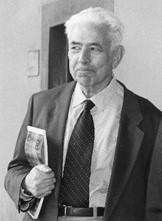
\includegraphics[width= 1\linewidth]{1}
		\caption{\small\textit{\color{quantoan}Ennio de Giorgi.}}
		\vspace*{-15pt}
	\end{wrapfigure}
	\textit{... khi còn nhỏ, tôi có sở thích đặc biệt trong việc mầy mò tìm ra lời giải cho những bài toán nhỏ, nhưng tôi cũng có niềm đam mê nhất định với việc thử nghiệm các thiết bị nhỏ -- các thí nghiệm, nếu không phải là của vật lý, thì là của thứ gọi là ``tiền vật lý".}
	\vskip 0.1cm
	Sau khi tốt nghiệp trung học năm $1946$, ông đến Rome để vào Đại học tại thủ đô, nhưng do đam mê các thiết bị, ông đã nhập học tại Khoa Kỹ thuật với ý định lấy bằng kỹ sư. Bất chấp việc quyết định chọn chủ đề nghiên cứu, De Giorgi đã khám phá ra niềm vui lúc đi học khi tìm ra cách chứng minh các định lý toán học khác với những chứng minh được viết trong sách giáo khoa. Đây chắc chắn là dấu hiệu ban đầu cho thấy tình yêu nghiên cứu của ông. Sau một năm học, Ennio quyết định rằng toán học chứ không phải kỹ thuật mới là môn học của mình [$1$]:
	\vskip 0.1cm
	\textit{Vào thời đó, các khóa học về toán học, kỹ thuật và vật lý đều giống nhau trong hai năm đầu tiên. Chính trong năm đầu tiên đó, tôi đã nhận ra rằng năng khiếu bẩm sinh của mình, trên tất cả, là về toán học.}
	\vskip 0.1cm
	Trong môn toán, De Giorgi theo học với Mauro Picone, người đã ảnh hưởng mạnh mẽ đến mình [$1$]:
	\vskip 0.1cm
	\textit{... tại Viện Toán học ở Rome, tôi đã học cùng và nhận bằng từ Giáo sư Picone, người với tư cách là một học giả, luôn trung thành với phong cách ``quý tộc" của những ngày đó, nhưng đồng thời là cũng là một người, trong thảo luận về các vấn đề khoa học, đã luôn hoàn toàn cởi mở. Tôi nhớ ông đã nói: ``Hãy nhớ rằng khi chúng ta nói về các vấn đề khoa học, bạn hoàn toàn có quyền nói với tôi rằng tôi đã nhầm, bởi vì chúng ta bình đẳng trước khoa học." Vì vậy, ông cực kỳ phóng khoáng trong đối thoại khoa học nhưng hoàn toàn tôn trọng kỷ luật và phong tục học thuật thời đó.} 
	\vskip 0.1cm
	De Giorgi hoàn thành chương trình học đại học vào năm $1950$ khi ông được nhận bằng tốt nghiệp. Sau đó, ông bắt đầu công việc nghiên cứu tại Viện Castelnuovo ở Rome, nơi ông là trợ lý cho Mauro Picone. Jacques--Louis Lions và François Murat viết trong [$4$] (xem thêm [$3$]):
	\vskip 0.1cm
	\textit{Vị Giáo sư và anh sinh viên đó thực sự là một sự kết hợp kỳ lạ: một người là người theo chủ nghĩa cổ điển, ăn mặc nghiêm túc và sang trọng; người kia, không chính thống, luôn đội xùm xụp chiếc mũ nồi kỳ khôi của mình. Nhưng M. Picone, một nhà quan sát dày dạn kinh nghiệm về sự phát triển của khoa học, đã biết cách phát hiện tài năng; ông ấy sớm thừa nhận khả năng đặc biệt của E. De Giorgi. Người trợ lý trẻ được giải phóng khỏi mọi ràng buộc và làm việc theo ý mình một cách nhàn nhã, nhưng cuối cùng lại hiệu quả đến kinh ngạc.}
		\begin{figure}[H]
		\vspace*{-5pt}
		\centering
		\captionsetup{labelformat= empty, justification=centering}
		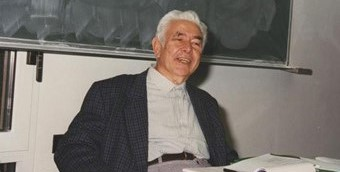
\includegraphics[width= 1\linewidth]{2}
		%		\caption{\small\textit{\color{}.}}
		\vspace*{-15pt}
	\end{figure}
	De Giorgi tham dự các bài giảng của Caccioppoli về lý thuyết độ đo hình học, nhưng vào thời điểm này ông đã có những ý tưởng của riêng mình về cách giải quyết các vấn đề về mặt cực tiểu. Dưới ảnh hưởng của các phương pháp mà Caccioppoli đã phát triển, De Giorgi tiếp tục phát triển các kỹ thuật mới trong lý thuyết độ đo hình học và ông áp dụng kết quả của mình vào phép tính biến phân để chứng minh định lý chính của ông cho hầu hết các mặt cực tiểu. Công trình đầu tiên của De Giorgi trong lý thuyết độ đo hình học về chủ đề các tập có chu vi hữu hạn mà ông gọi vào năm $1958$ là tập hợp Caccioppoli, theo tên người thầy và người bạn của mình. Định nghĩa của ông, áp dụng một số công cụ giải tích quan trọng và định lý De Giorgi cho các tập hợp, đã thiết lập một công cụ mới cho lý thuyết tập hợp cũng như các công trình của riêng ông. Thành tựu này không chỉ mang lại cho Ennio sự công nhận ngay lập tức mà còn thể hiện khả năng giải quyết các vấn đề bằng cách sử dụng hoàn toàn các phương pháp mới và hiệu quả, mặc dù đã được hình thành trước đó, nhưng có thể được sử dụng với độ chính xác cao hơn như  đã được thể hiện trong các công trình nghiên cứu của ông. Công trình sớm nhất  của ông nhằm mục đích phát triển một lý thuyết về tính chính quy cho các siêu  mặt cực tiểu, đã vĩnh viễn thay đổi cách chúng ta nhìn nhận lý thuyết cao cấp về các bề mặt cực tiểu và phép tính biến phân. Cùng với Enrico Bombieri và Enrico Giusti, ông đưa ra lời giải cho bài toán Bernstein về  mặt cực tiểu cho số chiều $n= 8$  vào năm $1969$, nhờ đó Bombieri được trao Giải thưởng Fields  vào năm $1974$.
	\vskip 0.1cm
	Năm $1955$ De Giorgi đã đưa ra một ví dụ quan trọng cho thấy tính không duy nhất nghiệm của bài toán Cauchy đối với các phương trình đạo hàm riêng dạng parabolic có các hệ số thỏa mãn các điều kiện chính quy nhất định. Trong năm tiếp theo, ông đã chứng minh được điều ngày nay mang tên ``Định lý De Giorgi" liên quan đến tính liên tục Hölder của nghiệm của phương trình đạo hàm riêng dạng elliptic cấp hai. Những kết quả này cũng tương tự với những kết quả được Nash chứng minh vào cùng một thời điểm. De Giorgi nói:
	\vskip 0.1cm
	\textit{Nash và tôi đã chứng minh cùng một định lý, hay nói đúng hơn là hai định lý rất gần nhau. Từ định lý Nash người ta có thể suy ra nhiều hay ít ngay lập tức định lý của tôi, theo một cách chứng minh hoàn toàn khác. Do đó, theo kinh nghiệm của tôi, việc khám phá một định lý có thể được thực hiện bởi những người khác nhau, như thể nó đã ở đó sẵn để chờ ai đó khám phá ra nó, và phát biểu của định lý đó sẽ luôn giống nhau. Tuy nhiên, phép chứng minh được sáng tạo ra có thể sẽ khác nhau rất nhiều tùy theo nhà toán học tìm ra nó.}
	\vskip 0.1cm
	Năm $1958$ De Giorgi được bổ nhiệm làm Trưởng khoa Giải tích Toán học tại Đại học Messina và ông đã nhận nhiệm vụ vào tháng $12$ năm đó. Tuy nhiên, ông giữ chức vụ này chưa đầy một năm vì đã được Alessandro Faedo tiếp cận, người đã thuyết phục ông chuyển đến Scuola Normale Superiore tại Pisa. Vào mùa thu năm $1959$ De Giorgi chuyển đến Pisa để đảm nhận chức vụ Trưởng khoa Giải tích Toán học.
	\vskip 0.1cm
	\textit{Trong gần bốn mươi năm, ông sống ở đó, dạy học ở đó và luôn là nguồn cảm hứng thường xuyên cho ngôi trường toán học mà ông thành lập. Luôn vui vẻ, luôn sẵn sàng, ông thích những cuộc tranh luận kéo dài với các học trò của mình, trong đó ông sẽ đưa ra những ý tưởng độc đáo và đề xuất những phỏng đoán hoặc phác thảo những dòng chứng minh.}
	\vskip 0.05cm
	De Giorgi đã nhận được nhiều sự tôn vinh vì những đóng góp toán học xuất sắc của mình, trong đó có Giải Caccioppoli năm $1960$, Giải thưởng Quốc gia của Viện Lincei (Accademia dei Lincei, Italia) năm $1973$, và Giải thưởng Wolf (Israel) năm $1990$, bằng tiến sỹ danh dự về Toán học của Đại học Paris năm $1983$, và về Triết học của Đại học Lecce năm $1992$. Ông được bầu vào nhiều Viện hàn lâm bao gồm:  Viện Accademia dei Lincei, Viện Hàn lâm Khoa học Giáo hoàng (Pontifical Academy of Sciences), Viện Hàn lâm Khoa học Turin, Viện Khoa học và Văn học Lombard, Académie des Sciences ở Paris và Viện Hàn lâm Khoa học Quốc gia Hoa Kỳ.
	\vskip 0.1cm
	Bên cạnh những thành công trong toán học của ông. Ennio là một người có tín ngưỡng và thường nói về niềm tin của mình [$2$]:
	\vskip 0.1cm
	\textit{Sách Châm ngôn, một trong những cuốn sách cổ nhất của Kinh thánh,  có nói rằng Thông thái đã ở cùng Thượng Đế khi Ngài tạo ra thế giới và rằng Thông thái sẽ được tìm thấy bởi những người tìm kiếm và yêu mến nó. Toán học là một trong những biểu hiện quan trọng nhất của tình yêu dành cho Thông thái.}
	\begin{figure}[H]
			\vspace*{-5pt}
			\centering
			\captionsetup{labelformat= empty, justification=centering}
			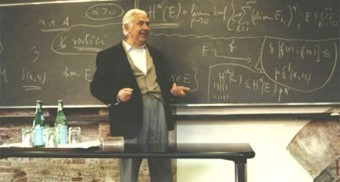
\includegraphics[width= 1\linewidth]{3}
			%		\caption{\small\textit{\color{}.}}
			\vspace*{-15pt}
		\end{figure}
	Ông cũng là một người nhiệt tình ủng hộ hòa bình và hữu nghị giữa các dân tộc và thể hiện điều này bằng những hoạt động tích cực của mình, ông phát biểu [$2$]:
	\vskip 0.1cm
	\textit{... bản Tuyên Ngôn Quốc Tế Nhân Quyền có Điều khoản nói về nền giáo dục khuyến khích không chỉ sự khoan dung mà còn cả sự hiểu biết và tình hữu nghị giữa các quốc gia khác nhau và các nhóm tôn giáo khác nhau. Hiểu biết và tình bạn là hai khái niệm thường bị lãng quên khi nói về lòng khoan dung. Sự khoan dung một cách trong sáng và đầy cảm tính là không đủ; chỉ khi được kết hợp với sự hiểu biết và tình bạn thì nó mới thực sự cho phép hoạt động của con người được phát triển. Đặc biệt, các ngành khoa học không thể tiến lên nếu không có sự hiểu biết và tình bạn giữa tất cả các nhà khoa học.}
	\vskip 0.1cm
	\textbf{\color{quantoan}Tài liệu tham khảo}
	\vskip 0.1cm
	[$1$]	L. Ambrosio, G. Dal Maso, M. Forti, M. Miranda and S. Spagnolo, Ennio De Giorgi (Italian), \textit{Boll. Unione Mat. Ital. Sez. B Artic. Ric. Mat.} ($8$) $2$ ($1$) ($1999$), $3-31$.
	\vskip 0.1cm
	[$2$]	M. Emmer (trs.), Interview with Ennio De Giorgi, \textit{Notices Amer. Math. Soc.} $44$ ($9$) ($1997$), $1097-1101$. \url{http://www.ams.org/notices/199709/emmer.pdf}
	\vskip 0.1cm
	[$3$]	J--L. Lions and F. Murat, Ennio De Giorgi ($1928-1996$) (French), \textit{Gaz. Math}. No. $71$ ($1997$), $30-34$.
	\vskip 0.1cm
	$[4]$	J--L. Lions and F. Murat, Ennio De Giorgi ($1928-1996$), \textit{Notices Amer. Math. Soc}. $44$ ($9$) ($1997$), $1095-1096$. \url{http://www.ams.org/notices/199709/murat.pdf}
\end{multicols}
\newpage
\begingroup
\AddToShipoutPicture*{\put(132,678){
\includegraphics[scale=1]{../tieude2.pdf}}}
\centering
\endgroup
\blfootnote{$^1$\color{quantoan}Viện Vật lý.}
\vspace*{30pt}

\begin{multicols}{2}
	Richard Feynman ($1918-1988$, Mỹ) nổi tiếng là người trung thực không khoan nhượng và đam mê đến tận cùng. Về tính trung thực, người ta hay nhắc đến vụ ông trình diễn trực tiếp trên TV một ``thí nghiệm nhỏ", bỏ vòng cao su vào cốc nước đá, minh chứng rằng cao su mất tính đàn hồi ở nhiệt độ thấp, qua đó chỉ ra nguyên nhân dẫn đến thảm họa tàu vũ trụ con thoi ``Challenger", vạch trần chiến dịch tung hỏa mù của NASA về nguyên nhân của thảm họa này. Để công bố với người dân Mỹ sự thật ấy, Feynman đã phải vượt qua sức ép khủng khiếp từ các cơ quan công quyền Mỹ, trong đó có CIA và NASA. 
	\begin{figure}[H]
			\vspace*{-5pt}
			\centering
			\captionsetup{labelformat= empty, justification=centering}
			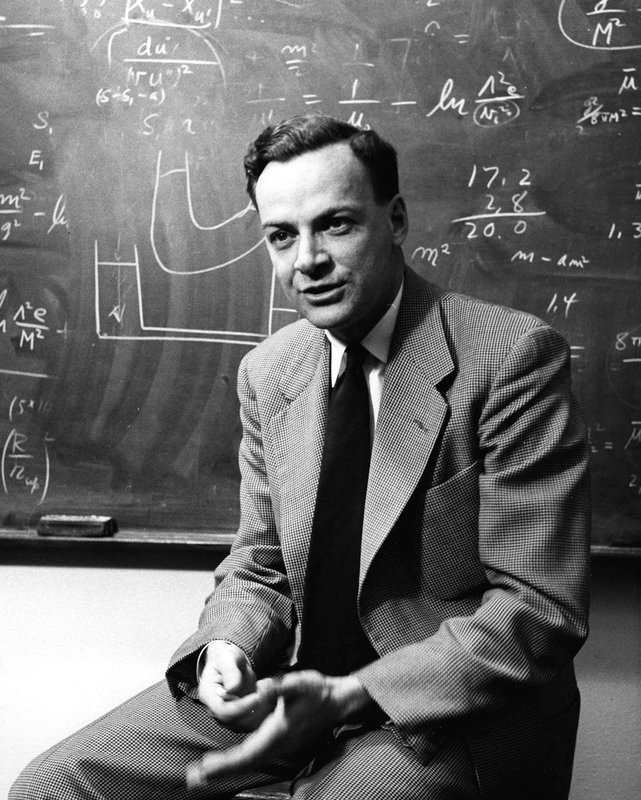
\includegraphics[width= 1\linewidth]{1a}
			\caption{\small\textit{\color{quantoan}Richard Feynman (ảnh từ bộ sưu tập của Viện Công nghệ California -- CalTech).}}
			\vspace*{-10pt}
		\end{figure}
	Feynman lắm đam mê. Đam mê vật lý, Feynman nhận giải Nobel Vật lý năm $1965$. Đam mê chơi trống, vở ba--lê do ông đệm trống nhận giải nhất trong cuộc thi ba--lê toàn nước Mỹ và giải nhì trong cuộc thi quốc tế tại Paris. Đam mê vẽ, ông đã có triển lãm tranh riêng. Không rõ ông biết những ngôn ngữ nào, chỉ biết thăm Brazil ông dạy bằng tiếng Bồ, thăm Nhật ông giao du bằng tiếng Nhật. Rồi có lần bạn bè định ``cho ông một vố", họ nhờ một cô Hoa kiều đón tiếp ông bằng tiếng Trung, Feynman đáp lại và cô ấy kêu trời, vì ông nói tiếng Quảng Đông, còn cô chỉ nói tiếng Bắc Kinh. Rất nhiều ``đam mê" kiểu như vậy được kể trong cuốn ``Feynman, chuyện thật như đùa" (NXB Trẻ) và hầu như tất cả đều có kết cục mỹ mãn, kiểu như giải Nobel. Có thể bạn nghĩ chắc ông này ``con nhà nòi", học ``trường quốc tế" từ nhỏ! Xin thưa, bố của Feynman là người bán rong bán quần áo, còn mẹ thì nội trợ. 
	\begin{figure}[H]
			\vspace*{-5pt}
			\centering
			\captionsetup{labelformat= empty, justification=centering}
			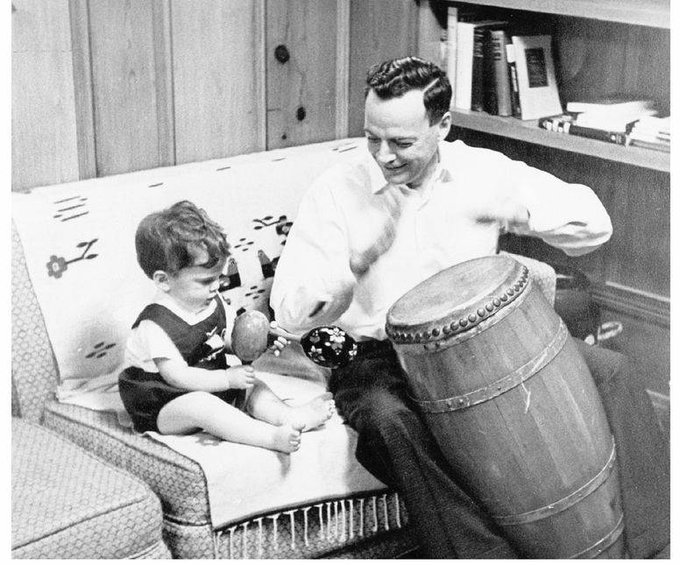
\includegraphics[width= 1\linewidth]{2a}
			\caption{\small\textit{\color{quantoan}Feynman chơi trống bên con trai (ảnh từ Internet).}}
			\vspace*{-10pt}
		\end{figure}
	Ông chơi trống bongo cực giỏi, nhưng chưa bao giờ học nhạc lý. Ông vốn vẽ rất kém, tự nhận chẳng thể vẽ nổi cái gì ngoại trừ cái kim tự tháp chỉ gồm mấy đường thẳng. Để học vẽ, Feynman ``đổi công" với một họa sỹ: ông dạy vật lý cho họa sỹ còn họa sỹ dạy vẽ cho ông. Hãy tưởng tượng một giáo sư nổi tiếng thế giới ngồi trong lớp vẽ cùng các cháu $8-9$ tuổi học cách gọt bút chì. Đam mê như thế chỉ có ở Feynman. Và, với ông đam mê chính là nguồn cội của thành công, chứ chẳng phải ``con nhà nòi" hay ``trường quốc tế" nào cả. Tiền bạc và chứng chỉ đầy người, mà không đam mê gì, thì làm sao có thành quả! 
	\begin{figure}[H]
			\vspace*{-5pt}
			\centering
			\captionsetup{labelformat= empty, justification=centering}
			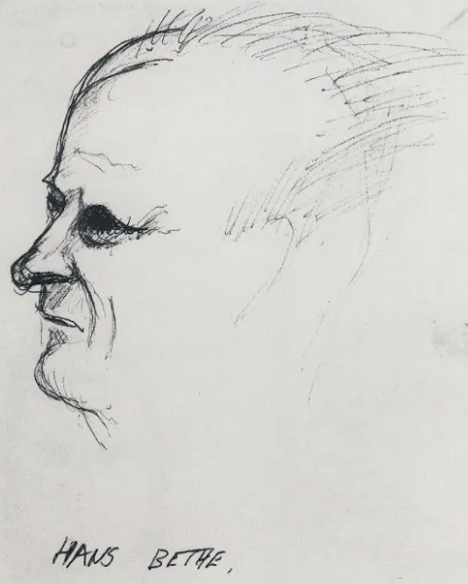
\includegraphics[width= 1\linewidth]{3a}
			\caption{\small\textit{\color{quantoan}Feyman vẽ Hans Bethe (giải Nobel Vật lý $1967$).}}
			\vspace*{-10pt}
		\end{figure}
	Duy có đam mê cuối cùng, Feynman đã không kịp nhìn thấy những gì mình muốn, trước khi về cõi vĩnh hằng. Đó là ``Cuộc phiêu lưu cuối cùng của Feynman"\footnote[2]{\color{quantoan}Xem thêm: Cuộc phiêu lưu cuối cùng của Feynman, in lần $2$, NXB Trẻ, $2023$.}. Cuộc phiêu lưu khởi đầu bằng một con tem có xuất xứ từ một nơi gọi là Tannu Tuva, mà Feynman có được từ khi còn nhỏ. Cái tên ``Tuva" xa lạ nằm yên trong đầu Feynman, cho đến một ngày hè $1977$ nó trở thành mục tiêu cho ``cuộc phiêu lưu" kéo dài hơn $10$ năm cuối của cuộc đời ông. Tôi cược là nhiều bạn chưa biết Tuva là địa danh nào và ở đâu. Để đỡ tra cứu, xin ``bật mí" ngay: đó là tên một quốc gia nhỏ nằm giáp phía Tây Bắc của Mông Cổ, vốn độc lập, nhưng đã sáp nhập vào Liên Xô cũ (và Nga ngày nay). Thủ đô của Tuva là Kyzyl. Tuva có gì đặc biệt mà khiến Feynman mê mệt đến vậy?
	\vskip 0.1cm
	Bạn có biết đâu là trọng tâm của châu Á (lục địa thôi chứ không tính các đảo)? Lấy tấm bìa cứng phẳng, vẽ lên đó bản đồ châu Á, cắt theo đường biên để được miếng bìa hình châu Á lục địa. Dùng một chiếc bút đầu nhọn chống phía dưới tấm bìa, di di đầu bút, để tìm vị trí mà tấm bìa nằm cân bằng trên chiếc bút thẳng đứng. Vị trí đó rơi vào Kyzyl, trọng tâm của châu Á. Tất nhiên, các nhà khoa học xác định điểm này bằng các phương pháp chính xác hơn, và ngày nay ở Kyzyl có tấm bia lớn khẳng định vị trí đặc biệt của thành phố này. Nhưng, chỉ chừng ấy thì không đủ để Feynman mất tới cả chục năm tìm cách tới thăm Tuva.
	\begin{figure}[H]
			\vspace*{-5pt}
			\centering
			\captionsetup{labelformat= empty, justification=centering}
			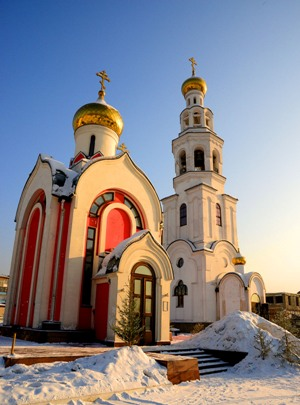
\includegraphics[width= 1\linewidth]{4a}
			\caption{\small\textit{\color{quantoan}Nhà thờ Phục sinh ở Kyzyl, Tuva (ảnh từ Internet).}}
			\vspace*{-10pt}
		\end{figure}
	Cái chính là ở quốc gia tí xíu bao bọc bởi những dãy núi cao ấy, thời gian gần như ngừng trôi: tất cả vẫn nguyên sơ như $500$ hay $1000$ năm trước. Thảo nguyên hoang dại. Những đàn tuần lộc hay bò Tây Tạng cũng dường như hoang dại. Cuộc sống du mục không thể tự nhiên hơn. Một nền văn hóa xa xưa và kỳ thú với kiểu hát hai giọng chỉ có ở Tuva, với thứ văn tự không thể tìm thấy trong bất cứ tự điển nào, với các tập tục rất lạ điều hành bởi các tù trưởng uy nghi và bí ẩn v.v. Tiếc là ít người biết Tuva, chứ không, người ta đã gọi quốc gia này là ``Thảo nguyên Xanh" cuối cùng của hành tinh Trái Đất (như Congo là Hành tinh Xanh cuối cùng). Đam mê Tuva, Feynman tìm đọc mọi tài liệu về Tuva, tìm hiểu văn tự Tuva, học cách hát của dân du mục Tuva, ăn mặc và trang trí như tù trưởng Tuva \ldots Và, nhất là, ông tìm mọi cách để có thể đến thăm Tuva.
	\vskip 0.1cm
	Đó là thời Chiến tranh Lạnh, lại nghe nói, gần Tuva có một cơ sở nghiên cứu bom nguyên tử, nên nơi đây là ``vùng cấm" với khách du lịch, nhất là khách nước ngoài. Thực ra, Viện Hàn lâm Khoa học Liên Xô sẵn sàng mời Feynman sang Moscow  đọc bài giảng rồi đi ``tham quan Kyzyl" theo kiểu mặc com--lê ở khách sạn có người bảo vệ v.v. Nhưng Feynman không thích như vậy, mà muốn tự mình mang ba--lô đến thảo nguyên, ngủ lều, uống sữa tuần lộc và hát hai giọng cùng dân bản xứ. Ấy thế cho nên ông mất cả chục năm tìm kiếm một giấy mời như mình muốn. Và, đầu tháng Ba $1988$, một giấy mời như thế đã gửi đến địa chỉ của Feynman, chỉ tiếc là hai tuần trước đó, vào ngày $15$ tháng Hai, ông đã ra đi mãi mãi, nên chỉ có thể trải nghiệm ``Cuộc phiêu lưu cuối cùng" của mình trong tâm trí và trái tim của những người ở lại. Không rõ, ở Thế giới bên kia Feynman đang đam mê gì?
\end{multicols}
%	\newpage
%
%	\thispagestyle{empty}
%	\begingroup 
%	\AddToShipoutPicture*{\put(0,0){\includegraphics[width=19.45cm]{QC}}}
%	\centering
%	\vspace*{0cm}
%	\endgroup
%	\newpage	
%	\pagestyle{empty}
%
%	\setcounter{figure}{0}
%	\thispagestyle{toancuabinone}
\pagestyle{toancuabi}
\everymath{\color{toancuabi}}
%\blfootnote{$^1$\color{toancuabi}Trường Liên cấp Hội nhập Quốc tế iSchool Quảng Trị.}
\graphicspath{{../toancuabi/pic/}}
\begingroup
\AddToShipoutPicture*{\put(0,616){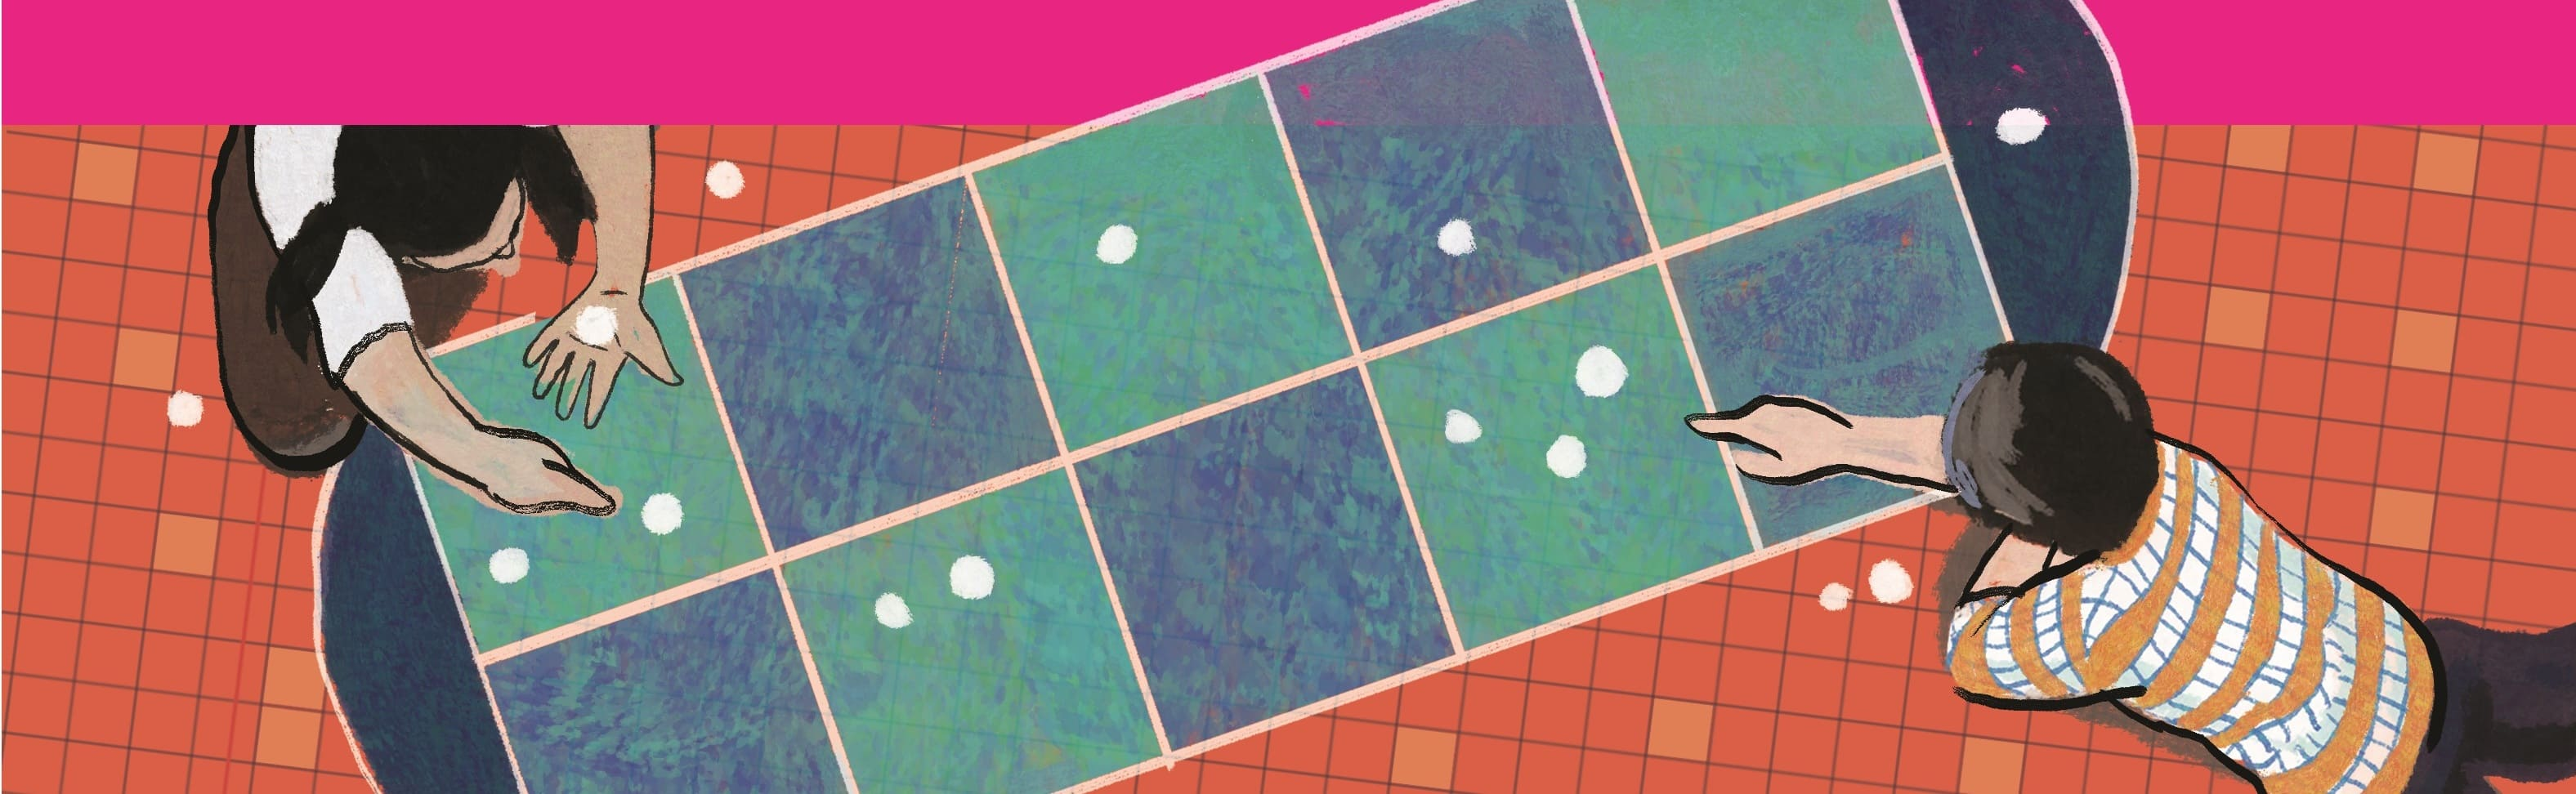
\includegraphics[width=19.3cm]{../bannertoancuabi}}}  
\AddToShipoutPicture*{\put(62,492){
\includegraphics[scale=1]{../tieude1.pdf}}}  
\centering
\endgroup
\vspace*{215pt} 

\definecolor{bulgarianrose}{rgb}{0.28, 0.02, 0.03}
\begin{multicols}{2}
	Câu lạc bộ toán học ``Unicorn Math Circle" (UMC) dành cho học sinh Tiểu học và THCS được Tạp chí Pi tổ chức từ năm $2019$, nhằm tìm kiếm và bồi dưỡng các học sinh có năng lực Toán học, tạo nguồn học sinh xuất sắc. Trong số này, tạp chí Pi giới thiệu đến bạn đọc đề thi tuyển sinh năm học $2023-2024$ dành cho các bạn học sinh lớp $4$.
	\vskip 0.1cm
	\textbf{\color{toancuabi}Bài $\pmb{1.}$} Dựa vào quy luật, hỏi hình nào trong số các hình $A$, $B$, $C$, $D$ là hình tiếp theo trong dãy sau:
	\begin{figure}[H]
		\vspace*{-5pt}
		\centering
		\captionsetup{labelformat= empty, justification=centering}
		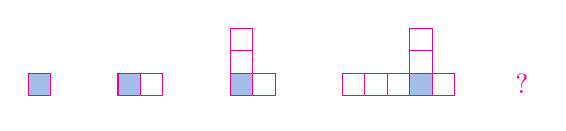
\begin{tikzpicture}[toancuabi,scale=0.285]
			\fill[cackithi!50] (-2,0) rectangle (-1,1);
			\fill[cackithi!50] (2,0) rectangle (3,1);
			\fill[cackithi!50] (7,0) rectangle (8,1);
			\fill[cackithi!50] (15,0) rectangle (16,1);
			\draw (-2,0) grid (-1,1);
			\draw (2,0) grid (4,1);
			\draw (7,0) grid (9,1);
			\draw (7,1) grid (8,3);
			\draw (12,0) grid (17,1);
			\draw (15,1) grid (16,3);
			\draw (20,0.5) node {$?$};
		\end{tikzpicture}

		\vspace*{10pt}
		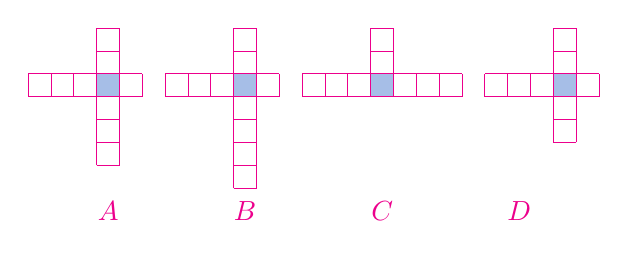
\begin{tikzpicture}[toancuabi,scale=0.29]
			\fill[cackithi!50] (3,0) rectangle (4,1);
			\fill[cackithi!50] (9,0) rectangle (10,1);
			\fill[cackithi!50] (15,0) rectangle (16,1);
			\fill[cackithi!50] (23,0) rectangle (24,1);
			\draw (0,0) grid (5,1);
			\draw (3,-3) grid (4,3);
			\draw (6,0) grid (11,1);
			\draw (9,-4) grid (10,3);
			\draw (12,0) grid (19,1);
			\draw (15, 1) grid (16,3);
			\draw (20,0) grid (25,1);
			\draw (23,-2) grid (24,3);
			
			\draw (3.5,-5) node{$A$};
			\draw (9.5,-5) node{$B$};
			\draw (15.5,-5) node{$C$};
			\draw (21.5,-5) node{$D$};
		\end{tikzpicture}
		\vspace*{-15pt}
	\end{figure}
	\textbf{\color{toancuabi}Bài $\pmb{2.}$} Một cặp số có hai chữ số như $18$ và $81$ được gọi là cặp \textit{bạn thân} vì chúng có chữ số hàng chục và chữ số hàng đơn vị đổi chỗ cho nhau. Hỏi có bao nhiêu cặp bạn thân mà tổng của chúng bằng $99$?
	\vskip 0.1cm
	\textbf{\color{toancuabi}Bài $\pmb{3.}$} Bạn Ngọc được tặng một thanh sô--cô--la hình trái tim. Mỗi ô vuông có trọng lượng $8$g. Hỏi thanh sô--cô--la có khối lượng bằng bao nhiêu?
	\begin{figure}[H]
		\vspace*{-5pt}
		\centering
		\captionsetup{labelformat= empty, justification=centering}
		\begin{tikzpicture}[scale=0.6]
			\clip (0,0) - ++(0,2) - ++(2,4) - ++(4,2) - ++(6,4) - ++(8,2) - ++(8,0) - ++(4,-4) -- cycle;;
			\draw[fill=bulgarianrose!90] (0,0) - ++(0,2) - ++(2,4) - ++(4,2) - ++(6,4) - ++(8,2) - ++(8,0) - ++(4,-4) -- cycle;
			\draw (0,0) - ++(0,2) - ++(2,4) - ++(4,2) - ++(6,4) - ++(8,2) - ++(8,0) - ++(4,-4) -- cycle;
			\draw (0,-4) grid (8,4);
		\end{tikzpicture}
		\vspace*{-5pt}
	\end{figure}
	\textbf{\color{toancuabi}Bài $\pmb{4.}$} Trong hình vẽ sau, mỗi miền được tô $1$ màu, không có $2$ miền nào cùng màu. Có bao nhiêu miền nằm trong ít nhất $3$ hình tròn?	 
	\begin{figure}[H]
		\vspace*{-5pt}
		\centering
		\captionsetup{labelformat= empty, justification=centering}
		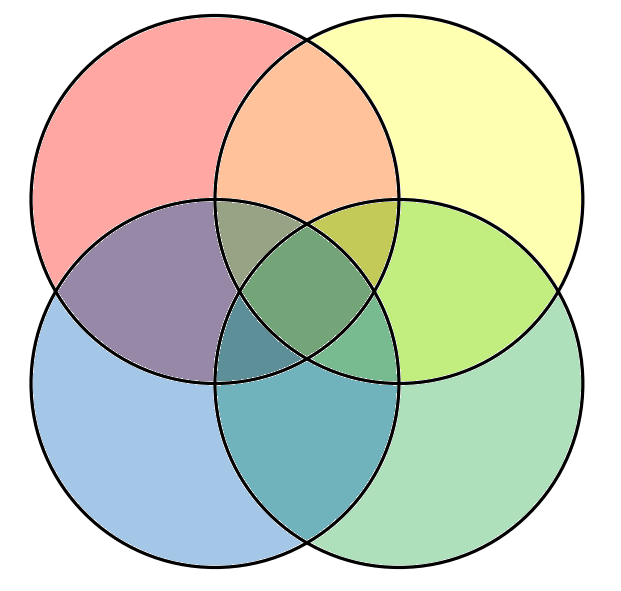
\includegraphics[width= 0.65\linewidth]{2}
%		\caption{\small\textit{\color{}}}
		\vspace*{-5pt}
	\end{figure}
	\textbf{\color{toancuabi}Bài $\pmb{5.}$} Số $1995$ được xếp bằng các que diêm như hình dưới đây. An dịch chuyển đúng $1$ que diêm để nhận được số lớn nhất có thể. Hỏi số đó bằng bao nhiêu?
	\begin{figure}[H]
		\vspace*{-5pt}
		\centering
		\captionsetup{labelformat= empty, justification=centering}
		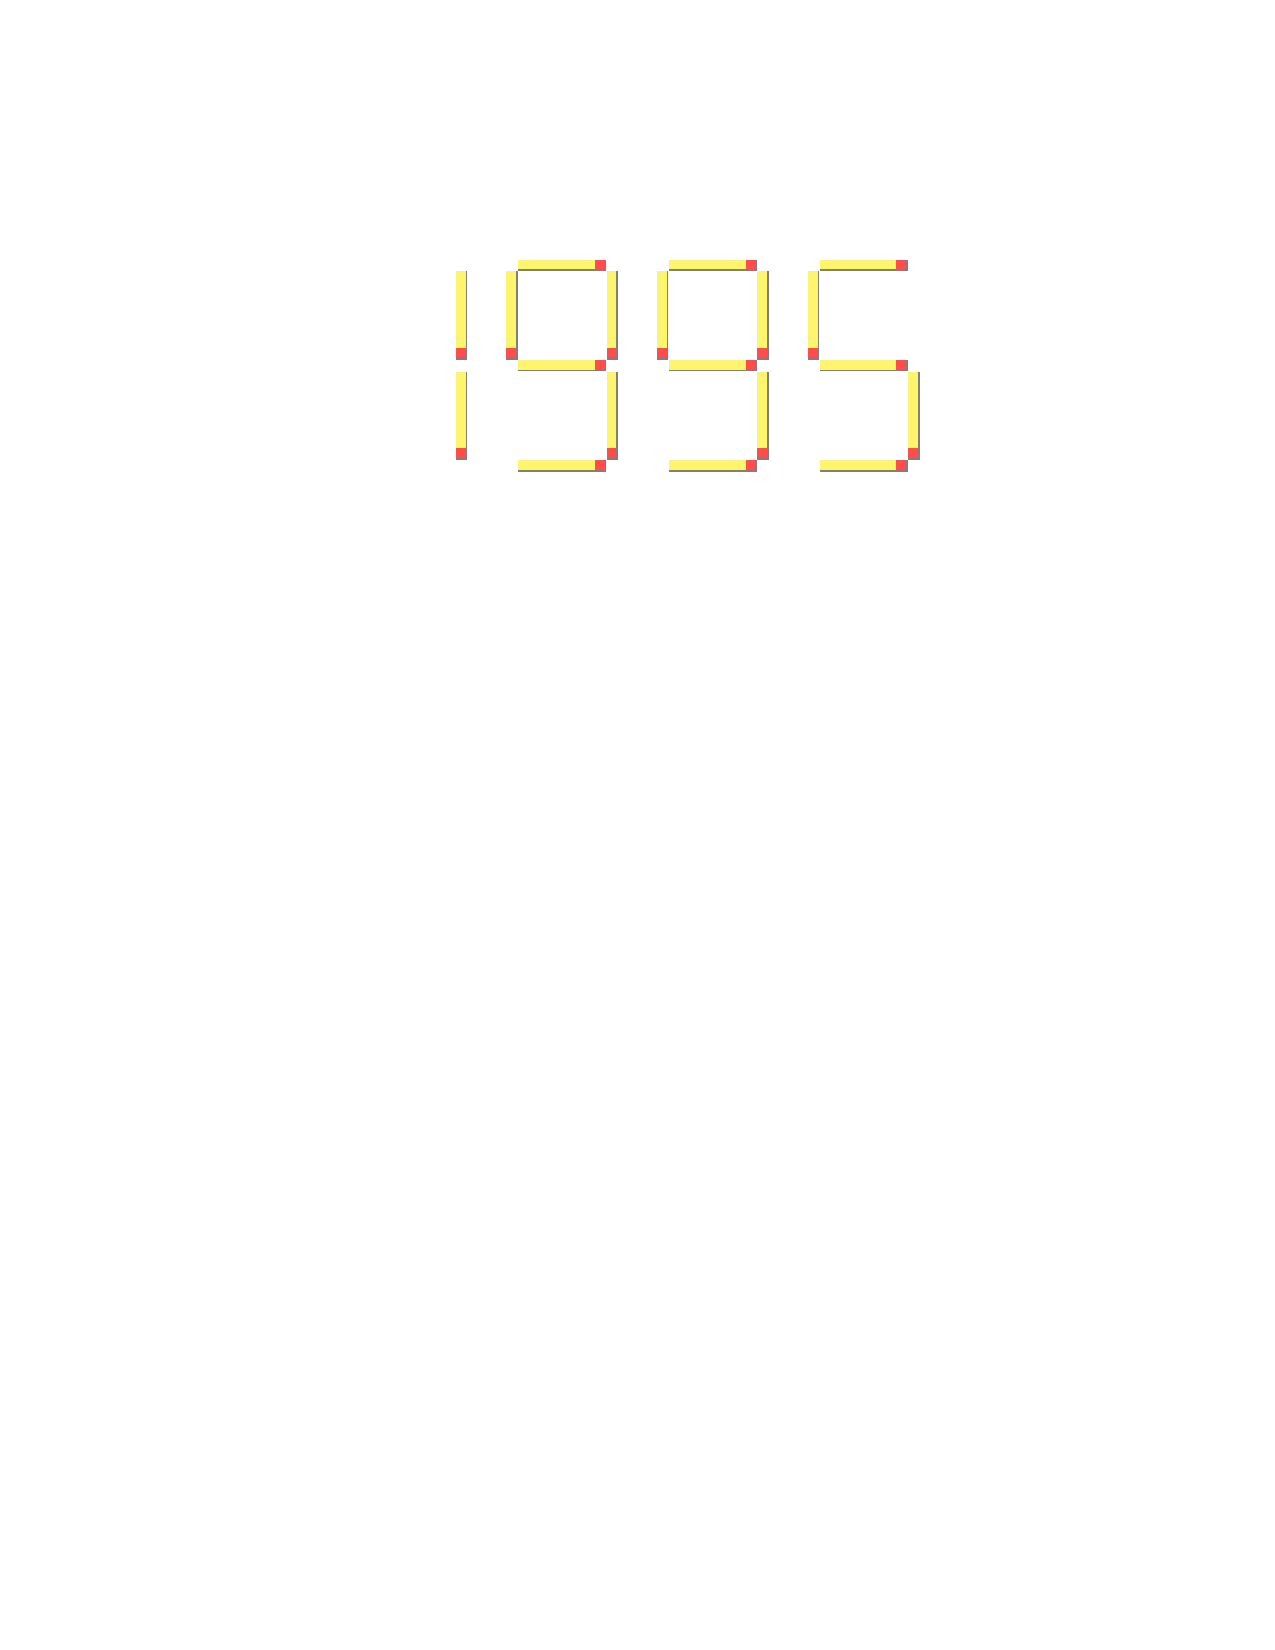
\includegraphics[width= 1\linewidth]{3}
%		\caption{\small\textit{\color{}}}
		\vspace*{-15pt}
	\end{figure}
	\textbf{\color{toancuabi}Bài $\pmb{6.}$} Như hình vẽ, có $9$ ô vuông nhỏ, vẽ một đường thẳng, hỏi đường thẳng này đi qua nhiều nhất bao nhiêu ô vuông nhỏ?
	\begin{figure}[H]
		\vspace*{-5pt}
		\centering
		\captionsetup{labelformat= empty, justification=centering}
		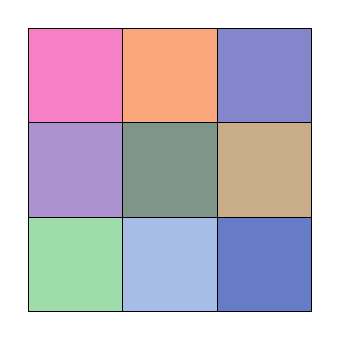
\begin{tikzpicture}[scale=1.2]
			\draw[fill=diendantoanhoc!50] (0,0) rectangle (1,1);
			\draw[fill=gocco!50] (0,1) rectangle (1,2);
			\draw[fill=toancuabi!50] (0,2) rectangle (1,3);
			\draw[fill=cackithi!50] (1,0) rectangle (2,1);
			\draw[fill=thachthuctoanhoc!50] (1,1) rectangle (2,2);
			\draw[fill=duongvaotoanhoc!50] (1,2) rectangle (2,3);
			\draw[fill=quantoan!80] (2,0) rectangle (3,1);
			\draw[fill=lichsutoanhoc!50] (2,1) rectangle (3,2);
			\draw[fill=timhieukhoahoc!60] (2,2) rectangle (3,3);
			\draw (0,0) grid (3,3);
		\end{tikzpicture}
		\vspace*{-5pt}
	\end{figure}
	\textbf{\color{toancuabi}Bài $\pmb{7.}$} Trong hình vẽ bên dưới, hình ngôi sao lớn được chia thành các hình tam giác có chu vi bằng $7$, các hình tứ giác có chu vi bằng $18$ và một hình ngôi sao nhỏ có chu vi bằng $3$. Tìm chu vi của hình ngôi sao lớn ban đầu.
	\begin{figure}[H]
		\vspace*{-5pt}
		\centering
		\captionsetup{labelformat= empty, justification=centering}
		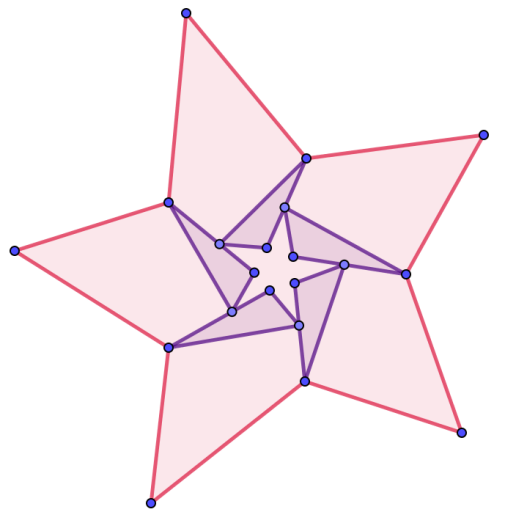
\includegraphics[width= 0.7\linewidth]{5}
%		\caption{\small\textit{\color{}}}
%		\vspace*{-10pt}
	\end{figure}
	\textbf{\color{toancuabi}Bài $\pmb{8.}$} Trong siêu thị có sự kiện ra mắt một loại kem mới, để quảng cáo loại kem này, họ cho phép cứ $2$ cái vỏ kem đổi được $1$ cây kem, bạn Bảo Châu mua $10$ que kem, vậy bạn ấy thực sự có thể ăn được nhiều nhất bao nhiêu que kem?
	\vskip 0.1cm
	\textbf{\color{toancuabi}Bài $\pmb{9.}$} Một hình vuông to được chia thành các hình vuông nhỏ hơn với nhiều kích cỡ, trong đó một số được tô màu hồng như hình vẽ. Biết diện tích phần màu trắng của hình vuông là $180$. Tìm diện tích phần màu hồng của hình vuông.
	\begin{figure}[H]
	\vspace*{-5pt}
	\centering
	\captionsetup{labelformat= empty, justification=centering}
	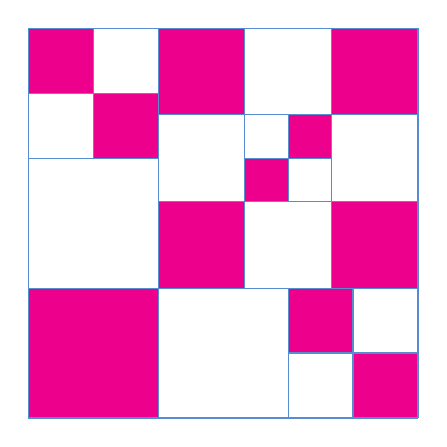
\begin{tikzpicture}[scale=0.55, cackithi]
		\fill[fill=toancuabi] (-2.,7.) -- (-2.,5.5) -- (-0.5,5.5) -- (-0.5,7.) -- cycle;
		\fill[fill=toancuabi] (-0.5,5.5) -- (-0.5,4.) -- (1.,4.) -- (1.,5.5) -- cycle;
		\fill[fill=toancuabi] (1.,7.) -- (1.,5.) -- (3.,5.) -- (3.,7.) -- cycle;
		\fill[fill=toancuabi] (5.,7.) -- (5.,5.) -- (7.,5.) -- (7.,7.) -- cycle;
		\fill[fill=toancuabi] (4.,5.) -- (4.,4.) -- (5.,4.) -- (5.,5.) -- cycle;
		\fill[fill=toancuabi] (3.,4.) -- (3.,3.) -- (4.,3.) -- (4.,4.) -- cycle;
		\fill[fill=toancuabi] (5.,3.) -- (5.,1.) -- (7.,1.) -- (7.,3.) -- cycle;
		\fill[fill=toancuabi] (1.,3.) -- (1.,1.) -- (3.,1.) -- (3.,3.) -- cycle;
		\fill[fill=toancuabi] (4.,1.) -- (4.,-0.5) -- (5.5,-0.5) -- (5.5,1.) -- cycle;
		\fill[fill=toancuabi] (5.5,-0.5) -- (5.5,-2.) -- (7.,-2.) -- (7.,-0.5) -- cycle;
		\fill[fill=toancuabi] (-2.,1.) -- (-2.,-2.) -- (1.,-2.) -- (1.,1.) -- cycle;
		\draw  (3.,5.)-- (5.,5.);
		\draw  (5.,5.)-- (5.,3.);
		\draw  (5.,3.)-- (3.,3.);
		\draw  (3.,3.)-- (3.,5.);
		\draw  (4.,5.)-- (4.,3.);
		\draw  (3.,4.)-- (5.,4.);
		\draw  (7.,5.)-- (7.,3.);
		\draw  (7.,3.)-- (5.,3.);
		\draw  (3.,5.)-- (1.,5.);
		\draw  (1.,5.)-- (1.,3.);
		\draw  (1.,3.)-- (3.,3.);
		\draw  (1.,3.)-- (1.,1.);
		\draw  (1.,1.)-- (7.,1.);
		\draw  (7.,1.)-- (7.,3.);
		\draw  (5.,3.)-- (5.,1.);
		\draw  (3.,3.)-- (3.,1.);
		\draw  (1.,5.)-- (1.,7.);
		\draw  (1.,7.)-- (7.,7.);
		\draw  (7.,7.)-- (7.,5.);
		\draw  (5.,5.)-- (5.,7.);
		\draw  (3.,5.)-- (3.,7.);
		\draw  (1.,7.)-- (-2.,7.);
		\draw  (-2.,7.)-- (-2.,1.);
		\draw  (1.,4.)-- (-2.,4.);
		\draw  (-2.,-2.)-- (7.,-2.);
		\draw  (7.,-2.)-- (7.,1.);
		\draw  (4.,1.)-- (4.,-2.);
		\draw  (-2.,7.)-- (-2.,5.5);
		\draw  (-2.,5.5)-- (-0.5,5.5);
		\draw  (-0.5,5.5)-- (-0.5,7.);
		\draw  (-0.5,7.)-- (-2.,7.);
		\draw  (-0.5,5.5)-- (-0.5,4.);
		\draw  (-0.5,4.)-- (1.,4.);
		\draw  (1.,4.)-- (1.,5.5);
		\draw  (1.,5.5)-- (-0.5,5.5);
		\draw  (1.,7.)-- (1.,5.);
		\draw  (1.,5.)-- (3.,5.);
		\draw  (3.,5.)-- (3.,7.);
		\draw  (3.,7.)-- (1.,7.);
		\draw  (5.,7.)-- (5.,5.);
		\draw  (5.,5.)-- (7.,5.);
		\draw  (7.,5.)-- (7.,7.);
		\draw  (7.,7.)-- (5.,7.);
		\draw  (4.,5.)-- (4.,4.);
		\draw  (4.,4.)-- (5.,4.);
		\draw  (5.,4.)-- (5.,5.);
		\draw  (5.,5.)-- (4.,5.);
		\draw  (3.,4.)-- (3.,3.);
		\draw  (3.,3.)-- (4.,3.);
		\draw  (4.,3.)-- (4.,4.);
		\draw  (4.,4.)-- (3.,4.);
		\draw  (5.,3.)-- (5.,1.);
		\draw  (5.,1.)-- (7.,1.);
		\draw  (7.,1.)-- (7.,3.);
		\draw  (7.,3.)-- (5.,3.);
		\draw  (1.,3.)-- (1.,1.);
		\draw  (1.,1.)-- (3.,1.);
		\draw  (3.,1.)-- (3.,3.);
		\draw  (3.,3.)-- (1.,3.);
		\draw  (4.,1.)-- (4.,-0.5);
		\draw  (4.,-0.5)-- (5.5,-0.5);
		\draw  (5.5,-0.5)-- (5.5,1.);
		\draw  (5.5,1.)-- (4.,1.);
		\draw  (5.5,-0.5)-- (5.5,-2.);
		\draw  (5.5,-2.)-- (7.,-2.);
		\draw  (7.,-2.)-- (7.,-0.5);
		\draw  (7.,-0.5)-- (5.5,-0.5);
		\draw  (-2.,1.)-- (-2.,-2.);
		\draw  (-2.,-2.)-- (1.,-2.);
		\draw  (1.,-2.)-- (1.,1.);
		\draw  (1.,1.)-- (-2.,1.);
	\end{tikzpicture}
	\vspace*{-5pt}
	\end{figure}
	\textbf{\color{toancuabi}Bài $\pmb{10.}$} Hai bạn Nam và Dương đi chợ sách và nhìn thấy cuốn tạp chí Pi. Nam muốn mua $1$ cuốn nhưng thiếu $12$ nghìn đồng. Dương muốn mua $1$ cuốn nhưng thiếu $23$ nghìn đồng. Nếu $2$ bạn chung tiền mua thì vừa đủ mua $1$ cuốn. Hỏi cuốn tạp chí Pi giá bao nhiêu tiền?
	\end{multicols}
	\newpage
	\begin{multicols}{2}
	\textbf{\color{toancuabi}Lời giải.}
	\vskip 0.1cm
	\textbf{\color{toancuabi}Bài $\pmb{1.}$} Ta thấy nếu lấy ô vuông được tô màu làm tâm, thì theo ngược chiều kim đồng hồ số các ô vuông kề với tâm sẽ tăng dần: $1,2,3,4$. Do đó hình $B$ là hình tiếp theo trong dãy.
	\vskip 0.1cm
	\textbf{\color{toancuabi}Bài $\pmb{2.}$} Ta có thể thấy ngay cặp số bạn thân có tổng bằng $99$ thì mỗi số trong cặp có tổng chữ số hàng chục và hàng đơn vị bằng $9$. Do $9 = 1+8 = 2+7 = 3+6 = 4+5$ nên ta có $4$ cặp số bạn thân thỏa mãn là: $18-81$, $27-72$, $36-63$, $45-54$.
	\vskip 0.1cm
	\textbf{\color{toancuabi}Bài $\pmb{3.}$} Thanh sô--cô--la hình trái tim được ghép từ $32$ miếng ô vuông và $16$ miếng nửa ô vuông. Sau khi ghép các nửa ô vuông lại với nhau, thì ta thấy thanh sô--cô--la gồm $40$ ô. Do đó khối lượng của thanh sô--cô--la là: $4\times 80=320 \text{ (g)}$.
	\vskip 0.1cm
	\textbf{\color{toancuabi}Bài $\pmb{4.}$} Đánh số các miền như trong hình dưới đây. Ta thấy các miền $4$, $5$, $7$, $9$ và $10$ nằm trong ít nhất $3$ hình tròn. Do đó có $5$ miền thỏa mãn đề bài.
	\begin{figure}[H]
		\vspace*{-5pt}
		\centering
		\captionsetup{labelformat= empty, justification=centering}
		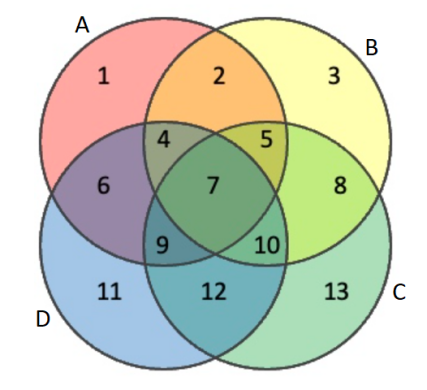
\includegraphics[width= 0.7\linewidth]{7}
%		\caption{\small\textit{\color{}}}
		\vspace*{-10pt}
	\end{figure}
	\textbf{\color{toancuabi}Bài $\pmb{5.}$} Bạn An di chuyển một que diêm từ chữ số $9$ hàng chục sang chữ số $1$ hàng nghìn và được số lớn nhất là:  
	\begin{figure}[H]
		\vspace*{-5pt}
		\centering
		\captionsetup{labelformat= empty, justification=centering}
		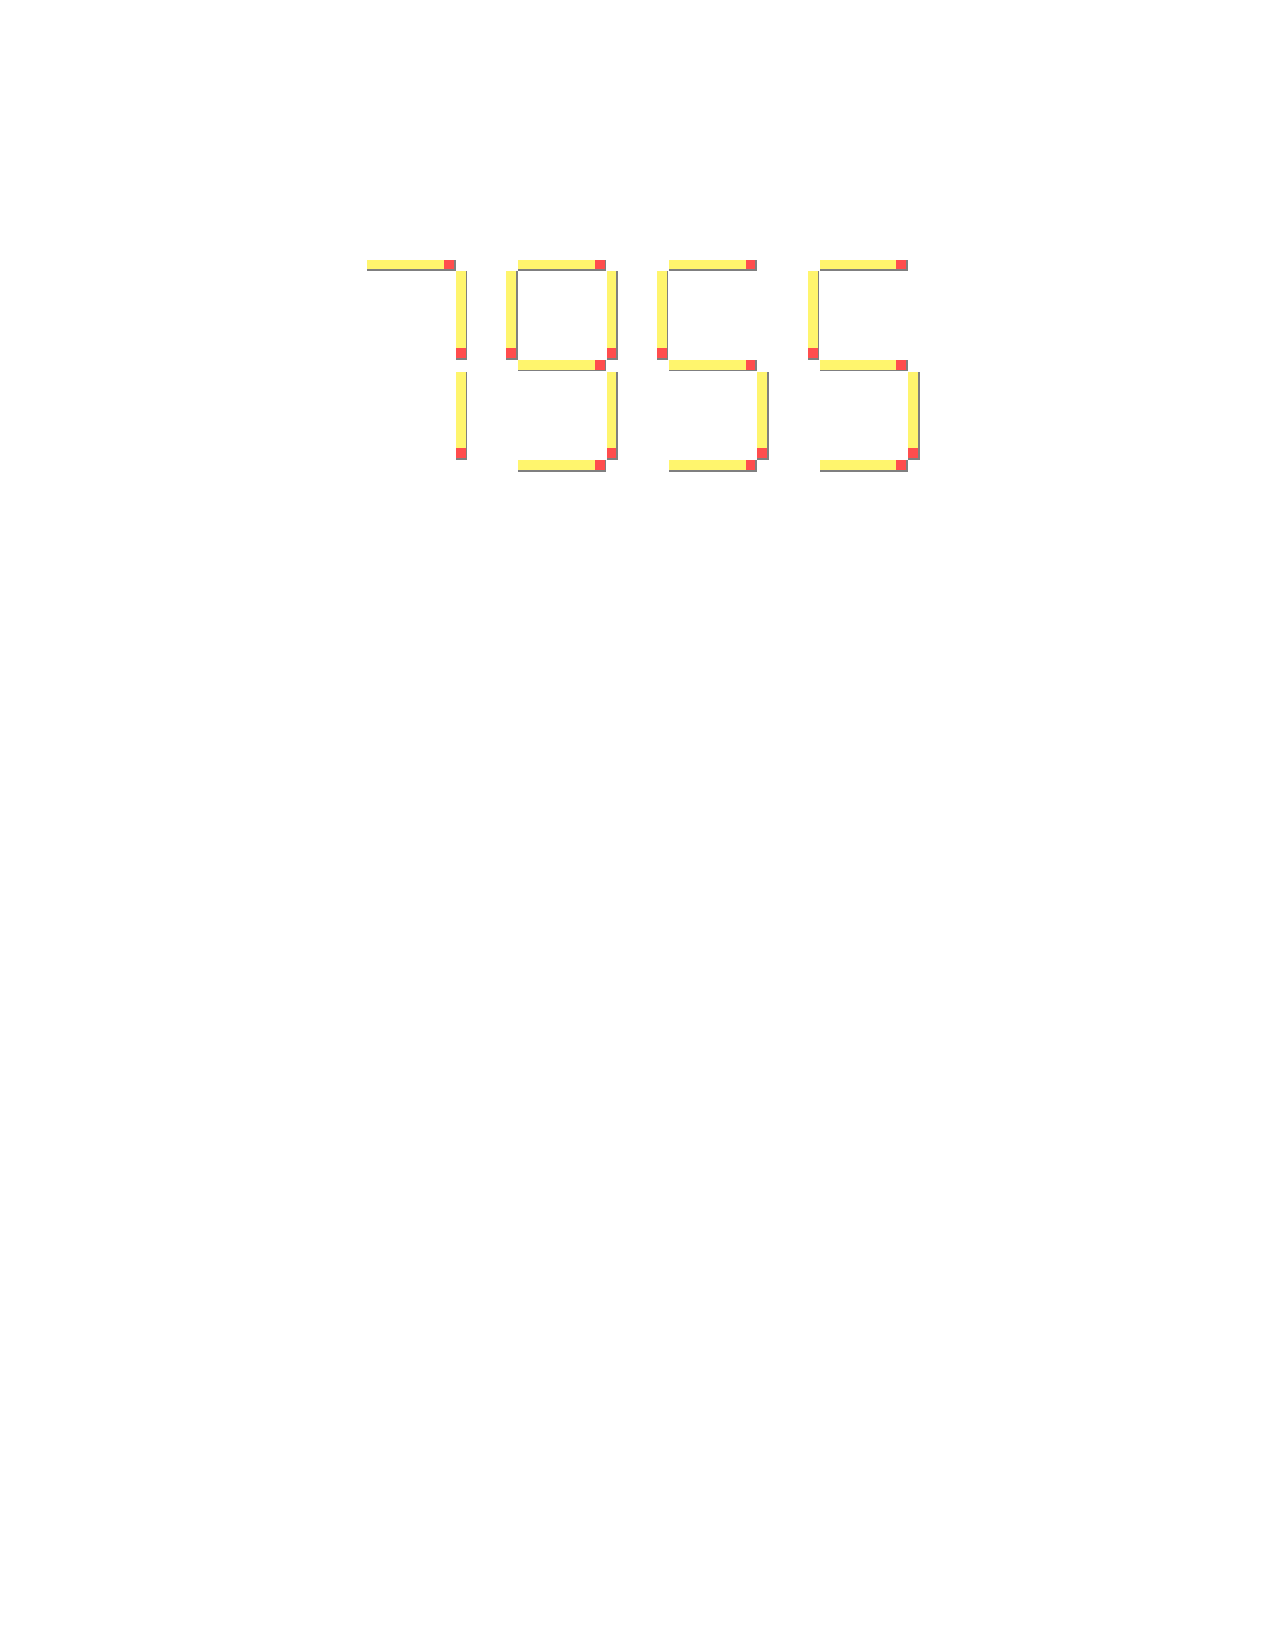
\includegraphics[width= 1\linewidth]{8}
%		\caption{\small\textit{\color{}}}
		\vspace*{-15pt}
	\end{figure}
	\textbf{\color{toancuabi}Bài $\pmb{6.}$} Ta vẽ đường thẳng như hình dưới đây, khi đó đường thẳng đi qua nhiều nhất $5$ ô vuông nhỏ.
	\begin{figure}[H]
		\vspace*{-5pt}
		\centering
		\captionsetup{labelformat= empty, justification=centering}
		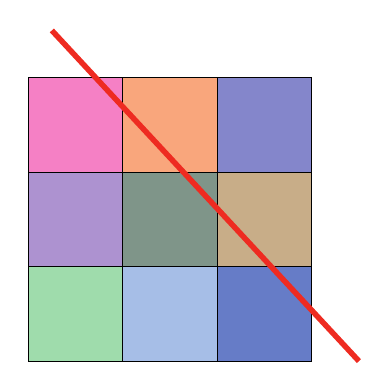
\begin{tikzpicture}[scale=1.2]
			\draw[fill=diendantoanhoc!50] (0,0) rectangle (1,1);
			\draw[fill=gocco!50] (0,1) rectangle (1,2);
			\draw[fill=toancuabi!50] (0,2) rectangle (1,3);
			\draw[fill=cackithi!50] (1,0) rectangle (2,1);
			\draw[fill=thachthuctoanhoc!50] (1,1) rectangle (2,2);
			\draw[fill=duongvaotoanhoc!50] (1,2) rectangle (2,3);
			\draw[fill=quantoan!80] (2,0) rectangle (3,1);
			\draw[fill=lichsutoanhoc!50] (2,1) rectangle (3,2);
			\draw[fill=timhieukhoahoc!60] (2,2) rectangle (3,3);
			\draw (0,0) grid (3,3);
			\draw[line width= 2pt, toanhocdoisong] (0.25,3.5) -- (3.5,0); 
		\end{tikzpicture}
%		\vspace*{-5pt}
	\end{figure}
	\textbf{\color{toancuabi}Bài $\pmb{7.}$} Tổng các cạnh của các hình tứ giác mà không phải là cạnh của ngôi sao lớn là:
	\begin{align*}
		7\times 5-3 = 32 \text{ (đơn vị).}
	\end{align*}
	Vậy chu vi của ngôi sao lớn ban đầu là:
	\begin{align*}
		18\times 5-32 = 58 \text{ (đơn vị).}
	\end{align*}
	\textbf{\color{toancuabi}Bài $\pmb{8.}$}  Đầu tiên bạn Châu đổi được $10:2=5$ (que kem). Với $5$ que kem mới này bạn đổi được $5:2=2$ que kem và dư $1$ vỏ que kem. Với $2$ vỏ que kem bạn Châu lại tiếp tục đổi được $1$ que kem. Cuối cùng $1$ vỏ que kem này và $1$ vỏ que kem còn thừa trước đó, bạn lại đổi được $1$ que kem nữa. Vậy tổng cộng bạn Châu được ăn số que kem là: 
	\begin{align*}
		10+5+2+1+1=19 \text{ (que kem).}
	\end{align*}
	\textbf{\color{toancuabi}Bài $\pmb{9.}$} Bằng cách ghép các phần được tô hồng như trong các minh họa dưới đây, ta thấy phần màu hồng gồm $4$ ô vuông nhỏ và phần màu trắng gồm $5$ ô vuông nhỏ cùng kích thước.
	\begin{figure}[H]
		\vspace*{-5pt}
		\centering
		\captionsetup{labelformat= empty, justification=centering}
		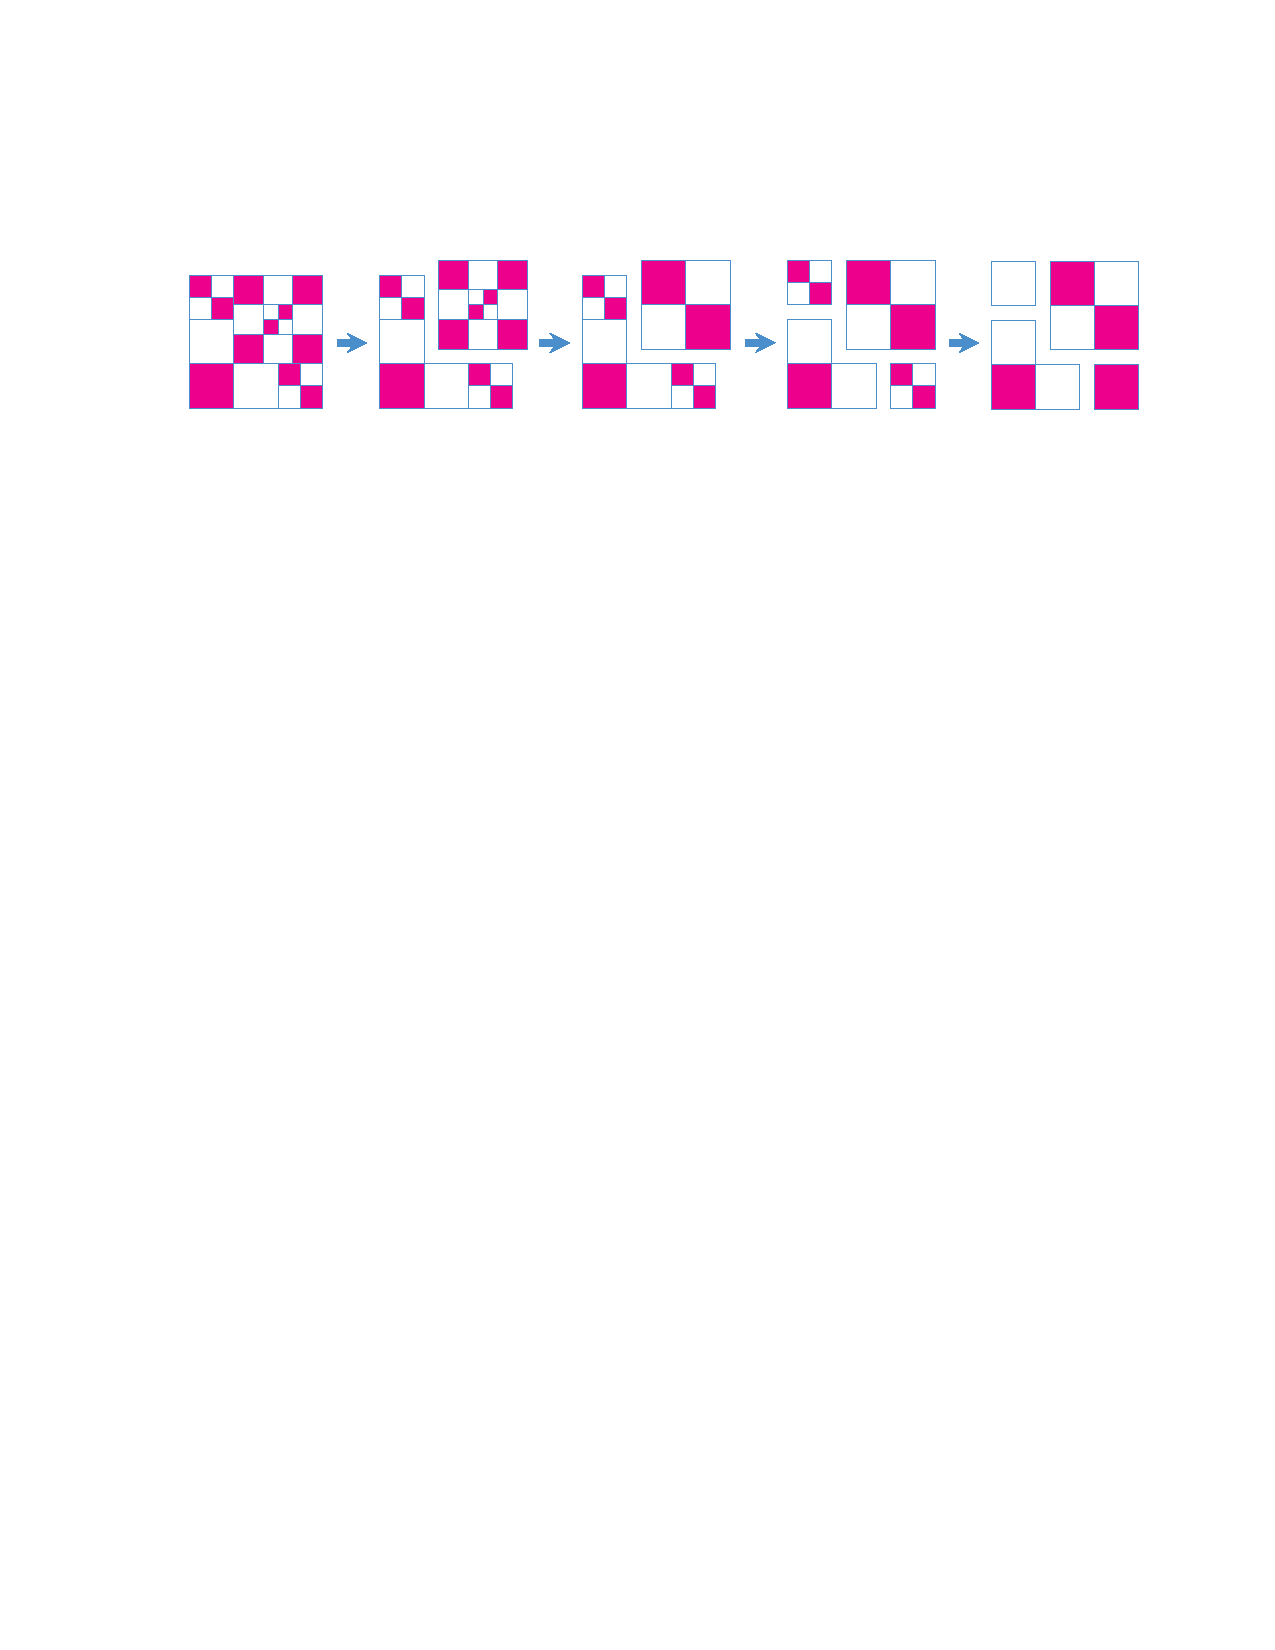
\includegraphics[width= 1\linewidth]{10a.pdf}
		%		\caption{\small\textit{\color{}}}
		\vspace*{-15pt}
	\end{figure}
	Như vậy diện tích một ô vuông nhỏ là: 
	\begin{align*}
		180:5 = 36 \text{ (đơn vị).}
	\end{align*}
	Do đó diện tích phần được tô hồng là: 
	\begin{align*}
		36\times 4 = 144 \text{ (đơn vị).}
	\end{align*}
	\textbf{\color{toancuabi}Bài $\pmb{10.}$} Vì hai bạn chung tiền mua thì vừa đủ $1$ cuốn tạp chí Pi, nên số tiền mà Nam còn thiếu chính là số tiền mà Dương có, số tiền mà Dương thiếu chính là số tiền mà Nam có. Vậy Dương có $12$ nghìn, Nam có $23$ nghìn. Vậy cuốn tạp chí Pi giá $12+23=35$ (nghìn).
\end{multicols}
\newpage
\graphicspath{{../toancuabi/pic/}}
\begingroup
\AddToShipoutPicture*{\put(106,650){
\includegraphics[scale=1]{../tieude.pdf}}}  
\centering
\endgroup
\vspace*{55pt} 
\begin{multicols}{2}
	Thám tử Xuân Phong đôi khi phải đột nhập vào những nơi hoang vắng, kỳ bí để tìm ra được dấu tích của những kẻ gây án. Một lần nọ, sau bao ngày cải trang để bám sát, theo dõi manh mối, thám tử biết tên trùm tội phạm đang trốn tránh trong một ngôi nhà hẻo lánh ở ngoại ô. Vừa đến trước cửa của ngôi nhà gỗ cổ kính, Xuân Phong gặp một bà lão với đôi mắt tinh anh nhìn mình với vẻ bí mật ``Thám tử đó phải không, tôi nhận ngay ra ngài, dù ngài đã cải trang rất kỹ. Phải chăng thám tử đang đi tìm tên trùm? Hắn đang ngồi dưới kia, trong căn phòng cùng những người trong hiệp hội Thương Gia, nhưng vô cùng nguy hiểm nếu ngài dùng vũ lực ở đây để bắt hắn. Tôi mách ngài nhé, ở dưới đó, có $10$ người, trong đó có lão trùm và những kẻ đồng phạm của lão. Bọn họ là những kẻ luôn nói dối, nhưng cũng có thể có cả những người lương thiện, luôn nói thật, ở ngay bên cạnh. Ngài hãy dùng trí thông minh của mình, chỉ được hỏi rất hạn chế câu hỏi để phán đoán ra những kẻ phạm tội là ai. Ngài hỏi nhiều câu hơn sẽ nguy hiểm cho cả những Thương gia lương thiện có thể có mặt ở đó. Và ngài hãy hứa với bà lão này sẽ đảm bảo an toàn cho tôi và gia đình, vì tôi đã liều mình thông báo tin mật này với Thám tử".
	\vskip 0.1cm
	Theo lời bà lão mách bảo, Xuân Phong lần theo một chiếc cầu thang cũ nát và đi xuống một căn phòng khuất dưới tầng hầm. Vừa mở cửa ra, thám tử đã thấy có $10$ người ăn mặc chỉnh tề như nhau, ngồi nghiêm trang quanh một chiếc bàn mười cạnh, mỗi người ngồi tại đỉnh của hình mười cạnh. Ánh sáng lờ mờ trong phòng đủ chiếu rõ dòng chữ ``Cuộc họp thường niên Hiệp hội Thương gia -- Khu vực Duyên Hải". Thật khó để xác định ai là kẻ nói dối trong số họ, vì vẻ ngoài họ đều giống như những Thương Gia thường gặp: quyền lực, sắc sảo và oai vệ.
	\begin{figure}[H]
		\centering
		\vspace*{-5pt}
		\captionsetup{labelformat= empty, justification=centering}
		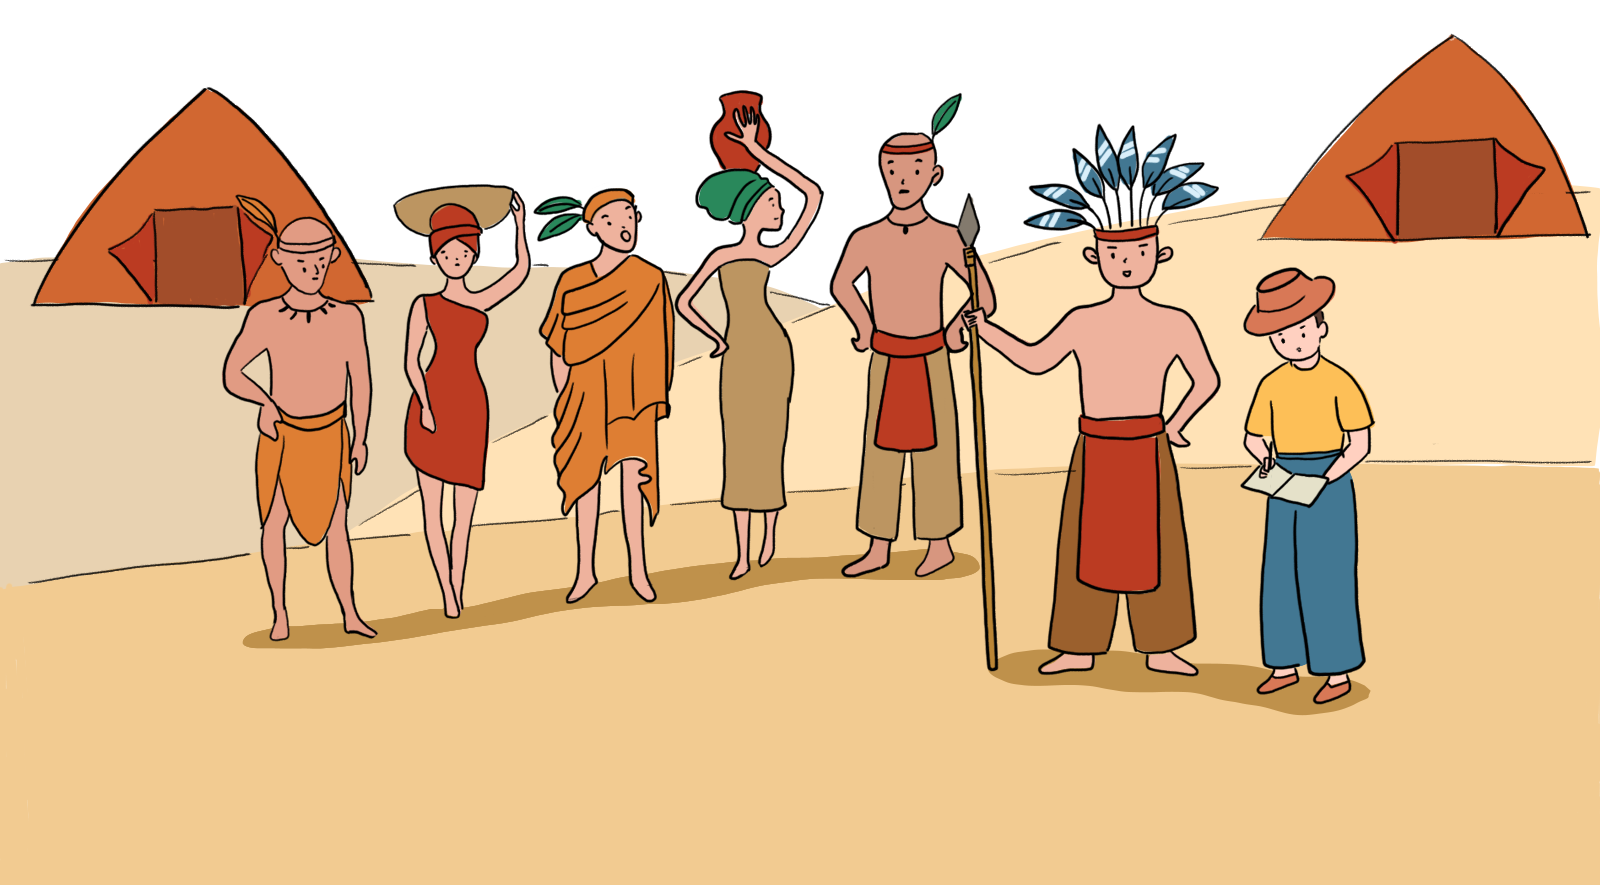
\includegraphics[width=1\linewidth]{xp}
		\vspace*{-15pt}
	\end{figure}
	Theo quy định của Hiệp hội Thương gia dành cho những người ngoài, qua lời của bà lão, Thám tử có thể đứng dậy bước tới một nơi bất kỳ nào đó trong căn phòng và chỉ được hỏi câu hỏi ``Khoảng cách từ chỗ tôi đứng đến người nói dối gần nhất trong số các anh là bao nhiêu?" cho tất cả những người trong phòng. Sau đó, mỗi người trong số $10$ người ngồi xung quanh bàn sẽ trả lời Thám tử, lúc này đã cải trang thành một Thương gia muốn gia nhập Hiệp hội. Thám tử không được phép đứng lên mặt bàn và tất cả mọi người, kể cả Thám tử, đều được phép dùng thước để đo khoảng cách tuỳ ý. Ta cũng được biết rằng ngoài $10$ người và Thám tử, trong phòng không còn có người lạ nào khác, hơn nữa $10$ người đều biết rõ ai trong số họ là nói thật và ai trong số họ là nói dối. Em hãy cho biết Xuân Phong có thể sử dụng ít nhất bao nhiêu câu hỏi như trên để biết chắc chắn ai trong số những người ngồi quanh bàn là nói~dối?
\end{multicols}
\newpage
\begingroup
\AddToShipoutPicture*{\put(115,670){\includegraphics[scale=1]{../tieude11.pdf}}} 
\centering
\endgroup
\vspace*{35pt}

\begin{multicols}{2}
	$\pmb{1.}$ Tuấn và Tú cùng tham gia một giải thi đấu cờ vua cùng các bạn học sinh khác trong trường. Hai bạn tổng cộng ghi được $6{.}5$ điểm, trong khi tất cả các bạn học sinh còn lại đều ghi được số điểm bằng nhau. Hỏi có tất cả bao nhiêu học sinh tham gia giải cờ vua đó? (Biết rằng trong giải thi đấu, mỗi người tham gia thi đấu đúng một ván với mỗi người còn lại, ghi được $1$ điểm sau mỗi trận thắng, $0{.}5$ điểm sau mỗi trận hoà và $0$ điểm sau mỗi trận thua).
	\begin{figure}[H]
		\centering
		\vspace*{-5pt}
		\captionsetup{labelformat= empty, justification=centering}
		\includegraphics[width=1\linewidth]{Hinh1}
		\vspace*{-20pt}
	\end{figure}
	$\pmb{2.}$ 	Lớp $6$A gồm $22$ bạn chia thành hai đội: Xanh gồm các bạn nam và Đỏ gồm các bạn nữ để tổ chức thi tài đối đáp, trả lời thông minh. Đầu tiên, bạn Hoa ở nhóm Đỏ đối đáp với $6$ bạn nam ở nhóm Xanh và giành chiến thắng. Tiếp theo, bạn Mai ở nhóm Đỏ đối đáp với $7$ bạn nam ở nhóm Xanh và cũng giành chiến thắng. Tiếp tục bạn Huệ ở nhóm Đỏ cũng chiến thắng $8$ bạn nam ở nhóm Xanh. Cứ tiếp tục như vậy, cuối cùng bạn Hà ở nhóm Đỏ đã đối đáp thông minh với toàn bộ các bạn nam ở nhóm Xanh và giành chiến thắng chung cuộc. Hỏi trong lớp có tất cả bao nhiêu bạn nam?
	\begin{figure}[H]
		\centering
		\vspace*{-5pt}
		\captionsetup{labelformat= empty, justification=centering}
		\includegraphics[width=1.01\linewidth]{Hinh2}
		\vspace*{-5pt}
	\end{figure}
	$\pmb{3.}$ 	Có bốn chủ doanh nghiệp tới thăm trường học cũ của mình, mang theo một số món quà với dự định sẽ trao tặng cho các học sinh đang học ở đó. Khi tất cả $252$ em học sinh được mời xếp thành một hàng ngang, chủ doanh nghiệp thứ nhất tặng quà cho mỗi em đứng thứ tư trong hàng (các em ở số thứ tự $4,8,12,$ \ldots). Chủ doanh nghiệp thứ hai lại tặng quà cho mỗi em đứng thứ bảy (các em ở số thứ tự $7,14,21$, \ldots). Chủ doanh nghiệp thứ ba trao tặng quà cho mỗi em đứng thứ mười một (các em ở số thứ tự $11,22,33$, \ldots). Chủ doanh nghiệp thứ tư sẽ tặng quà cho các em còn lại. Hỏi có bao nhiêu em học sinh nhận được quà từ mỗi chủ doanh nghiệp?
	\begin{figure}[H]
		\centering
		\vspace*{-5pt}
		\captionsetup{labelformat= empty, justification=centering}
		\includegraphics[width=1\linewidth]{Hinh3}
		\vspace*{-15pt}
	\end{figure}
	$\pmb{4.}$ 	Có ba nhà tài trợ quyết định giúp đỡ một tạp chí khoa học thường thức với tên gọi là Phi. Nhà tài trợ Quốc trao tặng một khoản tiền tính bằng dollar gồm có $4$ chữ số: $2$ chữ số đứng trước dấu phẩy, và hai chữ số sau dấu phẩy, trong đó số cent lẻ (tức là hai chữ số đứng sau dấu phẩy) bằng với đúng số dollar chẵn (tức là hai chữ số đứng trước dấu phẩy; ta nhớ lại $100$ cent $= 1$ dollar). Nhà tài trợ Minh tặng số tiền với số dollar chẵn lớn hơn $3$ dollar so với số dollar chẵn mà nhà tài trợ Quốc đã tặng nhưng số cent lẻ lại ít hơn $8$ lần số cent lẻ của nhà tài trợ Quốc. Nhà tài trợ Vũ hào phóng đem tặng số tiền bằng $1/7$ tổng số tiền của hai nhà tài trợ Quốc và Minh đã trao cộng lại. Hỏi số tiền ủng hộ của ba nhà tài trợ cho tạp chí Phi là bao nhiêu?
	\begin{figure}[H]
		\centering
%		\vspace*{-5pt}
		\captionsetup{labelformat= empty, justification=centering}
		\includegraphics[width=0.8\linewidth]{Hinh4}
		\vspace*{-10pt}
	\end{figure}
	\vskip 0.1cm
	$\pmb{5.}$ 	Trên hòn đảo Ngọc ở giữa một đại dương xanh ngắt có $100$ thổ dân sinh sống, một số người trong họ luôn nói dối, còn những người còn lại luôn nói thật. Mỗi một thổ dân thờ phụng đúng một trong ba vị thần: thần Mặt trời, thần Mặt trăng hoặc thần Đất. Người ta hỏi mỗi thổ dân ba câu hỏi sau đây:
	\begin{figure}[H]
		\centering
		\vspace*{-5pt}
		\captionsetup{labelformat= empty, justification=centering}
		\includegraphics[width=1\linewidth]{Hinh5}
		\vspace*{-20pt}
	\end{figure}
	$1.$ Ông (bà) có thờ phụng thần Mặt trời hay không?
	\vskip 0.1cm
	$2.$ Ông (bà) có thờ phụng thần Mặt trăng hay không?
	\vskip 0.1cm
	$3.$ Ông (bà) có thờ phụng thần Đất hay không?
	\vskip 0.1cm
	Có $60$ người trả lời khẳng định ``có" với câu hỏi thứ nhất, $40$ người trả lời khẳng định ``có" với câu hỏi thứ hai và $30$ người trả lời khẳng định ``có" với câu hỏi thứ ba. Hỏi trên đảo Ngọc có bao nhiêu thổ dân nói dối?
	\vskip 0.1cm
	$\pmb{6.}$ 	Có $100$ em học sinh được mời tới buổi tổng kết cuối năm học của nhà trường. Các ghế trong phòng họp được xếp ngay ngắn thẳng hàng theo dạng một hình vuông với $10$ dãy ghế, mỗi dãy có đúng $10$ chiếc ghế. Buổi họp phải diễn ra muộn hơn do bị cắt điện, vì thế các em học sinh bắt đầu bàn luận trao đổi với các bạn bên cạnh về kết quả điểm trung bình của mình. Em học sinh nào thấy trong tất cả những bạn ngồi kề sát mình: bên trái, bên phải, đằng sau, đằng trước và theo các đường chéo, chỉ có tối đa một bạn có điểm trung bình cao hơn hoặc bằng điểm trung bình của  mình, sẽ tự coi mình là ``có thành tích".
	\begin{figure}[H]
		\centering
		\vspace*{-10pt}
		\captionsetup{labelformat= empty, justification=centering}
		\includegraphics[width=0.85\linewidth]{Hinh6}
		\vspace*{-10pt}
	\end{figure}
	Hỏi trong buổi họp đó có thể có tối đa bao nhiêu em học sinh đã tự coi mình là ``có thành tích" trong học tập?
\end{multicols}
\vspace*{-10pt}
{\color{toancuabi}\rule{1\linewidth}{0.1pt}}
\begingroup
\AddToShipoutPicture*{\put(114,178){\includegraphics[scale=1]{../tieude2.pdf}}} 
\centering
\endgroup
\vspace*{75pt}

\begin{multicols}{2}
	$\pmb{1.}$ Các bạn nam mang kẹo tới lớp để tặng cho các bạn nữ. Bạn Phúc nói rằng mình đã mang tới đúng một nửa tổng số kẹo. Bạn Kiên nói rằng mình đã mang tới đúng một phần ba tổng số kẹo và chỉ chia kẹo của mình cho Mai và Tuyết, hơn nữa Mai được nhiều hơn so với Tuyết là $3$ chiếc kẹo. Em hãy chứng tỏ rằng có một bạn trong số Phúc và Kiên đã \linebreak nhầm lẫn.\\
	\textit{Lời giải.} Giả sử cả hai bạn Phúc và Kiên đều không nhầm lẫn. Do Phúc không nhầm, nên tổng số kẹo được mang tới lớp phải là số chẵn (gấp $2$ lần số kẹo mà Phúc mang tới). Do Kiên cũng mang tới một số kẹo là số nguyên, bằng $1/3$ của một số chẵn, nên Kiên cũng mang tới một số kẹo là số chẵn. Theo lời của Kiên, số kẹo mà cậu đã tặng cho các bạn nữ là một số lẻ, do số kẹo mà Mai và Tuyết nhận được khác tính chẵn lẻ (hơn kém nhau là $3$ chiếc, mà $3$ là một số lẻ), mà tổng của hai số khác tính chẵn lẻ là một số lẻ. Ta nhận được mâu thuẫn. Suy ra có ít nhất một bạn nam trong số Phúc và Kiên đã nhầm lẫn.
	\begin{figure}[H]
			\centering
		\vspace*{-5pt}
		\captionsetup{labelformat= empty, justification=centering}
		\includegraphics[width=0.6\linewidth]{Pi7_bai1}
		\vspace*{-10pt}
	\end{figure}
	$\pmb{2.}$ Ba người thợ cùng đào một chiếc hố. Họ luân phiên lần lượt làm việc, mỗi người làm việc trong một thời gian nhất định. Nếu trong khi một người làm việc hai người còn lại cũng đồng thời đào hố thì hai người này sẽ đào được đúng một nửa hố. Hỏi nếu cả ba người cùng đồng thời đào thì họ sẽ làm nhanh hơn được bao nhiêu lần so với cách làm luân phiên ban đầu?
	\begin{figure}[H]
		\centering
		\vspace*{-5pt}
		\captionsetup{labelformat= empty, justification=centering}
		\includegraphics[width=1\linewidth]{Pi7_bai2}
		\vspace*{-20pt}
	\end{figure}
	\textit{Lời giải.} 	Giả sử trong thời gian mỗi người đào ở chiếc hố ban đầu, hai người còn lại sẽ đi đào một chiếc hố bổ sung thêm khác. Như vậy khi kết thúc công việc, cùng với chiếc hố ban đầu, họ sẽ đào thêm được $3\cdot 0{.}5 = 1{.}5$ chiếc hố. Do đó, nếu cả ba người cùng làm công việc đào, thì trong cùng số thời gian như ban đầu, họ sẽ đào được $1+1{.}5=2{.}5$ (hố). Vậy, nếu cả ba người cùng đào thì họ sẽ làm nhanh hơn được $2{.}5$ lần so với cách đào luân phiên lần lượt như ban đầu.
	\vskip 0.1cm
	$\pmb{3.}$ Ba bạn Gấu, Thỏ và Mèo cùng quyết định xây một con đường từ nhà tới bờ suối với chiều dài $160m$. Các bạn thoả thuận sẽ đầu tư cho dự án mở đường quan trọng này với công sức đều như nhau. Cuối cùng khi dự án hoàn thành, hoá ra bạn Thỏ đã xây được $60$ mét đường, bạn Mèo xây được $100$ mét đường, còn bạn Gấu mải ngủ đông nên không xây được mét nào. Tuy nhiên, Gấu mang tới đóng góp bằng tiền cho dự án là $16$ triệu đồng từ số mật ong bán được của mình. Hỏi hai bạn Mèo và bạn Thỏ cần phải phân chia số tiền cho nhau như thế nào?
	\begin{figure}[H]
		\centering
		\vspace*{-5pt}
		\captionsetup{labelformat= empty, justification=centering}
		\includegraphics[width=1\linewidth]{Pi7_bai3}
		\vspace*{-15pt}
	\end{figure}
	\textit{Lời giải.} 	Mỗi bạn theo kế hoạch phải xây đúng $\dfrac{160}{3} = 53\dfrac{1}{3}$  mét đường. Thỏ xây được $60$ (m) và Gấu xây được $100$ (m). Như vậy bạn Thỏ đã xây thay cho bạn Gấu số mét đường là
	\begin{align*}
		60 - 53 \frac{1}{3} = 6 \frac{2}{3}= \frac{20}{3} \text{ (m)},
	\end{align*}
	còn bạn Mèo đã xây thay cho bạn Gấu số mét đường
	\begin{align*}
		100- 53 \frac{1}{3} = 46 \frac{2}{3}=\frac{140}{3} \text{ (m).}
	\end{align*}
	Vì vậy số tiền mà bạn Gấu mang tới phải chia cho Thỏ và Mèo theo tỷ lệ $2: 14$, tức là Mèo được $14$ triệu đồng, còn Thỏ được $2$ triệu đồng từ số tiền đóng góp công sức của Gấu.
	\vskip 0.1cm
	$\pmb{4.}$ Bé Ly phải đi trồng hoa vào một hàng các chậu rất dài đặt thành hàng dọc ở công viên. Bé được giao nhiệm vụ là phải trồng hai loại hoa khác nhau vào hai chiếc chậu nếu giữa hai chậu này có đúng hai chiếc chậu, hoặc đúng ba chiếc chậu, hoặc đúng năm chiếc chậu khác. Hỏi bé Ly phải cần ít nhất bao nhiêu loại hoa để thực hiện được nhiệm vụ?
	\begin{figure}[H]
		\centering
		\vspace*{-5pt}
		\captionsetup{labelformat= empty, justification=centering}
		\includegraphics[width=0.45\linewidth]{Pi7_bai4}
		\vspace*{-10pt}
	\end{figure}
	\textit{Lời giải.} Trước tiên ta thấy rằng bé Ly có thể chỉ cần $3$ loại hoa là thực hiện được nhiệm vụ. Thật vậy, giả sử Ly có $3$ loại là $A, B, C$. Khi đó nếu Ly trồng $3$ chậu đầu tiên trong hàng bằng loại $A$, $3$ chậu tiếp theo bằng loại $B$, $3$ chậu tiếp loại $C$ và lại $3$ chậu tiếp theo quay lại bằng loại $A$, vv \ldots thì rõ ràng yêu cầu đặt ra được thực hiện. 
	\vskip 0.1cm
	Bây giờ giả sử Ly chỉ có $2$ loại hoa là $A$ và $B$. Nếu Ly trồng ở chậu thứ nhất bằng hoa loại $A$ (không mất tính tổng quát), suy ra các chậu có số thứ tự tiếp theo là $4, 5, 7$ phải được trồng bằng hoa loại $B$. Nhưng khi đó giữa hai chậu số $4$ và số $7$ đều được trồng cùng loại hoa $B$ nhưng giữa chúng có đúng hai chậu khác là số $5$ và số $6$, suy ra mâu thuẫn với yêu cầu.
	\vskip 0.1cm
	Vậy Ly cần ít nhất $3$ loại hoa để trồng theo yêu cầu đặt ra.
	 \vskip 0.1cm
	$\pmb{5.}$ Trước một trận bóng đá giữa hai đội Xóm Đông và Xóm Bắc có $5$ dự đoán kết quả được đưa ra:
	\vskip 0.1cm
	$a)$	Sẽ không có tỷ số hoà;
	\vskip 0.1cm
	$b)$	Đội Xóm Đông sẽ bị thủng lưới;
	\vskip 0.1cm
	$c)$	Đội Xóm Bắc sẽ thắng;
	\vskip 0.1cm
	$d)$	Đội Xóm Bắc sẽ không thua;
	\vskip 0.1cm
	$e)$	Trong trận bóng sẽ có đúng $3$ bàn thắng được ghi.
	\vskip 0.1cm
	Sau khi trận bóng kết thúc, hoá ra chỉ có đúng $3$ dự đoán là chính xác. Vậy trận đấu đã kết thúc với tỷ số như thế nào?
	\begin{figure}[H]
		\centering
%		\vspace*{-5pt}
		\captionsetup{labelformat= empty, justification=centering}
		\includegraphics[width=0.85\linewidth]{Pi7_bai5}
		\vspace*{-10pt}
	\end{figure}
	\textit{Lời giải.} Giả sử là đội Xóm Bắc thắng. Khi đó $4$ dự đoán $a)$, $b)$ $c)$ và $d)$ đều đúng, mâu thuẫn với điều kiện đặt ra.
	\vskip 0.1cm
	Tiếp theo, giả sử trận đấu kết thúc với tỷ số hoà. Khi đó ta lại có các dự đoán $a)$, $c)$ và $e)$ đều sai, điều này cũng mâu thuẫn với điều kiện đã cho.
	\vskip 0.1cm
	Vì vậy, trong trận bóng này đội Xóm Bắc đã thua. Khi đó các dự đoán $c)$ và $d)$ đều sai, và $3$ dự đoán còn lại là đúng. Có nghĩa là: trận đấu không có tỷ số hoà, có ít nhất một trái bóng được đưa vào lưới của đội Xóm Đông, và trong trận bóng có đúng $3$ bàn thắng được ghi. Điều đó có nghĩa là trận bóng kết thúc với tỷ số $1:2$ nghiêng về phía đội Xóm Đông.
	\vskip 0.1cm
	$\pmb{6.}$ 	Tại trại hè có $20$ em học sinh tham gia trò chơi Điệp viên tí hon diễn ra trong $2$ tuần. Mỗi Điệp viên tí hon sẽ theo dõi và viết báo cáo tỉ mỉ về sở thích cá nhân của $10$ em khác trong số $20$ em này để nộp cho Sở chỉ huy. Em hãy chứng tỏ rằng có ít nhất $10$ cặp Điệp viên tí hon đã theo dõi lẫn nhau và viết báo cáo về nhau.
	\begin{figure}[H]
		\centering
		\vspace*{-5pt}
		\captionsetup{labelformat= empty, justification=centering}
		\includegraphics[width=0.75\linewidth]{Pi7_bai6}
		\vspace*{-15pt}
	\end{figure}
	\textit{Lời giải.} Số các cặp Điệp viên tí hon là $\dfrac{20\times 19}{2} = 190$ (cặp). Có tất cả $10\times 20=200$ báo cáo được gửi về Sở chỉ huy vào cuối đợt chơi, suy ra phải có ít nhất $10$ cặp Điệp viên mà hai người trong mỗi cặp báo cáo lẫn nhau về Sở chỉ huy.
\end{multicols}

\newpage
\begingroup
\thispagestyle{toancuabinone}
\blfootnote{$^1$\color{toancuabi}Ottawa, Canada.}
\AddToShipoutPicture*{\put(60,733){\includegraphics[width=17.2cm]{../mathc.pdf}}}
%\AddToShipoutPicture*{\put(-2,733){\includegraphics[width=17.2cm]{../mathl.pdf}}} 
\AddToShipoutPicture*{\put(110,675){\includegraphics[scale=1]{../tieudeb.pdf}}} 
\centering
\endgroup
\vspace*{35pt}

\begin{multicols}{2}
	In this article, we discuss the Extremal Principle and its applications.
	One of the simplest forms of the principle is as follow:
	``in a finite set of numbers, there is a number with minimal value,
	i.e. it is smaller than or equal to any other number in the set.
	Similarly there is a number with maximal value,
	i.e. it is larger than or equal to any other number in the set."
	\vskip 0.1cm
	\textit{Proof by contradiction} is an extremely useful tool when combining with the Extremal Principle,
	as you will see in below examples.
	\vskip 0.2cm
	\PIbox{{\color{toancuabi}\textbf{\color{toancuabi}Example} (Dancing at a party)}
			At a party no boy danced with all the girls,
			but each girl dances with at least one boy.
			Prove that there are two pairs of girl--boy $(g_1, b_1)$ and $(g_2, b_2)$
			who danced with each other but $g_1$ did not dance with $b_2$
			and $g_2$ did not dance with $b_1.$}
	\vskip 0.2cm
	\textit{Solution.}
		Let $b_1$ be \textit{the boy who danced with the maximum number of girls.}
		Then there is a girl $g_2$ who he did not danced with.
		For $g_2$ there is a boy $b_2$ that $(g_2,b_2)$ danced together.
		Among the girls who danced with $b_1$ there is at least one $g_1$ who did not danced with $b_2,$
		otherwise $b_2$ danced with $g_2$ and all the girls that $b_1$ danced with,
		meaning $b_2$ danced with more girls than $b_1,$ contradicting with the choice of $b_1.$
	\vskip 0.2cm
	\PIbox{{\color{toancuabi}\textbf{\color{toancuabi}Example} (Infinity by contradiction)}
			$\Omega$ is a set of points on the plane.
			Every point in $\Omega$ is a midpoint of two points in $\Omega$.
			Show that $\Omega$ is infinite set.}
	\vskip 0.2cm
	\textit{Solution.}
	Suppose that $\Omega$ is a finite set.
	According to the Extremal Principle,
	\textit{there exists two points $A, B \in \Omega,$ such that the distance $AB$ is maximal.}
	\vskip 0.1cm
	Now, since $B \in \Omega,$ there exist two points $C,D \in \Omega$ so that $B$ is the midpoint of $CD.$
	\begin{figure}[H]
			\vspace*{-5pt}
			\centering
			\captionsetup{labelformat= empty, justification=centering}
			\begin{tikzpicture}[toancuabi,scale=0.75]
					\draw  (0.,0.)-- (3.,3.);
					\draw  (3.,3.)-- (5.,-3.);
					\draw  (5.,-3.)-- (0.,0.);
					\draw  (0.,0.)-- (4.,0.);
						\draw [fill=white] (0.,0.) circle (1.5pt);
						\draw (-0.32,0.11) node {$A$};
						\draw [fill=white] (3.,3.) circle (1.5pt);
						\draw (3.14,3.37) node {$C$};
						\draw [fill=white] (5.,-3.) circle (1.5pt);
						\draw (5.32,-3.01) node {$D$};
						\draw [fill=white] (4.,0.) circle (1.5pt);
						\draw (4.36,0.15) node {$B$};
				\end{tikzpicture}
			\vspace*{-10pt}
		\end{figure}    
	Since one of the angles $\angle ABC,$ $\angle ABD,$ says $\angle ABD$ is at least $90^{\circ},$
	thus in $\triangle ABD,$ $AD > AB.$
	This contradicts the assumption that $A, B$ are the two points in $\Omega,$ such that the distance $AB$ is maximal.
	\vskip 0.1cm	
	Thus, there are no such two points $A, B,$ so $\Omega$ is infinite set.
	\vskip 0.2cm
	\PIbox{{\color{toancuabi}\textbf{\color{toancuabi}Example} (How many olives did the knights eat?)}
		At the dinner of King Anthony, several knights sits around a round table eating green olives.
		Minh, the Magician, made sure that each knight ate either twice as many olives
		or $10$ olives less than his right neighbour. 
		Is that possible that the knights could have eaten exactly $1001$ olives?}
	\vskip 0.2cm
	\textit{Solution.}
	Let assume that the knights have eaten exactly $1001$ olives.
	Let choose the knight who \textit{ate the smallest number of olives}.
	(If there are some of them, choose one.)
	His neighbour on the left, knight $k$, ate either $10$ less or twice more.
	Since the knight we chose ate the smallest number of olives, then knight $k$ ate twice as many.
	Therefore, knight $k$ ate an even number of olives. 
	\vskip 0.1cm	
	The neighbour on the left of knight $k$ ate either twice as many olives or $10$ olives less,
	hence he ate an even number of olives as well. Making the full circle, we'll end us with the first knight,
	who must have eaten an even number of olives as well.
	\vskip 0.1cm	
	Therefore, the total number of olives must be an even number.
	The number of olives eaten cannot be $1001.$
	\vskip 0.2cm
	\PIbox{{\color{toancuabi}\textbf{\color{toancuabi}Example} (Chop the flies)}
		$25$ flies are resting on the outdoor table in the garden, waiting for lunch to be served.
		It is known that for any three of them, two are at a distance less than $20$ cm;
		and there are at least a pair of flies that are further than $20$ cm from each other.
		\vskip 0.1cm
		Minh's mother gave him a fly swatter, shown below, with a hoop of radius $20$ cm,
		With a single strike he can swat the flies where the hoop landed.
		In \textit{at least} how many strikes can he swat all of them?
		\textit{Note that Minh is so fast that the flies do not have time for reaction during and between his lightning strikes.}}
	\vskip 0.2cm
	\textit{Solution.}
	If no $2$ flies are further than $20$ cm from each other,
	Minh can strike them all in $1$ strike by aiming the center of the swatter at any fly. 
	But this is not the case, so let’s assume there are $2$ flies, $A$ and $B$, that are more than $20$ cm apart.
	Then, every other fly is either in a $20$ cm radius of $A$ or in a $20$ cm radius of $B.$
	Out of the $23$ remaining flies either at least $12$ will be in the $20$ cm radius of $A$
	or $12$ will be in the $20$ cm radius of $B$.
	Swatting that the $A$ or $B$ fly with the center of the swatter kills at least $13$.
	\vskip 0.1cm
	Thus, by $2$ strikes, he can swat them all.
\end{multicols}

%	\newpage 
%	
%	\setcounter{figure}{0}
%	\thispagestyle{thachthuctoanhocnone}
\pagestyle{thachthuctoanhoc}
\everymath{\color{thachthuctoanhoc}}
\graphicspath{{../thachthuctoanhoc/pic/}}
\begingroup
\AddToShipoutPicture*{\put(0,616){\includegraphics[width=19.3cm]{../thachthuctoanhoc/bannerthachthuc}}}
\centering
\vspace*{4cm}
\endgroup
\vspace*{-8pt}
\begin{tBox}
	\begin{itemize}[leftmargin = 13pt, itemsep = 1.0pt] 
		\item Mỗi bài toán đề xuất (kèm theo lời giải) cần được nêu rõ là bài sáng tác hay bài sưu tầm.
		%		\item Mỗi bài toán đề xuất (kèm theo lời giải) cần được nêu rõ là bài sáng tác hay bài sưu tầm (nếu là bài sưu tầm, cần ghi rõ nguồn).
		\item Bài giải cho mỗi bài toán cần được trình bày trong một file riêng hoặc
		một tờ giấy riêng.
		\item  Người đề xuất bài toán hoặc gửi bài giải cho các bài toán trong mục ``Thách thức kỳ này" cần ghi rõ họ, đệm, tên và nơi làm việc/học tập, số điện thoại liên hệ. Nếu là học sinh (hoặc sinh viên) cần ghi rõ là học sinh lớp mấy (hoặc sinh viên năm thứ mấy).
		\item Các bài toán trong mục Thách thức kỳ này hướng tới các độc giả là học sinh phổ thông; được phân chia thành các mức độ $B$, $A$, và được sắp xếp theo độ khó tăng dần, theo đánh giá chủ quan của Ban biên tập. Các bài toán mức độ $B$ không đòi hỏi các kiến thức vượt quá chương trình môn Toán cấp THCS; các bài toán mức độ $A$ không đòi hỏi các kiến thức vượt quá chương trình môn Toán cấp THPT.
		\item Cách thức gửi bài toán đề xuất hoặc lời giải: gửi file thu được bằng cách scan, ảnh chụp (rõ nét) của bản viết tay, hoặc được soạn thảo bằng các phần mềm Latex, Word tới \url{bbt@pi.edu.vn} hoặc gửi qua đường bưu điện tới Tòa soạn (xem địa chỉ tại bìa $2$).
		\item Hạn gửi lời giải cho các bài toán P$751$--P$760$: trước ngày $15/12/2023$.
	\end{itemize}
\end{tBox}
\begin{center}
	\vspace*{-5pt}
	\textbf{\color{thachthuctoanhoc}\color{thachthuctoanhoc}\color{thachthuctoanhoc}\color{thachthuctoanhoc}\color{thachthuctoanhoc}THÁCH THỨC KỲ NÀY}
	\vspace*{-5pt}
\end{center}
\begin{multicols}{2}
	\setlength{\abovedisplayskip}{4pt}
	\setlength{\belowdisplayskip}{4pt}
	{\color{thachthuctoanhoc}{\usefont{T5}{qag}{b}{n} P751.}}
	(Mức $B$) Người ta ghép khít năm hình chữ nhật bằng nhau với nhau, để được một hình dài $27$cm và rộng $15 $cm, như ở hình vẽ dưới đây. Biết rằng, đoạn thẳng $A C$ chia hình đó thành hai phần có diện tích bằng nhau. Hãy tính độ dài đoạn thẳng $A B$.
	\begin{figure}[H]
		\vspace*{-10pt}
		\centering
		\captionsetup{labelformat= empty, justification=centering}
		\definecolor{qqqqff}{rgb}{0,0,1}
		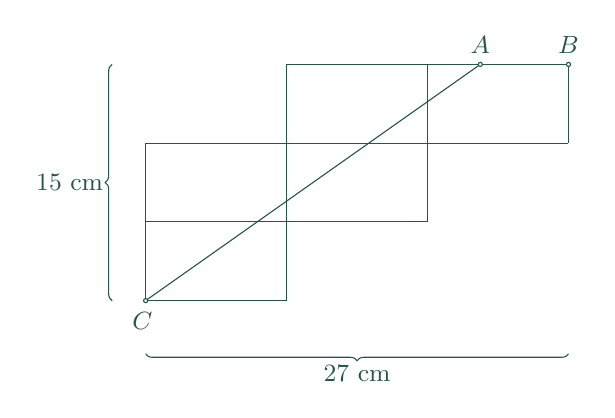
\begin{tikzpicture}[scale=0.5,thachthuctoanhoc, node font=\small]
			\draw  (-4,2)-- (-4,-2);
			\draw  (-4,-2)-- (-0.42,-2);
			\draw  (-0.42,-2)-- (-0.42,4);
			\draw  (-4,2)-- (6.74,2);
			\draw  (6.74,2)-- (6.74,4);
			\draw  (6.74,4)-- (-0.42,4);
			\draw  (3.16,4)-- (3.16,0);
			\draw  (3.16,0)-- (-4,0);
			\draw  (-4,-2)-- (4.5,4);
			\draw[decoration={brace,mirror,raise=5pt},decorate]
			(-4,-3) -- node[below = 6pt] {$27\text{ cm}$} (6.74,-3);
			\draw[decoration={brace,mirror,raise=5pt},decorate]
			(-4.5,4) -- node[left = 5pt] {$15\text{ cm}$} (-4.5,-2);
			\draw [fill=white] (-4,-2) circle (1.5pt);
			\draw (-4.08,-2.52) node {$C$};
			\draw [fill=white] (6.74,4) circle (1.5pt);
			\draw (6.74,4.5) node {$B$};
			\draw [fill=white] (4.5,4) circle (1.5pt);
			\draw (4.5,4.5) node {$A$};
		\end{tikzpicture}
		\vspace*{-10pt}
	\end{figure}
	\begin{flushright}
		\textit{Đăng Hải, Hà Nội (st)}
	\end{flushright}
	{\color{thachthuctoanhoc}{\usefont{T5}{qag}{b}{n} P752.}}
	(Mức $B$) Cho $x,y,z$ là các số thực thoả mãn $x^2y+y^2z+z^2x=1$ và $xy^2+yz^2+zx^2=2$. Tính giá trị biểu thức
	\begin{align*}
		P=\left(\!x^2\!+\!xy\!+\!y^2\!\right)\!\left(\!y^2\!+\!yz\!+\!z^2\!\right)\!\left(\!z^2\!+\!zx\!+\!x^2\!\right).
	\end{align*}
	\begin{flushright}
		\textit{Trần Quốc Luật, Tp. Hồ Chí Minh}
	\end{flushright}
	{\color{thachthuctoanhoc}{\usefont{T5}{qag}{b}{n} P753.}}
	(Mức $B$) Cho đường tròn $(O)$ với đường kính $AB = 2R$. Gọi $C$ là trung điểm của $OA$. $M$ là một điểm nằm trên $(O)$. Đường thẳng $MC$ cắt $(O)$ tại điểm thứ hai $D$.  Đường thẳng qua $D$ và vuông góc với $AB$, cắt $(O)$ tại điểm thứ hai $E$. Đường thẳng $ME$ cắt đường thẳng $AB$ tại điểm $F$. Tìm vị trí của điểm $M$  sao cho tổng $EF + MC$ có giá trị nhỏ nhất.
	\begin{figure}[H]
%		\vspace*{5pt}
		\centering
		\captionsetup{labelformat= empty, justification=centering}
		\definecolor{qqwuqq}{rgb}{0.,0.39215686274509803,0.}
		\definecolor{uuuuuu}{rgb}{0.26666666666666666,0.26666666666666666,0.26666666666666666}
		\definecolor{xdxdff}{rgb}{0.49019607843137253,0.49019607843137253,1.}
		\definecolor{ududff}{rgb}{0.30196078431372547,0.30196078431372547,1.}
		\begin{tikzpicture}[thachthuctoanhoc]
			\draw[color=qqwuqq,fill=qqwuqq,fill opacity=0.10000000149011612] (-1.5617418181909823,1.) -- (-1.5617418181909823,1.1880461622337974) -- (-1.7497879804247796,1.1880461622337974) -- (-1.7497879804247796,1.) -- cycle; 
			\draw  (0.,1.) circle (2.cm);
			\draw  (-2.,1.)-- (2.,1.);
			\draw  (-4.,1.)-- (0.4991521613769648,2.936710386142622);
			\draw  (0.4991521613769648,2.936710386142622)-- (-1.7497879804247796,0.03137105991975908);
			\draw  (-2.,1.)-- (-4.,1.);
			\draw  (-1.7497879804247796,1.968628940080241)-- (-1.7497879804247796,0.03137105991975908);
				\draw [fill=white] (0.,1.) circle (1.5pt);
				\draw (0.09082211690268885,1.2491318135923188) node {$O$};
				\draw [fill=white] (-2.,1.) circle (1.5pt);
				\draw (-2.2228335500515635,0.7335225357666101) node {$A$};
				\draw [fill=white] (2.,1.) circle (1.5pt);
				\draw (2.2449153240669926,0.9831943806090713) node {$B$};
				\draw [fill=white] (-1.,1.) circle (1.5pt);
				\draw (-1.0793025882235996,1.2757255568906436) node {$C$};
				\draw [fill=white] (0.4991521613769648,2.936710386142622) circle (1.5pt);
				\draw (0.6492907261675084,3.2170688176683497) node {$M$};
				\draw [fill=white] (-1.7497879804247796,0.03137105991975908) circle (1.5pt);
				\draw (-1.9435992454191537,-0.1869303245172173) node {$D$};
				\draw [fill=white] (-1.7497879804247796,1.968628940080241) circle (1.5pt);
				\draw (-1.917005502120829,2.233100315630334) node {$E$};
				\draw [fill=white] (-4.,1.) circle (1.5pt);
				\draw (-4.00461435103932,0.737413058716358) node {$F$};
		\end{tikzpicture}
		\vspace*{-10pt}
	\end{figure}
	\begin{flushright}
		\textit{Trần Thanh Hưng, Phú Yên}
	\end{flushright}
	{\color{thachthuctoanhoc}{\usefont{T5}{qag}{b}{n} P754.}}
	(Mức $B$) Cho $a, b, c$ là các số thực dương. Chứng minh rằng
	\begin{align*}
		&\frac{b+c}{\sqrt{\!a^2\!+\!b c}\!+\!\!\sqrt{\!a(b+c)}}\!+\!\frac{c\!+\!a}{\sqrt{\!b^2\!+\!c a}\!+\!\!\sqrt{\!b(c\!+\!a)}}\\
		&+\frac{a+b}{\sqrt{c^2+a b}+\sqrt{c(a+b)}} \geq \frac{3}{\sqrt{2}} .
	\end{align*}
	\begin{flushright}
		\textit{Nguyễn Việt Hùng, Hà Nội}
	\end{flushright}
	{\color{thachthuctoanhoc}{\usefont{T5}{qag}{b}{n} P755.}}
	(Mức $B$) Trong một hình chữ nhật có kích thước $5\times 10$, lấy $1351$ điểm đôi một phân biệt tuỳ ý. Chứng minh rằng, tồn tại một hình tròn bán kính bằng $\dfrac14$ chứa ít nhất $4$ điểm trong số các điểm đã lấy.
	\begin{flushright}
		\textit{Phạm Nhật Nguyệt, Hải Phòng (st)}
	\end{flushright}
	{\color{thachthuctoanhoc}{\usefont{T5}{qag}{b}{n} P756.}}
	(Mức $B$) Ta gọi số nguyên dương $n$ là ``số đẹp" nếu trong $22$ số: $5,n+5,2n+5,\ldots,21n+5$, tồn tại một số có cùng số dư với tích tất cả các số đó, trong phép chia cho $23$. Hãy tìm tất cả các số đẹp.
	\begin{flushright}
		\textit{Hà Duy Hưng, Hà Nội}
	\end{flushright}
	{\color{thachthuctoanhoc}{\usefont{T5}{qag}{b}{n} P757.}}
	(Mức $A$) Với mỗi số nguyên dương $n$, ta kí hiệu $a_n$ là nghiệm thực lớn nhất của phương trình
	\begin{align*}
		x^{2023}-nx^{2022}-nx^{2021}-\cdots-nx+1=0
	\end{align*}
	Xác định tất cả các số thực $C$, để 
	\begin{align*}
		a_1+\cdots+a_n>C. n^2
	\end{align*}
	với mọi số nguyên dương $n$.
	\begin{flushright}
		\textit{Tô Trung Hiếu, Nghệ An}
	\end{flushright}
	{\color{thachthuctoanhoc}{\usefont{T5}{qag}{b}{n} P758.}}
	(Mức $A$) Tìm số thực $k$ lớn nhất sao cho: 
	\begin{align*}
		a+b+c-3\ge k(a-b)(b-c)(c-a)
	\end{align*}
	với mọi số thực không âm $a,b,c$ thoả mãn $ab+bc+ca=3$. 
	\begin{flushright}
		\textit{Đinh Bình Dương, Hà Nội}
	\end{flushright}
	{\color{thachthuctoanhoc}{\usefont{T5}{qag}{b}{n} P759.}}
	(Mức $A$) Cho tam giác  $ABC$ nội tiếp đường tròn $(O)$, có các đường cao $BE,CF$ cắt nhau tại $H$.  Gọi $M, N$ tương ứng là trung điểm của $AH, EF$. Gọi $P$ là điểm đối xứng với $N$ qua $BC$. Chứng minh rằng $\angle BMP =\angle NMC$. 
	\begin{figure}[H]
		\vspace*{-5pt}
		\centering
		\captionsetup{labelformat= empty, justification=centering}
		\definecolor{qqwuqq}{rgb}{0,0.39215686274509803,0}
		\definecolor{ffqqqq}{rgb}{1,0,0}
		\definecolor{qqzzcc}{rgb}{0,0.6,0.8}
		\definecolor{qqqqff}{rgb}{0,0,1}
		\definecolor{qqqqffa}{rgb}{1,1,1}
		\begin{tikzpicture}[thachthuctoanhoc,scale=0.9]
			\draw [shift={(-2.4,1.2974770642201836)},color=qqwuqq] (0,0) -- (-115.88356340862376:0.6) arc (-115.88356340862376:-85.3246079752399:0.6) -- cycle;
			\draw [shift={(-2.4,1.2974770642201836)},color=qqwuqq] (0,0) -- (-70.77370689221246:0.6) arc (-70.77370689221246:-40.2147514588286:0.6) -- cycle;
			\draw (-0.592637676575393,0.4382959745607279) -- (-0.4280391340195052,0.20828006252750003) -- (-0.19802322198627734,0.37287860508338777) -- (-0.3626217645421651,0.6028945171166157) -- cycle; 
			\draw (-3.6432538877850886,-0.7848335552679585) -- (-3.3718647339119383,-0.8645074353041129) -- (-3.292190853875784,-0.5931182814309623) -- (-3.5635800077489344,-0.5134444013948081) -- cycle; 
			\draw [color=qqzzcc] (-2.4,3.45)-- (-4,-2);
			\draw [color=qqzzcc] (-4,-2)-- (1.5,-2);
			\draw [color=qqzzcc] (1.5,-2)-- (-2.4,3.45);
			\draw [color=ffqqqq] (-1.25,0.15252293577981646) circle (3.492256432316814cm);
			\draw  (-2.4,3.45)-- (-2.4,-0.855045871559633);
			\draw  (-3.5635800077489344,-0.5134444013948081)-- (-0.3626217645421651,0.6028945171166157);
			\draw  (-4,-2)-- (-0.3626217645421651,0.6028945171166157);
			\draw  (-3.5635800077489344,-0.5134444013948081)-- (1.5,-2);
			\draw  (-1.9631008861455497,-4.044725057860903)-- (-1.9631008861455497,0.044725057860903805);
			\draw  (-1.9631008861455497,0.044725057860903805)-- (-2.4,1.2974770642201836);
			\draw  (-2.4,1.2974770642201836)-- (1.5,-2);
			\draw  (-4,-2)-- (-2.4,1.2974770642201836);
			\draw  (-2.4,1.2974770642201836)-- (-1.9631008861455497,-4.044725057860903);
			\draw [shift={(-2.4,1.2974770642201836)},color=qqwuqq] (-115.88356340862376:0.6) arc (-115.88356340862376:-85.3246079752399:0.6);
			\draw[color=qqwuqq] (-2.4993715787134962,0.766699060395621) -- (-2.5214541517609392,0.6487483928790517);
			\draw [shift={(-2.4,1.2974770642201836)},color=qqwuqq] (-70.77370689221246:0.6) arc (-70.77370689221246:-40.2147514588286:0.6);
			\draw[color=qqwuqq] (-2.094095810427579,0.8524797307427333) -- (-2.026117101633708,0.7535914344144113);
			\draw [fill=white] (-2.4,3.45) circle (1.5pt);
			\draw (-2.6,4.04) node {$A$};
			\draw [fill=white] (-4,-2) circle (1.5pt);
			\draw (-4.32,-2.26) node {$B$};
			\draw [fill=white] (1.5,-2) circle (1.5pt);
			\draw (1.7,-2.2) node {$C$};
			\draw [fill=white] (-0.3626217645421651,0.6028945171166157) circle (1.5pt);
			\draw (-0.2,0.92) node {$E$};
			\draw [fill=white] (-3.5635800077489344,-0.5134444013948081) circle (1.5pt);
			\draw (-3.94,-0.52) node {$F$};
			\draw [fill=white] (-2.4,-0.855045871559633) circle (1.5pt);
			\draw (-2.5,-1.22) node {$H$};
			\draw [fill=white] (-1.9631008861455497,0.044725057860903805) circle (1.5pt);
			\draw (-1.76,-0.15) node {$N$};
			\draw [fill=white] (-2.4,1.2974770642201836) circle (1.5pt);
			\draw (-2.18,1.68) node {$M$};
			\draw [fill=white] (-1.9631008861455497,-4.044725057860903) circle (1.5pt);
			\draw (-2,-4.36) node {$P$};
		\end{tikzpicture}
		\vspace*{-10pt}
	\end{figure} 
	\begin{flushright}
		\textit{Lưu Công Đông, Hà Nội}
	\end{flushright}
	{\color{thachthuctoanhoc}{\usefont{T5}{qag}{b}{n} P760.}}
	(Mức $A$) Cho dãy số $(x_n)$ xác định bởi $x_1=4$ và 
	\begin{align*}
			&x_{n+1}=45x_n+\sqrt{2024x_n^2+16}\\
			&\text{với mọi số nguyên dương $n$}.
	\end{align*}
	Tìm tất cả các số nguyên $a$ sao cho: $a^n\left(\dfrac{x_{2n}}{x_n}+2\right)$ là số chính phương với mọi số nguyên dương $n$.
	\begin{flushright}
		\textit{Nguyễn Đức Khải, Nam Định}
	\end{flushright}
\end{multicols}
\newpage
\centerline{{\large{\textbf{\color{thachthuctoanhoc}\color{thachthuctoanhoc}\color{thachthuctoanhoc}GIẢI BÀI KỲ TRƯỚC}}}}
\vspace*{-5pt}
\begin{multicols}{2}
	\setlength{\abovedisplayskip}{5pt}
	\setlength{\belowdisplayskip}{5pt}
	{\color{thachthuctoanhoc}{\usefont{T5}{qag}{b}{n} P720.}}
	(Mức $A$) Một thành phố có $1332$ căn nhà. Mỗi dịp Noel, Ông già Noel sẽ đến thăm các căn nhà đó theo thứ tự tùy ý. Chứng minh rằng, có thể tìm được $12$ căn nhà trong thành phố đó, sao cho trong ba năm liên tiếp, có ít nhất hai năm mà Ông già Noel đến thăm $12$ căn nhà đó theo cùng một thứ tự.
	\vskip 0.05cm
	\textbf{\color{thachthuctoanhoc}Lời giải} (\textit{dựa theo Đáp án của bài toán})\textbf{\color{thachthuctoanhoc}.}
	\vskip 0.05cm
	Trước hết, ta nhắc lại kết quả nổi tiếng sau:
	\vskip 0.05cm
	\textbf{\color{thachthuctoanhoc}Định lý Erdos -- Szekeres.} Cho các số nguyên dương $p, q > 1$. Khi đó, mỗi dãy $(p - 1)(q - 1) + 1$ số thực đôi một phân biệt sẽ chứa một dãy con tăng có $p$ số hạng, hoặc chứa một dãy con giảm có $q$ số hạng.
	\vskip 0.05cm
	\textit{Chứng minh.}
	\vskip 0.1cm
	Đặt $N = (p - 1)(q - 1) + 1$.
	\vskip 0.05cm
	Xét dãy số thực $x_1,x_2,\ldots,x_N$ tùy ý, thỏa mãn $x_i \ne x_j$, với mọi $i, j \in \{1; 2; \ldots; N\}$ và $i \ne j$.
	\vskip 0.05cm
	Với mỗi $i \in \{1; 2; \ldots; N\}$, ký hiệu $d_i$ là số các số hạng của dãy con tăng có nhiều số hạng nhất và có $x_i$ là số hạng có giá trị lớn nhất; ký hiệu $n_i$ là số các số hạng của dãy con giảm có nhiều số hạng nhất và có  $x_i$ là số hạng có giá trị bé nhất.
	\vskip 0.05cm
	Xét các cặp số $\left(d_i, n_i\right),  i = 1, 2, \ldots, N$.
	\vskip 0.05cm
	Dễ thấy, với $1 \le i < j \le N$, ta có  $d_i < d_j$ nếu  $x_i < x_j$, và $n_i < n_j$  nếu $x_i > x_j$.
	\vskip 0.05cm
	Vì vậy, $N$ cặp $\left(d_i, n_i\right), i = 1, 2, \ldots, N$, đôi một khác nhau.     \hfill ($1$)
	\vskip 0.05cm
	Nhận thấy, nếu với mọi $i \in \{1; 2; \ldots; N\}$, $1 \le d_i \le p-1$  và $1 \le n_i \le q-1$, thì trong $N$ cặp $\left(d_i, n_i\right), i = 1, 2, \ldots, N$, chỉ có tối đa $(p - 1)(q - 1)$ cặp đôi một khác nhau, mâu thuẫn với ($1$) (do $(p - 1)(q - 1) < N$). Vì vậy, phải tồn tại $i \in \{1; 2; \ldots; N\}$ sao cho $d_i \ge p$, hoặc tồn tại $j \in \{1; 2; \ldots; N\}$ sao cho $n_j \ge q$. Từ đây, hiển nhiên ta có điều phải chứng minh theo yêu cầu của định lý.
	\vskip 0.01cm
	\textit{Trở lại bài toán.}
	\vskip 0.01cm
	Xét ba năm liên tiếp tùy ý.
	\vskip 0.01cm
	Ở năm thứ nhất, theo chân Ông già Noel, ta lần lượt đánh số các căn nhà mà Ông tới thăm, bởi$ 1, 2, \ldots, 1332$. Ta sẽ gọi căn nhà được đánh số $i$ là căn nhà $i$.
	\vskip 0.01cm
	Khi đó, ở năm thứ hai, liệt kê các căn nhà theo thứ tự mà Ông già Noel lần lượt tới thăm, ta sẽ thu được một hoán vị của $1, 2, \ldots, 1332$:
	\begin{align*}
		{a_1},{a_2}, \ldots ,{a_{1332}}. \tag{$2$}
	\end{align*}
	Dễ thấy, nếu trong dãy ($2$) tồn tại một dãy con tăng có $12$ số hạng thì $12$ số hạng của dãy con đó sẽ là $12$ số hạng nằm theo cùng một thứ tự trong dãy $1, 2, \ldots, 1332$ và trong dãy ($2$). Vì thế, ta có $12$ căn nhà, mà Ông già Noel tới thăm ở năm thứ nhất và năm thứ hai theo cùng một thứ tự.
	\vskip 0.01cm
	Xét trường hợp ngược lại, trong dãy ($2$) không tồn tại một dãy con tăng có $12$ số hạng.
	\vskip 0.01cm
	Khi đó, do
	\begin{align*}
		1332 = (12 - 1)(122 - 1) + 1,
	\end{align*}
	nên theo định lý Erdos -- Szekeres, trong dãy ($2$) phải tồn tại một dãy con giảm có $122$ số hạng. Giả sử dãy con đó là
	\begin{align*}
		{a_{{i_1}}},{a_{{i_2}}}, \ldots ,{a_{{i_{122}}}}. \tag{$3$}
	\end{align*}
	Xét năm thứ ba. Giả sử trong năm này, Ông già Noel tới thăm các căn nhà thuộc dãy ($3$) theo thứ tự:
	\begin{align*}
		{a_{{j_1}}},{a_{{j_2}}}, \ldots ,{a_{{j_{122}}}}. \tag{$4$}
	\end{align*}
	Dễ thấy, nếu trong dãy ($4$) tồn tại một dãy con tăng có $12$ số hạng thì $12$ số hạng của dãy con đó sẽ là $12$ số hạng nằm trong dãy $1, 2, \ldots, 1332$ và dãy ($4$) theo cùng một thứ tự. Vì thế, ta có $12$ căn nhà, mà Ông già Noel tới thăm ở năm thứ nhất và năm thứ ba theo cùng một thứ tự.
	\vskip 0.05cm
	Xét trường hợp ngược lại, trong dãy ($4$) không tồn tại một dãy con tăng có $12$ số hạng.
	\vskip 0.05cm
	Khi đó, do
	\begin{align*}
		122 = (12 - 1)(12 - 1) + 1,
	\end{align*}
	nên theo định lý Erdos -- Szekeres, trong dãy ($4$) phải tồn tại một dãy con giảm có $12$ số hạng; ký hiệu dãy con này là ($5$).
	\vskip 0.05cm
	Do tất cả $12$ số hạng của dãy ($5$) đều là số hạng của dãy ($3$), và do cả hai dãy ($3$), ($5$) cùng là dãy giảm, nên tất cả $12$ số hạng của dãy ($5$) nằm trong dãy ($3$) và dãy ($4$) theo cùng một thứ tự. Vì thế, ta có $12$ căn nhà, mà Ông già Noel tới thăm ở năm thứ hai và năm thứ ba theo cùng một thứ tự.
	\vskip 0.05cm
	Kết quả xét các trường hợp có thể xảy ra trên đây cho ta điều phải chứng minh theo yêu cầu đề bài.
	\vskip 0.05cm
	\textbf{\color{thachthuctoanhoc}Bình luận và Nhận xét}
	\vskip 0.05cm
	Cho tới thời điểm bản thảo vào Nhà in, Tạp chí vẫn chưa nhận được lời giải nào từ bạn đọc.
	\vskip 0.05cm
	\hfill	\textbf{\color{thachthuctoanhoc}Nguyễn Khắc Minh}
	\vskip 0.05cm
	{\color{thachthuctoanhoc}{\usefont{T5}{qag}{b}{n} P721.}}
	(Mức $B$)
	Trên mỗi cạnh của một hình vuông, bạn An viết một số nguyên dương. Sau đó, tại mỗi đỉnh của hình vuông đó, bạn An viết một số bằng tích của hai số đã được viết ở hai cạnh đi qua đỉnh đó. Biết rằng, tổng các số ở các đỉnh của hình vuông bằng $1333$. Hỏi, tổng các số được viết ở các cạnh của hình vuông đó có thể bằng bao nhiêu?
	\vskip 0.05cm
	\textbf{\color{thachthuctoanhoc}Lời giải} (\textit{dựa theo ý giải của một bạn học sinh cấp THCS})\textbf{\color{thachthuctoanhoc}.}
	\vskip 0.05cm
	Giả sử các số nguyên dương được viết ở các cạnh của hình vuông, tính theo chiều kim đồng hồ, lần lượt là $a, b, c, d$.
	\vskip 0.05cm
	Khi đó, các số được viết ở bốn đỉnh của hình vuông đó sẽ là $ab$, $bc$, $cd$ và $da$.
	\vskip 0.05cm
	Theo giả thiết của bài ra, ta có:
	\begin{align*}
		31 \cdot 43 &= 1333 = ab + bc + cd + da \\
		&= \left( a + c \right)\left( b + d \right) . \tag{$*$}
	\end{align*}
	Do $a + c, b + d$ là các số nguyên dương lớn hơn $1$ (vì $a,b,c,d \in \mathbb{N^*}$) và $31$, $43$ là các số nguyên tố, nên
	\begin{align*}
		\left( *  \right) \Leftrightarrow \left( {a + c,b + d} \right) \in \left\{ {\left( {31,43} \right);\left( {43,31} \right)} \right\}.
	\end{align*}
	Vì vậy, $a + b + c + d = 31 + 43 = 74$.
	\vskip 0.05cm
	Vậy, tổng các số được viết ở các cạnh của hình vuông bằng $74$.
	\vskip 0.05cm
	\textbf{\color{thachthuctoanhoc}Bình luận và Nhận xét}
	\vskip 0.05cm	
	Tuy bài đã ra là một bài toán đơn giản, nhưng rất tiếc, trong số các lời giải Tạp chí đã nhận được từ bạn đọc, có một số lời giải thiếu chặt chẽ, thiếu chính xác, do người giải bài đã mắc một trong các lỗi chuyên môn sau:
	\vskip 0.05cm
	-- Bỏ sót phân tích $1333 = 1 \cdot 1333$, khi xét các phân tích số $1333$ thành tích của hai số nguyên dương;
	\vskip 0.05cm
	-- Thiếu khẳng định $1333$ chỉ có đúng hai cách phân tích thành tích của hai số nguyên dương, là
	\begin{align*}
		1333 = 1 \cdot 1333 \text{ và } 1333 = 31 \cdot 43.
	\end{align*}  
	\begin{flushright}
		\textbf{\color{thachthuctoanhoc}Hà Thanh}
	\end{flushright}
	{\color{thachthuctoanhoc}{\usefont{T5}{qag}{b}{n} P722.}}
	(Mức $B$)
	Cho $a, b, c$ là các số thực khác $0$, thỏa mãn:
	\begin{align*}
		\begin{cases}
			a + b + c = \dfrac{1}{a} + \dfrac{1}{b} + \dfrac{1}{c}\\
			{a^3} + {b^3} + {c^3} = \dfrac{1}{{{a^3}}} + \dfrac{1}{{{b^3}}} + \dfrac{1}{{{c^3}}}.
		\end{cases}
	\end{align*}
	Chứng minh rằng
	\begin{align*}
		{a^{2023}} \!+\! {b^{2023}} \!+\! {c^{2023}} \!=\! \frac{1}{{{a^{2023}}}} \!+\! \frac{1}{{{b^{2023}}}} \!+\! \frac{1}{{{c^{2023}}}}.
	\end{align*}
	\textbf{\color{thachthuctoanhoc}Lời giải} (\textit{của người chấm bài})\textbf{\color{thachthuctoanhoc}.}
	\vskip 0.05cm
	Đặt $x = a - \dfrac{1}{a}$, $y = b - \dfrac{1}{b}$  và $z = c - \dfrac{1}{c}$.
	\vskip 0.05cm
	Theo giả thiết của bài ra, ta có:
	\begin{align*}
		\hspace*{-5pt}x \!+\! y \!+\! z \!=\! \left( {a \!+\! b \!+\! c} \right) \!-\! \left(\!\! {\frac{1}{a} \!+\! \frac{1}{b} \!+\! \frac{1}{c}} \!\!\right) \!=\! 0, \tag{$1$}
	\end{align*}
	và
	\begin{align*}
		&{x^3} + {y^3} + {z^3} \\
		= \,&{\left( {a - \frac{1}{a}} \right)^3} + {\left( {b - \frac{1}{b}} \right)^3} + {\left( {c - \frac{1}{c}} \right)^3}\\
		= \,&\left( {{a^3} + {b^3} + {c^3} - \frac{1}{{{a^3}}} - \frac{1}{{{b^3}}} - \frac{1}{{{c^3}}}} \right) \\
		&- 3\left( {a + b + c - \frac{1}{a} - \frac{1}{b} - \frac{1}{c}} \right)\\
		 = \,\,& 0.\tag{$2$}
	\end{align*}
	Từ ($1$) suy ra $x + y = -z$. Do đó, từ ($2$) ta được:
	\begin{align*}
		0 &= {x^3} \!+\! {y^3} \!+\! {z^3} = {\left( {x \!+\! y} \right)^3} \!-\! 3xy\left( {x \!+\! y} \right) \!+\! {z^3} \\
		&= {\left( { - z} \right)^3} + 3xyz + {z^3} = 3xyz.
	\end{align*}
	Vì vậy, $x = 0$, hoặc $y = 0$, hoặc $z = 0$. Điều này cho thấy, trong ba số $a, b, c$, có ít nhất một số bằng nghịch đảo của nó.
	\vskip 0.05cm
	Do vai trò của $a, b, c$ trong bài toán hoàn toàn như nhau, nên không mất tính tổng quát, giả sử
	\begin{align*}
		a = \frac{1}{a}. \tag{$3$}
	\end{align*}
	Khi đó, từ giả thiết
	\begin{align*}
		a + b + c = \frac{1}{a} + \frac{1}{b} + \frac{1}{c},
	\end{align*}
	suy ra
	\begin{align*}
		b + c = \frac{1}{b} + \frac{1}{c} = \frac{{b + c}}{{bc}}.
	\end{align*}
	Do đó, $b + c = 0$ hoặc $bc = 1$.
	\vskip 0.05cm
	-- Nếu $b + c = 0$ thì $b = - c$. Từ đây và ($3$), suy ra
	\begin{align*}
		&{a^{2023}} + {b^{2023}} + {c^{2023}}\\
		 = \,&\frac{1}{{{a^{2023}}}} + {\left( { - c} \right)^{2023}} + {c^{2023}}\\
		  = \,&\frac{1}{{{a^{2023}}}} = \frac{1}{{{a^{2023}}}} + \frac{1}{{{{\left( { - c} \right)}^{2023}}}} + \frac{1}{{{c^{2023}}}}\\
		   = \,&\frac{1}{{{a^{2023}}}} + \frac{1}{{{b^{2023}}}} + \frac{1}{{{c^{2023}}}}.
	\end{align*}
	-- Nếu $bc = 1$ thì
	\begin{align*}
			&\frac{1}{{{a^{2023}}}} + \frac{1}{{{b^{2023}}}} + \frac{1}{{{c^{2023}}}} \\
			= \,\,&{a^{2023}} + \frac{{{b^{2023}} + {c^{2023}}}}{{{{\left( {bc} \right)}^{2023}}}} \quad({\text {do }} (3))\\
			 = \,\,&{a^{2023}} + {b^{2023}} + {c^{2023}}.
	\end{align*}
	Vì vậy, ta có điều phải chứng minh theo yêu cầu đề bài.
	\vskip 0.05cm
	\textbf{\color{thachthuctoanhoc}Bình luận và Nhận xét}
	\vskip 0.05cm
	$\pmb{1.}$ Ở bài đã ra, nếu thay giả thiết
	\begin{align*}
		{a^3} + {b^3} + {c^3} = \frac{1}{{{a^3}}} + \frac{1}{{{b^3}}} + \frac{1}{{{c^3}}},
	\end{align*}
	bởi giả thiết ``$|abc| = 1$", ta có thể dễ dàng chứng minh được rằng
	\begin{align*}
		{a^n} + {b^n} + {c^n} = \frac{1}{{{a^n}}} + \frac{1}{{{b^n}}} + \frac{1}{{{c^n}}},
	\end{align*}
	với mọi số nguyên dương $n > 1$.
	\vskip 0.05cm
	$\pmb{2.}$ Trong số các lời giải Tạp chí đã nhận được từ bạn đọc, rất tiếc, có ba lời giải sai, do người giải bài đã mắc ít nhất một trong các lỗi chuyên môn sau:
	\vskip 0.05cm
	-- Chưa xét hết các trường hợp có thể xảy ra đối với $a, b, c$;
	\vskip 0.05cm
	-- Nhầm lẫn giữa ``hoặc" và ``đồng thời".
	\begin{flushright}
		\textbf{\color{thachthuctoanhoc}Hà Thanh}
	\end{flushright}
	{\color{thachthuctoanhoc}{\usefont{T5}{qag}{b}{n} P723.}}
	(Mức $B$) Cho số nguyên dương $k$ và cho $A$ là số tự nhiên gồm $k$ chữ số $9$. Gọi $m, n, p$ tương ứng là tổng các chữ số của $A$, $A^2$, $A^3$. Chứng minh rằng $p = 2m = 2n$.
	\vskip 0.05cm
	\textbf{\color{thachthuctoanhoc}Lời giải} (\textit{dựa theo lời giải của bạn Nguyễn Chánh Thiện, lớp $9/12$, trường THCS Lê Quý Đôn, Quận 3, Tp. Hồ Chí Minh})\textbf{\color{thachthuctoanhoc}.}
	\vskip 0.05cm
	Theo giả thiết của bài ra, $A = \underbrace {99 \ldots 9}_{k{\text{ c/s }}9}.$ \hfill ($1$)
	\vskip 0.05cm
	Vì vậy, $m = 9k$. \hfill ($2$)
	\vskip 0.05cm
	Từ ($1$), ta có:
	\begin{align*}
			&{A^2} \\
			=& {\left( {{{10}^k} - 1} \right)^2} = {10^{2k}} - 2 \cdot {10^k} + 1 \\
			= &1\underbrace {0 \ldots 0}_{2k{\text{ c/s }}0} - 2\underbrace {0 \ldots 0}_{k {\text{ c/s }} 0} + 1 = \underbrace {9 \ldots 9}_{k - 1{\text{ c/s }}9}8\underbrace {0 \ldots 0}_{k - 1{\text{ c/s }}0}1.\\
				&{A^3} \\
				=& {\left( {{{10}^k} - 1} \right)^3} = {10^{3k}} - 3 \cdot {10^{2k}} + 3 \cdot {10^k} - 1\\
				 =& {10^{2k + 1}}\left( {{{10}^{k - 1}} - 1} \right) + 7 \cdot {10^{2k}} + 2 \cdot {10^k} \\
				 &+ {10^k} - 1\\
				 =& \underbrace {9 \ldots 9}_{k - 1{\text{ c/s }}9} \cdot {10^{2k + 1}} + 7 \cdot {10^{2k}} + 2 \cdot {10^k} + {10^k} - 1\\
				 =& \underbrace {9 \ldots 9}_{k - 1{\text{ c/s }}9}\underbrace {0 \ldots 0}_{2k + 1{\text{ c/s }}0} + 7\underbrace {0 \ldots 0}_{2k{\text{ c/s }}0} + 2\underbrace {0 \ldots 0}_{k{\text{ c/s }}0} + \underbrace {9 \ldots 9}_{k{\text{ c/s }}9}\\
				 =&\underbrace {9 \ldots 9}_{k - 1{\text{ c/s }}9}7\underbrace {0 \ldots 0}_{k - 1{\text{ c/s }}0}2\underbrace {9 \ldots 9}_{k{\text{ c/s }}9}.
	\end{align*}
	Vì vậy
	\begin{align*}
		&n = 9(k - 1) + 8 + 1 = 9k, \tag{$3$}\\
		&p = 9(k - 1) + 7 + 2 + 9k = 18k. \tag{$4$}
	\end{align*}
	Từ ($2$), ($3$) và ($4$), suy ra $p = 2m = 2n$, là điều phải chứng minh theo yêu cầu đề bài.
	\vskip 0.05cm
	\textbf{\color{thachthuctoanhoc}Bình luận và Nhận xét}
	\vskip 0.05cm
	Tất cả lời giải Tạp chí nhận được từ bạn đọc đều là lời giải đúng và hoàn chỉnh.
	\begin{flushright}
		\textbf{\color{thachthuctoanhoc}Lưu Thị Thanh Hà}
	\end{flushright}
	{\color{thachthuctoanhoc}{\usefont{T5}{qag}{b}{n} P724.}}
	(Mức $B$) Cho tam giác $ABC$. Trên các cạnh $BC, CA, AB,$ tương ứng, lấy các điểm $D, E, F,$ sao cho $AEDF$ là hình bình hành ($D, E, F$ không trùng với các đỉnh của tam giác). Gọi $Y$ là điểm đối xứng với $B$ qua $DF$; $Z$ là điểm đối xứng với $C$ qua $DE$. Chứng minh rằng, đường tròn ngoại tiếp tam giác $AYZ$ đi qua trực tâm của tam giác $ABC$.
	\vskip 0.05cm
	\textbf{\color{thachthuctoanhoc}Lời giải} (\textit{dựa theo Đáp án của BBT Tạp chí})\textbf{\color{thachthuctoanhoc}.}
	\vskip 0.05cm
	Gọi $H$ là trực tâm của tam giác $ABC$.
	\vskip 0.05cm
	Xét hai trường hợp sau:
	\vskip 0.05cm
	$\bullet$ \textit{Trường hợp $1$: $D$ không là trung điểm của $BC$.}
	\begin{figure}[H]
		\vspace*{-5pt}
		\centering
		\captionsetup{labelformat= empty, justification=centering}
		\definecolor{qqwuqq}{rgb}{0.,0.39215686274509803,0.}
		\definecolor{ffqqqq}{rgb}{1.,0.,0.}
		\definecolor{xdxdff}{rgb}{0.49019607843137253,0.49019607843137253,1.}
		\definecolor{uuuuuu}{rgb}{0.26666666666666666,0.26666666666666666,0.26666666666666666}
		\definecolor{qqqqff}{rgb}{0.,0.,1.}
		\definecolor{cqcqcq}{rgb}{0.7529411764705882,0.7529411764705882,0.7529411764705882}
		\begin{tikzpicture}[thachthuctoanhoc,scale=0.55]
			\draw[pattern color=qqwuqq,fill=qqwuqq,fill opacity=0.10000000149011612] (4.695618299023638,-2.) -- (4.695618299023638,-1.717157287525381) -- (4.412775586549019,-1.717157287525381) -- (4.412775586549019,-2.) -- cycle; 
			\draw[pattern color=qqwuqq,fill=qqwuqq,fill opacity=0.10000000149011612] (4.696510283066152,2.102774089908528) -- (4.8618107563320745,1.873262099942727) -- (5.091322746297876,2.03856257320865) -- (4.926022273031952,2.268074563174451) -- cycle; 
			\draw[pattern color=ffqqqq,fill=ffqqqq,fill opacity=0.10000000149011612] (5.8985388288815495,2.9685061483166395) -- (6.063839302147472,2.7389941583508386) -- (6.2933512921132735,2.9042946316167617) -- (6.12805081884735,3.1338066215825626) -- cycle; 
			\draw[pattern color=qqwuqq,fill=qqwuqq,fill opacity=0.10000000149011612] (0.31818451331543657,1.031668750812834) -- (0.5775689785900543,0.9188871070306979) -- (0.6903506223721905,1.1782715723053157) -- (0.43096615709757274,1.2910532160874517) -- cycle; 
			\draw[pattern color=ffqqqq,fill=ffqqqq,fill opacity=0.10000000149011612] (1.7068770930595383,0.7362808532744197) -- (1.5940954492774022,0.47689638799980205) -- (1.8534799145520198,0.3641147442176659) -- (1.966261558334156,0.6234992094922835) -- cycle; 
			\draw [shift={(0.8255511730980358,-2.)},pattern color=qqwuqq,fill=qqwuqq,fill opacity=0.10000000149011612] (0,0) -- (0.:0.4) arc (0.:54.23759050782091:0.4) -- cycle;
			\draw [shift={(9.825551173098036,-2.)},pattern color=qqwuqq,fill=qqwuqq,fill opacity=0.10000000149011612] (0,0) -- (125.7624094921791:0.4) arc (125.7624094921791:180.:0.4) -- cycle;
			\draw [shift={(8.,-2.)},pattern color=qqwuqq,fill=qqwuqq,fill opacity=0.10000000149011612] (0,0) -- (125.76240949217907:0.4) arc (125.76240949217907:180.:0.4) -- cycle;
			\draw[pattern color=ffqqqq,fill=ffqqqq,fill opacity=0.10000000149011612] (2.388,5.5091572875253805) -- (2.670842712474619,5.5091572875253805) -- (2.670842712474619,5.792) -- (2.388,5.792) -- cycle; 
			\draw  (2.388,5.792)-- (-1.,-2.);
			\draw  (-1.,-2.)-- (8.,-2.);
			\draw  (8.,-2.)-- (2.388,5.792);
			\draw  (5.7631662879681205,1.1057391810677832)-- (4.412775586549018,-2.);
			\draw  (4.412775586549018,-2.)-- (1.0376092985808971,2.6862608189322166);
			\draw (1.9,6.8) node[anchor=north west] {$A$};
			\draw (-1.5,-1.88) node[anchor=north west] {$B$};
			\draw (8.,-1.86) node[anchor=north west] {$C$};
			\draw (3.56,-1.89) node[anchor=north west] {$D$};
			\draw (5.76,1.66) node[anchor=north west] {$E$};
			\draw (0.48,3.5) node[anchor=north west] {$F$};
			\draw (6.12,3.72) node[anchor=north west] {$Y$};
			\draw (1.6,1.48) node[anchor=north west] {$Z$};
			\draw [color=ffqqqq] (3.300775586549017,3.116062628336754) circle (2.8273309124444386cm);
			\draw  (6.12805081884735,3.1338066215825626)-- (-1.,-2.);
			\draw  (0.43096615709757274,1.2910532160874517)-- (8.,-2.);
			\draw (2.02,0.44) node[anchor=north west] {$H$};
			\draw (0.82,-1.86) node[anchor=north west] {$C'$};
			\draw (9.82,-1.86) node[anchor=north west] {$B'$};
			\draw (6.44,6.44) node[anchor=north west] {$A'$};
			\draw  (2.388,5.792)-- (6.437551173098037,5.792);
			\draw  (6.437551173098037,5.792)-- (9.825551173098036,-2.);
			\draw  (9.825551173098036,-2.)-- (8.,-2.);
			\draw  (4.213551173098033,5.792)-- (0.8255511730980358,-2.);
			\draw (3.56,6.7) node[anchor=north west] {$K$};
			\draw [dash pattern=on 5pt off 5pt,color=qqqqff] (4.213551173098033,5.792)-- (9.825551173098036,-2.);
			\draw  (2.388,5.792)-- (0.8255511730980358,-2.);
			\draw  (8.,-2.)-- (6.437551173098037,5.792);
			\draw  (4.412775586549018,-2.62336)-- (4.412775586549018,6.640462222222222);
			\draw  (0.8255511730980358,-2.)-- (6.437551173098037,5.792);
			\draw (4.42,6.84) node[anchor=north west] {$d$};
			\draw  (2.388,0.4401252566735113)-- (2.388,5.792);
			\begin{scriptsize}
				\draw [fill=white] (2.388,5.792) circle (1.5pt);
				\draw [fill=white] (-1.,-2.) circle (1.5pt);
				\draw [fill=white] (8.,-2.) circle (1.5pt);
				\draw [fill=white] (1.0376092985808971,2.6862608189322166) circle (1.5pt);
				\draw [fill=white] (4.412775586549018,-2.) circle (1.5pt);
				\draw [fill=white] (5.7631662879681205,1.1057391810677832) circle (1.5pt);
				\draw [fill=white] (6.12805081884735,3.1338066215825626) circle (1.5pt);
				\draw [fill=white] (1.966261558334156,0.6234992094922835) circle (1.5pt);
				\draw [fill=ffqqqq] (2.388,0.4401252566735113) circle (1.5pt);
				\draw [fill=white] (4.926022273031952,2.268074563174451) circle (1.5pt);
				\draw [fill=white] (0.43096615709757274,1.2910532160874517) circle (1.5pt);
				\draw [fill=white] (0.8255511730980358,-2.) circle (1.5pt);
				\draw [fill=white] (9.825551173098036,-2.) circle (1.5pt);
				\draw [fill=white] (6.437551173098037,5.792) circle (1.5pt);
				\draw [fill=white] (4.213551173098033,5.792) circle (1.5pt);
			\end{scriptsize}
		\end{tikzpicture}
		\vspace*{-10pt}
	\end{figure}
	Gọi $d$ là đường thẳng vuông góc với $BC$ tại $D$. Gọi $A',B', C'$  tương ứng là điểm đối xứng với $A, B, C$ qua $d$. Gọi $K$ là giao điểm của  $C'Z$ và $AA'$.
	\vskip 0.05cm  
	Do $Z$ đối xứng với $C$ qua $DE$ (giả thiết) nên $DE$ là đường trung trực của $CZ$. Từ đây và định nghĩa điểm $C'$, suy ra $DZ = DC = DC'$.  Do đó
	\begin{align*}
		\angle C'ZC = {90^{\circ}}; \tag{$1$}
	\end{align*}
	suy ra, $C'Z \parallel DE$ (vì cùng vuông góc với $CZ$). Mà $DE \parallel BA$  (do tứ giác $AEDF$ là hình bình hành), nên $C'Z \parallel BA$. \hfill ($2$)
	\vskip 0.05cm
	Xét các điểm $Y, B, B'$  một cách hoàn toàn tương tự, ta cũng chứng minh được
	\begin{align*}
		&\angle B'YB = {90^{\circ}}; \tag{$3$}\\
	\text{và} \,\,&B'Y\parallel CA. \tag{$4$}
	\end{align*}
	Từ ($1$) và ($2$) suy ra $CZ \bot BA$; mà $CH$ cũng vuông góc $BA$ (do $H$ là trực tâm tam giác $ABC$), nên ba điểm $C, H, Z$ thẳng hàng. Do đó, theo ($1$), ta có  $\angle HZC' = 90^\circ$; suy ra $\angle HZK = 90^\circ$ \hfill   ($5$)
	\vskip 0.05cm
	Một cách hoàn toàn tương tự, từ ($3$) và ($4$) suy ra  $\angle HYB' = 90^\circ$. \hfill  ($6$)
	\vskip 0.05cm
	Do cùng vuông góc với $d$ nên $AK \parallel BC'$ \hfill ($7$)
	\vskip 0.05cm
	Từ ($2$) và ($7$) suy ra tứ giác $AKC'B$ là một hình bình hành. Do  đó, $AB = KC'$. \hfill ($8$)
	\vskip 0.05cm
	Do phép đối xứng trục bảo toàn khoảng cách, nên $AB = A'B'$.  Kết hợp với ($8$), ta được $KC' = A'B'$. Mà  $KA' \parallel C'B'$ (vì cùng vuông góc với $d$), nên $KA'B'C'$  là một hình thang cân. Suy ra
	\begin{align*}
		\angle KB'C' = \angle A'C'B'. \tag{$9$}
	\end{align*}
	Do phép đối xứng trục bảo toàn góc, nên $\angle A'C'B' = \angle ACB.$   Kết hợp với ($9$), ta được
	\begin{align*}
		\angle KB'C' = \angle ACB.	
	\end{align*}
	Do đó, $B'K \parallel CA$. Kết hợp với ($4$), suy ra ba điểm  $B', Y, K$ thẳng hàng. Vì thế, từ ($6$) suy ra
	\begin{align*}
		\angle HYK = {90^\circ}. \tag{$10$}
	\end{align*}
	Do $AK \parallel BC$  (vì cùng vuông góc với $d$) và $AH \bot BC$ (vì $H$ là trực tâm tam giác $ABC$), nên
	\begin{align*}
		\angle HAK = 90^\circ. \tag{$11$}
	\end{align*}
	Từ ($5$), ($10$) và ($11$) suy ra, các điểm $A, Y, Z, H, K$ cùng nằm trên đường tròn đường kính $HK$.
	\vskip 0.05cm
	$\bullet$ \textit{Trường hợp $2$: $D$ là trung điểm của $BC$}.
	\vskip 0.05cm
	Trong trường hợp này, $DE$ và $DF$ là các đường trung bình của tam giác $ABC$. Do đó, $Y$ là chân đường cao kẻ từ $B$, và $Z$ là chân đường cao kẻ từ $C$, của tam giác $ABC$. Vì thế, các điểm $A$, $Y$, $Z$, $H$ cùng nằm trên đường tròn đường kính $AH$.
	\vskip 0.05cm
	Kết quả xét hai trường hợp trên đây cho ta điều phải chứng minh theo yêu cầu đề bài.
	\vskip 0.05cm
	\textbf{\color{thachthuctoanhoc}Bình luận và Nhận xét}
	\vskip 0.05cm
	$\pmb{1.}$ Theo đánh giá chủ quan của người chấm bài, bài đã ra là một bài toán hay, và không quá khó đối với học sinh khá, giỏi toán cấp THCS.
	\vskip 0.05cm
	$\pmb{2.}$ Với các giả thiết của bài đã ra, có thể chứng minh được rằng, tỷ số $AY : AZ$  không thay đổi, khi điểm $D$ di động trên cạnh $BC$ sao cho $D$ không trùng với $B$, $C$ và trung điểm của $BC$. Mời các độc giả có quan tâm cùng chứng minh điều vừa nêu.
	\vskip 0.05cm
	$\pmb{3.}$ Hầu hết các lời giải Tạp chí đã nhận được từ bạn đọc đều có nhược điểm: lời giải chỉ đúng cho thế hình mà người giải bài đã vẽ. Tất cả những lời giải như vậy, hiển nhiên, không là lời giải hoàn chỉnh.
	\begin{flushright}
		\textbf{\color{thachthuctoanhoc}Hạ Vũ Anh}
	\end{flushright}
	{\color{thachthuctoanhoc}{\usefont{T5}{qag}{b}{n} P725.}}
	(Mức $B$) Cho các số dương $a, b, c$. Chứng minh rằng
	\begin{align*}
		\frac{{{a^2}}}{{b + c}} + \frac{{{b^2}}}{{c + a}} + \frac{{{c^2}}}{{a + b}} \ge \frac{3}{2} \cdot \frac{{{a^3} + {b^3} + {c^3}}}{{{a^2} + {b^2} + {c^2}}}.
	\end{align*}
	\textbf{\color{thachthuctoanhoc}Lời giải} (\textit{dựa theo lời giải của các bạn: Lê Nguyễn Hoàng Nhật Đình, lớp $9$C, trường THCS Nguyễn Thái Bình, tỉnh Cà Mau, và Nguyễn Chánh Thiện, lớp $9/12$, trường THCS Lê Quý Đôn, Quận $3$, Tp. Hồ Chí Minh})\textbf{\color{thachthuctoanhoc}.}
	\vskip 0.05cm
	Ký hiệu $P$ là biểu thức ở vế trái của bất đẳng thức cần chứng minh theo yêu cầu đề bài.
	\vskip 0.05cm
	Theo bất đẳng thức Cauchy -- Schwarz, ta có:
	\begin{align*}
		P &= \frac{{{a^6}}}{{{a^4}\left( {b + c} \right)}} + \frac{{{b^6}}}{{{b^4}\left( {c + a} \right)}} + \frac{{{c^6}}}{{{c^4}\left( {a + b} \right)}} \\
		&\ge \frac{{{{\left( {{a^3} \!+\! {b^3} \!+\! {c^3}} \right)}^2}}}{{{a^4}\left(\! {b \!+\! c} \!\right) \!+\! {b^4}\left(\! {c\! + \!a}\! \right) \!+\! {c^4}\left(\! {a \!+\! b} \!\right)}}. \tag{$1$}
	\end{align*}
	Tiếp theo, ta sẽ chứng minh
	\begin{align*}
		&\frac{{{{\left( {{a^3} + {b^3} + {c^3}} \right)}^2}}}{{{a^4}\left( {b + c} \right) + {b^4}\left( {c + a} \right) + {c^4}\left( {a + b} \right)}} \\
		\ge \,&\frac{3}{2} \cdot \frac{{{a^3} + {b^3} + {c^3}}}{{{a^2} + {b^2} + {c^2}}}. \tag{$2$}
	\end{align*}
	Thật vậy, ta có:
	\begin{align*}
			&\left( 2 \right) \\
			\Leftrightarrow \,&2\left( {{a^3} + {b^3} + {c^3}} \right)\left( {{a^2} + {b^2} + {c^2}} \right) \\
			&\ge 3\left(\! {{a^4}\left( {b \!+\! c} \!\right) +\! {b^4}\left(\! {c \!+\! a} \!\right) \!+\! {c^4}\left(\! {a \!+\! b} \!\right)} \!\right)\\
			 \Leftrightarrow &\left( {{a^5} \!-\! 3{a^4}b \!+\! 2{a^3}{b^2} \!+\! 2{a^2}{b^3} \!-\! 3a{b^4} \!+\! {b^5}} \right) \\
			 &+ \left(\! {{b^5} \!-\! 3{b^4}c \!+\! 2{b^3}{c^2} \!+\! 2{b^2}{c^3} \!-\! 3b{c^4} \!+\! {c^5}}\! \right)\\
			 &+ \left(\! {{c^5} \!-\! 3{c^4}a \!+\! 2{c^3}{a^2} \!+\! 2{c^2}{a^3} \!-\! 3c{a^4} \!+\! {a^5}}\! \right)\\
			 &\ge 0\\
			\Leftrightarrow &\left( {a + b} \right){\left( {a - b} \right)^4} + \left( {b + c} \right){\left( {b - c} \right)^4} \\
			&+ \left( {c + a} \right){\left( {c - a} \right)^4} \ge 0. \tag{$3$}
	\end{align*}
	Vì $a, b, c > 0$ (giả thiết), nên ($3$) là bất đẳng thức đúng. Vì vậy, ($2$) được chứng minh.
	\vskip 0.05cm
	Từ ($1$) và ($2$), hiển nhiên suy ra bất đẳng thức cần chứng minh theo yêu cầu đề bài.
	\vskip 0.05cm
	\textbf{\color{thachthuctoanhoc}Bình luận và Nhận xét}
	\vskip 0.05cm
	$\pmb{1.}$ Dễ thấy, dấu ``=" ở bất đẳng thức của đề bài xảy ra khi và chỉ khi $a = b = c.$
	\vskip 0.05cm
	$\pmb{2.}$ Trong số các lời giải Tạp chí nhận được từ bạn đọc, rất tiếc, có một lời giải sai, do người giải bài đã ngộ nhận rằng, có thể nhân hai bất đẳng thức trái chiều, $A \ge B > 0$ và $0 < C \le D$, để suy ra bất đẳng thức $AC \le BD$.
	\vskip 0.05cm
	$\pmb{3.}$ Trong Đề thi chọn Đội tuyển học sinh Việt Nam tham dự Olympic Toán học Quốc tế năm $1982$ (IMO $1982$) có bài toán sau:
	\vskip 0.05cm
	\textbf{\color{thachthuctoanhoc}Bài toán thi chọn Đội tuyển học sinh VN tham dự IMO $\pmb{1982}$.} \textit{Cho các số thực dương $a, b, c$. Chứng minh rằng}
	\begin{align*}
		\frac{{{a^2}}}{{b + c}} + \frac{{{b^2}}}{{c + a}} + \frac{{{c^2}}}{{a + b}} \ge \frac{{a + b + c}}{2}.
	\end{align*}
	Với $a, b, c$ là các số thực dương, theo bất đẳng thức hoán vị, ta có:
	\begin{align*}
		\frac{3}{2} \cdot \frac{{{a^3} + {b^3} + {c^3}}}{{{a^2} + {b^2} + {c^2}}} \ge \frac{{a + b + c}}{2}.
	\end{align*}
	Vì thế, có thể nói, bất đẳng thức ở bài đã ra là một phương án làm chặt bất đẳng thức trong Đề thi chọn Đội tuyển học sinh VN tham dự IMO $1982$.
	\vskip 0.05cm
	$\pmb{4.}$ Có thể dễ dàng chứng minh được rằng, $k = 3$ là số thực dương lớn nhất, sao cho
	\begin{align*}
		\frac{{{a^2}}}{{b \!+\! c}} \!+\! \frac{{{b^2}}}{{c \!+\! a}} \!+\! \frac{{{c^2}}}{{a \!+\! b}} \!\ge\! \frac{3}{2} \!\cdot\! \frac{{{a^k} \!+\! {b^k} \!+\! {c^k}}}{{{a^{k \!-\! 1}} \!+\! {b^{k \!-\! 1}} \!+\! {c^{k \!-\! 1}}}},
	\end{align*}
	với mọi $a, b, c > 0$.
	\begin{flushright}
		\textbf{\color{thachthuctoanhoc}Trần Nam Dũng}
	\end{flushright}
	{\color{thachthuctoanhoc}{\usefont{T5}{qag}{b}{n} P726.}}
	(Mức $A$) Cho bảng ô vuông kích thước $2023 \times 2023$, mà ở mỗi ô vuông con được đặt ít nhất một viên bi. Cho phép thay đổi số bi trong bảng, theo quy tắc: Mỗi lần, thêm bi vào mỗi ô vuông con của một cột tùy ý, sao cho số bi ở mỗi ô của cột đó tăng lên gấp đôi; hoặc bớt một viên bi ở mỗi ô vuông con của một hàng tùy ý, mà ở tất cả các ô của hàng đó đều đang có bi. Chứng minh rằng, ta có thể thực hiện một số lần phép thay đổi bi nói trên, để trong bảng không còn viên bi nào.
	\vskip 0.05cm
	\textbf{\color{thachthuctoanhoc}Lời giải} (\textit{của người chấm bài})\textbf{\color{thachthuctoanhoc}.}
	\vskip 0.05cm
	Để thuận tiện cho việc diễn đạt, ta quy ước:
	\vskip 0.05cm
	-- Gọi phép thay đổi số bi ở một cột, theo quy tắc của đề bài, là phép ``\textit{nhân đôi}";
	\vskip 0.05cm
	-- Gọi phép thay đổi số bi ở một hàng, theo quy tắc của đề bài, là phép ``\textit{giảm bớt}".
	\vskip 0.05cm
	Ta có Nhận xét sau:
	\vskip 0.05cm
	\textbf{\color{thachthuctoanhoc}Nhận xét.} Nhờ việc thực hiện một số hữu hạn lần liên tiếp phép thay đổi bi đã cho trong đề bài, có thể làm cho một hàng tùy ý của bảng không còn viên bi nào.
	\vskip 0.05cm
	\textit{Chứng minh.}
	\vskip 0.05cm
	Xét một hàng tùy ý của bảng; gọi là hàng $H$. Có thể xảy ra các trường hợp sau:
	\vskip 0.05cm
	$\bullet$ \textit{Trường hợp $1$}: Tất cả các ô của hàng $H$ đều có số bi như nhau.
	\vskip 0.05cm
	Giả sử tất cả các ô đều có $k$ viên bi.
	\vskip 0.05cm
	Khi đó, bằng cách thực hiện liên tiếp $k$ lần phép ``giảm bớt" đối với hàng $H$, ta sẽ làm cho hàng này không còn viên bi nào.
	\vskip 0.05cm
	$\bullet$ \textit{Trường hợp $2$}: Tất cả các ô của hàng $H$ không có số bi như nhau.
	\vskip 0.05cm
	Có thể xảy ra hai trường hợp nhỏ sau:
	\vskip 0.05cm
	$\diamondsuit$\textit{ Trường hợp $2.1$}: Tồn tại ô có đúng $1$ viên bi.
	\vskip 0.05cm
	Xét phương án thực hiện phép thay đổi bi, gồm hai bước liên tiếp sau:
	\vskip 0.05cm
	-- Bước $1$: Lần lượt, thực hiện phép ``nhân đôi" đối với từng cột chứa ô có $1$ viên bi của hàng $H$;
	\vskip 0.05cm
	-- Bước $2$: Thực hiện phép ``giảm bớt" đối với hàng $H$.
	\vskip 0.05cm
	Ta gọi mỗi phương án nêu trên là một ``\textit{tổ hợp tăng -- giảm}".
	\vskip 0.05cm
	Dễ thấy:
	\vskip 0.05cm
	-- Ô có đúng $1$ viên bi, tại thời điểm ngay trước khi thực hiện ``tổ hợp tăng -- giảm", vẫn sẽ có đúng $1$ viên bi tại thời điểm ngay sau khi thực hiện ``tổ hợp tăng -- giảm" đó;
	\vskip 0.05cm
	-- Ô có nhiều bi nhất trong hàng, tại thời điểm ngay trước khi thực hiện ``tổ hợp tăng -- giảm", vẫn sẽ là ô có nhiều bi nhất trong hàng tại thời điểm ngay sau khi thực hiện ``tổ hợp tăng - giảm" đó, nhưng số bi trong ô này bị giảm đi $1$.
	\vskip 0.05cm
	Từ đó suy ra, nếu gọi $M$ là số viên bi của ô có nhiều bi nhất trong hàng $H$ tại thời điểm ban đầu (tức, thời điểm bắt đầu ``dọn" bi trong hàng đó), thì bằng cách thực hiện liên tiếp $M$ -- $1$ lần ``tổ hợp tăng -- giảm", ta sẽ làm cho mỗi ô trong hàng $H$ đều có đúng $1$ viên bi. Lúc này, bằng cách thực hiện phép ``giảm bớt", ta sẽ làm cho trong hàng $H$ không còn viên bi nào.
	\vskip 0.05cm
	$\diamondsuit$ \textit{Trường hợp $2.2$}: Mỗi ô đều có ít nhất $2$ viên bi.
	\vskip 0.05cm
	Gọi $m$ là số viên bi của ô có ít bi nhất trong hàng $H$, tại thời điểm ban đầu; ta có $m \ge 2$.
	\vskip 0.05cm
	Dễ thấy, bằng cách thực hiện liên tiếp $m - 1$ lần phép ``giảm bớt" đối với hàng $H$, ta sẽ làm cho hàng đó có những ô có đúng $1$ viên bi. Lúc này, trạng thái bi ở hàng $H$ là trường hợp $2.1$. Vì thế, ta có thể làm cho trong hàng đó không còn viên bi nào.
	\vskip 0.05cm
	Nhận xét được chứng minh.
	\vskip 0.05cm
	Dễ thấy, khi làm cho một hàng nào đó không còn bi, theo cách đã trình bày trong chứng minh của Nhận xét trên, ta không làm xuất hiện bi ở những ô không có bi của các hàng khác. Vì vậy, theo Nhận xét trên, bằng cách lần lượt ``dọn" bi ở từng hàng, ta sẽ làm cho trong bảng không còn viên bi nào.
	\vskip 0.05cm
	\textbf{\color{thachthuctoanhoc}Bình luận và Nhận xét}
	\vskip 0.05cm
	Tât cả các lời giải Tạp chí đã nhận được từ bạn đọc, rất tiếc, đều là lời giải không hoàn chỉnh, do một số lập luận trong lời giải không chặt chẽ, thiếu chính xác.
	\begin{flushright}
		\textbf{\color{thachthuctoanhoc}Nguyễn Khắc Minh}
	\end{flushright}
	{\color{thachthuctoanhoc}{\usefont{T5}{qag}{b}{n} P728.}}
	(Mức $A$) Tìm tất cả các cặp số hữu tỷ $(a, b)$ sao cho tồn tại duy nhất hàm số $f: \mathbb{Q} \to \mathbb{R}$, thỏa mãn:
	\begin{align*}
		f\left( {x + f\left( y \right)} \right) = a \cdot f\left( x \right) + f\left( {by} \right) - y,
	\end{align*}
	với mọi $x, y \in \mathbb{Q}$.
	\vskip 0.05cm
	\textbf{\color{thachthuctoanhoc}Lời giải} (\textit{của người chấm bài bài và các bạn Bùi Hồ Quỳnh Anh (lớp $11$T$1$), Nguyễn Giao Thiên Phúc (lớp $12$T$2$), trường THPT chuyên Huỳnh Mẫn Đạt, tỉnh Kiên Giang})\textbf{\color{thachthuctoanhoc}.}
	\vskip 0.05cm
	Giả sử $f: \mathbb{Q} \to \mathbb{R}$  là hàm số thỏa mãn
	\begin{align*}
		f\left( {x + f\left( y \right)} \right) = a \cdot f\left( x \right) + f\left( {by} \right) - y, \tag{$1$}
	\end{align*}
	với mọi $x,y \in \mathbb{Q}$; trong đó, $a, b$ là các hằng số hữu tỷ.
	\vskip 0.05cm
	Do $f$  xác định trên  $\mathbb{Q}$ và thỏa mãn ($1$) với mọi  $x,y \in \mathbb{Q}$, nên phải có
	\begin{align*}
		x + f(y) \in \mathbb{Q}
	\end{align*}
	với mọi  $x, y \in \mathbb{Q}$.
	\vskip 0.05cm
	Suy ra, $f(x) \in \mathbb{Q}$  với mọi $x \in \mathbb{Q}$ \hfill ($2$)
	\vskip 0.05cm
	Trong ($1$), cho $y = 0$, ta được:
	\begin{align*}
		f\left( {x + f\left( 0 \right)} \right) = a \cdot f\left( x \right) + f\left( 0 \right), \tag{$3$}
	\end{align*}
	với mọi $x \in \mathbb{Q}$.
	\vskip 0.05cm
	Với mỗi  $x \in \mathbb{Q}$, đặt $g\left( x \right) = f\left( x \right) - f\left( 0 \right);$  ta có $g(0) = 0$.
	\vskip 0.05cm 
	Do $f$  là hàm số xác định trên $\mathbb{Q}$ và lấy giá trị trong  $\mathbb{Q}$ (theo ($2$)), nên $g$ là một hàm số xác định trên  $\mathbb{Q}$ và lấy giá trị trong $\mathbb{Q}$. \hfill ($4$)
	\vskip 0.05cm
	Với $x, y$ tùy ý thuộc  $\mathbb{Q}$, theo ($1$) và ($3$), ta có:
	\begin{align*}
			&g\left( {x + g\left( y \right)} \right) \\
			= \,&f\left( {x + f\left( y \right) - f\left( 0 \right)} \right) - f\left( 0 \right) \\
			= \,&a \cdot f\left( {x - f\left( 0 \right)} \right) + f\left( {by} \right) - y - f\left( 0 \right)\\
			 = \,&f\left( x \right) - f\left( 0 \right) + f\left( {by} \right) - y - f\left( 0 \right) \\
			 = \,&g\left( x \right) + g\left( {by} \right) - y.
	\end{align*}
	Như vậy, ta đã chứng minh được:
	\begin{align*}
		g\left( {x + g\left( y \right)} \right) = g\left( x \right) + g\left( {by} \right) - y, \tag{$5$}
	\end{align*}
	với mọi $x,y \in \mathbb{Q}$.
	\vskip 0.05cm
	Trong ($5$), cho $x = 0$, với lưu ý $g(0) = 0$  ta được:
	\begin{align*}
		g\left( {g\left( y \right)} \right) = g\left( {by} \right) - y, \tag{$6$}
	\end{align*}
	với mọi $y \in \mathbb{Q}$. 
	\vskip 0.05cm
	Từ ($5$) và ($6$) suy ra
	\begin{align*}
		g\left( {x + g\left( y \right)} \right) = g\left( x \right) + g\left( {g\left( y \right)} \right), \tag{$7$}
	\end{align*}
	với mọi $x,y \in \mathbb{Q}$.
	\vskip 0.05cm
	Trong ($5$), cho $x = by - g\left( y \right),$  ta được:
	\begin{align*}
		g\left( {by} \right) = g\left( {by - g\left( y \right)} \right) + g\left( {by} \right) - y,
	\end{align*}
	với mọi $y \in \mathbb{Q}$. Suy ra
	\begin{align*}
		y = g\left( {by - g\left( y \right)} \right)\,\forall y \in \mathbb{Q}. \tag{$8$}
	\end{align*}
	Từ ($4$) và ($8$) suy ra, $g$ là toàn ánh từ $\mathbb{Q}$ \linebreak đến  $\mathbb{Q}$ \hfill ($9$)
	\vskip 0.05cm
	Xét $x, y$ bất kì thuộc $\mathbb{Q}$.
	\vskip 0.05cm  
	Do ($9$) nên tồn tại $u \in \mathbb{Q}$  sao cho $g(u) = y$. Do đó, theo ($7$), ta có:
	\begin{align*}
		g\left( {x + y} \right) &= g\left( {x + g\left( u \right)} \right) = g\left( x \right) + g\left( {g\left( u \right)} \right) \\
		&= g\left( x \right) + g\left( y \right).
	\end{align*}
	Do tính ``bất kỳ" của $x, y$, nên
	\begin{align*}
		g\left( {x + y} \right) = g\left( x \right) + g\left( y \right)\forall x,y \in \mathbb{Q}.
	\end{align*}
	Sử dụng hệ thức vừa nêu trên, bằng phương pháp quy nạp theo $n \in \mathbb{N^*}$, dễ dàng chứng minh được
	\begin{align*}
		g\left( {nx} \right) = n \cdot g\left( x \right),
	\end{align*}
	với mọi $n \in \mathbb{N^*}$  và với mọi  $x \in \mathbb{Q}$.
	\vskip 0.05cm
	Từ đó, dễ dàng chứng minh được
	\begin{align*}
		g\left( {\frac{m}{n}} \right) = \frac{m}{n} \cdot g\left( 1 \right),
	\end{align*}
	với mọi $m \in \mathbb{Z}$  và với mọi $n \in \mathbb{N^*}$.
	\vskip 0.05cm 
	Vì vậy, $g(x) = \alpha x$  với $\alpha$  là một hằng số hữu tỷ.
	\vskip 0.05cm
	Suy ra
	\begin{align*}
		f\left( x \right) = \alpha x + \beta , \tag{$10$}
	\end{align*}     
	với $\alpha$, $\beta$  là các hằng số hữu tỷ.
	\vskip 0.05cm
	Ngược lại, thay ($10$) vào ($1$), ta được:
	\begin{align*}
		\alpha \left(\! {1 \!-\! a} \!\right)x \!+\! \left(\! {{\alpha ^2} \!-\! \alpha b \!+\! 1} \right)y \!+\! \alpha \beta  \!-\! a\beta  \!=\! 0, 
	\end{align*}
	với mọi $x,y \in \mathbb{Q}$.
	\vskip 0.05cm
	Điều này tương đương với
	\begin{align*}
		\begin{cases}
			(1-a)\alpha = 0\\
			\alpha^2 - b\alpha + 1 = 0\\
			(\alpha - a)\beta = 0.
		\end{cases} \tag{$\text{I}$}
	\end{align*}
	Như vậy, $f: \mathbb{Q} \to \mathbb{R}$  là hàm số thỏa mãn ($1$) khi và chỉ khi $f$  là hàm số được xác định bởi ($10$); trong đó, $\alpha$, $\beta$  là nghiệm của hệ phương trình ($\text{I}$) (ẩn  $\alpha$, $\beta$).
	\vskip 0.05cm
	Do đó, $(a, b)$ là cặp số hữu tỷ thỏa mãn yêu cầu đề bài khi và chỉ khi $a, b$ là các số hữu tỷ sao cho hệ phương trình ($\text{I}$) (ẩn  $\alpha$ , $\beta$) có nghiệm duy nhất.
	\vskip 0.05cm
	Do phương trình thứ hai của hệ ($\text{I}$) không có nghiệm $\alpha = 0$  nên hệ đó có nghiệm chỉ khi phương trình thứ nhất của nó có nghiệm  $\alpha \ne 0$. Điều vừa nêu xảy ra khi và chỉ khi $a = 1$.
	\vskip 0.05cm
	Với $a = 1$, dễ thấy, hệ ($\text{I}$) sẽ có vô số nghiệm, nếu phương trình thứ hai của nó có nghiệm $\alpha = 1$.
	\vskip 0.05cm 
	Vì vậy, hệ phương trình ($\text{I}$) có nghiệm duy nhất khi và chỉ khi $a = 1$ và phương trình thứ hai của hệ đó có nghiệm duy nhất, khác~$1$. Điều vừa nêu xảy ra khi và chỉ khi
	\begin{align*}
		\begin{cases}
			b^2 - 4 = 0\\
			b \ne 2.
		\end{cases}\tag{$\text{II}$}
	\end{align*}
	Giải hệ ($\text{II}$), ta được $b = -2$.
	\vskip 0.05cm
	Vậy, $(a,b) = (1, -2)$  là cặp số hữu tỷ duy nhất thỏa mãn yêu cầu đề bài.
	\vskip 0.05cm
	\textbf{\color{thachthuctoanhoc}Bình luận và Nhận xét}
	\vskip 0.05cm
	$\pmb{1.}$ Từ Lời giải trên, hiển nhiên thấy, hàm số $f(x) = -x$  xác định trên  $\mathbb{Q}$, là nghiệm hàm duy nhất của phương trình hàm đã nêu trong đề bài, ứng với  $(a,b) = (1,-2)$.
	\vskip 0.05cm
	$\pmb{2.}$ Ngoài lời giải nêu trên,Tạp chí còn nhận được một lời giải khác cho bài đã ra, và rất tiếc, lời giải này là một lời giải sai, do người giải bài dã biến đổi sai một số phương trình hàm được đề cập trong lời giải.
	\begin{flushright}
		\textbf{\color{thachthuctoanhoc}Trần Nam Dũng -- Nguyễn Khắc Minh}
	\end{flushright}
	{\color{thachthuctoanhoc}{\usefont{T5}{qag}{b}{n} P729.}}
	(Mức $A$) Cho tam giác nhọn $ABC$, có $M$ là trung điểm $BC$. Trên cạnh $AC$, lấy một điểm $E$ tùy ý, khác $A$ và $C$. Gọi $N$ là giao điểm của các đường thẳng $BE$ và $AM$. Đường thẳng $CN$ cắt đường tròn $(ACM)$ tại điểm thứ hai $D$. Chứng minh rằng, đường thẳng đi qua $D$, vuông góc với $CD$, cũng đi qua tâm đường tròn ngoại tiếp tam giác $ABE$.
	\vskip 0.05cm
	\textbf{\color{thachthuctoanhoc}Lời giải} (\textit{dựa theo Đáp án của BBT Tạp chí})\textbf{\color{thachthuctoanhoc}.}
	\begin{figure}[H]
		\vspace*{-5pt}
		\centering
		\captionsetup{labelformat= empty, justification=centering}
		\definecolor{qqwuqq}{rgb}{0.,0.39215686274509803,0.}
		\definecolor{qqffqq}{rgb}{0.,1.,0.}
		\definecolor{xfqqff}{rgb}{0.4980392156862745,0.,1.}
		\definecolor{xdxdff}{rgb}{0.49019607843137253,0.49019607843137253,1.}
		\definecolor{uuuuuu}{rgb}{0.26666666666666666,0.26666666666666666,0.26666666666666666}
		\definecolor{qqqqff}{rgb}{0.,0.,1.}
		\begin{tikzpicture}[thachthuctoanhoc,scale=0.45]
			\draw [shift={(1.,-3.)},pattern color=qqwuqq,fill=qqwuqq,fill opacity=0.10000000149011612] (0,0) -- (69.44395478041653:0.7986) arc (69.44395478041653:103.38270566449236:0.7986) -- cycle;
			\draw [shift={(11.,-3.)},pattern color=qqwuqq,fill=qqwuqq,fill opacity=0.10000000149011612] (0,0) -- (131.18592516570965:0.7986) arc (131.18592516570965:165.12467604978548:0.7986) -- cycle;
			\draw [shift={(4.,5.)},pattern color=uuuuuu,fill=white,fill opacity=0.10000000149011612] (0,0) -- (-63.6893987845049:1.0648) arc (-63.6893987845049:-48.814074834290366:1.0648) -- cycle;
			\draw [shift={(1.905840707964602,-0.5844247787610612)},pattern color=uuuuuu,fill=white,fill opacity=0.10000000149011612] (0,0) -- (-14.875323950214538:1.0648) arc (-14.875323950214538:0.:1.0648) -- cycle;
			\draw [shift={(11.,-3.)},pattern color=uuuuuu,fill=white,fill opacity=0.10000000149011612] (0,0) -- (165.12467604978548:1.0648) arc (165.12467604978548:180.:1.0648) -- cycle;
			\draw [shift={(4.,5.)},pattern color=uuuuuu,fill=white,fill opacity=0.10000000149011612] (0,0) -- (-125.43136916979802:1.0648) arc (-125.43136916979802:-110.55604521958347:1.0648) -- cycle;
			\draw[pattern color=qqwuqq,fill=qqwuqq,fill opacity=0.10000000149011612] (4.274260798747735,-1.2135205204411867) -- (4.370905256573559,-0.8496733976388313) -- (4.007058133771204,-0.7530289398130061) -- (3.910413675945379,-1.1168760626153615) -- cycle; 
			\draw  (4.,5.)-- (1.,-3.);
			\draw  (1.,-3.)-- (11.,-3.);
			\draw  (11.,-3.)-- (4.,5.);
			\draw  (8.886371681415929,-0.5844247787610612)-- (1.,-3.);
			\draw  (6.,-3.)-- (4.,5.);
			\draw  (8.5,1.875) circle (5.478651750202781cm);
			\draw (3.15936,-1.002) node[anchor=north west] {$D$};
			\draw  (4.294,0.32725) circle (4.68198980803034cm);
			\draw (3.2,6.2) node[anchor=north west] {$A$};
			\draw (0.2,-2.833) node[anchor=north west] {$B$};
			\draw (11.01226,-2.67976) node[anchor=north west] {$C$};
			\draw (5.2,-2.98624) node[anchor=north west] {$M$};
			\draw (8.90928,0.11534) node[anchor=north west] {$E$};
			\draw (5.36882,-0.57678) node[anchor=north west] {$N$};
			\draw (4.22416,1.31324) node[anchor=north west] {$I$};
			\draw [color=xfqqff] (5.396106194690265,1.2915929203539824) circle (3.962498653024533cm);
			\draw [color=qqffqq] (6.,-0.3125) circle (5.676500352329771cm);
			\draw (1.24272,-0.572) node[anchor=north west] {$F$};
			\draw (6.7236,-1.77468) node[anchor=north west] {$G$};
			\draw (-0.30124,-0.1952) node[anchor=north west] {$H$};
			\draw (8.03082,-1.96102) node[anchor=north west] {$X$};
			\draw (-1.3,0.62112) node[anchor=north west] {$Y$};
			\draw  (-0.3780427129312705,0.022216475537854316)-- (11.,-3.);
			\draw  (3.910413675945379,-1.1168760626153615)-- (4.294,0.32725);
			\draw  (1.905840707964602,-0.5844247787610612)-- (8.886371681415929,-0.5844247787610612);
			\draw  (4.,5.)-- (0.3254257455914342,-0.16463762749273766);
			\draw  (4.,5.)-- (7.495401606299326,-2.069114497737986);
			\draw  (0.3254257455914342,-0.16463762749273766)-- (1.,-3.);
			\draw [shift={(4.,5.)},color=uuuuuu] (-63.6893987845049:1.0648) arc (-63.6893987845049:-48.814074834290366:1.0648);
			\draw [shift={(4.,5.)},color=uuuuuu] (-63.6893987845049:0.9317) arc (-63.6893987845049:-48.814074834290366:0.9317);
			\draw [shift={(1.905840707964602,-0.5844247787610612)},color=uuuuuu] (-14.875323950214538:1.0648) arc (-14.875323950214538:0.:1.0648);
			\draw [shift={(1.905840707964602,-0.5844247787610612)},color=uuuuuu] (-14.875323950214538:0.9317) arc (-14.875323950214538:0.:0.9317);
			\draw [shift={(11.,-3.)},color=uuuuuu] (165.12467604978548:1.0648) arc (165.12467604978548:180.:1.0648);
			\draw [shift={(11.,-3.)},color=uuuuuu] (165.12467604978548:0.9317) arc (165.12467604978548:180.:0.9317);
			\draw [shift={(4.,5.)},color=uuuuuu] (-125.43136916979802:1.0648) arc (-125.43136916979802:-110.55604521958347:1.0648);
			\draw [shift={(4.,5.)},color=uuuuuu] (-125.43136916979802:0.9317) arc (-125.43136916979802:-110.55604521958347:0.9317);
			\draw  (3.910413675945379,-1.1168760626153615)-- (4.,5.);
			\begin{scriptsize}
				\draw [fill=white] (4.,5.) circle (1.5pt);
				\draw [fill=white] (1.,-3.) circle (1.5pt);
				\draw [fill=white] (11.,-3.) circle (1.5pt);
				\draw [fill=white] (6.,-3.) circle (1.5pt);
				\draw [fill=white] (8.886371681415929,-0.5844247787610612) circle (1.5pt);
				\draw [fill=white] (5.644361058995205,-1.5774442359808207) circle (1.5pt);
				\draw [fill=white] (3.910413675945379,-1.1168760626153615) circle (1.5pt);
				\draw [fill=white] (4.294,0.32725) circle (1.5pt);
				\draw [fill=white] (1.905840707964602,-0.5844247787610612) circle (1.5pt);
				\draw [fill=white] (11.,-3.) circle (1.5pt);
				\draw [fill=white] (0.3254257455914342,-0.16463762749273766) circle (1.5pt);
				\draw [fill=white] (-0.3780427129312705,0.022216475537854316) circle (1.5pt);
				\draw [fill=white] (8.19887006482203,-2.2559686007685777) circle (1.5pt);
				\draw [fill=white] (7.495401606299326,-2.069114497737986) circle (1.5pt);
			\end{scriptsize}
		\end{tikzpicture}
		\vspace*{-10pt}
	\end{figure}
	Đường thẳng $CN$ cắt đường tròn $(ABE)$ tại hai điểm $X$, $Y$, cắt $AB$ tại $F$, cắt đường tròn $(AEF)$ tại điểm thứ hai $G$, và cắt đường tròn $(ABC)$ tại điểm thứ hai $H$.
	\vskip 0.05cm
	Áp dụng định lý Ceva cho tam giác $ABC$ với ba đường đồng quy $AM, BE, CF$, ta được:
	\begin{align*}
		 - 1 = \frac{{\overline {MB} }}{{\overline {MC} }} \cdot \frac{{\overline {EC} }}{{\overline {EA} }} \cdot \frac{{\overline {FA} }}{{\overline {FB} }} =  - \frac{{\overline {EC} }}{{\overline {EA} }} \cdot \frac{{\overline {FA} }}{{\overline {FB} }}
	\end{align*}
	(do $M$ là trung điểm $BC$).
	\vskip 0.05cm
	Suy ra, $\dfrac{{\overline {EA} }}{{\overline {EC} }} = \dfrac{{\overline {FA} }}{{\overline {FB} }}$.  Do đó, theo định lý Thales đảo,  $EF \parallel BC$. \hfill         ($1$)
	\vskip 0.05cm
	Xét phương tích của $F$ đối với các đường tròn $(ABE)$ và $(ABC)$, ta được:
	\begin{align*}
		\overline {FX}  \cdot \overline {FY}  &= {P_{F/\left( {ABE} \right)}} = \overline {FA}  \cdot \overline {FB}  = {P_{F/\left( {ABC} \right)}} \\
		&= \overline {FH}  \cdot \overline {FC} .
	\end{align*}
	Suy ra, $\dfrac{{\overline {FY} }}{{\overline {FC} }} = \dfrac{{\overline {FH} }}{{\overline {FX} }}.$ \hfill ($2$)
	\vskip 0.05cm
	Ta có:
	\begin{align*}
		\left( 2 \right) \Leftrightarrow& \frac{{\overline {FY} }}{{\overline {FH} }} = \frac{{\overline {FC} }}{{\overline {FX} }} \\
		\Leftrightarrow &\frac{{\overline {HY}  - \overline {HF} }}{{\overline {FH} }} = \frac{{\overline {XC}  - \overline {XF} }}{{\overline {FX} }}\\ \Leftrightarrow &\frac{{\overline {HY} }}{{\overline {FH} }} = \frac{{\overline {XC} }}{{\overline {FX} }} \Leftrightarrow \frac{{\overline {FH} }}{{\overline {FX} }} = \frac{{\overline {HY} }}{{\overline {XC} }}. \tag{$3$}
	\end{align*}
	Xét phương tích của $C$ đối với các đường tròn $(AEF)$ và $(ABE)$, ta được:
	\begin{align*}
		\overline {CG}  \cdot \overline {CF}  &= {P_{C/\left( {AEF} \right)}} = \overline {CE}  \cdot \overline {CA}  = {P_{C/\left( {ABE} \right)}}\\
		& = \overline {CX}  \cdot \overline {CY} .
	\end{align*}
	Suy ra
	\begin{align*}
		\frac{{\overline {XG}  - \overline {XC} }}{{\overline {CX} }} = \frac{{\overline {CG} }}{{\overline {CX} }} = \frac{{\overline {CY} }}{{\overline {CF} }} = \frac{{\overline {FY}  - \overline {FC} }}{{\overline {CF} }}.
	\end{align*}
	Do đó
	\begin{align*}
		\frac{{\overline {XG} }}{{\overline {CX} }} = \frac{{\overline {FY} }}{{\overline {CF} }} = \frac{{\overline {FH} }}{{\overline {XF} }} \quad \text{do ($2$).} \tag{$4$}
	\end{align*}
	Từ ($3$) và ($4$), suy ra $\overline {XG}  = \overline {HY} .$
	\vskip 0.05cm 
	Vì vậy, $XY$ và $GH$ có cùng trung điểm.                 \hfill ($5$)
	\vskip 0.05cm
	Do $A$, $B$, $C$, $H$ cùng thuộc một đường tròn, nên
	\begin{align*}
		\left( {BH;BA} \right) &\equiv \left( {CH;CA} \right) \\
		&\equiv \left( {CG;CA} \right)\left( {\bmod \pi } \right). \tag{$6$}
	\end{align*}
	Do ($1$) và do $A, E, F, G$ cùng thuộc một đường tròn, nên
	\begin{align*}
		\left( {AH;AB} \right) &\equiv \left( {CH;CB} \right) \equiv \left( {FG;FE} \right) \\
		&\equiv \left( {AG;AE} \right) \\
		&\equiv \left( {AG;AC} \right)\left( {\bmod \pi } \right). \tag{$7$}
	\end{align*}
	Từ ($6$) và ($7$), suy ra $\Delta AHB \sim  \Delta AGC$.
	\vskip 0.05cm
	Do đó, $\dfrac{{AH}}{{AG}} = \dfrac{{AB}}{{AC}}$  và
	\begin{align*}
		\left(\! {AH;AG} \!\right) &\equiv \left(\! {AH;AB} \!\right) \!+\! \left(\! {AB;AC} \!\right) \!+\! \left(\! {AC;AG} \!\right)\\
		& \equiv \left( {AB;AC} \right)\left( {\bmod \pi } \right).
	\end{align*}
	Suy ra, $\Delta AHG \sim \Delta ABC$.
	\vskip 0.05cm
	Vì vậy, gọi $D'$  là trung điểm $HG$, ta có $\Delta AGD' \sim \Delta ACM$. Do đó
	\begin{align*}
		\left( {D'A;D'C} \right) &\equiv \left( {D'A;D'G} \right) \\
		&\equiv \left( {MA;MC} \right)\left( {\bmod \pi } \right).	
	\end{align*}
	Suy ra, $D'$ thuộc đường tròn $(AMC)$. Mà $C, D, D'$  thẳng hàng và $D$ thuộc đường tròn $(AMC)$, nên $D' \equiv D$.  Điều này cho thấy, $D$ là trung điểm của $HG$; vì thế, theo ($5$), $D$ là trung điểm của $XY$. Do đó, đường thẳng vuông góc với $CD$ tại $D$ là đường trung trực của dây cung $XY$ của đường tròn $(ABE)$. Vì vậy, nó đi qua tâm của đường tròn đó. Ta có điều phải chứng minh theo yêu cầu đề bài.
	\vskip 0.05cm
	\textbf{\color{thachthuctoanhoc}Bình luận và Nhận xét}
	\vskip 0.05cm
	Lời giải của bạn \textit{Nguyễn Gia Khánh} (lớp $12$ Toán, trường THPT chuyên Hưng Yên, tỉnh Hưng Yên) là lời giải duy nhất Tạp chí nhận được từ bạn đọc, và là một lời giải đúng.
	\begin{flushright}
		\textbf{\color{thachthuctoanhoc}Hạ Vũ Anh}
	\end{flushright}
	{\color{thachthuctoanhoc}{\usefont{T5}{qag}{b}{n} P730.}}
	(Mức $A$) Với mỗi số nguyên $m > 1$, ký hiệu $f(m), g(m)$  tương ứng là tổng tất cả các ước nguyên tố của $m$, và số các ước nguyên tố của $m$. Cho $n$ là một số nguyên lẻ, lớn hơn $1$, và không chia hết cho $3$. Chứng minh rằng
	\begin{align*}
		f\left( {{2^n} + 1} \right) \ge 2f\left( n \right) + g\left( n \right) + 3.
	\end{align*}
	\textbf{\color{thachthuctoanhoc}Lời giải} (\textit{của người chấm bài})\textbf{\color{thachthuctoanhoc}.}
	\vskip 0.05cm
	Trong phần trình bày dưới đây, $(a, b)$ ký hiệu ước số chung lớn nhất của hai số nguyên dương $a$, $b$.
	\vskip 0.05cm
	Giả sử $n$ có tất cả $k$ ước nguyên tố, ký hiệu là ${p_1},{p_2}, \ldots ,{p_k}.$
	\vskip 0.05cm 
	Khi đó, $g\left( n \right) = k$  và 
	\begin{align*}
		f\left( n \right) = {p_1} + {p_2} +  \cdots  + {p_k}. \tag{$1$}
	\end{align*}
	Do $n$ là số nguyên dương lẻ lớn hơn $1$, không chia hết cho $3$, nên $k \ge 1$ và với mọi $i = 1, 2, \ldots, k$, ta có:
	\begin{align*}
		&{p_i} > 3, \tag{$2$}\\
		&{2^{{p_i}}} + 1\left| {{2^n} + 1} \right.. \tag{$3$}
	\end{align*}
	Do ($3$) nên mọi ước nguyên tố của ${2^{{p_i}}} \!+\! 1$,  $i = 1, 2, \ldots, k,$ cũng là ước nguyên tố của   $2^n +1$.           \hfill ($4$)
	\vskip 0.05cm
	Xét số $i$ tùy ý thuộc $\{1; 2; \ldots; k\}$.
	\vskip 0.05cm
	Do ($2$) nên tồn tại $s \in \mathbb{N^*}$  và $r \in \{1; 2\}$, sao cho  $p_i = 3s + r$. Do đó
	\begin{align*}
		{2^{{p_i}}} + 1 &= {2^{3{\text{s}} + r}} + 1 = {8^s} \cdot {2^r} + 1\\ &\equiv {\left( { - 1} \right)^s} \cdot {2^r} + 1\not  \equiv 0\left( {\bmod 9} \right).
	\end{align*}
	Mà ${2^{{p_i}}} + 1$ là số nguyên dương lẻ lớn hơn $9$ (do ($2$)), nên nó phải có ước nguyên tố lớn hơn $3$. Chọn một ước nguyên tố lớn hơn $3$ bất kỳ của ${2^{{p_i}}} + 1$, và gọi ước đó là $q_i$. \hfill ($5$)
	\vskip 0.05cm     
	Do ${q_i}\left| {{2^{{p_i}}} + 1} \right.$  nên  ${2^{{p_i}}} \equiv  - 1\left( {\bmod {q_i}} \right)$; suy ra
	\begin{align*}
		{2^{2{p_i}}} \equiv 1\left( {\bmod {q_i}} \right). \tag{$6$}
	\end{align*}
	Do tính ``tùy ý" của $i$, nên ta có ($6$) với mọi $i = 1, 2, \ldots, k$.
	\vskip 0.05cm
	Từ đó dễ dàng suy ra
	\begin{align*}
		\hspace*{-10pt}{q_i} \!\ne\! {q_j} \text{ với mọi $i, j$ } \!\!\in\!\! \{1; 2; \ldots; k\}, i \!\ne\! j. \tag{$7$}
	\end{align*}
	Thật vậy, giả sử ngược lại, tồn tại $i, j \in \{1; 2; \ldots; k\}, i \ne j$, sao cho  $q_i = q_j$.
	\vskip 0.05cm
	Đặt  $q = {q_i} = {q_j};$ theo ($5$) và ($6$), ta có $q$ là số nguyên tố lớn hơn $3$, và
	\begin{align*}
		{2^{2{p_i}}} \equiv {2^{2{p_j}}} \equiv 1\left( {\bmod q} \right). \tag{$8$}
	\end{align*}
	Dễ thấy, $\left( {2,q} \right) = 1$ và $\left( {2{p_i},2{p_j}} \right) = 2.$  Vì thế, từ ($8$) suy ra
	\begin{align*}
		{2^2} = {2^{\left( {2{p_i},2{p_j}} \right)}} \equiv 1\left( {\bmod q} \right),
	\end{align*}
	là điều vô lý (do $q > 3$). Vì vậy, ($7$) được chứng minh.
	\vskip 0.05cm
	Do $n$ là số nguyên dương lẻ nên $3\left| {{2^n} + 1} \right..$ Kết hợp điều này với ($4$), ($5$) và ($7$), ta được $3$, ${q_1},{q_2}, \ldots ,{q_k}$ là các ước nguyên tố đôi một phân biệt của  $2^n + 1$. Vì vậy
	\begin{align*}
		f\left( {{2^n} + 1} \right) \ge {q_1} + {q_2} +  \cdots  + {q_k} + 3. \tag{$9$}
	\end{align*}
	Tiếp theo, ta sẽ chứng minh
	\begin{align*}
		{q_i} \ge 2{p_i} + 1, \text{ với mọi  } i = 1, 2, \ldots, k.\tag{$10$}
	\end{align*}                                   
	Thật vậy, do $\left( {2,{q_i}} \right) = 1$  với mọi $i = 1, 2, \ldots, k$, nên theo định lý Fermat nhỏ, ta có:
	\begin{align*}
		{2^{{q_i} - 1}} \equiv 1\left( {\bmod {q_i}} \right), \tag{$11$}
	\end{align*}
	với mọi $i = 1, 2, \ldots, k$.
	\vskip 0.05cm
	Lại do  $\left( {2,{q_i}} \right) = 1,$ nên từ ($6$) và ($11$) suy ra
	\begin{align*}
		{2^{\left( {2{p_i},{q_i} - 1} \right)}} \equiv 1\left( {\bmod {q_i}} \right), \tag{$12$}
	\end{align*}
	với mọi $i = 1, 2, \ldots, k$.
	\vskip 0.05cm
	Do với mọi $i = 1, 2, \ldots, k, p_i$  là số nguyên tố lẻ và $q_i -1$  là số nguyên dương chẵn, nên
	\begin{align*}
		\left( {2{p_i},{q_i} - 1} \right) \in \left\{ {2;2{p_i}} \right\}
	\end{align*}
	với mọi $i = 1, 2, \ldots, k$.
	\vskip 0.05cm
	Nếu tồn tại $i \in \{1; 2; \ldots; k\}$ sao cho $\left( {2{p_i},{q_i} - 1} \right) = 2,$  thì
	\begin{align*}
		{2^{\left( {2{p_i},{q_i} - 1} \right)}} = {2^2}\not  \equiv 1\left( {\bmod {q_i}} \right)\left( {{\text{do}}\left( 5 \right)} \right),	
	\end{align*}
	mâu thuẫn với ($12$). Vì vậy
	\begin{align*}
		\left( {2{p_i},{q_i} - 1} \right) = 2{p_i}
	\end{align*}
	với mọi $i = 1, 2, \ldots, k$.
	\vskip 0.05cm
	Suy ra, ${q_i} - 1 \ge 2{p_i},$  hay ${q_i} \ge 2{p_i} + 1,$  với mọi $i = 1, 2, \ldots, k$.
	\vskip 0.05cm
	($10$) được chứng minh.
	\vskip 0.05cm
	Từ ($9$), ($10$) và ($1$), suy ra
	\begin{align*}
		f\left( {{2^n} + 1} \right) &\ge 2\left( {{p_1} + {p_2} +  \cdots  + {p_k}} \right) + k + 3 \\
		&= 2f\left( n \right) + g\left( n \right) + 3.
	\end{align*}
	Ta có điều phải chứng minh theo yêu cầu đề bài.
	\vskip 0.05cm
	\textbf{\color{thachthuctoanhoc}Bình luận và Nhận xét}
	\vskip 0.05cm
	$\pmb{1.}$ Trong Lời giải trên, có sử dụng (không chứng minh) kết quả quen biết sau:
	\vskip 0.05cm
	`\textit{`Cho $p$ là một số nguyên tố, và cho $a, m, n$ là các số nguyên dương, $(a,p)=1$. Khi đó, nếu
	\begin{align*}
		{a^m} \equiv {a^n} \equiv 1\left( {\bmod p} \right)
	\end{align*}
	thì}  ${a^{\left( {m,n} \right)}} \equiv 1\left( {\bmod p} \right).$"
	\vskip 0.05cm
	Với các bạn đọc chưa biết kết quả nêu trên, các bạn hãy tự chứng minh, xem như một ``bài tập về nhà".
	\vskip 0.05cm
	$\pmb{2.}$ Dễ thấy, với Lời giải trên, ta đã chứng minh được bất đẳng thức chặt hơn bất đẳng thức ở bài đã ra; đó là
	\begin{align*}
		f\left( {{2^n}\, + 1} \right) \ge 2\sum\limits_{i = 1}^k {{s_i}{p_i}}  + \sum\limits_{i = 1}^k {{s_i}}  + 3,
	\end{align*}
	trong đó: $k = g(n); p_1, p_2,\ldots,p_k$  là tất cả các ước nguyên tố của $n; s_i,  i = 1, 2, \ldots, k$, là số các ước nguyên tố khác $3$ của ${2^{{p_i}}} + 1.$
	\vskip 0.05cm
	$\pmb{3.}$ Cho tới thời điểm bản thảo vào Nhà in, Tạp chí vẫn chưa nhận được lời giải nào từ bạn đọc.
	\begin{flushright}
		\textbf{\color{thachthuctoanhoc}Lưu Thị Thanh Hà}
	\end{flushright}
\end{multicols}
\begin{center}
	\textbf{\color{thachthuctoanhoc}DANH SÁCH HỌC SINH CÓ LỜI GIẢI HOÀN CHỈNH}
\end{center}
\textit{Trong các ngoặc đơn ở phần dưới đây, sau tên lớp là mã hiệu của các bài toán mà học sinh có lời giải hoàn chỉnh.}
\begin{multicols}{2}
	\textbf{\color{thachthuctoanhoc}KHỐI THCS}
	\vskip 0.05cm
	$\bullet$ Trường \textbf{\color{thachthuctoanhoc}THCS Nguyễn Thái Bình}, tỉnh Cà Mau: \textit{Lê Nguyễn Hoàng Nhật Đình} (lớp $9$C; P$725$).
	\vskip 0.05cm
	$\bullet$ Trường \textbf{\color{thachthuctoanhoc}THCS Lê Quý Đôn}, Quận $3$, Tp. Hồ Chí Minh: \textit{Nguyễn Chánh Thiện} (lớp $9/12$; P$723$, P$725$).
	\vskip 0.05cm
	$\bullet$ Trường \textbf{\color{thachthuctoanhoc}THCS Lý Tự Trọng}, Thành phố Tam Kỳ, tỉnh Quảng Nam: \textit{Phan Minh Huy} (P$725$).
	\vskip 0.05cm
	\textbf{\color{thachthuctoanhoc}KHỐI THPT}
	\vskip 0.05cm
	$\bullet$ Trường \textbf{\color{thachthuctoanhoc}THPT chuyên Nguyễn Quang Diêu}, tỉnh Đồng Tháp: \textit{Đỗ Duy Quang} (lớp $11$T$1$; P$722$, P$723$, P$724$, P$725$).
	\vskip 0.05cm
	$\bullet$ Trường \textbf{\color{thachthuctoanhoc}THPT chuyên Hưng Yên}, tỉnh Hưng Yên: \textit{Nguyễn Gia Khánh} (lớp $12$ Toán $1$; P$729$).
	\vskip 0.05cm
	$\bullet$ Trường \textbf{\color{thachthuctoanhoc}THPT chuyên Tiền Giang}, tỉnh Tiền Giang: \textit{Nguyễn Hữu Trí} (lớp $11$ Toán; P$721$).
\end{multicols}

%	\newpage 
%
%
%	\setcounter{figure}{0}
%	\thispagestyle{hoccungpinone}
\pagestyle{hoccungpi}
\everymath{\color{hoccungpi}}
\graphicspath{{../hoccungpi/pic/}}
\blfootnote{\color{hoccungpi}\color{hoccungpi}$^1$Giáo viên Toán trường THPT chuyên Lê Hồng Phong, Nam Định.}
\begingroup
\AddToShipoutPicture*{\put(0,616){\includegraphics[width=19.3cm]{../bannerhoccungpi}}}
\AddToShipoutPicture*{\put(58,520){\includegraphics[scale=1]{../tieude.pdf}}}
\centering
\endgroup
\vspace*{190pt}

\textit{Có thể nói rằng, sự ra đời của lý thuyết đồ thị được đánh dấu bằng bài báo \textit{bảy cây cầu ở thành phố Königsberg} của Leonhard Euler. Trải qua hàng trăm năm, lý thuyết đồ thị đã trở thành một mảng kiến thức đồ sộ, là một trong những công cụ mạnh, được sử dụng nhiều trong cả hai phân môn Toán lý thuyết và Toán ứng dụng. Trong bài viết này, chúng tôi trình bày ngắn gọn một số kiến thức cơ sở của lý thuyết đồ thị, và một số ví dụ trong việc xây dựng mô hình đồ thị. Sau đó, chúng tôi giới thiệu hai cấu trúc đồ thị đặc biệt và một số bài tập liên quan.}
\begin{multicols}{2}
	\textbf{\color{hoccungpi}Sơ lược về lý thuyết đồ thị}
	\begin{figure}[H]
		\vspace*{-5pt}
		\centering
		\captionsetup{labelformat= empty, justification=centering}
		\includegraphics[width= 1\linewidth]{United_Airlines_asia_pacific}
		\caption{\small\textit{\color{hoccungpi}Hình $1$. Bản đồ các đường bay ở Châu Á -- Thái Bình Dương của hãng hàng không United Airlines.}}
		\vspace*{-10pt}
	\end{figure}
	Lý thuyết đồ thị có lịch sử phát triển lâu dài từ thế kỷ $18$. Càng ngày, người ta càng thấy nhiều ứng dụng của lý thuyết đồ thị trong nhiều lĩnh vực của cuộc sống như giao thông, y sinh, tin học, thiên văn\dots. Hình $1$\footnote[2]{\url{https://www.airlineroutemaps.com/maps}} là bản đồ các tuyến đường bay của hãng hàng không United Airlines ở khu vực Châu Á -- Thái Bình Dương.
	\vskip 0.1cm
	Trong hình này, nếu ta coi mỗi sân bay như một điểm, và mỗi đường bay như một cạnh nối hai điểm, thì đây chính là một mô hình bao gồm hai tập hợp: tập hợp điểm, và tập hợp cạnh thể hiện mối liên hệ giữa các điểm. Trong cả lý thuyết và thực tế, đôi khi ta gặp những mô hình có thể biểu diễn thông qua mô hình hai tập hợp này. Những mô hình như vậy đều có thể coi là một mô hình đồ thị. Ta đi đến định nghĩa sau về đồ thị (vô hướng): 
	\vskip 0.1cm
	\textbf{\color{hoccungpi}Định nghĩa} $\pmb{1.1}$ (Đồ thị)\textbf{\color{hoccungpi}.}
		Một \textit{đồ thị} là một tập hợp các điểm (gọi là các \textit{đỉnh} của đồ thị), và một tập hợp các đoạn (gọi là \textit{cạnh} của đồ thị), sao cho mỗi đoạn này đều có hai đầu mút là hai đỉnh của đồ thị. 
	\vskip 0.1cm
	Theo định nghĩa $1.1$, ta thấy rằng mỗi đồ thị $\pazocal{G}$ là một bộ $(V,E)$ gồm hai tập hợp: tập đỉnh $V$ và tập cạnh $E$. Vì vậy, ta thường ký hiệu đồ thị $\pazocal{G} = (V,E)$. Ta có một số lưu ý sau:  
	\vskip 0.1cm
	$\bullet$ Mỗi đồ thị không có khuyên (cạnh tự nối), và hai đỉnh bất kỳ được nối với nhau bằng nhiều nhất một cạnh gọi là một đồ thị đơn giản, hay ngắn gọn là \textit{đồ thị đơn}. Ngược lại, đồ thị mà giữa hai đỉnh có thể có nhiều hơn một cạnh được gọi là đa đồ thị.
	\vskip 0.1cm
	$\bullet$ Trong bài viết này, khi nói đến ``đồ thị'', nếu không có lưu ý gì, ta hiểu đó là một đồ thị đơn và hữu hạn (nghĩa là tập đỉnh và tập cạnh là các tập hữu hạn).
	\vskip 0.1cm
	Ta kết thúc phần này với một số định nghĩa, và một kết quả quen thuộc\footnote[3]{\color{hoccungpi}Một số khái niệm như đường đi có thể được định nghĩa hơi khác nhau giữa các tài liệu khác nhau (chú thích của BBT).}. 
	\vskip 0.1cm
	\textbf{\color{hoccungpi}Định nghĩa} $\pmb{1.2}$ (Một số định nghĩa quan trọng)\textbf{\color{hoccungpi}.}
	\vskip 0.1cm
	$1.$ Một đỉnh của đồ thị có \textit{bậc} $n$ nếu nó là đầu mút của $n$ cạnh trong đồ thị. Ký hiệu bậc của  đỉnh $v$ là deg$(v)$. 
	\vskip 0.1cm
	$2.$ Một \textit{đường đi} trên đồ thị là một dãy các đỉnh $u_1, u_2, \dots,u_k$ sao cho giữa hai đỉnh liên tiếp $u_i,u_{i+1}$ trong dãy đều có một cạnh của đồ thị nối chúng. Đường đi trong đó mỗi đỉnh chỉ được đi qua nhiều nhất một lần gọi là \textit{đường đi đơn}.
	\vskip 0.1cm
	$3.$ Đồ thị $\pazocal{G}$ được gọi là \textit{liên thông} nếu với hai đỉnh $u,v$ tùy ý, tồn tại một đường đi từ $u$ đến $v$.
	\vskip 0.1cm
	$4.$ Một \textit{chu trình} là một đường đi mà đỉnh xuất phát trùng với đỉnh kết thúc. Chu trình đi qua tất cả các đỉnh của đồ thị, mỗi đỉnh đúng một lần  được gọi là \textit{chu trình Hamilton}. Chu trình đi qua tất cả các cạnh của đồ thị, mỗi cạnh đúng một lần được gọi là \textit{chu trình Euler}.
	\vskip 0.1cm
	$5.$ \textit{Đồ thị đầy đủ} là đồ thị mà giữa hai đỉnh bất kỳ đều có một cạnh nối. 
	\vskip 0.1cm
	$6.$ Đồ thị $G$ gọi là một \textit{đồ thị con} của đồ thị $\pazocal{G}$ nếu tập đỉnh và tập cạnh của đồ thị $G$ lần lượt là tập con của tập đỉnh và tập cạnh của đồ thị $\pazocal{G}$.
	\vskip 0.1cm
	$7.$ Một \textit{thành phần liên thông} của một đồ thị là một đồ thị con trong đó giữa bất kỳ hai đỉnh nào đều có đường đi đến nhau, và không thể nhận thêm bất kỳ một đỉnh hoặc một cạnh nào mà vẫn duy trì tính chất trên. Ta thấy ngay rằng một đồ thị bất kỳ có thể được phân tích một cách duy nhất thành hợp rời của các  thành phần liên thông. 
	\vskip 0.1cm
	\textbf{\color{hoccungpi}Bổ đề} $\pmb{1.1}$ (Bổ đề bắt tay)\textbf{\color{hoccungpi}.}
		Cho đồ thị $\pazocal{G} = (V,E)$. Khi đó:
		\begin{align*}
			\sum\limits_{v \in V} deg(v) = 2 |E|.
		\end{align*}
	Việc chứng minh bổ đề không có gì là khó khăn và ta thu được ngay một hệ quả là: số đỉnh bậc lẻ trong mọi đồ thị luôn là một số chẵn. 
	\vskip 0.1cm
	$\pmb{2.}$ \textbf{\color{hoccungpi}Phát hiện và sử dụng mô hình đồ thị}
	\vskip 0.1cm
	Kỹ năng đầu tiên cần rèn luyện khi sử dụng lý thuyết đồ thị là phát hiện được mô hình. Trong rất nhiều bài toán, ý tưởng về một mô hình đồ thị được ẩn đi một cách khéo léo. Chúng ta cùng xét một số ví dụ.
	\vskip 0.1cm
	\textbf{\color{hoccungpi}Ví dụ} $\pmb{2.1}$ (Olympic Ấn Độ năm $2023$)\textbf{\color{hoccungpi}.} Cho $\pazocal{S}$ là một tập hợp gồm hữu hạn số nguyên dương. Giả sử rằng có đúng $2023$ cặp $(x,y)$ trong $\pazocal{S} \times \pazocal{S}$, sao cho tích $xy$ là số chính phương. Chứng minh rằng có thể tìm được ít nhất bốn số phân biệt trong $\pazocal{S}$ sao cho tích của hai số bất kỳ trong bốn số này không là số chính phương.
	\vskip 0.1cm
	\textit{Lời giải.} Ta xây dựng đồ thị $\pazocal{G}$ với tập đỉnh chính là tập $\pazocal{S}$, hai đỉnh $x,y$ của nó được nối với nhau bằng một cạnh nếu $xy$ là số chính phương. Ta có nhận xét quan trọng sau: nếu $x-y$ và $y-z$ là hai cạnh của đồ thị thì $x-z$ cũng là cạnh của đồ thị. Thật vậy, nếu $xy = a^2, yz = b^2$ thì $xz = (ab)^2 / y^2$. Bạn đọc có thể chứng minh được rằng vế phải là một số chính phương, do đó $xz$ cũng là số chính phương. 
	\vskip 0.1cm
	Từ nhận xét trên, ta thấy ngay cấu trúc của đồ thị $\pazocal{G}$ là như sau: nó gồm các thành phần liên thông mà mỗi thành phần liên thông là một đồ thị đầy đủ. Từ đây, bài toán quy về chứng minh đồ thị $\pazocal{G}$ có ít nhất bốn thành phần liên thông. Thật vậy, giả sử $\pazocal{G}$ có ít hơn bốn thành phần liên thông, ta gọi số đỉnh của các thành phần liên thông này là $a_1, a_2, a_3$ (các $a_i$ có thể bằng $0$). Mỗi đồ thị (đơn) đầy đủ trên $a$ đỉnh có $\frac{a(a-1)}{2}$ cạnh, và mỗi cạnh đóng góp $2$ đơn vị vào  số cặp $(x, y)$ để $xy$ là một số chính phương. Tuy nhiên, ta chú ý rằng mỗi đỉnh tương ứng với số $s\in S$, mặc dù không nối với chính nó do tính đơn của đồ thị, nhưng thỏa mãn $ss$ là một số chính phương, nên cũng đóng góp $1$ đơn vị vào số cặp $(x, y)$ để $xy$ là một số chính phương. Chính vì vậy, mỗi thành phần liên thông trên $a$ đỉnh có $a(a-1)+a=a^2$ cặp $(x,y)$ như vậy. Suy ra số cặp $(x,y)$ trong $\pazocal{S} \times \pazocal{S}$, sao cho tích $xy$ là một số chính phương bằng
	\begin{align*}
		a_1^2 + a_2^2 + a_3^2 =2023.
	\end{align*}
	Mặt khác, một số chính phương khi chia cho $8$ có số dư thuộc tập hợp $\{0;1;4\}$. Do đó, vế trái là tổng của ba số chính phương, nên không thể chia $8$ dư $7$, trong khi đó $2023$ chia $8$ dư $7$. Điều này là mâu thuẫn!   
	\vskip 0.1cm
	\textbf{\color{hoccungpi}Ví dụ} $\pmb{2.2}$ (Bài toán dự tuyển thi IMO năm $2018$, Armenia đề xuất)\textbf{\color{hoccungpi}.}
	Queenie và Horst chơi một trò chơi trên một bàn cờ kích thước $20 \times 20$. Ban đầu, bàn cờ chưa có quân cờ nào. Ở mỗi lượt đi, Horst đặt một quân mã đen vào một ô còn trống sao cho quân mã này không thể ăn được bất cứ quân mã nào đã đặt trước đó; sau đó, Queenie đặt một quân hậu vào một ô trống tùy ý. Trò chơi kết thúc khi một trong hai người không thể đặt thêm quân lên bàn cờ. Tìm số nguyên dương $K$ lớn nhất sao cho với mọi chiến thuật chơi của Queenie, Horst có thể đặt được ít nhất $K$ quân mã lên bàn cờ.  
	\vskip 0.1cm
	\textit{Lời giải.}
	Ta chỉ ra giá trị lớn nhất của $K$ là $K=100$ qua hai bước. Đầu tiên, ta chỉ ra một chiến lược mà Host có thể đặt được ít nhất $100$ quân mã lên bàn cờ. Sau đó, ta chỉ ra một chiến lược của Queenie mà Horst không thể đặt quá $100$ quân mã lên bàn cờ.
	\vskip 0.1cm
	\textbf{\color{hoccungpi}Chiến lược của Horst.} Ta tô màu đen, trắng các ô của bàn cờ một cách đan xen như bàn cờ vua thông thường. Horst chỉ cần lần lượt đặt các quân mã lên một ô đen còn trống. Để ý rằng bàn cờ có $20\cdot 20/2 = 200$ ô đen và hai con mã ở hai ô cùng màu không thể ăn nhau. Do sau mỗi lượt đi, số ô đen còn trống giảm đi không quá $2$ nên trò chơi chỉ kết thúc sau ít nhất $100$ lượt đi và vì thế Horst có thể đặt được $100$ quân mã.
	\vskip 0.1cm
	\textbf{\color{hoccungpi}Chiến lược của Queenie.} Xét một bảng con $4 \times 4$ của bảng $20 \times 20$ ban đầu. Coi mỗi ô vuông đơn vị như một đỉnh đồ thị, hai đỉnh được nối với nhau khi và chỉ khi con mã có thể đi từ ô nọ đến ô kia sau một nước đi. Khi đó, trong bảng $4 \times 4$, ta xây dựng được $4$ chu trình có độ dài $4$ như hình minh họa. Chú ý rằng mỗi ô trong bảng $4\times 4$ nằm trên đúng một chu trình. Chia bảng $20 \times 20$ thành $25$ bảng $4 \times 4$ và xây dựng các chu trình như trên. Như vậy, ta thu được $100$ chu trình có độ dài $4$. 
	\begin{figure}[H]
		\vspace*{-5pt}
		\centering
		\definecolor{qqqqff}{rgb}{0.,0.,1.}
		\begin{tikzpicture}[scale=0.9, hoccungpi]
			\fill[fill=black,fill opacity=0.5] (6.,11.) -- (7.,11.) -- (7.,10.) -- (6.,10.) -- cycle;
			\fill[fill=black,fill opacity=0.5] (8.,11.) -- (8.,10.) -- (9.,10.) -- (9.,11.) -- cycle;
			\fill[fill=black,fill opacity=0.5] (7.,10.) -- (8.,10.) -- (8.,9.) -- (7.,9.) -- cycle;
			\fill[fill=black,fill opacity=0.5] (9.,10.) -- (10.,10.) -- (10.,9.) -- (9.,9.) -- cycle;
			\fill[fill=black,fill opacity=0.5] (8.,9.) -- (9.,9.) -- (9.,8.) -- (8.,8.) -- cycle;
			\fill[fill=black,fill opacity=0.5] (6.,9.) -- (7.,9.) -- (7.,8.) -- (6.,8.) -- cycle;
			\fill[fill=black,fill opacity=0.5] (7.,8.) -- (8.,8.) -- (8.,7.) -- (7.,7.) -- cycle;
			\fill[fill=black,fill opacity=0.5] (9.,8.) -- (10.,8.) -- (10.,7.) -- (9.,7.) -- cycle;
			\draw [line width=1.2pt] (6.,11.)-- (10.,11.);
			\draw (6.,10.)-- (10.,10.);
			\draw (6.,9.)-- (10.,9.);
			\draw (6.,8.)-- (10.,8.);
			\draw [line width=1.2pt] (6.,7.)-- (10.,7.);
			\draw [line width=1.2pt] (6.,11.)-- (6.,7.);
			\draw (7.,11.)-- (7.,7.);
			\draw (8.,11.)-- (8.,7.);
			\draw (9.,11.)-- (9.,7.);
			\draw [line width=1.2pt] (10.,11.)-- (10.,7.);
			\draw (6.,11.)-- (7.,11.);
			\draw (7.,11.)-- (7.,10.);
			\draw (7.,10.)-- (6.,10.);
			\draw (6.,10.)-- (6.,11.);
			\draw (8.,11.)-- (8.,10.);
			\draw (8.,10.)-- (9.,10.);
			\draw (9.,10.)-- (9.,11.);
			\draw (9.,11.)-- (8.,11.);
			\draw (7.,10.)-- (8.,10.);
			\draw (8.,10.)-- (8.,9.);
			\draw (8.,9.)-- (7.,9.);
			\draw (7.,9.)-- (7.,10.);
			\draw (9.,10.)-- (10.,10.);
			\draw (10.,10.)-- (10.,9.);
			\draw (10.,9.)-- (9.,9.);
			\draw (9.,9.)-- (9.,10.);
			\draw (8.,9.)-- (9.,9.);
			\draw (9.,9.)-- (9.,8.);
			\draw (9.,8.)-- (8.,8.);
			\draw (8.,8.)-- (8.,9.);
			\draw (6.,9.)-- (7.,9.);
			\draw (7.,9.)-- (7.,8.);
			\draw (7.,8.)-- (6.,8.);
			\draw (6.,8.)-- (6.,9.);
			\draw (7.,8.)-- (8.,8.);
			\draw (8.,8.)-- (8.,7.);
			\draw (8.,7.)-- (7.,7.);
			\draw (7.,7.)-- (7.,8.);
			\draw (9.,8.)-- (10.,8.);
			\draw (10.,8.)-- (10.,7.);
			\draw (10.,7.)-- (9.,7.);
			\draw (9.,7.)-- (9.,8.);
			\draw (6.483008725199413,10.519186248976789)-- (7.483057165045717,8.490516556717143);
			\draw (6.483008725199413,10.519186248976789)-- (8.51167841745906,9.533424215414003);
			\draw (8.51167841745906,9.533424215414003)-- (9.468867638454808,7.519040929437875);
			\draw (9.468867638454808,7.519040929437875)-- (7.483057165045717,8.490516556717143);
			\draw (7.497343571329236,10.50489984269327)-- (6.468722318915894,8.533375775567698);
			\draw (6.468722318915894,8.533375775567698)-- (8.49739201117554,7.504754523154356);
			\draw (8.49739201117554,7.504754523154356)-- (9.497440451021845,9.490564996563448);
			\draw (9.497440451021845,9.490564996563448)-- (7.497343571329236,10.50489984269327);
			\draw (8.49739201117554,10.547759061543827)-- (6.468722318915894,9.533424215414003);
			\draw (6.468722318915894,9.533424215414003)-- (7.483057165045717,7.504754523154356);
			\draw (7.483057165045717,7.504754523154356)-- (9.511726857305364,8.51908936928418);
			\draw (9.511726857305364,8.51908936928418)-- (8.49739201117554,10.547759061543827);
			\draw (9.483154044738328,10.50489984269327)-- (7.468770758762199,9.533424215414003);
			\draw (7.468770758762199,9.533424215414003)-- (6.4972951314829315,7.490468116870837);
			\draw (6.4972951314829315,7.490468116870837)-- (8.483105604892023,8.533375775567698);
			\draw (8.483105604892023,8.533375775567698)-- (9.483154044738328,10.50489984269327);
			\begin{scriptsize}
				\draw [fill=qqqqff] (6.5,10.5) circle (2.5pt);
				\draw [fill=qqqqff] (7.56,10.5) circle (2.5pt);
				\draw [fill=qqqqff] (8.5,10.5) circle (2.5pt);
				\draw [fill=qqqqff] (9.5,10.5) circle (2.5pt);
				\draw [fill=qqqqff] (9.5,9.5) circle (2.5pt);
				\draw [fill=qqqqff] (9.5,8.5) circle (2.5pt);
				\draw [fill=qqqqff] (9.5,7.5) circle (2.5pt);
				\draw [fill=qqqqff] (8.5,9.5) circle (2.5pt);
				\draw [fill=qqqqff] (8.5,8.5) circle (2.5pt);
				\draw [fill=qqqqff] (8.5,7.5) circle (2.5pt);
				\draw [fill=qqqqff] (7.5,9.5) circle (2.5pt);
				\draw [fill=qqqqff] (7.5,8.5) circle (2.5pt);
				\draw [fill=qqqqff] (7.5,7.5) circle (2.5pt);
				\draw [fill=qqqqff] (6.5,9.5) circle (2.5pt);
				\draw [fill=qqqqff] (6.5,8.5) circle (2.5pt);
				\draw [fill=qqqqff] (6.5,7.5) circle (2.5pt);
			\end{scriptsize}
		\end{tikzpicture}
	\vspace*{-5pt}
	\end{figure}
	Với mỗi chu trình $A-B-C-D-A$, Quennie có thể chơi như sau. Mỗi khi Horst đặt một quân mã vào ô $A$ trong một chu trình, Queenie lập tức đặt một quân hậu vào ô $C$ đối diện ô $A$ trong chu trình. 
	\vskip 0.1cm
	Rõ ràng, sau đó Horst không thể đặt một quân mã vào ba ô $B,C,D$. Do đó, nếu Queenie chơi theo chiến lược này thì Horst chỉ đặt được tối đa $100$ quân mã lên bàn cờ.
	\vskip 0.1cm
	Tóm lại, số quân mã nhiều nhất mà Horst có thể đặt được lên bàn cờ là $K=100$.
	\begin{figure}[H]
		\vspace*{5pt}
		\centering
		\definecolor{zzttqq}{rgb}{0.6,0.2,0.}
		\definecolor{cqcqcq}{rgb}{0.7529411764705882,0.7529411764705882,0.7529411764705882}
		\begin{tikzpicture}[scale=0.35,hoccungpi, node font=\small]
			\fill[color=zzttqq,fill=zzttqq,fill opacity=0.10000000149011612] (18.,22.) -- (20.,22.) -- (20.,24.) -- (18.,24.) -- cycle;
			\fill[color=zzttqq,fill=zzttqq,fill opacity=      0.10000000149011612] (10.,18.) -- (12.,18.) -- (12.,20.) -- (10.,20.) -- cycle;
			\fill[color=zzttqq,fill=zzttqq,fill opacity=0.10000000149011612] (26.,18.) -- (28.,18.) -- (28.,20.) -- (26.,20.) -- cycle;
			\fill[color=zzttqq,fill=zzttqq,fill opacity=0.10000000149011612] (18.,14.) -- (20.,14.) -- (20.,16.) -- (18.,16.) -- cycle;
			\draw [color=zzttqq] (18.,22.)-- (20.,22.);
			\draw [color=zzttqq] (20.,22.)-- (20.,24.);
			\draw [color=zzttqq] (20.,24.)-- (18.,24.);
			\draw [color=zzttqq] (18.,24.)-- (18.,22.);
			\draw [color=zzttqq] (10.,18.)-- (12.,18.);
			\draw [color=zzttqq] (12.,18.)-- (12.,20.);
			\draw [color=zzttqq] (12.,20.)-- (10.,20.);
			\draw [color=zzttqq] (10.,20.)-- (10.,18.);
			\draw [color=zzttqq] (26.,18.)-- (28.,18.);
			\draw [color=zzttqq] (28.,18.)-- (28.,20.);
			\draw [color=zzttqq] (28.,20.)-- (26.,20.);
			\draw [color=zzttqq] (26.,20.)-- (26.,18.);
			\draw [color=zzttqq] (18.,14.)-- (20.,14.);
			\draw [color=zzttqq] (20.,14.)-- (20.,16.);
			\draw [color=zzttqq] (20.,16.)-- (18.,16.);
			\draw [color=zzttqq] (18.,16.)-- (18.,14.);
			\draw (18.,22.)-- (12.,20.);
			\draw (20.,22.)-- (26.,20.);
			\draw (26.,18.)-- (20.,16.);
			\draw (12.,18.)-- (18.,16.);
			\draw (8.6,19.7) node[anchor=north west] {$A$};
			\draw (28.2,19.7) node[anchor=north west] {$C$};
			\draw (18.5,25.6) node[anchor=north west] {$B$};
			\draw (18.5,14) node[anchor=north west] {$D$};
			\draw (10,19.6) node[anchor=north west] {Mã};
			\draw (25.7,19.6) node[anchor=north west] {Hậu};
		\end{tikzpicture}
		\vspace*{-15pt}
	\end{figure}
	\textbf{\color{hoccungpi}Ví dụ} $\pmb{2.3}$ (Bài toán dự tuyển thi IMO năm $2020$, Hungary đề xuất)\textbf{\color{hoccungpi}.} 
	Có $4n$ viên sỏi có khối lượng lần lượt là $1,2,\dots,4n$. Mỗi viên sỏi có một trong $n$ màu và mỗi màu có đúng $4$ viên. Chứng minh rằng có thể phân hoạch các viên sỏi thành hai tập có tổng khối lượng bằng nhau, sao cho trong mỗi tập, mỗi màu đều có đúng hai viên sỏi.  
	\vskip 0.1cm
	\textit{Lời giải.} \textit{(Dựa theo lời giải của Evan Chen.)} 
	Để ý rằng 
	\begin{align*}
		1+4n = 2+ (4n-1) = 3 + (4n-2) = \dots
	\end{align*}
	Ta đặt các viên sỏi vào $n$ hộp, mỗi hộp chứa $4$ viên sỏi cùng màu. Với mỗi số nguyên $k=1,2,\dots,2n$, ta nối một cạnh giữa viên sỏi có khối lượng $k$ với viên sỏi có khối lượng $4n+1-k$. 
	\begin{figure}[H]
		\captionsetup{labelformat= empty, justification=centering}
		\centering
		\definecolor{ffqqqq}{rgb}{1.,0.,0.}
		\definecolor{qqqqff}{rgb}{0.,0.,1.}
		\definecolor{cqcqcq}{rgb}{0.7529411764705882,0.7529411764705882,0.7529411764705882}
		\begin{tikzpicture}[scale=0.232, hoccungpi, node font=\small]
			\draw (16.,22.)-- (18.,24.);
			\draw (18.,24.)-- (18.,20.);
			\draw (18.,20.)-- (22.,20.);
			\draw (22.,20.)-- (22.,24.);
			\draw (22.,24.)-- (24.,22.);
			\draw (4.,16.)-- (6.,18.);
			\draw (6.,18.)-- (6.,14.);
			\draw (6.,14.)-- (10.,14.);
			\draw (10.,14.)-- (10.,18.);
			\draw (10.,18.)-- (12.,16.);
			\draw (8.,6.)-- (10.,8.);
			\draw (10.,8.)-- (10.,4.);
			\draw (10.,4.)-- (14.,4.);
			\draw (14.,4.)-- (14.,8.);
			\draw (14.,8.)-- (16.,6.);
			\draw (24.,6.)-- (26.,8.);
			\draw (26.,8.)-- (26.,4.);
			\draw (26.,4.)-- (30.,4.);
			\draw (30.,4.)-- (30.,8.);
			\draw (30.,8.)-- (32.,6.);
			\draw (28.,16.)-- (30.,18.);
			\draw (30.,18.)-- (30.,14.);
			\draw (30.,14.)-- (34.,14.);
			\draw (34.,14.)-- (34.,18.);
			\draw (34.,18.)-- (36.,16.);
			\draw [line width=1.pt,color=qqqqff] (19.,23.)-- (21.,23.);
			\draw [line width=1.pt,color=qqqqff] (9.,17.)-- (31.,17.);
			\draw [line width=1.pt,color=qqqqff] (7.,15.)-- (13.,7.);
			\draw [line width=1.pt,color=qqqqff] (11.,5.)-- (27.,7.);
			\draw [line width=1.pt,color=qqqqff] (29.,7.)-- (33.,15.);
			\draw [line width=1.pt,color=ffqqqq] (7.,17.)-- (19.,21.);
			\draw [line width=1.pt,color=ffqqqq] (9.,15.)-- (31.,15.);
			\draw [line width=1.pt,color=ffqqqq] (11.,7.)-- (33.,17.);
			\draw [line width=1.pt,color=ffqqqq] (21.,21.)-- (29.,5.);
			\draw [line width=1.pt,color=ffqqqq] (13.,5.)-- (27.,5.);
			\draw (17.8,19.5) node[anchor=north west] {$\text{Hộp $1$}$};
			\draw (29.5,13) node[anchor=north west] {$\text{Hộp $5$}$};
			\draw (10,3) node[anchor=north west] {$\text{Hộp $3$}$};
			\draw (25.8,3.) node[anchor=north west] {$\text{Hộp $4$}$};
			\draw (5.5,13) node[anchor=north west] {$\text{Hộp $2$}$};
			\draw [color=qqqqff](18.5,23.1) node[anchor=north west] {$\mathbf{1}$};
			\draw [color=qqqqff](20.3,23.1) node[anchor=north west] {$\mathbf{20}$};
			\draw [color=qqqqff](8.5,17.1) node[anchor=north west] {$\mathbf{8}$};
			\draw [color=qqqqff](32.8,15.1) node[anchor=north west] {$\mathbf{9}$};
			\draw [color=qqqqff](26.5,7.1) node[anchor=north west] {$\mathbf{2}$};
			\draw [color=qqqqff](28.2,7.1) node[anchor=north west] {$\mathbf{12}$};
			\draw [color=qqqqff](10.2,5.1) node[anchor=north west] {$\mathbf{19}$};
			\draw [color=qqqqff](30.2,17.18) node[anchor=north west] {$\mathbf{13}$};
			\draw [color=qqqqff](12.2,7.2) node[anchor=north west] {$\mathbf{10}$};
			\draw [color=qqqqff](5.9,15.2) node[anchor=north west] {$\mathbf{11}$};
			\draw [color=ffqqqq](10.5,7.1) node[anchor=north west] {$\mathbf{6}$};
			\draw [color=ffqqqq](18.6,21.1) node[anchor=north west] {$\mathbf{4}$};
			\draw [color=ffqqqq](12.4,5.1) node[anchor=north west] {$\mathbf{5}$};
			\draw [color=ffqqqq](28.3,5.1) node[anchor=north west] {$\mathbf{18}$};
			\draw [color=ffqqqq](20.2,21.1) node[anchor=north west] {$\mathbf{3}$};
			\draw [color=ffqqqq](6.2,17.1) node[anchor=north west] {$\mathbf{17}$};
			\draw [color=ffqqqq](26.3,5.1) node[anchor=north west] {$\mathbf{16}$};
			\draw [color=ffqqqq](30.2,15.1) node[anchor=north west] {$\mathbf{14}$};
			\draw [color=ffqqqq](8.5,15.1) node[anchor=north west] {$\mathbf{7}$};
			\draw [color=ffqqqq](32.3,17.1) node[anchor=north west] {$\mathbf{15}$};
			\begin{scriptsize}
				\draw [fill=qqqqff] (19.,23.) circle (2.5pt);
				\draw [fill=qqqqff] (21.,23.) circle (2.5pt);
				\draw [fill=qqqqff] (19.,21.) circle (2.5pt);
				\draw [fill=qqqqff] (21.,21.) circle (2.5pt);
				\draw [fill=qqqqff] (31.,17.) circle (2.5pt);
				\draw [fill=qqqqff] (33.,17.) circle (2.5pt);
				\draw [fill=qqqqff] (31.,15.) circle (2.5pt);
				\draw [fill=qqqqff] (33.,15.) circle (2.5pt);
				\draw [fill=qqqqff] (27.,7.) circle (2.5pt);
				\draw [fill=qqqqff] (29.,7.) circle (2.5pt);
				\draw [fill=qqqqff] (27.,5.) circle (2.5pt);
				\draw [fill=qqqqff] (29.,5.) circle (2.5pt);
				\draw [fill=qqqqff] (11.,7.) circle (2.5pt);
				\draw [fill=qqqqff] (13.,7.) circle (2.5pt);
				\draw [fill=qqqqff] (13.,5.) circle (2.5pt);
				\draw [fill=qqqqff] (11.,5.) circle (2.5pt);
				\draw [fill=qqqqff] (7.,17.) circle (2.5pt);
				\draw [fill=qqqqff] (9.,17.) circle (2.5pt);
				\draw [fill=qqqqff] (7.,15.) circle (2.5pt);
				\draw [fill=qqqqff] (9.,15.) circle (2.5pt);
			\end{scriptsize}
		\end{tikzpicture}
		\caption{\small \textit{Hình $2$. Minh họa trường hợp có $n=5$ hộp.}}
		\vspace*{-5pt}
	\end{figure}
	Để giải quyết bài toán, ta chỉ cần tô màu các cạnh trên, mỗi cạnh bằng màu xanh hoặc màu đỏ, sao cho mỗi hộp chứa hai viên sỏi là đầu mút của hai cạnh xanh và hai viên sỏi là đầu mút hai cạnh đỏ. \textit{Chú ý rằng, nếu các viên sỏi có khối lượng $k$ và $4n+1-k$ nằm trong cùng một hộp thì cạnh nối chúng sẽ được tính hai lần}. Cách xây dựng này đem lại một mô hình đồ thị không nhất thiết đơn. Cụ thể, đồ thị của chúng ta có $n$ đỉnh, mỗi đỉnh là một chiếc hộp, và bậc của mỗi đỉnh đúng bằng $4$. 
	\vskip 0.1cm
	Vậy, để kết thúc bài toán chỉ cần chứng minh bổ đề sau:
	\vskip 0.1cm
	\textit{Bổ đề. Cho đồ thị (có thể không đơn) $n$ đỉnh, mỗi đỉnh đều có bậc bằng $4$. Khi đó, ta có thể tô màu các cạnh của nó bằng hai màu xanh và đỏ, sao cho mỗi đỉnh là đầu mút của của đúng hai cạnh màu xanh và đúng hai cạnh màu đỏ.}
	\vskip 0.1cm
	\textit{Chứng minh.} Ta nhắc lại một kết quả nổi tiếng sau đây: một đồ thị có chu trình Euler khi và chỉ khi nó liên thông và mỗi đỉnh của nó đều có bậc chẵn. 
	\vskip 0.1cm
	Mỗi thành phần liên thông của đồ thị sẽ chứa một chu trình Euler vì $4$ là
	một số chẵn. Hơn nữa, dựa theo bổ đề bắt tay, mỗi thành phần liên
	thông có $k$ đỉnh sẽ có $4k/2 = 2k$ cạnh. Do đó, ta có thể tô màu các cạnh trong chu trình này xanh, đỏ một cách đan xen. Bổ đề được chứng minh. 
	\vskip 0.1cm 
	\textbf{\color{hoccungpi}Ví dụ $\pmb{2.4}$} (Bài toán dự tuyển thi IMO năm $2015$, Liên bang Nga đề xuất)\textbf{\color{hoccungpi}.}
	Trong một công ty, có một số người là kẻ thù của nhau. Một nhóm người được gọi là \textit{không hòa đồng} nếu số thành viên của nhóm này là một số lẻ lớn hơn $2$ và có thể sắp xếp những thành viên của nhóm này quanh một bàn tròn sao cho hai người ngồi kề nhau bất kỳ là kẻ thù của nhau. Biết rằng có không quá $2015$ nhóm người không hòa đồng. Chứng minh rằng, có thể chia những người trong công ty này thành $11$ nhóm sao cho không có hai người nào trong cùng một nhóm là kẻ thù của nhau.
	\vskip 0.1cm
	\textit{Lời giải.}
	Xét đồ thị $G=(V,E)$ với tập đỉnh $V$ là những người trong công ty và $2$ người là kẻ thù của nhau được nối với nhau bằng một cạnh. Như vậy, kết luận của bài toán tương đương với việc có thể tô màu các đỉnh của đồ thị bởi $11$ màu sao cho hai đỉnh kề nhau bất kỳ không cùng màu. Ta sẽ đi chứng minh một kết quả tổng quát hơn.
	\vskip 0.1cm
	\textit{{Bổ đề $1$.} Cho đồ thị $G$ có sắc số $k \geq 3$. Khi đó, đồ thị $G$ chứa ít nhất $2^{k-1} -k$ nhóm không hòa đồng.} 
	\vskip 0.1cm
	Trước hết, nhắc lại rằng \textit{sắc số} của đồ thị $G$ là số nguyên dương $k$ nhỏ nhất sao cho có thể tô màu các đỉnh của $G$ bằng $k$ màu sao cho $2$ đỉnh kề nhau bất kỳ không cùng màu. Một cách tô màu như vậy tương ứng với một cách phân hoạch tập đỉnh sao cho hai đỉnh bất kỳ trong cùng một tập con không kề nhau. Cụ thể, ta phân hoạch tập đỉnh 
	\begin{align*}
		V = V_1 \sqcup \dots \sqcup V_k,  \tag{$1$}
	\end{align*} 
	trong đó $V_i$ gồm các đỉnh  được tô màu $i$. Nếu Bổ đề $1$ được chứng minh, kết hợp với $2^{11} -12 >2015$ ta có ngay kết luận của bài toán. 
	\vskip 0.1cm
	\textit{Chứng minh Bổ đề $1$.} Giả sử sắc số của đồ thị $G$ là $k$. Ta biết rằng, với một đồ thị có sắc số $k$, có thể có nhiều hơn $1$ cách tô màu các đỉnh của nó sao cho hai đỉnh cùng màu bất kỳ không kề nhau. Chúng ta sẽ xét một cách tô màu đặc biệt. 
	Ta nói rằng cách tô màu ($1$) của $G$ là \textit{theo thứ tự} nếu số $n_1 = |V_1|$ là nhỏ nhất có thể; số $n_2 =|V_2|$ là nhỏ nhất có thể với điều kiện $|V_1| = n_1$, \dots,  tương tự như vậy, số $n_k = |V_k|$ là nhỏ nhất có thể với điều kiện $|V_1| = n_1, |V_2|= n_2,\dots, |V_{k-1}| = n_{k-1}$. Ta nhận xét rằng trong một cách tô màu theo thứ tự, mọi đỉnh  $u \in V_i$ phải kề với ít nhất một đỉnh trong $V_{i + 1}$ (thật vậy, nếu có một đỉnh $u \in V_i$ không kề với đỉnh nào trong $V_{i  +1}$, ta đổi màu $u$ từ $i$ thành $i + 1$ và nhận được một cách tô màu mới với $|V'_i| = n_i - 1$). Ta có bổ đề sau:
	\vskip 0.1cm
	\textit{{Bổ đề $2$.} Giả sử $G=(V,E)$ là một đồ thị với sắc số $k \geq 3$ và lẻ. Giả sử ($1$) là một cách tô theo thứ tự. Khi đó $G$ chứa một chu trình đi qua một số lẻ đỉnh và tất cả $k$ màu đều xuất hiện ở các đỉnh của chu trình này.}
	\vskip 0.1cm
	\textit{Chứng minh.} Xét cách tô màu theo thứ tự ($1$) (các đỉnh của $V_i$ được tô màu $i$). Ta gọi một chu trình là \textit{đẹp} nếu nó có đủ $k$ màu. Lấy $v \in V_1$. Ta sẽ xây dựng một chu trình có đúng một đỉnh trong $V_1$ là $v$.
	\vskip 0.1cm
	Trước hết, ta xây dựng một đồ thị con của $G$ như sau. Lấy đỉnh $v$ làm tâm, sắp xếp các tập $V_2,\dots,V_k$ trên một đường tròn tâm $v$ theo chiều ngược chiều kim đồng hồ. Để thuận tiện, ta coi $V_{k+1}=V_2$. Ta sẽ kẻ thêm một số mũi tên trên một số cạnh của $G$ để định hướng chúng. (Ví dụ, với một cạnh $AB$ nào đó, ta có thể định hướng nó từ $A$ đến $B$ bằng cách kẻ mũi tên trên cạnh $AB$ hướng vào $B$). Đầu tiên, ta kẻ các mũi tên từ $v$ đến tất cả các đỉnh kề nó trong $V_2$ và đánh dấu các đỉnh trong $V_2$ này. Giả sử một đỉnh $ u \in V_i$ với $i=2, 3, \ldots, k$ đã được đánh dấu. Ta vẽ mũi tên từ đỉnh $u$ này đến những đỉnh kề với $u$ mà chưa được đánh dấu trong tập $V_{i+1}$, đồng thời đánh dấu tất cả những đỉnh trong $V_{i+1}$ này. Ta cứ tiếp tục quá trình trên chừng nào còn có thể. Rõ ràng, vì tập đỉnh là hữu hạn và sau mỗi lần, số đỉnh được đánh dấu tăng lên nên quá trình sẽ dừng sau một số bước. Quy trình này được minh họa trong hình sau.
	\begin{figure}[H]
		\vspace*{-5pt}
		\centering
		\captionsetup{labelformat= empty, justification=centering}
		\includegraphics[width= 1\linewidth]{C7_SL2015IMO}
		\caption{\small\textit{\color{hoccungpi}Hình $3.$ Quy trình xây dựng chu trình.}}
		\vspace*{-10pt}
	\end{figure}
	Chú ý rằng, với cách đánh dấu các đỉnh, sau khi quy kết thúc; các đỉnh đã đánh dấu ở $V_i$ sẽ không có đỉnh kề trong $V_{i+1}$ mà đỉnh kề này lại chưa được đánh dấu. Hơn nữa, $v$ sẽ liên thông với tất cả các đỉnh được đánh dấu bởi một đường đi có hướng (đi theo chiều các mũi tên). 
	\vskip 0.1cm
	Bây giờ, ta chuyển mỗi đỉnh được đánh dấu thuộc tập $V_i$ sang tập $V_{i+1}$ (các đỉnh từ $V_i$ sang $V_{i+1}$ bây giờ sẽ được tô lại màu $i+1$ thay vì $i$). Theo nhận xét ở trên, ta thu được một cách tô màu mới vẫn thỏa mãn $2$ đỉnh kề nhau không cùng màu. Ký hiệu cách tô này là 
	\begin{align*}
		V_1 \cup W_2 \cup \dots \cup W_k.
	\end{align*}
	Quan sát rằng $v$ kề với một đỉnh $w \in W_2$ nào đó vì nếu không 
	\begin{align*}
		(V_1 \setminus \{v\}) \cup (W_2 \cup \{v\} ) \cup W_3 \cup \dots \cup W_k
	\end{align*}	
	sẽ là một cách tô màu mới mà rõ ràng  $|V_1 \setminus \{v\}| < |V_1|$, mâu thuẫn với cách chọn để ($1$) là một cách tô màu theo thứ tự. Nếu $w$ không được đánh dấu thì nghĩa là ban đầu $w \in V_2$. Nhưng khi đó ở bước đầu tiên của quy trình, đỉnh $w$ phải được đánh dấu và như vậy nó sẽ phải được chuyển sang $V_3$, nhưng điều này không xảy ra. Vì vậy $w$ là một đỉnh được đánh dấu và như vậy nó được chuyển từ $V_k$ sang $V_2$, nghĩa là ban đầu $w \in V_k$. 
	\vskip 0.1cm
	Cũng do $w$ được đánh dấu, tồn tại một đường đi có hướng từ $v$ đến $w$, ta thấy đường đi này đi xoay vòng qua tất cả các đỉnh thuộc $V_2,\dots,V_k$, vì thế có số cạnh chia hết cho $k-1$, vì nói riêng là một số chẵn. Chỉ cần nối thêm cạnh từ $w$ đến $v$; ta có ngay một chu trình có một số lẻ cạnh. Vậy ta đã xây dựng được một chu trình lẻ cạnh và có đủ $k$ màu và Bổ đề $2$ được chứng minh.
	\vskip 0.1cm
	Quay trở lại việc chứng minh Bổ đề $1$. Ta chọn một cách tô có thứ tự của $G$ như ($1$). Tương tự như trong Bổ đề $2$, ta đánh số các màu từ $1$ đến $k$. Với mọi tập con $C \subset \{1;2;\dots;k\}$ sao cho $|C|$ là số lẻ lớn hơn $1$, ta sẽ chỉ ra một chu trình đi qua một số lẻ đỉnh và có đủ tất cả các màu trong $C$. Tính chất này sẽ đảm bảo rằng: hai tập $C$ khác nhau cho hai chu trình khác nhau. Điều đó kéo theo Bổ đề $1$ được chứng minh, vì có đúng $2^{k-1} -k$ tập $C$ có lực lượng là số lẻ lớn hơn $1$. 
	\vskip 0.1cm
	Ký hiệu $V_C = \bigcup\limits_{c \in C} V_c$ và $G_C$ là đồ thị con của $G$ \textit{cảm sinh} từ $V_C$, nghĩa là đồ thị có có tập đỉnh là $V_C$ và hai đỉnh bất kỳ của $V_C$ kề nhau trong $G_C$ khi và chỉ khi chúng kề nhau trong $G$. Rõ ràng, cách tô màu $G$ bằng $k$ màu cảm sinh một cách tô màu $G_C$ bằng $|C|$ màu. Hơn nữa, cách tô màu này cũng là một cách tô màu tối ưu và theo thứ tự của $G_C$, vì nếu có một cách tô màu $(W_c)_{c \in C}$ khác  dùng ít màu hơn, hoặc dùng đúng $|C|$ màu và là một cách tô màu theo thứ tự của $G_C$; thì kết hợp cách tô $(W_c)_{c \in C}$ và cách tô các $V_i$ mà $ i \notin C$, ta sẽ thu được một cách tô màu tốt hơn, hoặc là một cách tô có thứ tự khác với  cách tô ($1$), vô lý!
	\vskip 0.1cm
	Từ đó, áp dụng Bổ đề $2$ cho đồ thị $G_C$ và cách tô màu theo thứ tự tương ứng là $(V_c)_{c \in C}$, ta thu được một chu trình lẻ và có đủ các màu trong $C$. Vậy Bổ đề $1$ được chứng minh và do đó bài toán được giải quyết.  
	\vskip 0.1cm
	Nói chung, những lời giải sử dụng mô hình đồ thị, đặc biệt là với những bài toán mà mô hình đồ thị được ẩn đi luôn đem lại hứng thú và sự phấn khích lớn. Đào sâu thêm, ta thấy rằng, dù mô hình đồ thị có thể giúp ta diễn đạt và hình dung bài toán trực quan hơn, nhưng trong một số trường hợp, điều đó là chưa đủ. Đôi khi, sau khi có được một mô hình đồ thị, ta còn cần phải phát hiện thêm các tính chất đặc biệt của đồ thị này. Tiếp theo, chúng ta cùng tìm hiểu hai loại đồ thị với cấu trúc đặc biệt. 
	\vskip 0.1cm
	$\pmb{3.}$ \textbf{\color{hoccungpi}Đồ thị lưỡng phân}	
	\vskip 0.1cm
	Khi gặp một đồ thị có rất nhiều cạnh và đỉnh, để nhìn thấy cấu trúc của đồ thị, thường ta sẽ phân hoạch tập đỉnh thành các tập con, sao cho mỗi cạnh của đồ thị có hai đầu thuộc hai tập con khác nhau. Một đồ thị mà tập đỉnh có thể được phân hoạch thành hai tập con có tính chất  như vậy được gọi là một đồ thị lưỡng phân, hay còn gọi là đồ thị hai phần.
	\vskip 0.1cm
	\textbf{\color{hoccungpi}Định nghĩa} $\pmb{3.1}$ (Đồ thị lưỡng phân)\textbf{\color{hoccungpi}.}
		Đồ thị $\pazocal{G}=(V,E)$ gọi là \textit{lưỡng phân} (hay \textit{hai phần}) nếu tập đỉnh $V$ có thể phân hoạch thành hai tập hợp $V_1, V_2$, sao cho mỗi cạnh của đồ thị $\pazocal{G}$ đều có một đầu mút thuộc $V_1$ và đầu mút còn lại thuộc $V_2$. 
	\begin{figure}[H]
		\vspace*{-5pt}
		\centering
		\captionsetup{labelformat= empty, justification=centering}
		\definecolor{cqcqcq}{rgb}{0.7529411764705882,0.7529411764705882,0.7529411764705882}
		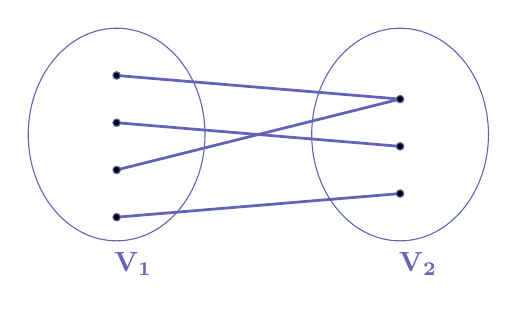
\begin{tikzpicture}[scale=0.3, hoccungpi]
			\draw [rotate around={90.:(5.,9.5)}] (5.,9.5) ellipse (4.5cm and 3.7416573867739413cm);
			\draw [rotate around={90.:(17.,9.5)}] (17.,9.5) ellipse (4.5cm and 3.7416573867739413cm);
			\draw [line width=1.pt] (5.,12.)-- (17.,11.);
			\draw [line width=1.pt] (5.,8.)-- (17.,11.);
			\draw [line width=1.pt] (5.,10.)-- (17.,9.);
			\draw [line width=1.pt] (5.,6.)-- (17.,7.);
			\draw (4.48,4.92) node[anchor=north west] {$\mathbf{V_1}$};
			\draw (16.54,4.94) node[anchor=north west] {$\mathbf{V_2}$};
			\begin{scriptsize}
				\draw [fill=black] (5.,12.) circle (4.5pt);
				\draw [fill=black] (5.,10.) circle (4.5pt);
				\draw [fill=black] (5.,8.) circle (4.5pt);
				\draw [fill=black] (5.,6.) circle (4.5pt);
				\draw [fill=black] (17.,11.) circle (4.5pt);
				\draw [fill=black] (17.,9.) circle (4.5pt);
				\draw [fill=black] (17.,7.) circle (4.5pt);
			\end{scriptsize}
		\end{tikzpicture}
		\caption{\small\textit{\color{hoccungpi} Hình $4.$ Minh họa đồ thị lưỡng phân.}}
		\vspace*{-10pt}
	\end{figure}
	Đồ thị lưỡng phân có những tính chất tương đối dễ thấy. Ví dụ, nếu tập đỉnh  $V$ được phân hoạch thành hai tập hợp $V_1, V_2$, thì $
	\sum\limits_{v \in V_1} \text{deg} (v) =  \sum\limits_{v \in V_2} \text{deg} (v) = |E|.$ Ngoài ra, số cạnh của đồ thị lưỡng phân $\pazocal{G}$ không vượt quá $|V_1| |V_2|$. Khi dấu bằng xảy ra, ta còn gọi đồ thị $\pazocal{G}$ là một đồ thị lưỡng phân đầy đủ và ký hiệu là $K_{a,b}$, với $a,b$ lần lượt là số phần tử của $V_1$, $V_2$.
	Tiếp theo, ta có một định lý để kiểm tra một đồ thị có là đồ thị lưỡng phân hay không. 
	\vskip 0.1cm
	\textbf{\color{hoccungpi}Định lý} $\pmb{3.1}$ (Dấu hiệu nhận biết)\textbf{\color{hoccungpi}.} 
		Cho  $\pazocal{G} = (V,E)$ là một đồ thị liên thông. Khi đó, các phát biểu sau là tương đương:
		\vskip 0.1cm
		$1.$ Đồ thị $\pazocal{G}$ lưỡng phân.
		\vskip 0.1cm
		$2.$ Các đỉnh của đồ thị $\pazocal{G}$ có thể tô bằng hai màu, sao cho hai đỉnh kề nhau không cùng màu.
		\vskip 0.1cm
		$3.$ Đồ thị $\pazocal{G}$ không chứa chu trình có số cạnh là lẻ.
		\vskip 0.1cm
	\textit{Chứng minh.} Ta dễ thấy rằng phát biểu $(1)$ tương đương với phát biểu $(2)$ vì $\pazocal{G}$ lưỡng phân tương đương với việc tập đỉnh của nó được phân hoạch thành hai tập $A,B$ mà mọi cạnh của $\pazocal{G}$ đều có một đầu mút thuộc $A$, một đầu thuộc $B$; và ta có thể tô các đỉnh thuộc $A$ bằng màu đen và các đỉnh thuộc $B$ màu trắng.
	\vskip 0.1cm
	Tiếp theo, ta chứng minh từ $(2)$ suy ra $(3)$. Nếu các đỉnh của $\pazocal{G}$ có thể được tô bằng hai màu sao cho hai đỉnh kề nhau bất kỳ khác màu mà có một chu trình lẻ cạnh thì dọc theo chu trình này, các đỉnh có màu đan xen nhau, vì thế đỉnh đầu và đỉnh cuối cùng màu, vô lý!
	\vskip 0.1cm
	Đảo lại, nếu $\pazocal{G}$ không chứa chu trình có số lẻ cạnh, ta có thể tô màu các đỉnh của nó như sau. Chọn một đỉnh gốc $u$ và tô đen, với mỗi đỉnh $v$, lấy tùy ý một đường đi từ $u$ đến $v$ (đường đi này luôn tồn tại vì $\pazocal{G}$ liên thông). Nếu đường đi này độ dài chẵn thì tô $v$ màu đen, nếu lẻ thì tô $v$ màu trắng. Cách tô này không phụ thuộc vào việc lựa chọn đường đi nào, vì mọi đường đi từ $u$ đến $v$ phải cùng tính chẵn lẻ, nếu không  bằng cách ghép một đường đi độ dài chẵn với một đường đi độ dài lẻ, ta thu được một chu trình độ dài lẻ. Hơn nữa, có thể thấy ngay cách tô này đảm bảo hai đỉnh kề nhau không cùng màu. 
	\vskip 0.1cm
	\textit{Lưu ý.} Giả thiết đồ thị $\pazocal{G}$ liên thông chỉ giúp ta dễ dàng hơn trong việc trình bày chứng minh trên. Kết quả của định lý trên vẫn đúng nếu ta bỏ đi giả thiết $\pazocal{G}$ liên thông. Tiếp theo, ta cùng xét một số ví dụ minh họa. 
	\vskip 0.1cm
	\textbf{\color{hoccungpi}Ví dụ} $\pmb{3.1}$ (Olympic Canada năm $2019$)\textbf{\color{hoccungpi}.} 
	Cho $n \geq 3$ điểm trên mặt phẳng sao cho không có ba điểm nào thẳng hàng. Hai người chơi một trò chơi như sau. Họ luân phiên chơi. Ở mỗi lượt chơi, người đến lượt chọn hai điểm chưa được nối và nối chúng lại với nhau. Người đầu tiên tạo ra một chu trình có số cạnh là lẻ thua cuộc. Tìm tất cả các giá trị của $n$ sao cho người chơi đầu tiên có chiến lược thắng cuộc.  
	\vskip 0.1cm
	\textbf{\color{hoccungpi}Nhận xét. } Mô hình đồ thị là rất rõ trong bài toán này. Do bài toán đề cập đến chu trình lẻ cạnh, nên ta nghĩ đến cấu trúc đồ thị lưỡng phân.  
	\vskip 0.1cm
	\textit{Lời giải.} Gọi hai người chơi là $A, B$ và giả sử $A$ là người chơi đầu tiên.
	\vskip 0.1cm
	Ở mọi thời điểm, khi người chơi vẫn có thể nối thêm một đường, thì đồ thị $\pazocal{G}$ vẫn chưa chứa chu trình lẻ cạnh. Do đó, nó vẫn là đồ thị lưỡng phân. Vì vậy, nếu người chơi $P$ thua, nghĩa là ở lượt chơi tiếp theo, với mọi cách nối hai điểm chưa được nối với nhau, anh ta đều tạo ra một đồ thị không còn là đồ thị lưỡng phân. Nói cách khác, đồ thị $\pazocal{G}$ ở thời điểm đó phải là đồ thị lưỡng phân đầy đủ $K_{a,b}$; với $a,b$ là các số nguyên không âm thỏa mãn $a+b =n$. Vì vậy, số cạnh của $\pazocal{G}$ khi đó là $ab$.
	\vskip 0.1cm
	Để $A$ giành chiến thắng, rõ ràng $ab$ phải là số lẻ. Nếu $n$ lẻ, thì chắc chắn một trong hai số $a,b$ chẵn. Suy ra $ab$ chẵn, và $A$ sẽ thua. 
	\vskip 0.1cm
	Nếu $n$ chẵn, chúng ta dự đoán trạng thái cuối cùng của đồ thị $\pazocal{G}$ sẽ là $K_{n/2,n/2}$ nếu cả $A$ và $B$ đều chơi một cách tối ưu. Vì vậy, nếu $n \equiv 0$ (mod $4$) thì $a=b = n/2$ đều chẵn và $A$ thua. Nếu $n \equiv 2$ (mod $4$) thì $a=b=n/2$ đều lẻ và $A$ thắng. Bây giờ, chúng ta sẽ chứng minh dự đoán trên.
	\vskip 0.1cm
	Chúng ta sẽ gọi một đồ thị lưỡng phân liên thông là {\it cân bằng} nếu các tập đỉnh đen và trắng  của nó (như trong Định lý $3.1$) của nó có lực lượng bằng nhau. (Điều kiện liên thông đảm bảo rằng cách tô màu là duy nhất, sai khác hoán vị các màu.) Tổng quát, một đồ thị hai phần được gọi là cân bằng nếu mỗi thành phần liên thông có nhiều hơn $1$ đỉnh của nó là cân bằng.
	\vskip 0.1cm
	Chiến lược chơi của người thắng cuộc là đảm bảo rằng sau mỗi lần anh ta chơi, đồ thị luôn là cân bằng và nói riêng số các đỉnh độc lập luôn là số chẵn.
	\vskip 0.1cm
	\textit{Trường hợp $1$: $n \equiv 2 \pmod 4$.} Người chơi $A$ có thể sử dụng chiến lược sau đây để đưa $\pazocal{G}$ về dạng $K_{n/2,n/2}$, và giành chiến thắng. Nhắc lại rằng, khi trò chơi chưa kết thúc, đồ thị là lưỡng phân. Hiển nhiên rằng ở nước đi đầu tiên $A$ sẽ nối $2$ đỉnh nào đó lại với nhau và do đó sau nước đi này thì đồ thị là cân bằng và số đỉnh cô lập là số chẵn. Ở mỗi lượt chơi sau đó của mình, tùy theo cách chơi của $B$ mà $A$ sẽ có cách chơi tương ứng:
	\vskip 0.1cm
	$\bullet$ Nếu $B$ nối một đỉnh cô lập với một đỉnh $S$ nào đó thuộc một thành phần liên thông không tầm thường (của đồ thị cân bằng đang có sau nước đi của $A$) thì $A$ sẽ nối một đỉnh cô lập khác với một đỉnh $T$ thuộc thành phần liên thông đó sao cho $S$ và $T$ có màu khác nhau.
	\vskip 0.1cm
	$\bullet$ Nếu $B$ nối $2$ đỉnh cô lập với nhau, hoặc nối $2$ đỉnh khác màu của một thành phần liên thông, hoặc nối $1$ đỉnh của một thành phần liên thông với $1$ đỉnh của một thành phần liên thông khác thì sau nước đi của $B$, đồ thị vẫn là cân bằng (và có số đỉnh cô lập là số chẵn). Khi này, $A$ chỉ cần nối $2$ đỉnh cô lập (nếu có) hoặc $2$ đỉnh không cô lập bất kỳ miễn là chúng không cùng màu.
	\vskip 0.1cm
	Ta dễ dàng kiểm tra được rằng cách chơi của $A$ đảm bảo rằng đồ thị luôn là cân bằng và đồ thị cuối cùng mà anh ta nhận được là $K_{n/2, n/2}$. 
	\vskip 0.1cm
	\textit{Trường hợp $2$: $n\equiv 0\pmod 4$.} Người chơi $B$ có thể sử dụng chiến lược giống hệt người chơi $A$ để đưa $\pazocal{G}$ về dạng  $K_{n/2,n/2}$, và giành chiến thắng.      
	\vskip 0.1cm
	Vậy người chơi $A$ có chiến lược  thắng khi và chỉ khi $n$ chia $4$ dư $2$.  
	\vskip 0.1cm
	\textbf{\color{hoccungpi}Ví dụ $\pmb{3.2}$} (Olympic Trung Quốc năm $2021$)\textbf{\color{hoccungpi}.}
	Một hội nghị có $n>3$ nhà khoa học, một số họ là bạn của nhau (quan hệ bạn bè là hai chiều và không có ai là bạn của chính bản thân mình). Người ta nhận thấy rằng, với mọi cách phân hoạch các nhà khoa học thành hai tập hợp khác rỗng, luôn tồn tại  hai người cùng thuộc một tập là bạn của nhau và hai người không cùng thuộc một tập là bạn của nhau.
	\vskip 0.1cm
	Trong ngày đầu tiên, mỗi nhà khoa học đưa ra một số nguyên không âm. Ở ngày thứ $k$, mỗi nhà khoa học thay đổi con số của mình bằng phần nguyên của trung bình cộng của các số của tất cả các bạn của mình trong ngày $k-1$. Chứng minh rằng, sau một số hữu hạn ngày, tất cả các nhà khoa học sẽ cùng đưa ra một con số.    
	\vskip 0.1cm
	\textit{Lời giải.}
	Chúng ta sẽ sử dụng mô hình đồ thị $\pazocal{G} = (V,E)$, trong đó mỗi nhà khoa học là một đỉnh và hai đỉnh nối với nhau nếu hai nhà khoa học này là bạn của nhau. Ta có $7$ nhận xét nhỏ như sau:
	\vskip 0.1cm
	$1.$ Đồ thị $\pazocal{G}$ liên thông. Thật vậy, giả sử $\pazocal{G}$ có ít nhất hai thành phần liên thông; gọi $S$ là một trong các thành phần liên thông. Xét phân hoạch $(V, V \setminus S)$: phân hoạch này không chứa hai người khác tập nhưng là bạn của nhau, mâu thuẫn.
	\vskip 0.1cm
	$2.$ Đồ thị $\pazocal{G}$ không là đồ thị lưỡng phân, vì nếu nó là đồ thị lưỡng phân thì ta phân hoạch tập đỉnh thành hai phía tương ứng. Khi đó, sẽ không tồn tại hai người là bạn của nhau cùng thuộc một tập. Điều này kéo theo đồ thị $\pazocal{G}$ phải chứa chu trình có số lẻ cạnh. Gọi một chu trình như vậy là $(P)$. 
	\vskip 0.1cm
	$3.$  Nhận xét trên kéo theo, giữa hai đỉnh bất kỳ $u,v$, tồn tại một đường đi từ $u$ đến $v$ có một số chẵn cạnh. Thật vậy, lấy một đỉnh $w$ thuộc chu trình $(P)$. Xét một đường đi có dạng $u-w-v$. Nếu đường đi này có một số chẵn cạnh thì ta có điều phải chứng minh; nếu nó có một số lẻ cạnh thì ta xét đường đi $u-w(P)w-v$, nghĩa là đường đi như trên, bổ sung thêm đường đi quanh $w$ bằng chu trình $(P)$: vì $(P)$ có một số lẻ cạnh nên nên đường đi này có một số chẵn cạnh. 
	\vskip 0.1cm
	$4.$ Xét dãy $(a_n)$, trong đó $a_n$ là số lớn nhất ở ngày thứ $n$. Dãy này  không tăng. Thật vậy, giả sử các nhà khoa học ở ngày thứ $n$ có số lớn nhất là $a_n$. Khi đó ở ngày $n+1$, mỗi nhà khoa học có số mới là trung bình cộng của các bạn của mình nên nó nhỏ hơn hoặc bằng $a_n$.
	\vskip 0.1cm
	$5.$  Mặt khác, dãy số nguyên $(a_n)$ bị chặn dưới bởi $0$, nên nó có giới hạn bằng $M$. Điều này có nghĩa là kể từ ngày thứ $N$ đủ lớn nào đó, ta luôn có $a_n = M$ với mọi $n \geq N$. 
	\vskip 0.1cm
	$6.$  \textit{Kể từ ngày thứ $N$, tất cả các nhà khoa học đều có số là $M$.} Để chỉ ra điều đó, ta sử dụng phương pháp phản chứng. Giả sử tồn tại nhà khoa học $v$ có số nhỏ hơn $M$ ở ngày thứ $k>N$, khi đó ở ngày thứ $k+1$, số của tất cả các bạn của $v$ sẽ nhỏ hơn $M$. Gọi khoảng cách giữa $2$ đỉnh (của một đồ thị liên thông) là số cạnh của đường đi ngắn nhất (sử dụng ít cạnh nhất) giữa chúng, ta sẽ có một dãy các sự kiện ở các ngày tiếp theo như sau:
	\vskip 0.1cm
	$\bullet$ Ở ngày $k+1$, tất cả các đỉnh có khoảng cách bằng $1$ đến $v$ đều có  số nhỏ hơn $M$.
	\vskip 0.1cm
	$\bullet$ Ở ngày $k+2$, tất cả các đỉnh có khoảng cách bằng $0,2$ đến $v$ đều có  số nhỏ hơn $M$.
	\vskip 0.1cm
	$\bullet$ Ở ngày $k+3$, tất cả các đỉnh có khoảng cách bằng $1,3$ đến $v$ đều có số nhỏ hơn $M$.
	\vskip 0.1cm
	\dots
	\vskip 0.1cm Ở ngày $k+2l$, tất cả các đỉnh có khoảng cách bằng $0,2,\dots,2l$ đến $v$ đều có số nhỏ hơn $M$.
	\vskip 0.1cm  
	$7.$ Tuy nhiên, vì giữa hai đỉnh $u,v$ bất kỳ đều tồn tại một đường đi có số chẵn cạnh, nên với $l$ đủ lớn, ở ngày $k+2l$, tất cả các nhà khoa học đều có số nhỏ hơn $M$, mâu thuẫn!!!  
	\vskip 0.1cm 
	Như vậy, ta có điều cần chứng minh.
	\vskip 0.1cm
	Trong các đồ thị lưỡng phân, có một loại đồ thị đặc biệt. Ỏ phần tiếp theo, ta sẽ cùng tìm hiểu loại đồ thị này. 
	\vskip 0.1cm
%	$\pmb{4.}$ \textbf{\color{hoccungpi}Đồ thị cây}
%	\vskip 0.1cm
%	Trong một số tình huống, ta có thể gặp những đồ thị mà số cạnh rất ít (còn gọi là đồ thị thưa). Khi đó, cấu trúc \textit{đồ thị cây} thường sẽ xuất hiện. Ta có định nghĩa về đồ thị cây như sau.
%	\vskip 0.1cm
%	\textbf{\color{hoccungpi}Định nghĩa} $\pmb{4.1}$ (Cây)\textbf{\color{hoccungpi}.}
%	Một đồ thị được gọi là một \textit{cây} nếu nó liên thông và không chứa một chu trình nào. 
%	\begin{figure}[H]
%		\vspace*{-5pt}
%		\centering
%		\captionsetup{labelformat= empty, justification=centering}
%		\definecolor{qqqqff}{rgb}{0.,0.,1.}
%		\begin{tikzpicture}[scale=0.4, hoccungpi]
%			\clip(3.52,0.5) rectangle (17.14,10.78);
%			\draw [line width=1.2pt] (9.,1.)-- (9.,4.);
%			\draw [line width=1.2pt] (9.,4.)-- (6.,7.);
%			\draw [line width=1.2pt] (6.,7.)-- (4.,10.);
%			\draw [line width=1.2pt] (6.,7.)-- (8.,10.);
%			\draw [line width=1.2pt] (9.,4.)-- (12.,10.);
%			\draw [line width=1.2pt] (9.,4.)-- (15.,7.);
%			\draw [line width=1.2pt] (15.,7.)-- (13.,10.);
%			\draw [line width=1.2pt] (15.,7.)-- (16.,10.);
%			\begin{scriptsize}
%				\draw [fill=qqqqff] (9.,1.) circle (5pt);
%				\draw [fill=qqqqff] (9.,4.) circle (5pt);
%				\draw [fill=qqqqff] (6.,7.) circle (5pt);
%				\draw [fill=qqqqff] (4.,10.) circle (5pt);
%				\draw [fill=qqqqff] (8.,10.) circle (5pt);
%				\draw [fill=qqqqff] (12.,10.) circle (5pt);
%				\draw [fill=qqqqff] (9.,4.) circle (5pt);
%				\draw [fill=qqqqff] (15.,7.) circle (5pt);
%				\draw [fill=qqqqff] (13.,10.) circle (5pt);
%				\draw [fill=qqqqff] (16.,10.) circle (5pt);
%			\end{scriptsize}
%		\end{tikzpicture}
%		\caption{\small\textit{\color{hoccungpi} Hình $5.$ Minh họa đồ thị cây.}}
%		\vspace*{-10pt}
%	\end{figure}
%	Lưu ý rằng, một đồ thị cây không chứa chu trình, do đó nó không thể chứa một chu trình lẻ cạnh, hay một đồ thị cây cũng đồng thời là một đồ thị lưỡng phân. Nếu đồ thị $\pazocal{G}$ gồm một số thành phần liên thông, mà mỗi thành phần liên thông là một cây, thì $\pazocal{G}$ còn được gọi là một \textit{rừng}. Ta có định lý sau:
%	\vskip 0.1cm 
%	\textbf{\color{hoccungpi}Định lý} $\pmb{4.1}$ (Các đặc trưng tương đương của cây)\textbf{\color{hoccungpi}.}
%	Cho  $\pazocal{G}$ là một đồ thị có $n$ đỉnh. Khi đó, các phát biểu sau là tương đương:
%	\vskip 0.1cm
%	$1.$ $\pazocal{G}$ là một cây;
%	\vskip 0.1cm
%	$2.$ $\pazocal{G}$ không có chu trình và có $n-1$ cạnh;
%	\vskip 0.1cm
%	$3.$ $\pazocal{G}$ liên thông và có $n-1$ cạnh;
%	\vskip 0.1cm
%	$4.$ $\pazocal{G}$ không có chu trình và nếu bổ sung vào một cạnh nối hai đỉnh không kề nhau thì xuất hiện một chu trình duy nhất;
%	\vskip 0.1cm
%	$5.$ $\pazocal{G}$ liên thông và nếu bỏ đi một cạnh bất kỳ thì $\pazocal{G}$ mất tính liên thông;
%	\vskip 0.1cm
%	$6.$ Mỗi cặp đỉnh trong $\pazocal{G}$ được nối với nhau bằng một đường đi duy nhất.
%	\vskip 0.1cm
%	Việc chứng minh định lý trên không khó. Bạn đọc quan tâm có thể tìm hiểu chi tiết chứng minh trong [$4$]. Để minh họa, chúng ta hãy cùng xét hai ví dụ sau.
%	\vskip 0.1cm
%	\textbf{\color{hoccungpi}Ví dụ} $\pmb{4.1}$ (Bài toán dự tuyển thi IMO  năm $2019$, Croatia đề xuất)\textbf{\color{hoccungpi}.}
%	Trong một mạng xã hội, có $2019$ người dùng, một số họ là bạn của nhau (quan hệ bạn bè là quan hệ $2$ chiều). Ban đầu, có $1010$ người mà mỗi người có đúng $1009$ bạn và có $1009$ người mà mỗi người có đúng $1010$ bạn. Tuy nhiên, quan hệ bạn bè trong mạng này không bền vững, những sự kiện tương tự như sự kiện sau có thể lần lượt xảy ra (mỗi thời điểm chỉ có đúng một sự kiện xảy ra):
%	\vskip 0.1cm
%	Ký hiệu $A,B,C$ là ba người dùng sao cho $A$ là bạn của cả $B$ và $C$, nhưng $B$ và $C$ không phải là bạn của nhau. Khi đó $B$ và $C$ sẽ trở thành bạn, đồng thời $A$ không còn là bạn của cả $B$ và $C$.
%	\vskip 0.1cm
%	Chứng minh rằng, với mọi cấu hình ban đầu, tồn tại một dãy các sự kiện như sự kiện trên mà sau đó, mỗi người dùng chỉ còn tối đa một người bạn.  
%	\vskip 0.1cm
%	\textbf{\color{hoccungpi}Nhận xét. } Bài toán trên rõ ràng có thể phát biểu lại bằng ngôn ngữ của lý thuyết đồ thị như sau. Cho một đồ thị $\pazocal{G}$ có $2019$ đỉnh. Trong đó, $1010$ đỉnh có bậc $1009$ và $1009$ đỉnh có bậc $1010$. Ở mỗi bước, ta có thể: \textit{``Chọn ra ba đỉnh $A,B,C$ mà $A$ nối với cả $B$ và $C$; còn $B,C$ không nối với nhau. Sau đó, xóa hai cạnh $AB,AC$ và thêm cạnh $BC$ vào đồ thị $\pazocal{G}$.''}
%	\vskip 0.1cm
%	Gọi mỗi thao tác trên là một thao tác \textit{đảo cạnh}. Ta cần chứng minh rằng, thông qua một dãy các thao tác đảo cạnh, ta có thể tạo ra một đồ thị mà mỗi đỉnh của đồ thị có bậc không vượt quá $1$. Không khó để nhận ra, đây chính là một đồ thị rừng. 
%	\vskip 0.1cm
%	\textit{Lời giải.}
%	Chú ý rằng một thao tác đảo cạnh bảo toàn tính chất: đồ thị $\pazocal{G}$ có ít nhất một đỉnh bậc lẻ và không phải là một đồ thị đầy đủ (tính chất này là hiển nhiên). Ta cũng chú ý rằng, đồ thị ban đầu là liên thông (chứng minh được dành cho bạn đọc như một bài tập). Bây giờ, ta mô tả một thuật toán gồm hai bước để chuyển đồ thị ban đầu về một đồ thị mà bậc của mỗi đỉnh không vượt quá $1$. 
%	\vskip 0.1cm
%	\textit{Bước $1$: Tồn tại một dãy các thao tác đảo cạnh để chuyển đồ thị ban đầu về một đồ thị dạng cây.}
%	\vskip 0.1cm
%	\textit{Chứng minh.} Vì số cạnh của đồ thị giảm đi $1$ sau mỗi thao tác đảo cạnh, ta chỉ cần chứng minh: chừng nào đồ thị $\pazocal{G}$ còn chứa một chu trình, thì tồn tại một thao tác đảo cạnh sao cho đồ thị mới được tạo ra vẫn liên thông. Ta đi chứng minh đồ thị chứa một chu trình $\pazocal{Z}$ và các đỉnh $A,B,C$ sao cho hai đỉnh $A$ và $B$ kề nhau trong chu trình $\pazocal{Z}$, đỉnh $C$ không nằm trong chu trình $\pazocal{Z}$ và kề với đỉnh $A$ nhưng không kề với đỉnh $B$. Bỏ hai cạnh $AB, AC$ và thêm cạnh $BC$ sẽ bảo toàn tính liên thông của đồ thị và khẳng định được chứng minh.  
%	\begin{figure}[H]
%		\vspace*{-5pt}
%		\centering
%		\captionsetup{labelformat= empty, justification=centering}
%		\definecolor{qqqqff}{rgb}{0.,0.,1.}
%		\begin{tikzpicture}[scale=0.25,hoccungpi]
%			\draw (18.,30.)-- (12.,24.);
%			\draw (12.,24.)-- (18.,18.);
%			\draw (18.,18.)-- (26.,18.);
%			\draw (26.,18.)-- (32.,24.);
%			\draw (32.,24.)-- (26.,30.);
%			\draw (26.,30.)-- (18.,30.);
%			\draw (32.,24.)-- (38.,30.);
%			\draw [dash pattern=on 2pt off 2pt] (26.,30.)-- (38.,30.);
%			\draw (32.1,24.2) node[anchor=north west] {$A$};
%			\draw (25.5,32) node[anchor=north west] {$B$};
%			\draw (37.6,32) node[anchor=north west] {$C$};
%			\begin{scriptsize}
%				\draw [fill=qqqqff] (18.,30.) circle (5pt);
%				\draw [fill=qqqqff] (12.,24.) circle (5pt);
%				\draw [fill=qqqqff] (18.,18.) circle (5pt);
%				\draw [fill=qqqqff] (26.,18.) circle (5pt);
%				\draw [fill=qqqqff] (32.,24.) circle (5pt);
%				\draw [fill=qqqqff] (26.,30.) circle (5pt);
%				\draw [fill=qqqqff] (38.,30.) circle (5pt);
%			\end{scriptsize}
%		\end{tikzpicture}
%		\caption{\small\textit{\color{hoccungpi}Hình $6.$ Nếu đồ thị $\pazocal{G}$ chứa chu trình $\pazocal{Z}$, thì ta vẫn có thể giảm số cạnh của nó.}}
%		\vspace*{-10pt}
%	\end{figure}
%	Để tìm chu trình $\pazocal{Z}$ và các đỉnh $A,B,C$; ta sử dụng hai chiến lược sau. Nếu đồ thị $\pazocal{G}$ chứa một tam giác, ta xét một đồ thị con đầy đủ lớn nhất $K$. Rõ ràng $K$ chứa ít nhất ba đỉnh. Vì đồ thị $\pazocal{G}$ không là đồ thị đầy đủ, tồn tại một đỉnh $C$ không thuộc $K$ và kề với một đỉnh $A$ thuộc $K$. Do tính lớn nhất của $K$, có một đỉnh $B$ thuộc $K$ không kề với đỉnh $C$, và do đó ta có thể chọn chu trình $\pazocal{Z}$ trong $K$ và đi qua cạnh $AB$. 
%	\vskip 0.1cm
%	Nếu đồ thị $\pazocal{G}$ không chứa tam giác, ta xét một chu trình ngắn nhất $\pazocal{Z}$ trong đồ thị $\pazocal{G}$. Chu trình này không thể là một chu trình Hamilton (tức là chu trình đi qua tất cả các đỉnh của đồ thị, mỗi đỉnh đúng một lần). Thật vậy, nếu không, do tính nhỏ nhất của $\pazocal{Z}$, đồ thị $\pazocal{G}$ sẽ không chứa thêm một cạnh nào nữa, dẫn đến mỗi đỉnh của đồ thị $\pazocal{G}$ đều có bậc bằng $2$, mâu thuẫn với việc đồ thị luôn có đỉnh bậc lẻ. Như vậy, $\pazocal{Z}$ không là một chu trình Hamilton và vì thế có thể tìm được một đỉnh $C$ không thuộc $\pazocal{Z}$ và kề với một đỉnh $A$ thuộc $\pazocal{Z}$. Do đồ thị $\pazocal{G}$ không chứa tam giác, đỉnh $C$ sẽ không kề với bất kỳ đỉnh $B$ nào kề với $A$ trong $\pazocal{Z}$ và ta chọn được chu trình $\pazocal{Z}$ và ba đỉnh $A,B,C$.    
%	\begin{figure}[H]
%		\vspace*{-5pt}
%		\centering
%		\captionsetup{labelformat= empty, justification=centering}
%		\definecolor{qqqqff}{rgb}{0.,0.,1.}
%		\definecolor{cqcqcq}{rgb}{0.7529411764705882,0.7529411764705882,0.7529411764705882}
%		\begin{tikzpicture}[scale=0.25, hoccungpi]
%			\draw (18.,30.)-- (12.,24.);
%			\draw (12.,24.)-- (18.,18.);
%			\draw (18.,18.)-- (26.,18.);
%			\draw (26.,18.)-- (32.,24.);
%			\draw (32.,24.)-- (26.,30.);
%			\draw (26.,30.)-- (18.,30.);
%			\draw (32.,24.)-- (38.,30.);
%			\draw [dash pattern=on 2pt off 2pt] (26.,30.)-- (38.,30.);
%			\draw (32.1,24.2) node[anchor=north west] {$A$};
%			\draw (25.5,32) node[anchor=north west] {$B$};
%			\draw (37.6,32) node[anchor=north west] {$C$};
%			\draw (18.,30.)-- (26.,18.);
%			\draw (26.,30.)-- (18.,18.);
%			\draw (12.,24.)-- (32.,24.);
%			\draw (18.,30.)-- (18.,18.);
%			\draw (26.,30.)-- (26.,18.);
%			\draw (12.,24.)-- (26.,30.);
%			\draw (26.,18.)-- (12.,24.);
%			\draw (18.,30.)-- (32.,24.);
%			\draw (32.,24.)-- (18.,18.);
%			\begin{scriptsize}
%				\draw [fill=qqqqff] (18.,30.) circle (5pt);
%				\draw [fill=qqqqff] (12.,24.) circle (5pt);
%				\draw [fill=qqqqff] (18.,18.) circle (5pt);
%				\draw [fill=qqqqff] (26.,18.) circle (5pt);
%				\draw [fill=qqqqff] (32.,24.) circle (5pt);
%				\draw [fill=qqqqff] (26.,30.) circle (5pt);
%				\draw [fill=qqqqff] (38.,30.) circle (5pt);
%			\end{scriptsize}
%		\end{tikzpicture}
%		\caption{\small\textit{\color{hoccungpi} Hình $7.$ Minh họa cách tìm chu trình $\pazocal{Z}$ và ba điểm $A,B,C$.}}
%		\vspace*{-10pt}
%	\end{figure} 
%	\textit{Bước $2$: Mọi đồ thị dạng cây đều có thể chuyển về một đồ thị có bậc mỗi đỉnh không vượt quá $1$ thông qua một dãy các thao tác đảo cạnh.}
%	\vskip 0.1cm
%	\textit{Chứng minh.} Để ý rằng thao tác đảo cạnh  bảo toàn tính chất không chứa chu trình. Do đó, kể từ một cây, sau các thao tác đảo cạnh, ta luôn có một đồ thị không chứa chu trình. Ngoài ra, mỗi thao tác đảo cạnh sẽ giảm số cạnh của đồ thị đi $1$ nên  đến một lúc nào đó ta không thể thực hiện thêm một thao tác đảo cạnh nào nữa. Khi này bậc của mỗi đỉnh của đồ thị này không vượt quá $1$. Thật vậy, nếu có một đỉnh $A$ với  kề với hai đỉnh $B,C$ nào đó (khi đó $B,C$ không kề nhau vì đồ thị đang xét không chứa chu trình) thì ta có thể thực hiện thêm một thao tác đảo cạnh.
%	\vskip 0.1cm
%	\textbf{\color{hoccungpi}Ví dụ} $\pmb{4.2}$ (Kỳ thi chọn đội tuyển Mỹ tham dự Egmo $2020$)\textbf{\color{hoccungpi}.} Cho $\pazocal{G}=(V,E)$ là một  đồ thị đơn có $n$ đỉnh. Một cạnh $e$ của của nó được gọi là một \textit{cạnh cổ chai} nếu có thể phân hoạch $V$ thành hai  tập $A,B$ thỏa mãn:
%	\vskip 0.1cm
%	$1.$ Có tối đa $100$ cạnh của $\pazocal{G}$ có một đầu mút thuộc $A$ và đầu mút còn lại thuộc $B$;
%	\vskip 0.1cm
%	$2.$ Cạnh $e$ là một trong số các cạnh như vậy.
%	\vskip 0.1cm 
%	Chứng minh rằng đồ thị $\pazocal{G}$ có tối đa $100(n-1)$ cạnh cổ chai.
%	\vskip 0.1cm
%	\textbf{\color{hoccungpi}Nhận xét. } Con số $100(n-1)$ ít nhiều gợi ý cho ta $100$ cấu trúc cây trong đồ thị $\pazocal{G}$. 
%	\vskip 0.1cm
%	\textit{Lời giải.} Gọi $F_1$ là một rừng lớn nhất trong $\pazocal{G}$ (nếu $\pazocal{G}$ liên thông thì $F_1$ chính là một cây). Xóa đi các cạnh của $F_1$ và gọi $F_2$ là rừng lớn nhất trong đồ thị mới nhận được (vẫn có $n$ đỉnh). Cứ tiếp tục như vậy, cho đến $F_{100}$ là rừng lớn nhất trong đồ thị nhận được khi xóa đi các cạnh của  $F_1\cup F_2\cup \cdots \cup F_{99}$. Giả sử ngược lại, $\pazocal{G}$ có nhiều hơn $100(n-1)$ cạnh cổ chai. Mỗi rừng $F_i$ (với $i=1,\dots,100$) (có $n$ đỉnh) có tối đa $n-1$ cạnh. Do vậy, tổng số các cạnh trong $F_1\cup F_2\cup \cdots \cup F_{100}$ không vượt quá $100(n-1)$. Vì vậy, vẫn tồn tại một cạnh cổ chai không nằm trong bất kỳ $F_{i}, i=1, 2, \ldots, 100$ nào.
%	Gọi $x-y$ là một cạnh như vậy ($x,y$ là hai đỉnh của đồ thị). Rõ ràng, trong mỗi $F_i$, có một đường đi từ $x$ đến $y$ vì nếu không, thêm cạnh $x-y$ vào $F_i$ ta vẫn có một rừng (mâu thuẫn với cách chọn $F_i$ lớn nhất). Vì vậy, trong $\pazocal{G}$ có ít nhất $101$ đường đi từ $x$ đến $y$, hơn nữa hai đường đi bất kỳ đều không có cạnh chung. Tuy nhiên, khi đó cạnh $x-y$ không thể là cạnh cổ chai. Thật vậy, gọi $A,B$ là phân hoạch của $V$ tương ứng với cạnh cổ chai $x-y$. Với mỗi $i$, đường đi  trong $F_i$ từ $x$ đến $y$ phải chứa một cạnh nối một đỉnh thuộc $A$ và một đỉnh thuộc $B$. Tóm tại, ta tìm được $101$ cạnh của $G$ mà một đầu mút thuộc $A$ và  đầu mút còn lại thuộc $B$ (mâu thuẫn với điều kiện $(1)$). 
%	\vskip 0.1cm
%	Hy vọng rằng qua một số lý thuyết và bài tập minh họa, bạn đọc đã ít nhiều thấy được tiềm năng, sự phong phú và mối liên hệ của lý thuyết đồ thị với nhiều mảng kiến thức khác. Rõ ràng, khi mô hình hóa được một bài toán dưới dạng ngôn ngữ đồ thị, ta có thể tìm ra định hướng tốt trong việc tìm kiếm lời giải. Cụ thể hơn, khi gặp một mô hình đồ thị có nhiều cạnh, ta có thể liên tưởng đến cấu trúc đồ thị lưỡng phân; ngược lại, một mô hình đồ thị ít cạnh làm chúng ta liên tưởng đến đồ thị dạng cây, rừng.  
%	Phần cuối của bài viết này là một số bài tập giúp rèn luyện thêm kỹ năng phát hiện và sử dụng các cấu trúc đồ thị lưỡng phân và cây.   
%	\vskip 0.1cm
%	$\pmb{5.}$ \textbf{\color{hoccungpi}Một số bài toán tự rèn luyện}
%	\vskip 0.1cm
%	\textbf{\color{hoccungpi}Bài $\pmb{1.}$} \textit{(Olympic Canada năm $2020$)} Cho đồ thị $\pazocal{G}$ có $19998$ đỉnh. Mỗi đồ thị con gồm $9999$ đỉnh của $\pazocal{G}$ đều chứa ít nhất $9999$ cạnh. Hỏi $\pazocal{G}$ có ít nhất bao nhiêu cạnh?
%	\vskip 0.1cm
%	\textbf{\color{hoccungpi}Bài $\pmb{2.}$}\textit{(Mở rộng Bài $2$)}  Cho đồ thị $\pazocal{G}$ có $2n$ đỉnh. Mỗi đồ thị con $n$ đỉnh của  $\pazocal{G}$ đều có ít nhất $n$ cạnh. Chứng minh rằng $\pazocal{G}$ có ít nhất $5n$ cạnh.
%	\vskip 0.1cm
%	\textbf{\color{hoccungpi}Bài $\pmb{3.}$} \textit{(Olympic Liên bang Nga năm $2004$)} Một quốc gia có $1001$ thành phố.  Hai thành phố bất kỳ được nối với nhau bằng một con đường một chiều. Mỗi thành phố có $500$ con đường đi ra và $500$ con đường đi vào. Có một tổ chức ly khai xuất hiện và chiếm đóng $668$ thành phố. Chứng minh rằng, trong khu vực ly khai này, từ mỗi thành phố đều có có thể đi đến một thành phố khác.
%	\vskip 0.1cm
%	\textbf{\color{hoccungpi}Bài $\pmb{4.}$}  Cho đồ thị $\pazocal{G} = (V,E)$ thỏa mãn $|E| = |V| +4$. Chứng minh rằng, trong $\pazocal{G}$ có
%	hai chu trình không có cạnh chung. 
	\vskip 0.1cm
	\textbf{\color{hoccungpi}Tài liệu}
	\vskip 0.1cm
	[$1$] Đỗ Đức Thái, \textit{Chuyên đề học tập toán $11$}. NXB Đại học Sư phạm Hà Nội. 
	\vskip 0.1cm
	[$2$] Hà Huy Khoái, \textit{Chuyên đề học tập toán $11$}. NXB Giáo dục Việt Nam. 
	\vskip 0.1cm
	[$3$] Asratian, Armen S.; Denley, Tristan M. J.; Häggkvist, Roland, \textit{Bipartite Graphs and their Applications}. Cambridge University Press, $1998$.
	\vskip 0.1cm
	[$4$] Bender, Edward A.; Williamson, S. Gill , \textit{Lists, Decisions and Graphs  With an Introduction to Probability}, $2010$.
	\vskip 0.1cm
	[$5$] Titu Andreescu, Bogdan Enescu, \textit{Mathematical Olympiad Treasures}. Springer, $2011$.
	\vskip 0.1cm                 
	[$6$] Website \url{https://artofproblemsolving.com}. 
\end{multicols}
%	\newpage
%
%	\thispagestyle{empty}
%	\begingroup 
%	\AddToShipoutPicture*{\put(0,0){\includegraphics[width=19.5cm]{MV.pdf}}}
%	\centering
%	\vspace*{0cm}
%	\endgroup
%	\newpage	
%	\pagestyle{empty}

	\setcounter{figure}{0}
	\thispagestyle{cackithitoannone}
\pagestyle{cackithitoan}
\everymath{\color{cackithi}}
\graphicspath{{../cackithi/pic/}}
\blfootnote{\color{cackithi}$^1$Khoa Toán Đại học Osnabrueck, CHLB Đức.}
\begingroup
\AddToShipoutPicture*{\put(0,616){\includegraphics[width=19.3cm]{../bannercackithi}}}
\AddToShipoutPicture*{\put(82,527){\includegraphics[scale=1]{../tieude2.pdf}}}
\centering
\endgroup
\vspace*{182pt}

%\begin{multicols}{2}
%	Trong chuyên mục này, chúng tôi sẽ trình bày Lời giải của các bài toán trong vòng hai kỳ thi toán học liên bang Đức năm $2023$, đăng trong số báo $9/2023$. 
%	\vskip 0.1cm
%	\textbf{\color{cackithi}Câu $\pmb{1}$:} Tìm ước chung lớn nhất của tất cả các số có dạng $p^6 - 7p^2 +6$ với $p$ chạy trên tập tất cả các số nguyên tố và $p \ge 11$.
%	\vskip 0.1cm
%	\textit{Lời giải.}
%	Đặt $f(p) \colon =p^6 - 7p^2 +6$. Gọi $a$ là ước chung lớn nhất (ƯCLN) của tất cả các $f(p)$ với $p$ nguyên tố và $p \ge 11$. Ta sẽ chứng minh rằng $a = 2^5\times 3 \times 7$.
%	\vskip 0.1cm	
%	Thật vậy, theo định lý Fermat nhỏ thì $7|p^6 - 1$ với mọi số nguyên $7 \not | p$. Do đó, $7 |p^6 - 1  - 7p^2 + 7 = f(p)$ với mọi $p$ như trên và ta có $7 | a$.
%	\vskip 0.1cm	
%	Mặt khác, 
%	$f(p) = (p^2-1)(p^2-2)(p^2+3) \equiv (p^2-1)(p^2-2)p^2 \mod 3 \equiv 0 \mod 3$ do $p^2, p^2-1, p^2-2$ là ba số nguyên liên tiếp. Như vậy, $3 | f(p)$ với mọi $p$ và ta thu được $3|a$.
%	\vskip 0.1cm	
%	Hơn nữa, do $p$ nguyên tố và $p \ge 11$ nên $p$ là số lẻ. Đặt $p= 2k+1$, ta có
%	\begin{align*}
%			f(p) = & (p^2-1)(p^2-2)(p^2+3) \\
%			= & (4k^2 \!+\! 4k) \!(4k^2 \!+\! 4k\!-\!1)(4k^2\!+\!4k\!+\!4) \\
%			= & 16k(k\!+\!1)(4k^2 \!+\! 4k\!-\!1)(k^2 \!+\! k \!+\! 1).
%	\end{align*}
%	Vì $2 |k(k+1)$ với mọi $k \in \mathbb{Z}$ nên $2\times 16 = 32 = 2^5 |f(p)$. Bởi vậy $2^5 |a$.
%	\vskip 0.1cm
%	Do $2^5, 3$ và $7$ đôi một nguyên tố cùng nhau nên
%	\begin{align*}
%		2^5 \times 3 \times 7 |a. \tag{$1$}
%	\end{align*}
%		Mặt khác, vì
%		$
%		f(11) = 1770720 = 2^5 \times 3 \times 5 \times 7 \times 17 \times 31
%		$
%		và
%		$
%		f(13) = 4825632 = 2^5 \times 3 \times 7 \times 43 \times 167
%		$
%		nên 
%		\begin{align*}
%			a |\text{ƯCLN}(f(11), f(13)) \!=\! 2^5\!\times\! 3 \!\times\! 7. \tag{$2$}
%		\end{align*}
%		Từ ($1$) và ($2$) ta thu được $a = 2^5\times 3 \times 7$.
%	\vskip 0.1cm
%	\textbf{\color{cackithi}Câu $\pmb{2}$:} Trên một hòn đảo địa hình đồi núi có $2023$ điểm quan sát. Từ mỗi điểm quan sát có thể nhìn thấy ít nhất $42$ điểm quan sát khác. Với hai điểm quan sát bất kỳ $X$ và $Y$, luôn tồn tại một số nguyên dương $n$ và các điểm quan sát $A_1,  A_2, \ldots, A_{n+1}$ sao cho $A_1 = X$, $A_{n+1} = Y$ và mỗi cặp điểm liền kề $A_i$ với $A_{i+1}$ có thể quan sát được lẫn nhau với $i = 1, 2, \ldots, n$. Số $n$ nhỏ nhất như vậy được gọi là khoảng cách quan sát (Sichtabstand). 
%	\vskip 0.1cm
%	Xác định khoảng cách quan sát lớn nhất có thể có giữa hai cặp điểm quan sát thỏa mãn những điều kiện ở trên.
%	\vskip 0.1cm
%	\textit{Lời giải.}
%	Ta sẽ chứng minh rằng khoảng cách quan sát lớn nhất có thể là $140$.
%	\vskip 0.1cm	
%	Với hai điểm quan sát $X,Y$ trong bài, ta nói $A_1, \ldots, A_{n+1}$ là các điểm thuộc \textit{chuỗi quan sát} độ dài $n$ nối $X$ và $Y$. Để tìm một chuỗi quan sát có độ dài nhỏ nhất, ta chỉ cần xét trường hợp mỗi điểm quan sát trong chuỗi xuất hiện đúng một lần. Vì chỉ có hữu hạn điểm quan sát nên độ dài các chuỗi quan sát là hữu hạn (bị chặn trên bởi $2022$). Như vậy giữa tất cả các chuỗi quan sát nối $X$ và $Y$ luôn tồn tại chuỗi quan sát có độ dài ngắn nhất, và độ dài này chính là khoảng cách quan sát được định nghĩa ở trên. Do chỉ có hữu hạn các cặp điểm quan sát, tồn tại một cặp điểm có khoảng cách quan sát lớn nhất.
%	\vskip 0.1cm	
%	Cho trước một hệ thống tùy ý $M$ gồm $2023$ điểm quan sát thỏa mãn yêu cầu của bài toán. Chọn $X \in M$ bất kỳ và gọi $M_i$ tập các điểm quan sát có khoảng cách quan sát $i$ tới $X$. Ta cũng sẽ đặt $M_0 = \{X\}$. Do với bất kỳ $Y \in M$ luôn tồn tại một chuỗi quan sát nối $X$ và $Y$ nên các tập $M_i$ lập nên một phân hoạch của $M$. Nói cách khác, $M = \cup_{i}M_i$ và $M_i \cap M_j = \emptyset$ nếu $i\neq j$.
%	\vskip 0.1cm
%	Gọi $n(X)$ là chỉ số sao cho $M_{n(X)} \neq \emptyset$ và $M_i = \emptyset$ với mọi $i \ge n(X)$. Bằng định nghĩa, với mỗi $Y \in M_{n(X)}$ luôn tồn tại chuỗi quan sát ngắn nhất $A_1, \ldots A_{n(X) + 1}$ với $A_1 = X$ và $A_{n(X)+1} = Y$. Rõ ràng $A_i, A_{i+1}, \ldots, A_{j}$ cũng là chuỗi quan sát ngắn nhất giữa $A_i$ và $A_j$ với mọi $1 \le i <j \le n(X) + 1$. Nói riêng, $A_i \in M_{i-1}$ và ta có $M_i \neq \emptyset$ với mọi $i \le n(X)$.
%	\vskip 0.1cm	
%	Hơn nữa, từ mỗi điểm trong $M_i$ chỉ có thể quan sát được các điểm trong $M_{i-1}, M_i$ và $M_{i+1}$. Thật vậy, nếu từ $V \in M_i$ quan sát được $W \in M_j$ với $j \le i-2$ thì $V \in M_{j+1}$. Do đó, $V \in M_i \cap M_{j+1}$. Điều này vô lý vì $M_i \cap M_{j+1} = \emptyset$ do $j+1 \neq i$. Tương tự, từ $V \in M_i$ quan sát được $W \in M_j$ với $j \ge i+2$ cũng dẫn đến mâu thuẫn. Vì từ mỗi $V \in M_i$ có thể quan sát được ít nhất $42$ điểm khác và các điểm này nằm trong $M_{i-1}, M_i, M_{i+1}$ nên
%	\begin{align*}
%		|M_{i-1} \cup M_i \cup M_{i+1}| \ge 43.
%	\end{align*}
%	Từ $X \in M_0$ chỉ quan sát được các điểm trong $M_1$ và từ $Y \in M_{n(X)}$ chỉ quan sát được các điểm từ $M_{n(X)}$ và $M_{n(X)-1}$ nên
%	\begin{align*}
%		|M_0 \cup M_1| \ge 43 \text{ và } |M_{n(X)-1} \cup M_{n(X)}| \ge 43.
%	\end{align*}
%	\textbf{\color{cackithi}Khẳng định $\pmb{1}$:} \textit{Khoảng cách quan sát lớn nhất không thể lớn hơn $140$.} 
%	\vskip 0.1cm
%	Thật vậy, nếu $M_{141} \neq \emptyset$ thì 
%	\begin{align*}
%		& |M_0 \cup M_1| + |M_2 \cup M_3 \cup M_4| \\
%		&+ |M_5 \cup M_6 \cup M7| + \ldots \\
%		&+ |M_{137} \cup M_{138} \cup M_{139}| + |M_{140} \cup M_{141}| \\
%		\ge \,&43 + 46.43 + 43 = 2064 > 2023
%	\end{align*}
%	dẫn đến mâu thuẫn.
%	\vskip 0.1cm
%		\textbf{\color{cackithi}Khẳng định $\pmb{2}$:} \textit{Tồn tại một hệ thống điểm quan sát sao cho khoảng cách quan sát lớn nhất là $140$.} 
%		\vskip 0.1cm
%		Thật vậy, xây dựng $141$ tập không rỗng $M_i$ với $i = 0, \ldots, 140$ như trong Hình $1$, trong đó:
%		\vskip 0.1cm
%		\begin{figure}[H]
%				\vspace*{-5pt}
%				\centering
%				\captionsetup{labelformat= empty, justification=centering}
%			\resizebox{\columnwidth}{!}{\begin{tikzpicture}[node distance={15mm}, thick, main/.style = {draw, circle}, cackithi] 
%				\node[main, fill={rgb:orange,1;yellow,2;pink,5}] (1) {$A_0$}; 
%				\node[main, fill= teal!50] (2) [above right of=1] {$A_1^1$}; 
%				\node (3) [right = 5mm of 1] {$\vdots$};
%				
%				\node[main, fill= teal!50] (4) [below right of=1] {$A_1^{42}$}; 
%				\node[main, fill={rgb:orange,1;yellow,2;pink,5}] (5) [below right of=2] {$A_2$}; 
%				\node[main,fill=gray!50] (6) [above right of=5] {$A_3^1$}; 
%				\node (7) [right = 5mm of 5] {$\vdots$};
%				\node[main, fill=gray!50] (8) [below right of=5] {$A_3^{41}$}; 
%				\draw (1) -- (2); 
%				\draw (1) -- (3); 
%				\draw (1) -- (4); 
%				\draw (2) -- (3);
%				\draw (3) -- (4);
%				\draw (2) -- (5); 
%				\draw (3) -- (5); 
%				\draw (4) -- (5); 
%				\draw (5) -- (6);
%				\draw (5) -- (7);
%				\draw (5) -- (8);   
%				\draw (6) -- (7);
%				\draw (7) -- (8);
%				\node[main, fill={rgb:orange,1;yellow,2;pink,5}] (9) [below right of=6] {$A_4$};
%				\draw (6) -- (9);
%				\draw (7) -- (9); 
%				\draw (8) -- (9);  
%				\node[main, fill={rgb:orange,1;yellow,2;pink,5}] (10) [right = 5mm of 9] {$A_{138}$};
%				\draw[dashed] (9) -- (10);  
%				\node[main, fill= teal!50] (11) [above right of=10] {$A_{139}^1$}; 
%				\node (12) [right = 4mm of 10] {$\vdots$}; 
%				\node[main, fill= teal!50] (13) [below right of=10] {$A_{139}^{42}$}; 
%				\draw (10) -- (11);
%				\draw (10) -- (12);
%				\draw (10) -- (13);
%				\draw (11) -- (12);
%				\draw (12) -- (13);
%				\node[main, fill={rgb:orange,1;yellow,2;pink,5}] (14) [below right of=11] {$A_{140}$};
%				\draw (11) -- (14);
%				\draw (12) -- (14);
%				\draw (13) -- (14);
%			\end{tikzpicture}}
%			\caption{\small\textit{\color{cackithi}Hình $1$. Hệ thống điểm quan sát với khoảng cách quan sát lớn nhất $140$. Mỗi điểm $A_i^{\bullet}$ thuộc tập $M_i$ có thể quan sát được tất cả điểm trong $M_{i-1}, M_{i+1}$ cũng như các điểm còn lại trong $M_i$.}}
%			\vspace*{-10pt}
%		\end{figure}
%		\vskip 0.1cm		
%		$\bullet$ Mỗi tập $M_{3k}$ và $M_{3k+2}$ với $k = 0, \ldots, 46$ chỉ chứa một điểm quan sát.
%		\vskip 0.1cm
%		$\bullet$ Mỗi tập $M_{1}$ và $M_{139}$ có $42$ điểm quan sát.
%		\vskip 0.1cm
%		$\bullet$ Mỗi tập $M_{3k+1}$ với $k = 1, \ldots, 45$ có $41$ điểm quan sát.
%		\vskip 0.1cm
%		Độc giả có thể kiểm tra rằng hệ thống này có $2023$ điểm quan sát và thỏa mãn điều kiện của bài toán. Ở đó, điểm quan sát duy nhất trong $M_{140}$ có khoảng cách quan sát $140$ tới điểm quan sát duy nhất trong $M_0$.
%		\vskip 0.1cm
%	\textbf{\color{cackithi}Câu $\pmb{3}$:} Cho tam giác $AB$C với tâm đường tròn nội tiếp $I$. Gọi trung điểm của các cạnh $AC$ và $BC$ lần lượt là $M_b$ và $M_a$. Gọi giao điểm của đường thẳng $M_bI$ với đường thẳng $BC$ là $B'$ và giao điểm của đường thẳng $M_aI$ với đường thẳng $AC$ là $A'$. Biết rằng hai tam giác $ABC$ và $A'B'C$ có cùng diện tích. 
%	\vskip 0.1cm
%	Tìm giá trị có thể của góc $ACB$.\footnote{\color{cackithi}Trong số $09/2023$ chúng tôi đã sai sót khi yêu cầu tìm giá trị \textbf{\color{cackithi}lớn nhất} có thể của góc $ACB$. Thành thật xin lỗi các độc giả của Pi.}	
%		\begin{figure}[H]
%			\vspace*{-10pt}
%			\centering
%			\captionsetup{labelformat= empty, justification=centering}
%			\resizebox{\columnwidth}{!}{\begin{tikzpicture}
%				\tkzSetUpPoint[size=4,circle, fill= teal!50]
%				\tkzDefPoints{0/0/A,6/0/B,0.8/4/C}
%				
%				\tkzDefTriangleCenter[centroid](A,B,C)
%				\tkzGetPoint{G}
%				\tkzDefSpcTriangle[medial](A,B,C){Ma,Mb,Mc}
%				%\tkzLabelPoints(A,B,C)
%				\tkzDefTriangleCenter[in](A,B,C)
%				\tkzGetPoint{I}
%				
%				\tkzDefCircle[in](A,B,C) 
%				\tkzGetPoints{I}{i}
%				
%				\tkzInterLL(Mb,I)(B,C)
%				\tkzGetPoint{B1}
%				\tkzInterLL(Ma,I)(A,C)
%				\tkzGetPoint{A1}
%				\tkzDrawSegments(A,B B,C C,A)
%				\tkzDrawPoints(A1,B1)
%				\tkzLabelPoint[above left](A1){$A'$}
%				\tkzLabelPoint(B1){$B'$}
%				\tkzDrawLines[dashed](B1,Mb A1,Ma)
%				\tkzDrawSegments(B1,B A1,B1)
%				\tkzDrawCircle(I,i)
%				\tkzDrawPoints(I, Mb, Ma)
%				
%				\tkzDrawPoints(A,B,C)
%				
%				\tkzLabelPoint(I){$I$}
%				
%				\tkzLabelPoints[below left](A,Mb)
%				\tkzLabelPoints[above right](B,Ma)
%				\tkzLabelPoint[above](C){$C$}
%			\end{tikzpicture}}
%		\vspace*{-10pt}
%		\end{figure}
%		\textit{Lời giải.} Gọi độ dài các cạnh $AB$, $BC$ và $CA$ lần lượt là $c$, $a$, $b$. Đặt $\gamma \colon = \angle ACB$. Ta sẽ chứng minh rằng $\gamma = 60^{\circ}$.
%		\vskip 0.1cm
%		Thật vậy, từ $M_a$ vẽ đường thẳng song song với $AC$ và cắt $CI$ tại $P$. Vì $\angle CPM_a = \angle A'CI = \gamma/2$ nên tam giác $CM_aP$ cân tại $M_a$ và ta có $M_aP = M_aC = a/2 = M_aB$. Như vậy $P$ nằm trên đường tròn tâm $M_a$ bán kính $a/2$. Từ đó suy ra tam giác $BPC$ vuông tại $P$ và ta thu được 
%		\begin{align*}
%			CP = CB \cos (\gamma /2) = a \cos(\gamma/2).
%		\end{align*}
%		\begin{figure}[H]
%			\vspace*{-5pt}
%			\centering
%			\resizebox{\columnwidth}{!}{\begin{tikzpicture}[color= cackithi]
%				\tkzSetUpPoint[size=4, fill= teal!50]
%				
%				\tkzDefPoints{0/0/A,6/0/B,0.8/4/C}
%				
%				\tkzDefTriangleCenter[centroid](A,B,C)
%				\tkzGetPoint{G}
%				\tkzDefSpcTriangle[medial](A,B,C){Ma,Mb,Mc}
%				%\tkzLabelPoints(A,B,C)
%				\tkzDefTriangleCenter[in](A,B,C)
%				\tkzGetPoint{I}
%				
%				\tkzDefCircle[in](A,B,C) 
%				\tkzGetPoints{I}{i}
%				
%				\tkzInterLL(Mb,I)(B,C)
%				\tkzGetPoint{B1}
%				\tkzInterLL(Ma,I)(A,C)
%				\tkzGetPoint{A1}
%				\tkzDrawSegments(A,B B,C C,A)
%				\tkzDrawPoint(A1)
%				\tkzLabelPoint[above left](A1){$A'$}
%				\tkzDrawLine[dashed](A1,Ma)
%				\tkzDrawCircle(I,i)
%				\tkzDrawPoints(I, Mb, Ma)
%				
%				\tkzDrawPoints(A,B,C)
%				
%				\tkzLabelPoint(I){$I$}
%				
%				\tkzAutoLabelPoints[center = G](A,B,C)
%				\tkzLabelPoint[below left](Mb){$M_b$}
%				\tkzLabelPoint[above right](Ma){$M_a$}
%				\tkzLabelPoint[below right](Mc){$M_c$}
%				\tkzInterLL(C,I)(Ma,Mc)
%				\tkzGetPoint{P}
%				\tkzDrawSegments(C,P P,B Ma,P)
%				\tkzDrawPoint(P)
%				\tkzLabelPoint(P){$P$}
%				\tkzDefPointBy[projection = onto C--B](I)
%				\tkzGetPoint{Ta}
%				\tkzDrawPoint(Ta)
%				\tkzLabelPoint[above](Ta){$T_a$}
%				\tkzDrawSegment(Ta,I)
%				\tkzMarkRightAngles(C,Ta,I C,P,B)
%				\tkzMarkAngle[size = 0.6, arc=l](P,C,B)
%				\tkzLabelAngle[pos=0.95](P,C,B){$\gamma/2$}
%				\tkzMarkAngle[size = 0.6, arc=l](Ma,P,C)
%				\tkzLabelAngle[pos=0.95](Ma,P,C){$\gamma/2$}
%			\end{tikzpicture}}
%			\vspace*{-10pt}
%		\end{figure}
%		Gọi $T_a$ là điểm tiếp xúc của đường tròn nội tiếp tam giác $ABC$ với cạnh $BC$ thì $CT_a = (a+b-c)/2$. Do đó 
%		\begin{align*}
%			CI = \frac{CT_a}{\cos(\gamma/2)} = \frac{a+b-c}{2 \cos(\gamma/2)}
%		\end{align*}
%		và ta có
%		\begin{align*}
%		IP = CP - CI & =  a \cos(\gamma/2) - \frac{a+b-c}{2 \cos(\gamma/2)} \\
%		& = \frac{2a \cos^2(\gamma/2) -a-b+c}{2 \cos(\gamma/2)} \\
%		& = \frac{a[2\cos^2(\gamma /2)-1] - b +c}{2 \cos(\gamma/2)} \\
%		& = \frac{a \cos (\gamma)-b+c}{2 \cos(\gamma/2)}.
%		\end{align*}
%		Vì $A'C \parallel M_aP$ nên theo định lý Thales 
%		\begin{align*}
%			\frac{CA'}{M_aP} = \frac{CI}{IP} & =  \frac{a+b-c}{a \cos(\gamma) - b +c} \\
%			& = \frac{a+b-c}{a\frac{a^2 + b^2 -c^2}{2ab} -b +c} \\
%			& = \frac{2b(a+b-c)}{a^2 + b^2 - c^2 - 2b^2 + 2bc} \\
%			& = \frac{2b(a+b-c)}{a^2 - b^2 -c^2 + 2bc} \\
%			& = \frac{2b(a+b-c)}{(a+c-b)(a+b-c)} \\
%			& = \frac{2b}{a+c-b}
%		\end{align*}
%		và do đó
%		\begin{align*} 
%			\frac{CA'}{CB} = \frac{CA'}{2M_aP} = \frac{b}{a+c-b}. \tag{$3$}
%		\end{align*}
%		Hoán đổi vai trò của $A$ với $B$ (do đó $M_a$ với $M_b$, $a$ với $b$, $A'$ với $B'$) ta thu được
%		\begin{align*} 
%			\frac{CB'}{CA} = \frac{a}{b+c-a}. \tag{$4$}
%		\end{align*}
%		Từ giả thiết hai tam giác $ABC$ và $A'B'C$ có cùng diện tích ta có
%		\begin{align*}
%			\frac{CA'}{CB} = \frac{CA}{CB'}.
%		\end{align*}
%		Kết hợp với ($3$) và ($4$) ta nhận được
%		\begin{align*}
%			&\frac{b}{a+c-b}  = \frac{b+c-a}{a} \\
%			\Leftrightarrow \,&ab  = (a+c-b)(b+c-a) \\
%			\Leftrightarrow \,&ab  = c^2 - (a-b)^2 \\
%			\Leftrightarrow \,&c^2 = a^2 + b^2 - ab.
%		\end{align*}
%		Từ hệ thức $c^2 = a^2 + b^2 - 2 ab \cos(\gamma)$ suy ra $\cos(\gamma) = \frac{1}{2}$. Do đó $\gamma = 60^{\circ}$.
%	\vskip 0.1cm
%	\textbf{\color{cackithi}Câu $\pmb{4}$}: Cho một đa giác đều $2n$ cạnh. Trong các đoạn thẳng nối các đỉnh của đa giác (cạnh biên hoặc đường chéo) ta tô $n$ đoạn màu đỏ sao cho:
%	\vskip 0.1cm
%	$1.$ Các điểm cuối của các đoạn màu đỏ chính là $2n$ đỉnh của đa giác.
%	\vskip 0.1cm
%	$2.$ Không có $2$ đoạn màu đỏ nào có độ dài bằng nhau.
%	\vskip 0.1cm
%	Tìm tất cả các số tự nhiên $n \ge 2$ sao cho tồn tại một phép tô màu thỏa mãn yêu cầu bên trên.
%	\vskip 0.1cm	
%	\textit{Lời giải.}
%	Ta sẽ chứng minh rằng một cách tô màu như vậy tồn tại khi và chỉ khi $n \equiv 0 \mod 4$ hoặc $n \equiv 1 \mod 4$.
%	\vskip 0.1cm
%	$``\Rightarrow":$ Giả sử tồn tại cách tô màu như vậy. Gọi $2n$ đỉnh của đa giác là $A_1, A_2, \ldots, A_{2n}$, được sắp xếp theo chiều kim đồng hồ. Ta định nghĩa \textit{khoảng cách $d(i,j)$ giữa hai đỉnh $A_i, A_j$} là số cạnh nằm trên đường đi ngắn nhất dọc theo các cạnh biên của đa giác nối hai đỉnh này. Khoảng cách này sẽ lấy một trong các giá trị trong tập $\{1,2\ldots,n\}$. Chẳng hạn, với $n=4$ như trong Hình $2$ thì $d(1,4) = 3$ và $d(1,7) = 2$. 
%	\vskip 0.1cm
%	Dễ thấy
%	\begin{align*}
%		A_iA_j = 2r \sin\frac{d(i,j)\pi}{2n}
%	\end{align*}
%	với $r$ là khoảng cách từ đỉnh đến tâm của đa giác. Do đó, $A_iA_j > A_rA_s \iff d(i,j) > d(r,s)$. Bởi vậy ta có thể thay yêu cầu rằng không có hai đoạn màu đỏ nào có cùng độ dài bằng yêu cầu không có hai cặp đỉnh nào có cùng khoảng cách.
%	\vskip 0.1cm	
%	Biểu diễn mỗi cặp đỉnh $(A_i, A_j)$ bởi cặp chỉ số $(i,j)$. Ta có thể giả sử $i <j$. Bài toán đã cho tương đương với việc phân hoạch tập $2n$ số tự nhiên $\{1,2,\ldots, 2n\}$ thành $n$ cặp $\{(i_k,j_k)\}_{k = 1}^n$ với $i_k<j_k$ sao cho tập các khoảng cách $\{d(i_k,j_k)\}_{k=1}^n$ là $\{1, \ldots, n\}$. Ta có
%	\begin{align*}
%		\hspace*{-10pt}d(i_k,j_k) \!\!=\!\! 
%		\begin{cases}
%			\!\!j_k\!-\!i_k, \text{ nếu } j_k\!-\!i_k \!\le\! n \\
%			\!\!2n\!-\! j_k \!+\! i_k, \text{ nếu } j_k\!-\!i_k \!>\! n.
%		\end{cases}\hspace*{-10pt} \tag{$5$}
%	\end{align*}
%	Bằng cách hoán đổi $i_k$ với $j_k$ trong trường hợp $j_k-i_k > n$ ta có 
%	\begin{align*} 
%			\sum_{k=1}^{n}j_k - \sum_{k=1}^n i_k = &\sum_{k=1}^nd(i_k,j_k) + 2ns\\
%			 = &\sum_{k=1}^ni + 2ns \\
%			 = &n(n+1)/2 + 2ns.\tag{$6$}
%		\end{align*}
%		với $s$ là số trường hợp $j_k-i_k > n$. Mặt khác,
%		\begin{align*}
%			\sum_{k=1}^nj_k + \sum_{k=1}^ni_k &= \sum_{k=1}^{2n}i \\
%			&= 2n(2n+1)/2. \tag{$7$}
%		\end{align*}
%		Từ các phương trình ($6$) và ($7$) ta thu được 
%		\begin{align*}
%			\sum_{k=1}^{n}j_k = \frac{n(5n+3)}{4} + ns.
%		\end{align*}
%		Vì $\sum_{k=1}^{n}j_k \in \mathbb{N}$ nên $\frac{n(5n+3)}{4} \in \mathbb{Z}$. Từ đó suy ra $n \equiv 0 \mod 4$ hoặc $n \equiv 1 \mod 4$.
%		\vskip 0.1cm
%		$``\Leftarrow":$
%		\vskip 0.1cm
%		\underline{\textit{Trường hợp $n \equiv 0 \mod 4$.}} Đặt $n = 4k$.
%		\vskip 0.1cm
%		$\bullet$ Với $k=1$ ta có thể tô màu như Hình $2$.
%			\begin{figure}[H]
%%				\vspace*{-10pt}
%				\centering
%				\captionsetup{labelformat= empty, justification=centering}
%				\begin{tikzpicture}[cackithi,scale = 0.75]
%					\tkzSetUpPoint[size=4, fill= teal!50]
%					\def\laenge{1.7}
%					\def\n{8}
%					\pgfmathtruncatemacro\w{360/\n}
%					\draw
%					(0:0) coordinate (A1)
%					foreach \i in {2,...,\n}
%					{--++(360+\w/2-\i*\w +\w:\laenge) coordinate (A\i)}
%					--cycle;
%					\tkzDrawPoints(A1,A...,A8)
%					\foreach \i in {1,...,\n}\node[anchor={270-\i*\w +\w}, circle] at (A\i){$A_{\i}$};
%					\tkzDrawSegment[red](A1,A8)
%					\tkzDrawSegment[red](A2,A6)
%					\tkzDrawSegment[red](A3,A5)
%					\tkzDrawSegment[red](A4,A7)
%				\end{tikzpicture}
%				\caption{\small\textit{\color{cackithi}Hình $2$. Đa giác đều $8$ cạnh.}}
%				\vspace*{-10pt}
%			\end{figure}
%			$\bullet$ Với $k \ge 2$ thì danh sách các đoạn màu đỏ cùng với khoảng cách giữa các đỉnh (phương trình ($5$) với $2n = 8k$) được cho trong bảng dưới đây:
%		\begin{center}
%			\resizebox{\linewidth}{!}{%
%				\begin{tabular}{ |c|c|c| } 
%					\hline
%					Chỉ số & Cạnh & Khoảng cách \\ 
%					\hline
%					$1 \le i \le k$ & $(i, 8k+1-i)$ & $1,3, \ldots, 2k-1$ \\ 
%					\hline
%					$i = k+1$ & $(k+1, 5k+1)$ & $4k$ \\
%					\hline
%					$k+2 \le i \le 2k$ & $(i, 8k+2-i)$ & $2k+2, 2k+4, \ldots, 4k-2$ \\ 
%					\hline
%					$i = 2k+1$ & $(2k+1,4k+1)$ & $2k$ \\
%					\hline
%					$2k+2 \le i \le 3k+1$ & $(i, 8k+3-i)$ & $4k-1, 4k-3,\ldots, 2k+1$ \\
%					\hline
%					$3k+2 \le i \le 4k$ & $(i, 8k+2-i)$ & $2k-2, \ldots, 2$ \\
%					\hline
%			\end{tabular}}
%		\end{center}
%		\begin{figure}[H]
%%			\vspace*{-5pt}
%			\centering
%			\captionsetup{labelformat= empty, justification=centering}
%			\begin{tikzpicture}[cackithi,scale = 0.95]
%				\tkzSetUpPoint[size=4, fill= teal!50]
%				\def\laenge{1}
%				\def\n{16}
%				\pgfmathtruncatemacro\w{360/\n}
%				\draw
%				(0:0) coordinate (A1)
%				foreach \i in {2,...,\n}
%				{--++(360+\w/2-\i*\w +\w:\laenge) coordinate (A\i)}
%				--cycle;
%				\tkzDrawPoints(A1,A...,A16)
%				\foreach \i in {1,...,\n}\node[anchor={270-\i*\w +\w}, circle] at (A\i){$A_{\i}$};
%				\tkzDrawPoints(A1,A...,A16)
%				\tkzDrawSegment[red](A1,A16)
%				\tkzDrawSegment[red](A2,A15)
%				\tkzDrawSegment[red](A3,A11)
%				\tkzDrawSegment[red](A4,A14)
%				\tkzDrawSegment[red](A5,A9)
%				\tkzDrawSegment[red](A6,A13)
%				\tkzDrawSegment[red](A7,A12)
%				\tkzDrawSegment[red](A8,A10)
%			\end{tikzpicture}
%			\caption{\small\textit{\color{cackithi}Hình $3$. Đa giác đều $16$ cạnh.}}
%			\vspace*{-15pt}
%		\end{figure}
%		\underline{\textit{Trường hợp $n \equiv 1 \mod 4$.}} Đặt $n = 4k+1$. 
%		\vskip 0.1cm
%		$\bullet$ Với $k=1$ ta có thể tô màu như Hình $4$.
%		\begin{figure}[H]
%			\vspace*{-10pt}
%			\centering
%			\captionsetup{labelformat= empty, justification=centering}
%			\begin{tikzpicture}[cackithi,scale = 0.95]
%				\tkzSetUpPoint[size=4, fill= teal!50]
%				\def\laenge{1.5}
%				\def\n{10}
%				\pgfmathtruncatemacro\w{360/\n}
%				\draw
%				(0:0) coordinate (A1)
%				foreach \i in {2,...,\n}
%				{--++(360+\w/2-\i*\w +\w:\laenge) coordinate (A\i)}
%				--cycle;
%				\tkzDrawPoints(A1,A...,A10)
%				\foreach \i in {1,...,\n}\node[anchor={270-\i*\w +\w}, circle] at (A\i){$A_{\i}$};
%				\tkzDrawPoints(A1,A...,A10)
%				\tkzDrawSegment[red](A1,A10)
%				\tkzDrawSegment[red](A2,A8)
%				\tkzDrawSegment[red](A3,A6)
%				\tkzDrawSegment[red](A4,A9)
%				\tkzDrawSegment[red](A5,A7)
%			\end{tikzpicture}
%			\caption{\small\textit{\color{cackithi}Hình $4$. Đa giác đều $10$ cạnh.}}
%			\vspace*{-15pt}
%		\end{figure}
%		$\bullet$  Với $k \ge 2$ thì danh sách các đoạn màu đỏ cùng với khoảng cách giữa các đỉnh (phương trình ($5$) với $2n = 8k+2$) được cho trong bảng dưới đây:
%		\begin{center}
%			\resizebox{\linewidth}{!}{%
%				\begin{tabular}{ |c|c|c| } 
%					\hline
%					Chỉ số & Cạnh & Khoảng cách \\ 
%					\hline
%					$1 \le i \le k$ & $(i, 8k+3-i)$ & $1,3, \ldots, 2k-1$ \\ 
%					\hline
%					$i = k+1$ & $(k+1, 5k+3)$ & $4k$ \\
%					\hline
%					$k+2 \le i \le 2k$ & $(i, 8k+4-i)$ & $2k+2, 2k+4, \ldots, 4k-2$ \\ 
%					\hline
%					$i = 2k+1$ & $(2k+1, 4k+2)$ & $2k+1$ \\
%					\hline
%					$2k+2 \le i \le 3k+1$ & $(i, 8k+5-i)$ & $4k+1, 4k-1,\ldots, 2k+3$ \\
%					\hline
%					$3k+2 \le i \le 4k+1$ & $(i,8k+4-i)$ & $2k, \ldots, 2$ \\
%					\hline
%			\end{tabular}}
%		\end{center}
%\end{multicols}
\newpage
\begingroup
\AddToShipoutPicture*{\put(82,527){\includegraphics[scale=1]{../tieude2.pdf}}}
\centering
\endgroup
\vspace*{10pt}

\begin{multicols}{2
	Trong phần đầu chuyên mục, chúng tôi sẽ trình bày với các bạn lời giải các bài toán trong kỳ thi Olympic toán Tuymaada năm $2022$ của nước cộng hòa Sakha (Yakutia), thuộc Liên bang Nga đăng trong số tháng $5/2023$. 
	\vskip 0.1cm
	{\bf\color{cackithi} OC$\pmb{46.}$} Arnim và Brentano có một chiếc bình nhỏ đựng $1500$ viên kẹo trên bàn và một túi lớn đựng kẹo dự phòng dưới gầm bàn. Họ thay phiên nhau chơi một trò chơi với Arnim bắt đầu trước. Ở mỗi lượt đi, người chơi có thể ăn $7$ viên kẹo trong bình hoặc lấy 6 viên kẹo từ túi bên dưới và thêm chúng vào bình. Người chơi không được lấy kẹo trong túi dưới gầm bàn hai lần liên tiếp. Người chơi được tuyên bố là người chiến thắng nếu làm cho chiếc bình rỗng sau lượt chơi của mình. Trong mọi trường hợp khác, nếu
	một người chơi không thể thực hiện được nước đi trong lượt của mình, trò chơi được tuyên bố là hòa. Liệu người nào có chiến lược để luôn chiến thắng?
	\vskip 0.1cm
	\textit{Lời giải.} Ban đầu trong bình có 1500 viên kẹo. Brentano có chiến lược để luôn thắng bằng cánh đảm bảo rằng nếu trước lượt đi của Arnim trong bình có $15k$ viên kẹo, thì sau khi mỗi người đi 2 lượt, trong bình sẽ còn lại $15(k-1)$ viên kẹo. 
	\vskip 0.1cm
	Cụ thể là nếu trong lượt đi thứ nhất của mình Arnim thêm $6$ viên kẹo vào bình thì ở lượt đi sau anh ta phải ăn $7$ viên. Do đó Brentano sẽ ăn $7$ viên kẹo trong cả $2$ lượt đi của mình và số kẹo trong bình sau đó là $15k+6-7-7-7=15(k-1).$ Nếu trong lượt đi thứ nhất của mình Arnim  ăn $7$ viên thì Brentano cũng ăn $7$ viên trong lượt thứ nhất. 
	Đến lượt đi thứ $2$ nếu Arnim ăn $7$ viên thì sau đó Brentano thêm vào $6$ viên và số kẹo trong bình còn lại là $15k-7-7-7+6=15(k-1).$    Còn nếu đến lượt thứ $2$ Arnim thêm vào 6 viên thì sau đó Brentano sẽ ăn $7$ viên và số kẹo trong bình còn lại là $15k-7-7+6-7=15(k-1).$ Như vậy sao khi mỗi người đi $200$ lượt thì Brentano là người chiến thắng.
	\vskip 0.1cm
	{\bf\color{cackithi}OC$\pmb{47.}$}  Cho $M$ là trung điểm của cạnh $A$B trong tam giác đều $ABC.$ điểm $D$ thuộc cạnh $BC$ sao cho $BD : DC = 3 : 1.$ Giả sử $T$ là điểm trên đường thẳng đi qua $C$ và song song với $MD$ sao cho $\angle CTA = 150^\circ.$ Tìm số đo $\angle MTD.$
	\vskip 0.1cm
	\textit{Lời giải.} Gọi $\ell$ là đường thẳng đi qua $C$ song song với $MD.$ Giả sử đường tròn đường kính $AB$ cắt $BC$ tại $R$ và cắt $\ell$ tại $R'.$  Ta sẽ chứng minh  $R'$ trùng với  $T.$ 
	\vskip 0.1cm
	Dễ thấy tam giác cân $MBR$ có góc $\angle MBR=60^\circ$ nên nó là tam giác đều. Do đó $R$ là trung điểm $BC$ và $D$ là trung điểm $RC.$ Trong tam giác $CRR',$ $MD$ đi qua trung điểm của $CR$ và song song $CR'$ nên nó phải đi qua trung điểm của $RR'.$ Do $MD$ là đường kính, ta suy ra $MD\perp RR'.$ Do $CR'$ song song với $MD,$ ta suy ra $\angle CR'R=90^\circ.$ 
	\vskip 0.1cm
	Mặt khác, do $\angle AR'R=180^\circ - \angle ABR= 180^\circ-60^\circ=120^\circ,$ ta có 
	\begin{align*}
		\angle AR'C=360^\circ-\angle AR'R - \angle CR'R = 360^\circ -120^\circ - 90^\circ=150^\circ.
	\end{align*}
	Như vậy $R'$ trùng với $T.$ Do $R$ và $R'$ đối xứng nhau qua $MD$ ta có $\angle MR'D=\angle MRD= 120^\circ.$  Như vậy $\angle MTD=120^\circ.$  
%	\begin{figure}[h!] 
%		\centering
%		\includegraphics[scale=0.4]{OC46}
%	\end{figure}
	
	
	{\bf\color{cackithi} OC$\pmb{48.}$} Cho các số nguyên $a, b, c$ và số nguyên tố lẻ $p.$ Chứng minh rằng tồn tại các số nguyên $x$ và $y$ sao cho $p$ là ước của $x^2 + y^2 + ax + by + c.$      
	\vskip 0.1cm
	\textit{Lời giải.}
	Khi tính giá trị  $f(x)=x^2+ax+c$ modulo $p,$ với $x \in \{0, 1, \cdots, p - 1\}$ ta được ít nhất $\frac{p+1}{2}$  số phân biệt. Thật vậy, nếu $x_1$ và $x_2$ là hai số nguyên phân biệt nằm giữa $0$ và $p-1$, và $p$ là ước của  $f(x_1)-f(x_2) = x_1^2 +ax_1+c-(x_2^2 +ax_2+c) = (x_1-x_2)(x_1+x_2+a)$,
	thì $p$ cũng là ước của $x_1 + x_2 + a$, nghĩa là với mỗi $x_1\in \{0, 1, \cdots, p - 1\}$ có nhiều nhất
	một $x_2\in \{0, 1, \cdots, p - 1\}$  sao cho $f(x_2)\equiv f(x_1) \mod p.$ 
	\vskip 0.1cm
	Lập luận tương tự cho thấy các giá trị của đa thức $g(y) = -y^2 - by$ với  $y \in \{0, 1, \cdots, p - 1\}$ ta cũng nhận được ít nhất $\frac{p+1}{2}$ số phân biệt modulo $p.$ Như vậy, ta có hai tập các số dư modulo $p,$  mỗi tập có nhiều hơn $\frac{p}{2}$ số dư, do đó hai tập này phải có ít nhất một phần tử chung. Ta suy ra $p$ là ước của $f(x) - g(y)$ với các số nguyên $x$ và $y$ nào đó. Ta được điều cần chứng minh.  
	\vskip 0.1cm
	Trong phần cuối của chuyên mục kỳ này, chúng tôi sẽ giới thiệu với bạn đọc ba bài toán chọn lọc trong kỳ thi Olympic toán vùng Trung Mỹ và Caribê năm $2023$. Các bài toán này phù hợp với trình độ học sinh lớp $8-10$.
	\vskip 0.1cm
	{\bf\color{cackithi} OC$\pmb{55.}$} Tìm tất cả các cách tô màu các số nguyên dương sao cho điều kiện sau thỏa mãn:  
	\vskip 0.1cm
	$\bullet$ Mỗi số có màu xanh hoặc đỏ;
	\vskip 0.1cm
	$\bullet$ Tổng của hai số (không nhất thiết phân biệt) cùng màu bất kỳ  có màu xanh.
	\vskip 0.1cm
	{\bf\color{cackithi} OC$\pmb{56.}$} Octavio viết một số nguyên dương $n$ lên bảng  và sau đó anh bắt đầu một quá trình trong đó, ở mỗi bước, anh xóa số nguyên $k$ được viết trên bảng  và thay thế nó bằng một trong các số sau:
	$$3k-1, \quad 2k+1, \quad \frac{k}{2},$$ với điều kiện số mới viết là số nguyên.
	\vskip 0.1cm
	Chứng minh rằng với mọi số nguyên dương $n$, Octavio có thể viết lên bảng  số $3^{2023}$ sau hữu hạn bước.
	\vskip 0.1cm
	{\bf\color{cackithi} OC$\pmb{57.}$} Trong một cái ao có $n (n \geq 3)$  hòn đá  xếp thành vòng tròn. Một công chúa muốn đánh số những hòn đá với các số $1, 2, \dots, n$ theo thứ tự nào đó rồi đặt một số con cóc lên những hòn đá. Sau khi đặt tất cả các con cóc vào vị trí, chúng bắt đầu nhảy theo quy tắc sau: khi một con cóc đến hòn đá có đánh số $k$, nó đợi $k$ phút rồi nhảy sang hòn đá liền kề theo chiều kim đồng hồ.
	\vskip 0.1cm
	Hỏi số lượng cóc nhiều nhất là bao nhiêu để công chúa có thể đánh số các hòn đá và đặt các con cóc sao cho không bao giờ có hai con cóc ở trên cùng một hòn đá trong thời gian từ một phút trở lên?
\end{multicols}
	\newpage

%	\thispagestyle{empty}
%	\begingroup 
%	\AddToShipoutPicture*{\put(0,0){\includegraphics[width=19.5cm]{thumoi.pdf}}}
%	\centering
%	\vspace*{0cm}
%	\endgroup
%	\newpage	
%	\pagestyle{empty}
%
%	\setcounter{figure}{0}
%	\thispagestyle{diendandayvahoctoannone}
\pagestyle{diendandayvahoctoan}
\everymath{\color{diendantoanhoc}}
\graphicspath{{../diendantoanhoc/pic/}}
\blfootnote{$^{1}$\color[named]{diendantoanhoc}Hà Nội.}
\begingroup
\AddToShipoutPicture*{\put(0,616){\includegraphics[width=19.3cm]{../bannerdiendan}}}
\AddToShipoutPicture*{\put(56,525){\includegraphics[scale=1]{../tieude.pdf}}}
\centering
\endgroup
\vspace*{185pt}

\begin{multicols}{2}
	Lưu Huy là một nhà toán học Trung Quốc nổi tiếng với cuốn sách \textit{Cửu chương toán thuật}. Trong đó, chương số $7$ mang tên ``\textit{Thừa và thiếu}" trình bày một phương pháp thú vị để giải các bài toán thực tế với nhiều ví dụ từ dễ đến khó. Bài viết này giới thiệu toàn bộ các bài tập trong chương này, trừ một số bài cuối là các bài toán tìm lời giải dạng gần đúng.
	\begin{figure}[H]
		\vspace*{-5pt}
		\centering
		\captionsetup{labelformat= empty, justification=centering}
		\includegraphics[width= 0.7\linewidth]{1}
		\caption{\small\textit{\color{diendantoanhoc}Lưu Huy ($220-280$.)}}
		\vspace*{-10pt}
	\end{figure}
	\textbf{\color{diendantoanhoc}Bài toán số $\pmb{1.}$} Một nhóm người góp tiền mua hàng. Nếu mỗi người bỏ ra $8$ đồng thì thừa $3$ đồng. Nếu mỗi người bỏ ra $7$ đồng thì thiếu $4$ đồng. Hỏi có bao nhiêu người và họ bỏ ra bao nhiêu tiền?
	\vskip 0.1cm
	\textit{Phương pháp:} Để giải bài toán này, trước hết ta cần thiết lập công thức cho bài toán tổng quát:
	\vskip 0.1cm
	Mỗi người bỏ ra $A$ đồng thì mua được toàn bộ lượng hàng và thừa ra $a$ đồng.
	\vskip 0.1cm
	Mỗi người bỏ ra $B$ đồng thì khi mua toàn bộ lượng hàng sẽ thiếu $b$ đồng.
	\vskip 0.1cm
	Phương pháp giải được tiến hành sao cho lượng tiền thừa và lượng tiền thiếu ở hai phát biểu bằng nhau. Ta lập luận như sau:
	\vskip 0.1cm
	Mỗi người bỏ ra $Ab$ đồng thì mua được $b$ lần lượng hàng và thừa ra $ab$ đồng.
	\vskip 0.1cm
	Mỗi người bỏ ra $aB$ đồng thì khi mua $a$ lần lượng hàng và thiếu $ab$ đồng.
	\vskip 0.1cm
	Khi cộng vào, lượng thừa và thiếu bằng nhau sẽ triệt tiêu hết, ta được:
	\vskip 0.1cm
	Mỗi người bỏ ra $Ab+aB$ đồng thì mua được vừa đủ $(a+b)$ lần lượng hàng.
	\vskip 0.1cm
	Do đó số tiền thực tế mỗi người bỏ ra khi mua hàng là: $\dfrac{Ab + aB}{a + b}$ $(1)$.
	\vskip 0.1cm
	Ta nhận thấy khi số tiền mỗi người bỏ ra thay đổi từ $A$ thành $B$ thì tổng số tiền tất cả mọi người bỏ ra sẽ thay đổi từ thừa $a$ thành thiếu $b$, tức là giảm đi một lượng $a+b$. Do đó, số người là:
	\begin{align*}
		m = \frac{a + b}{A-B}.
	\end{align*}
	Giá trị của lượng hàng sẽ bằng số tiền mỗi người bỏ ra nhân với số người, tức là:
	\begin{align*}
		\frac{Ab+ aB}{a + b} \cdot \dfrac{a+b}{A-B}= \frac{Ab+ aB}{A-B}.
	\end{align*}
	Lưu Huy cũng trình bày một cách giải thứ hai cho dạng toán này. Trong đó, số người được tính theo lập luận như trên còn giá trị hàng hóa được tính trực tiếp theo $n \cdot A - a$ hoặc $n \cdot B - b$.
	\vskip 0.1cm
	Cách giải thứ hai này ngắn hơn nhưng cách giải thứ nhất sẽ trợ giúp chúng ta giải được những bài toán phức tạp hơn tiếp theo.
	\vskip 0.1cm
	Việc cân bằng giữa đại lượng thừa và đại lượng thiếu là đặc trưng cơ bản của phương pháp này. Tên gọi đầy đủ của nó trong sách là ``doanh bất túc thuật" (doanh: tràn đầy, bất túc: không đủ, thuật: phương pháp).
	\vskip 0.1cm
	\textit{Đáp số}: Với dữ liệu của bài toán số $1$, ta có $A=8,a=3,B=7,b=4$. Thay vào công thức ta được số tiền mỗi người bỏ ra là $\frac{53}{7}$, số người là $7$, giá trị hàng hóa là $53$.
	\vskip 0.1cm
	\textbf{\color{diendantoanhoc}Bài toán số $\pmb{2.}$} Cùng mua gà, mỗi người trả $9$ thì thừa $11$, mỗi người trả $6$ thì thiếu $16$. Hỏi có bao nhiêu người và gà giá bao nhiêu.
	\vskip 0.1cm
	\textit{Đáp số}: Làm tương tự bài số $1$, ta được đáp án là $9$ người và giá trị số gà là $70$.
	\vskip 0.1cm
	Bài số $3$ và bài số $4$ tương tự bài số $1$ và bài số $2$ nhưng có sự xuất hiện của phân số. Bạn đọc có thể tự giải. Lưu Huy còn đưa ra phương pháp kết hợp việc quy đồng mẫu số vào trong quá trình giải, nhưng cách làm này phức tạp hơn và không quá cần thiết do học sinh đã quen thuộc với tính toán phân số nên sẽ không trình bày ở đây.
	\vskip 0.1cm
	\textbf{\color{diendantoanhoc}Bài toán số $\pmb{3.}$} Mỗi người bỏ ra $\dfrac{1}{2}$ đồng thì thừa $4$. Mỗi người bỏ ra $\dfrac{1}{3}$ đồng thì thiếu $3$. Hỏi có bao nhiêu người và giá mua là bao nhiêu?
	\vskip 0.1cm
	\textbf{\color{diendantoanhoc}Bài toán số $\pmb{4.}$} Hôm nay người ta cùng mua bò. Nếu cứ mỗi $7$ hộ trả chung $190$ thì thiếu $330$. Nếu mỗi $9$ hộ trả chung $270$ thì thừa $30$. Hỏi có bao nhiêu hộ và giá bò là bao nhiêu?
	\vskip 0.1cm
	\textbf{\color{diendantoanhoc}Bài toán số $\pmb{5.}$} Hôm nay người ta cùng mua vàng. Mỗi người bỏ ra $400$ thì thừa $3400$. Mỗi người bỏ $300$ thì thừa $100$. Hỏi có bao nhiêu người và giá vàng là bao nhiêu?
	\vskip 0.1cm
	\textit{Phương pháp:}
	\vskip 0.1cm 
	Bắt đầu từ bài toán:
	\vskip 0.1cm
	Mỗi người bỏ ra $A$ đồng thì mua được toàn bộ lượng hàng và thừa ra $a$ đồng.
	\vskip 0.1cm
	Mỗi người bỏ ra $B$ đồng thì khi mua toàn bộ lượng hàng sẽ thừa $b$ đồng.
	\vskip 0.1cm
	Lập luận như sau:
	\vskip 0.1cm
	Mỗi người bỏ ra $Ab$ đồng thì mua được $b$ lần lượng hàng và thừa ra $ab$ đồng.
	\vskip 0.1cm
	Mỗi người bỏ ra $aB$ đồng thì khi mua $a$ lần lượng hàng và thừa $ab$ đồng.
	\vskip 0.1cm
	Thay vì cộng như trong bài số $1$ thì ta tiến hành trừ để hai lượng tiền thừa ra triệt tiêu nhau. Bạn đọc có thể tự hoàn thiện các công thức còn thiếu để cho ra đáp số.
	\vskip 0.1cm
	\textit{Đáp số:} $33$ người, giá vàng là $3800$.
	\vskip 0.1cm
	\textbf{\color{diendantoanhoc}Bài toán số $\pmb{6.}$} Hôm nay người ta cùng mua cừu. Nếu mỗi người trả $5$ thì thiếu $45$. Nếu mỗi người trả $7$ thì thiếu $3$. Hỏi có bao nhiêu người và giá cừu là bao nhiêu.
	\vskip 0.1cm
	\textit{Phương pháp:} Bài toán thiếu và thiếu này tương tự như bài toán thừa và thừa, bạn đọc có thể tự giải.
	\vskip 0.1cm
	\textbf{\color{diendantoanhoc}Bài toán số $\pmb{7.}$} Hôm nay người ta cùng mua chó. Nếu mỗi người trả $5$ thì thiếu $90$. Nếu mỗi người trả $50$ thì vừa đủ. Hỏi có bao nhiêu người và giá chó là bao nhiêu?
	\vskip 0.1cm
	\textit{Phương pháp:} Bài toán thiếu và đủ này có thể được giải tương tự bài toán thừa thiếu theo cách $2$ của bài số $1$, với $a=0$. Giá trị của số hàng có thể được tính trực tiếp theo công thức: $n\cdot B$.
	\vskip 0.1cm
	\textit{Đáp số:} Số người là $\dfrac{90}{50-5} = 2$. Giá chó là $2\cdot 50=100$.
	\vskip 0.1cm
	\textbf{\color{diendantoanhoc}Bài toán số $\pmb{8.}$} Hôm nay người ta cùng mua lợn. Nếu mỗi người trả $100$ thì thừa $100$. Nếu mỗi người trả $90$ thì vừa đủ. Hỏi có bao nhiêu người và giá lợn là bao nhiêu?
	\vskip 0.1cm
	\textit{Phương pháp:} Bài toán thừa và đủ cũng tương tự bài toán thiếu và đủ, khi giải ta cho $b=0$.
	\vskip 0.1cm
	\textit{Đáp số:} Số người là $\dfrac{100}{100-90}$. Giá lợn là $10\cdot90=900$.
	\vskip 0.1cm
	\textbf{\color{diendantoanhoc}Bài toán số $\pmb{9.}$} Giả sử có một lượng gạo đã xát trong một cái thùng $10$ đấu, không rõ là có bao nhiêu gạo. Đổ đầy thùng bằng kê chưa xát. Sau khi xát được $7$ đấu cả gạo lẫn kê đã xát. Biết mỗi đấu kê chưa xát sau khi xát được $6$ thăng (đơn vị đo thể tích: $1$ đấu = $10$ thăng). Hỏi ban đầu có bao nhiêu đấu gạo.
	\vskip 0.1cm
	\textit{Phương pháp:} Tuy phát biểu bài toán tương đối phức tạp, nhưng bài toán này có thể đưa về dạng thừa và thiếu, thừa và thừa hoặc thiếu và thiếu. Ta cần chọn hai giá trị bất kỳ cho số gạo ban đầu trong thùng để tiến hành thiết lập các giả định.
	\vskip 0.1cm
	Giả sử ban đầu có $1$ đấu gạo xát rồi trong thùng, vậy có $9$ đấu kê chưa xát. Sau khi xát được $1$ đấu gạo và $5$ đấu $4$ thăng kê. Tức là thiếu $6$ thăng so với thực tế.
	\vskip 0.1cm
	Giả sử ban đầu có $3$ đấu gạo xát rồi trong thùng, vậy có $7$ đấu kê chưa xát. Sau khi xát được $3$ đấu gạo và $4$ đấu $2$ thăng kê. Tức là thừa $2$ thăng so với thực tế.
	\vskip 0.1cm
	Quy tất cả về thăng, ta được bài toán thừa và thiếu với $A=30,a=2,B=10,b=6$.
	\vskip 0.1cm
	\textit{Đáp số:} Dùng công thức để tính số tiền mỗi người phải đóng trong bài số $1$, ta được số gạo ban đầu là: $\dfrac{30 \times 6 + 10\times 2}{2 +6}$ thăng tức $2$ đấu rưỡi.
	\vskip 0.1cm
	\textit{Nhận xét:} Trong bài toán số $1$, cách giải đầu tiên sử dụng công thức ($1$) có vẻ phức tạp hơn nhưng nó cho phép chúng ta tìm nhanh đáp án cho những bài toán phức tạp như bài toán số $9$ này. Tùy vào các giá trị giả định mà ta thu được một trong ba dạng bài toán thừa và thiếu, thừa và thừa hoặc thiếu và thiếu.
	\vskip 0.1cm
	\textit{Mở rộng:} Thuật toán của Lưu Huy trong bài toán này thực tế là phương pháp nội suy cho hàm số tuyến tính $y=ax+b$. Trong một số trường hợp, $a$ và $b$ không xuất hiện trong đầu bài nhưng ta có thể tính được $y$ khi biết $x$ theo một phương thức khác nào đó như trên. Ta có thể chọn hai giá trị bất kỳ $x_1,x_2$ của $x$, tính các giá trị $y_1,y_2$ tương ứng rồi dùng nội suy để xác định giá trị $x$ sao cho $y=0$ mà không cần tính trực tiếp $a$ và $b$. Ví dụ trong bài số $9$ trên, $x$ là số đấu gạo ban đầu còn $y$ là mức độ chênh lệch giữa số đấu lương thực còn lại sau khi xát của trường hợp giả định so với thực tế. Trong khi đó, phương pháp giả thiết tạm mà nhiều sách tham khảo cho học sinh giỏi giới thiệu để giải các bài toán như bài \textit{vừa gà vừa chó} dựa trên việc tìm một nghiệm thỏa mãn phương trình thứ nhất rồi thay đổi các biến nhưng vẫn giữ cho điều kiện này không đổi cho đến khi thỏa mãn điều kiện thứ hai. Với những trường hợp phức tạp hơn như bài số $9$, việc suy luận tìm ra áp dụng phương pháp giả thiết tạm là tương đối khó trong khi phương pháp thừa và thiếu có thể được áp dụng một cách trực tiếp. Việc chọn hai giá trị nào để sử dụng cho phương pháp thừa và thiếu là bất kỳ. Ta cũng có thể sử dụng cách chọn giá trị của phương pháp giả thiết tạm (tất cả $36$ con vật toàn là gà hoặc toàn là chó trong bài \textit{vừa gà vừa chó}): giả sử ban đầu $10$ đấu toàn là gạo, sau khi xát vẫn có $10$ đấu, thừa $3$ đấu so với thực tế; lại giả sử ban đầu tất cả là kê, sau khi xát được $6$ đấu, thiếu $1$ đấu so với thực tế. Khi đó: $A=100,a=30,B=0,b=10$. Cần chú ý rằng vào thời kỳ của Lưu Huy, toán học cổ Trung Quốc chưa có số $0$ đứng riêng biệt nên cách chọn như trên không xuất hiện trong chương $7$ của \textit{Cửu chương toán thuật}.
	\vskip 0.1cm
	\PIbox{
	Về mặt lịch sử, phương pháp sử dụng hai dự đoán không chính xác để từ đó tìm kết quả đúng cũng xuất hiện trong các tài liệu Arab thời Trung Cổ, với tên gọi \linebreak al--khatā'ayn (sai kép). Qua các công trình của Fibonacci, phương pháp này cũng xuất hiện ở châu Âu thế kỷ $13$ cũng với tên gọi này.}
	\vskip 0.1cm
	Bài toán chuyển động cũng có thể quy về dạng toán thừa và thiếu bằng cách giả định như bài số $9$. Những bài toán này có công thức giải trực tiếp thuận tiện hơn nhiều nhưng vẫn được trình bày ở đây làm tài liệu tham khảo cho bạn đọc (bài số $10$ và bài số $11$).
	\vskip 0.1cm
	\textbf{\color{diendantoanhoc}Bài toán số $\pmb{10.}$} Bức tường cao $9$ thước. Từ nóc tường, cây dưa mọc xuống dưới mỗi ngày $7$ tấc (đơn vị đo độ dài: $1$ thước = $10$ tấc). Từ chân tường, cây mướp mọc lên mỗi ngày $1$ thước. Hỏi sau bao nhiêu ngày chúng gặp nhau, và khi đó mỗi dây dài (cao) bao nhiêu?
	\vskip 0.1cm
	\textit{Phương pháp:} Ta cũng chọn hai giá trị thời gian bất kỳ để xét tính thừa thiếu.
	\vskip 0.1cm
	Giả sử thời gian hai cây đã mọc là $1$ ngày. Mỗi cây lần lượt mọc được $7$ tấc và $1$ thước, tổng cộng là $17$ tấc, thiếu $73$ tấc so với chiều cao của tường.
	\vskip 0.1cm
	Giả sử thời gian hai cây đã mọc là $10$ ngày. Mỗi cây lần lượt mọc được $70$ tấc và $10$ thước, tổng cộng là $170$ tấc, thừa $80$ tấc so với chiều cao của tường.
	\vskip 0.1cm
	Ta được bài toán thừa và thiếu với $A=1,a=73,B=10,b=80$.
	\vskip 0.1cm
	\textit{Đáp số:} Thời gian gặp nhau của hai cây là $\dfrac{1\times80 + 10\times73}{73 + 80} =5\dfrac{5}{17}$ ngày.
	\vskip 0.1cm
	\textbf{\color{diendantoanhoc}Bài toán số $\pmb{11.}$} Cây thứ nhất ngày đầu tiên mọc được $3$ thước. Cây thứ hai ngày đầu tiên mọc được một thước. Sau đó, mỗi ngày cây thứ nhất mọc một nửa so với ngày đầu còn cây thứ hai mọc gấp đôi ngày đầu. Hỏi sau bao lâu hai cây cao bằng nhau?
	\vskip 0.1cm
	\textit{Phương pháp:} Tương tự bài số $10$ nhưng ta đem so khoảng cách đã mọc của cây thứ hai với cây thứ nhất. Nếu nhỏ hơn thì là thiếu, nếu dài hơn thì là thừa. Bạn đọc có thể tự giải theo hướng này.
	\vskip 0.1cm
	\textit{Đáp số:} $2\dfrac{6}{13}$ ngày.
	\vskip 0.1cm
	\textbf{\color{diendantoanhoc}Bài số $\pmb{12.}$} Giả sử rằng một đấu rượu tốt có giá $50$ đồng còn một đấu rượu thường có giá $10$ đồng. Một người mua tổng cộng hai đấu rượu với giá $30$ đồng. Hỏi có bao nhiêu rượu tốt và rượu thường đã được mua.
	\vskip 0.1cm
	\textit{Phương pháp:} Bài này tương tự bài số $9$. Ta chọn hai giá trị cho lượng rượu tốt trong tổng số $2$ đấu rượu (ví dụ $1$ đấu và $2$ đấu) rồi so tổng số tiền với số tiền rượu trong thực tế ($30$ đồng). 
	\vskip 0.1cm
	\textit{Đáp số:} $2$ thăng rưỡi rượu tốt, $1$ đấu $7$ thăng rưỡi rượu thường.
	\vskip 0.1cm
	\textbf{\color{diendantoanhoc}Bài số $\pmb{13.}$} Giả sử rằng $5$ cái bình lớn và $1$ cái bình nhỏ chứa được $3$ hộc, $1$ cái bình lớn và $5$ cái bình nhỏ chứa được $2$ hộc. Hỏi mỗi bình lớn hoặc bình nhỏ chứa được bao nhiêu. (Chú thích: $1$ hộc = $10$ đấu).
	\vskip 0.1cm
	\textit{Phương pháp:} Lưu Huy đưa bài toán này về dạng thừa và thiếu như sau:
	\vskip 0.1cm
	Giả sử bình lớn chứa được $5$ đấu, bình nhỏ cũng sẽ là $5$ đấu (do $5$ lớn + $1$ nhỏ chứa được $3$ hộc). Khi đó $1$ nhỏ + $5$ lớn sẽ chứa được $3$ hộc, nhiều hơn $10$ đấu so với thực tế ($2$ hộc).
	\vskip 0.1cm
	Tương tự, nếu bình lớn chứa được $5$ đấu rưỡi (tức $5$ đấu $5$ thăng) thì $1$ nhỏ + $5$ lớn sẽ bị thiếu $2$ đấu so với thực tế ($2$ hộc).
	\vskip 0.1cm
	Bạn đọc có thể tự giải tiếp phần sau.
	\vskip 0.1cm
	\textit{Đáp số:} Bình lớn chứa được $\dfrac{13}{24}$ hộc. Bình nhỏ chứa được $\dfrac{7}{24}$ hộc.
	\vskip 0.1cm
	\textbf{\color{diendantoanhoc}Bài số $\pmb{14.}$} Giả sử có $3$ đấu sơn. Cứ $3$ thăng sơn đổi được $4$ thăng dầu, cứ $4$ thăng dầu trộn được với $5$ thăng sơn. Từ lượng sơn ban đầu, lấy ra một phần để đổi dầu đủ để trộn hết với lượng sơn còn lại. Hỏi phải lấy bao nhiêu sơn để đổi, thu được bao nhiêu dầu và trộn với bao nhiêu sơn?
	\vskip 0.1cm
	\textit{Phương pháp:} Tương tự bài số $9$, giả sử hai giá trị khác nhau cho lượng sơn đem đi đổi dầu rồi xét khi trộn thì sơn bị thừa hay thiếu.
	\vskip 0.1cm
	\textit{Đáp số:} Lấy $1$ đấu $\dfrac{11}{4}$ thăng sơn đi đổi. 
	\vskip 0.1cm
	Các bài số $15$, $16$, $17$, việc quy về dạng thừa và thiếu có thể tiến hành tương tự các bài trước, bạn đọc có thể tiến hành tự giải.
	\vskip 0.1cm
	\textbf{\color{diendantoanhoc}Bài số $\pmb{15.}$} Giả sử một khối ngọc hình lập phương có cạnh $1$ tấc thì nặng $7$ lượng, một khối đá hình lập phương có cạnh $1$ tấc thì nặng $6$ lượng. Giả sử ta có một khối đá lập phương cạnh $3$ tấc, bên trong có ngọc. Tổng khối lượng là $11$ cân ($1$ cân bằng $16$ lượng). Hỏi ngọc nặng bao nhiêu, đá nặng bao nhiêu?
	\vskip 0.1cm
	\textbf{\color{diendantoanhoc}Bài số $\pmb{16.}$} Một mẫu ruộng tốt giá $300$, $7$ mẫu ruộng xấu giá $500$. Người ta mua một khoảnh 100 mẫu với giá $1$ vạn đồng. Hỏi có bao nhiêu ruộng tốt và bao nhiêu ruộng xấu?
	\vskip 0.1cm
	\textbf{\color{diendantoanhoc}Bài số $\pmb{17.}$} Giả sử $9$ thanh vàng nặng bằng $11$ thanh bạc. Sau khi đổi $1$ thanh vàng thành $1$ thanh bạc, bạc nặng hơn vàng là $13$ lượng. Hỏi ban đầu mỗi loại nặng bao nhiêu?
	\vskip 0.1cm
	Các bài toán thừa và thiếu cũng xuất hiện nhiều trong các tài liệu Hán Nôm cổ của Việt Nam. Nhiều bài toán từ các nguồn này đã được PGS. TS. Tạ Duy Phượng giới thiệu trong các số $188+189$, $192+193$, và $209+210$ của tạp chí Toán Tuổi thơ $2$. Bạn đọc có thể tìm những số này để tham khảo thêm. Các bài toán trong bài viết cũng đã được tác giả giảng dạy cho lớp K$3$ của câu lạc bộ Toán học UMC do Pi và Viện Toán học phối hợp tổ chức. Hiện nay, \textit{Cửu chương toán thuật} đã có các bản dịch ra nhiều ngôn ngữ nhưng chưa có bản tiếng Việt. Những nội dung khác có giá trị cho việc dạy và học toán từ cuốn sách này sẽ tiếp tục được Pi giới thiệu với độc giả khi có điều kiện.
	\vskip 0.1cm
	\textbf{\color{diendantoanhoc}Tài liệu tham khảo}
	\vskip 0.1cm
	[$1$] Boman, E. C. ($2009$). False Position, Double False Position and Cramer's Rule. \textit{The College Mathematics Journal}, $40(4)$, $279-283$. \url{https://doi.org/10.4169/193113409x458732}
	\vskip 0.1cm
	[$2$] Schwartz, R. K. ($2004$). \textit{Issues in the Origin and Development of Hisāb al--Khatā'ayn (Calculation by Double False Position)}. Presented at the Eighth Maghrebian Colloquium on the History of Arab Mathematics (COMHISMA$8$), Radès, Tunisia.
\end{multicols}
\vspace*{-10pt}
{\color{diendantoanhoc}\rule{1\linewidth}{1pt}}
\vskip 0.2cm
\centerline{\Large{\textbf{\color{diendantoanhoc}LỜI GIẢI, ĐÁP ÁN}}}
\vskip 0.1cm
\begin{multicols}{2}
	\textbf{\color{diendantoanhoc}Đố vui}
	\vskip 0.1cm
	Buratino có thể chia $15$ đồng xu của mình thành $3$ nhóm với số lượng xu tương ứng là $7, 4,4$;  $5, 5, 5$; $3, 6, 6$ hoặc $1, 7, 7$.
	\vskip 0.1cm
	Ở lần cân thứ nhất, Buratino đặt $2$ nhóm xu có số lượng bằng nhau lên $2$ đĩa cân. Xét trường hợp cân thăng bằng. Khi này tất cả các đồng xu trong $2$ nhóm đó là các đồng xu thật và đồng xu giả nằm ở nhóm còn lại. Sau đó, ở lần cân thứ hai, Buratino đặt nhóm đồng xu chứa đồng xu giả lại lên $1$ chiếc đĩa và đặt lên chiếc đĩa còn lại một số đồng xu (lấy từ $2$ nhóm chỉ đã cân) bằng với số đồng xu của nhóm chứa đồng xu giả. Như vậy, nếu nhóm chứa đồng xu giả nặng hơn thì đồng xu giả là của Basile còn nếu nhẹ hơn thì là của Alice. Xét trường hợp cân không thăng bằng ở lần cân đầu tiên. Khi này tất cả các đồng xu ở nhóm còn lại là thật. Ở lần cân thứ $2$, Buratino bỏ các đồng xu ở bên nhẹ hơn ra khỏi đĩa và chia các đồng xu ở bên nặng hơn
	\vskip 0.1cm
	\hfill \textit{(Xem tiếp trang $39$)}
\end{multicols}
%	\newpage
%
%	\setcounter{figure}{0}
%	 \thispagestyle{gocconone}
\pagestyle{gocco}
\everymath{\color{gocco}}
\graphicspath{{../gocco/pic/}}
\blfootnote{$^1${\color[named]{gocco}Đại kiện tướng quốc tế.}}
\begingroup
\AddToShipoutPicture*{\put(0,616){\includegraphics[width=19.3cm]{../bannergocco}}}
\AddToShipoutPicture*{\put(50,550){\includegraphics[scale=1]{../tieude3.pdf}}} 
\centering
\endgroup

\vspace*{155pt}

\begin{multicols}{2}
	$3.$ \textit{Hậu chống hai mã}
	\vskip 0.1cm
	Ví dụ $3$: F Dedrie
	\begin{center}
		\newgame
		\fenboard{5Q2/8/6k1/8/3n4/4K3/4n3/8 b Q - 0 1}
		\scalebox{0.85}\showboard
		\vskip 0.1cm
		\textit{\small\color{gocco}Hình $7$.}
	\end{center}
	Khác với cặp Tượng, Hậu chống cặp mã thường dễ dàng  giành chiến thắng. Tuy nhiên bên có Hậu cần phải thận trọng đối với các nước bắt đôi của Mã
	$\pmb{1.}$\textbf{\color{gocco}Hf$\pmb{1}$! Vg$\pmb{7}$ $\pmb{2.}$Hf$\pmb{2}$ Vg$\pmb{6}$ $\pmb{3.}$Hf$\pmb{8!}$} [Cặp mã đen đang giữ nhau khá chắc, trắng chủ động nhường nước đi để buộc đen phải di chuyển một trong hai con mã]
	\vskip 0.1cm
	$\pmb{3}$\textbf{\color{gocco}...Vg}$\pmb{5}$ [$3$...Vh$7$ $4.$Hf$6$ Vg$8$ $5.$Vf$2$ Vh$7$ $6.$Hg$5$ Vh$8$ $7.$Hg$6!$ 
	\vskip 0.1cm
	Đen bắt buộc phải di chuyển mã và tất cả các nước đi đều dẫn đến mất mã; $3$...Vh$5$ $4.$Hg$8$ Vh$6$ $5.$Vf$2$ Vh$5$ $6.$Hg$7$ Vh$4$ $7.$Hg$6$
	\vskip 0.1cm
	Đen lại không có nước đi nào tránh khỏi mất mã $7$...Vh$3$? $8.$Hh$5\#$]
	\vskip 0.1cm
	$\pmb{4.}$\textbf{\color{gocco}Hf$\pmb{7}$ Vh$\pmb{6}$ $\pmb{5.}$Hg$\pmb{8}$ Vh$\pmb{5}$ $\pmb{6.}$Vf$\pmb{2}$ Vh$\pmb{6}$ $\pmb{7.}$Hg$\pmb{4!}$ Vh$\pmb{7}$ $\pmb{8.}$Hg$\pmb{5}$ Vh$\pmb{8}$ $\pmb{9.}$Hg$\pmb{6}$}
	\vskip 0.1cm
	\textbf{\color{gocco}NN} $1945$,
	\begin{center}
		\newgame
		\fenboard{7k/8/6Q1/8/3n4/8/4nK2/8 b Q - 0 1}
		\scalebox{0.85}\showboard
		\vskip 0.1cm
		\textit{\small\color{gocco}Hình $8$.}
	\end{center}
	\begin{center}
		\newgame
		\fenboard{1K6/8/3n4/1n1k4/8/8/8/5Q2 b Q - 0 1}
		\scalebox{0.85}\showboard
		\vskip 0.1cm
		\textit{\small\color{gocco}Hình $9$.}
	\end{center}
	Trong một vài trường hợp đặc biệt khi mà cặp Mã liên kết với nhau nếu tạo ra một hàng rào để nhốt vua đối phương trong góc, bên có Hậu sẽ không thế giành chiến thắng.
		\vskip 0.1cm
	$\pmb{1.}$\textbf{\color{gocco}Hd}$\pmb{3+}$ [$\pmb{1.}$Hf$\pmb{4}$ Vc$\pmb{5}$]
	\vskip 0.1cm
	$1$...Vc$5$ $2.$He$3+$ Vd$5$ $3.$Hg$5+$ Vd$4$ $4.$Hf$4+$ Vd$5$ $5.$Hd$2+$ Vc$5$ $6.$Hg$2$ Vc$4$
	\vskip 0.1cm
	\textbf{\color{gocco}Bài tập về nhà}
	\begin{center}
		\newgame
		\fenboard{8/8/5kn1/5b2/3K4/8/7Q/8 b Q - 0 1}
		\scalebox{0.85}\showboard
		\vskip 0.1cm
		\textit{\small\color{gocco}Hình $10$.}
	\end{center}
	Kế hoạch giành chiến thắng của Trắng là kiểm soát các ô mầu đen, mầu ô chỉ mã đen có thể kiểm soát.
	\vskip 0.1cm
	$\pmb{1.}$\textbf{\color{gocco}Hd$\pmb{6+}$ Vg}$\pmb{5}$ [Nếu $1$...Te$6$ $2.$Ve$4$ Vf$7$ $3.$Hd$4$ Tc$8$ $4.$Hf$2+$ Vg$7$ $5.$Vd$5$ Vh$6$ $6.$Vd$6$ Tg$4$ $7.$Hc$5$ Vh$7$ $8.$Hg$5$ Tc$8$ $9.$Hh$5+$ Vg$7$ $10.$Hc$5$ 
	\vskip 0.1cm
	Đen buộc phải di chuyển mã $10$...Tb$7$ (\textit{$10$...Ta$6$ $11.$Ha$7+$; $10$...Tg$4$ $11.$Hd$4+$; $10$...Th$3$ $11.$Hc$3+$}) $11.$Hc$7+$]
	\vskip 0.1cm
	$\pmb{2.}$\textbf{\color{gocco}Ve$\pmb{3}$!} [Trắng tìm mọi cách để bắt buộc mã đen phải di chuyển]
	\begin{center}
		\newgame
		\fenboard{2b5/6k1/3K2n1/2Q5/8/8/8/8 b Q - 0 1}
		\scalebox{0.85}\showboard
		\vskip 0.1cm
		\textit{\small\color{gocco}Hình $11$.}
	\end{center}
	$\pmb{2}$\textbf{\color{gocco}...Vg}$\pmb{4}$ [Nếu $2$...Tg$4$ $3.$Ve$4$; $2$...Tc$2$ $3.$Hc$7$ ($3.$\textit{Hd$8+$ Vg$4$ $4.$Hd$6$ Vg$5$}) $3$...Tf$5$ $4.$Hd$8+$ Vg$4$ $5.$Hf$6$ Tc$2$ (\textit{$5$...Mh$4$ $6.$Hd$4+$ Vg$5$ $7.$Hf$4+$ Vh$5$ $8.$Hh$2$ Vg$5$ $9.$Hg$3+$ Tg$4$ $10.$Hf$4+$ Vh$5$ $11.$Hf$6$ Mg$6$ $12.$Vf$2!$ Vh$6$ $13.$Vg$3$ Tc$8$ $14.$Hf$3$ Td$7$ $15.$Hd$5$ Tc$8$ $16.$Hd$3$ Tb$7$ $17.$Hd$2+$}) $6.$Hf$3+$ Vg$5$ $7.$Hg$2+$]
	\vskip 0.1cm
	$\pmb{3.}$\textbf{\color{gocco}Hf$\pmb{6}$ Mh}$\pmb{4}$ [$3$...Tb$1$ $4.$Hf$3+$ Vg$5$ $5.$Hg$2+$ Vf$6$ (\textit{$5$...Vh$6$ $6.$Hh$1+$}) $6.$Hb$2+$]
	\vskip 0.1cm
	$\pmb{4.}$\textbf{\color{gocco}Hd$\pmb{4+}$ Vg$\pmb{5}$ $\pmb{5.}$Hf$\pmb{4+}$ Vh$\pmb{5}$ $\pmb{6.}$Vd$\pmb{4}$ Tg$\pmb{4}$ $\pmb{7.}$Hc1} [Trắng đe dọa Ve$5-$f$6$]
	\vskip 0.1cm
	$\pmb{7}$\textbf{\color{gocco}...Mg$\pmb{6}$ $\pmb{8.}$Ve}$\pmb{4}$ [Bây giờ thì chỉ còn Tượng đen có thể di chuyển]
	\vskip 0.1cm
	$\pmb{8}$\textbf{\color{gocco}...Te}$\pmb{6}$ [Các phương án khác cũng không tốt cho đen $8$...Td$7$ $9.$Hd$1+$ Tg$4$ $10.$Hd$2$ Te$6$ $11.$Hd$6$ Th$3$ $12.$Hc$5+$ Vh$4$ $13.$He$3$ Đen rất kho tránh khỏi mất quân $13$...Vg$4$ $14.$He$2+$ Vh$4$ Đen cố gắng phối hơp giữa tượng và mã để tạo ra hàng rào ngăn vua trắng tiếp cận gần với vua đen. Tuy nhiên, đen khó tránh khỏi mất quân $15.$Hd$2$ Tg$4$ $16.$Hh$6+$ Th$5$ $17.$Vf$5$ Me$7+$ $18.$Ve$5$ Mg$6+$ $19.$Vf$6+–$; $8$...Mh$4$ $9.$Ve$5$; $8$...Vh$4$ $9.$Hh$6+$ Th$5$ $10.$Vf$5$ Me$7+$ $11.$Ve$6$ Mg$6$ $12.$Vf$6$]
	\vskip 0.1cm
	$\pmb{9.}$\textbf{\color{gocco}Hd$\pmb{2}$ Th$\pmb{3}$ $\pmb{10.}$Hh$\pmb{2}$ Vg$\pmb{4}$ $\pmb{11.}$Ve$\pmb{3!}$} 
	Đen lại bị ``xung xoang"]
	\vskip 0.1cm
	$\pmb{11}$\textbf{\color{gocco}...Mh$\pmb{4}$ $\pmb{12.}$Hg$\pmb{1+}$ Tg$\pmb{2}$ $\pmb{13.}$Vf$\pmb{2}$ Vh$\pmb{3}$ $\pmb{14.}$Hb$\pmb{1}$! Tf$\pmb{3}$ $\pmb{15.}$Hb}$\pmb{8}$ [Trắng dọa chiếu hết ở g$3$]
	\vskip 0.1cm
	$\pmb{15}$\textbf{\color{gocco}...Vg$\pmb{4}$ $\pmb{16.}$Hb$\pmb{4+}$ Vh}$\pmb{5}$ [$16$...Vh$3$ $17.$Hf$4$]
	\vskip 0.1cm
	$\pmb{17.}$\textbf{\color{gocco}Vg$\pmb{3}$!}
	\begin{center}
		\newgame
		\fenboard{8/8/8/7k/1Q5n/5bK1/8/8 b Q - 0 1}
		\scalebox{0.85}\showboard
		\vskip 0.1cm
		\textit{\small\color{gocco}Hình $12$.}
		\end{center}
	\vskip 0.1cm
	Đen mất quân và thua cờ.
	\vskip 0.1cm
	$\pmb{1-0}$
\end{multicols}
%	\newpage

%	\thispagestyle{empty}
%	\begingroup 
%	\AddToShipoutPicture*{\put(0,0){\includegraphics[width=19.3cm]{dovui.pdf}}}
%	\centering
%	\vspace*{0cm}
%	\endgroup
%	\newpage	
%	\pagestyle{empty}
\end{document} 
